% Customizable fields and text areas start with % >> below.
% Lines starting with the comment character (%) are normally removed before release outside the collaboration, but not those comments ending lines

% svn info. These are modified by svn at checkout time.
% The last version of these macros found before the maketitle will be the one on the front page,
% so only the main file is tracked.
% Do not edit by hand!
\RCS$Revision: 481617 $
\RCS$HeadURL: svn+ssh://svn.cern.ch/reps/tdr2/notes/AN-17-198/trunk/AN-17-198.tex $
\RCS$Id: AN-17-198.tex 481617 2018-11-17 12:33:42Z rkamalie $
%%%%%%%%%%%%% local definitions %%%%%%%%%%%%%%%%%%%%%
% This allows for switching between one column and two column (cms@external) layouts
% The widths should  be modified for your particular figures. You'll need additional copies if you have more than one standard figure size.
\newlength\cmsFigWidth
\ifthenelse{\boolean{cms@external}}{\setlength\cmsFigWidth{0.85\columnwidth}}{\setlength\cmsFigWidth{0.4\textwidth}}
\ifthenelse{\boolean{cms@external}}{\providecommand{\cmsLeft}{top\xspace}}{\providecommand{\cmsLeft}{left\xspace}}
\ifthenelse{\boolean{cms@external}}{\providecommand{\cmsRight}{bottom\xspace}}{\providecommand{\cmsRight}{right\xspace}}
%\usepackage{comment} 
%\usepackage{feynman}
%\usepackage{epstopdf}




%%%%%%%%%%%%%%%  Title page %%%%%%%%%%%%%%%%%%%%%%%%
\cmsNoteHeader{AN-17-198} % This is over-written in the CMS environment: useful as preprint no. for export versions
% >> Title: please make sure that the non-TeX equivalent is in PDFTitle below
%\title{Search for the resonant di-Higgs production with bbZZ decays in the bbllvv final state}
\title{Search for resonant di-Higgs production with bbZZ decays in the $bb\ell\ell\nu\nu$ final state}

% >> Authors
%Author is always "The CMS Collaboration" for PAS and papers, so author, etc, below will be ignored in those cases
%For multiple affiliations, create an address entry for the combination
%To mark authors as primary, use the \author* form

\author[nebraska]{Rami Kamalieddin}
\author[cern]{Michele de Gruttola}
\author[nebraska]{Ilya Kravchenko}
\author[ethz]{Lesya Shchutska}


\address[nebraska]{University of Nebraska-Lincoln, Nebraska, USA}
\address[cern]{CERN, European Organization for Nuclear Research, Geneva, Switzerland}
\address[ethz]{Institute for Particle Physics, ETH Zurich, Zurich, Switzerland}



\def\bbar{{\mathchar'26\mkern-9mu b}}
%%%%%%%%%%  - start Hbb abbreviations
% Useful aliases
\newcommand\T{\rule{0pt}{2.3ex}}
\newcommand\B{\rule[-1.0ex]{0pt}{0pt}}



\providecommand{\mll}{\ensuremath{\mathrm{m}_{\ell\ell}}\xspace}
%\providecommand{\mll}{\ensuremath{\mathrm{m_{\textit{ll}}}}\xspace}                                                                         \
                                                                                                                                              
%\providecommand{\mll}{\ensuremath{\mathrm{m}_{\Pl\Pl}}\xspace}                                                                              \
                                                                                                                                              
%\providecommand{\mbb}{\ensuremath{\mathrm{m}_{bb}}\xspace}                                                                                   
\providecommand{\mbb}{\ensuremath{\mathrm{m}_{bb}}\xspace}

\newcommand*{\MGMCatNLO}{\textsc{MadGraph5}\_aMC@NLO\xspace} 





\def\Znn      {\ensuremath{\mathrm{Z}(\cPgn\cPgn)}}
\def\ZnnH     {\ensuremath{\mathrm{Z}(\cPgn\cPgn)\mathrm{H}}}
\def\ZnnV     {\ensuremath{\mathrm{Z}(\cPgn\cPgn)\mathrm{V}}}
\def\ZllH     {\ensuremath{\mathrm{Z}(\ell\ell)\mathrm{H}}}
\def\ZllV     {\ensuremath{\mathrm{Z}(\ell\ell)\mathrm{V}}}
\def\ZmmH     {\ensuremath{\mathrm{Z}(\Pgm\Pgm)\mathrm{H}}}
\def\ZeeH     {\ensuremath{\mathrm{Z}(\Pe\Pe)\mathrm{H}}}
\def\Wln      {\ensuremath{\mathrm{W}(\ell\cPgn)}}
\def\WlnH     {\ensuremath{\mathrm{W}(\ell\cPgn)\mathrm{H}}}
\def\WlnV     {\ensuremath{\mathrm{W}(\ell\cPgn)\mathrm{V}}}
\def\WlnHbb   {\ensuremath{\mathrm{W}(\ell\cPgn)\mathrm{H}(\bbbar)}}
\def\WmnH     {\ensuremath{\mathrm{W}(\Pgm\cPgn)\mathrm{H}}}
\def\WenH     {\ensuremath{\mathrm{W}(\Pe\cPgn)\mathrm{H}}}
\def\WtnH     {\ensuremath{\mathrm{W}(\Pgt\cPgn)\mathrm{H}}}
\def\WtoLN    {\ensuremath{\mathrm{W}\to\ell\cPgn}}
\def\WtoEN    {\ensuremath{\mathrm{W}\to\Pe\cPgn}}
\def\WtoMN    {\ensuremath{\mathrm{W}\to\Pgm\cPgn}}
\def\ZtoBB    {\ensuremath{\mathrm{Z}\to\bbbar}}
\def\ZtoNN    {\ensuremath{\mathrm{Z}\to\cPgn\bar{\cPgn}}}
\def\ZtoLL    {\ensuremath{\mathrm{Z}\to\ell\ell}}
%\newcommand\ZtoLL {\ensuremath{\cPZ\to\ell\ell}}
\def\ZtoMM    {\ensuremath{\mathrm{Z}\to\MM}}
\def\ZtoEE    {\ensuremath{\mathrm{Z}\to\EE}}
\def\WmnJ     {\ensuremath{\mathrm{W}(\Pgm\cPgn)\mathrm{+jets}}}
\def\ZmmJ     {\ensuremath{\mathrm{Z}(\Pgm\Pgm)\mathrm{+jets}}}
\def\ZnnJ     {\ensuremath{\mathrm{Z}(\cPgn\bar{\cPgn})\mathrm{+jets}}}
\def\WJ       {\ensuremath{\mathrm{W}+\mathrm{jets}}}
\def\HBB      {\ensuremath{\mathrm{H}\to\bbbar}}
\def\HZZ      {\ensuremath{\mathrm{H}\rightarrow ZZ}}
\def\HTT      {\ensuremath{\mathrm{H}\to\TT}}
\def\mtW      {\ensuremath{M_{\mathrm{T}}}}
\def\mtop     {\ensuremath{M_{\mathrm{t}}}}
\def\pt       {\ensuremath{p_{\mathrm{T}}}}
\def\ptl      {\ensuremath{p_{\mathrm{T}}^{\ell}}}
\def\MyZ      {\ensuremath{\mathrm{Z}}}
\def\MyW      {\ensuremath{\mathrm{W}}}
\def\MyH      {\ensuremath{\mathrm{H}}}
\def\QCD      {\ensuremath{\mathrm{multijet}}}
\def\Vudscg   {\ensuremath{\mathrm{V+udscg}}}
\def\Wudscg   {\ensuremath{\mathrm{W+udscg}}}
\def\Wenudscg {\ensuremath{\mathrm{W}(\Pe\cPgn)+\mathrm{udscg}}}
\def\Wmnudscg {\ensuremath{\mathrm{W}(\Pgm\cPgn)+\mathrm{udscg}}}
\def\Wenbb    {\ensuremath{\mathrm{W}(\Pe\cPgn)+\bbbar}}
\def\Wmnbb    {\ensuremath{\mathrm{W}(\Pgm\cPgn)+\bbbar}}
\def\Wlnbb    {\ensuremath{\mathrm{W}(\ell\cPgn)+\bbbar}}
\def\Zeebb    {\ensuremath{\mathrm{Z}(\Pe\Pe)+\bbbar}}
\def\Zmmbb    {\ensuremath{\mathrm{Z}(\Pgm\Pgm)+\bbbar}}
\def\Zudsg    {\ensuremath{\mathrm{Z+udsg}}}
\def\Zudscg   {\ensuremath{\mathrm{Z+udscg}}}
\def\Zbb      {\ensuremath{\mathrm{Z}+\bbbar}}
\def\Zeeudscg {\ensuremath{\mathrm{Z}(\Pe\Pe)+\mathrm{udscg}}}
\def\Zmmudscg {\ensuremath{\mathrm{Z}(\Pgm\Pgm)+\mathrm{udscg}}}
\def\Zenbb    {\ensuremath{\mathrm{Z}(\Pe\cPgn)+\bbbar}}
\def\Zmnbb    {\ensuremath{\mathrm{Z}(\Pgm\cPgn)+\bbbar}}
\def\Wbb      {\ensuremath{\mathrm{W\bbbar}}}
\def\W0b      {\ensuremath{\mathrm{W0\b}}}
\def\W1b      {\ensuremath{\mathrm{W1\b}}}
\def\W2b      {\ensuremath{\mathrm{W2\b}}}
\def\Z0b      {\ensuremath{\mathrm{Z0\b}}}
\def\Z1b      {\ensuremath{\mathrm{Z1\b}}}
\def\Z2b      {\ensuremath{\mathrm{Z2\b}}}
\def\Zcc      {\ensuremath{\mathrm{Z\ccbar}}}
\def\Vbb      {\ensuremath{\mathrm{V+\bbbar}}}
\def\Zll      {\ensuremath{Z(\ell\ell)}}
\def\Zmm      {\ensuremath{Z(\mu\mu)}}
\def\Zee      {\ensuremath{Z(ee)}}
\def\Mjj      {\ensuremath{M(\mathrm{jj})}}
\def\ptjj     {\ensuremath{{\pt}(\mathrm{jj})}}
\def\MZ       {\ensuremath{M_{\mathrm{Z}}}}
\def\dRJJ     {\ensuremath{\Delta R(\mathrm{jj})}}
\def\dPhiJJ   {\ensuremath{\Delta\varphi(\mathrm{jj})}}
\def\dEtaJJ   {\ensuremath{\Delta\eta(\mathrm{jj})}}
\def\dphiVH   {\ensuremath{\Delta\phi(\mathrm{V,H})}}
\def\dphiWH   {\ensuremath{\Delta\phi(\mathrm{W,H})}}
\def\dphiZH   {\ensuremath{\Delta\phi(\mathrm{Z,H})}}
\def\dphiMJ   {\ensuremath{\Delta\phi(\mathrm{pfMET,J})}}
\def\dphiMtkM {\ensuremath{\Delta\phi(\mathrm{pfMET,trkMET})}}
\def\dPhiMETlep {\ensuremath{\Delta\phi(\mathrm{pfMET,lep})}}
\def\cosTH    {\ensuremath{\cos{\theta^*}}}
\def\dThPull  {\ensuremath{\Delta\theta_{\mathrm{pull}}}}
\def\ptV      {\ensuremath{p_{\mathrm{T}}(\mathrm{V})}}
\def\ptH      {\ensuremath{p_{\mathrm{T}}(\mathrm{H})}}
\def\ptZ      {\ensuremath{p_{\mathrm{T}}(\mathrm{Z})}}
\def\ptW      {\ensuremath{p_{\mathrm{T}}(\mathrm{W})}}
\def\Naj      {\ensuremath{N_{\mathrm{aj}}}}
\def\Nj      {\ensuremath{N_{\mathrm{jets}}}}
\def\Nal      {\ensuremath{N_{\mathrm{al}}}}
\def\AddJetMaxCSV {\ensuremath{\mathrm{max}\mathrm{CSV}_{\mathrm{aj}}}}
\def\AddJetMaxCMVA {\ensuremath{\mathrm{max}\mathrm{CMVA}_{\mathrm{aj}}}}
\def\AddJetMindR  {\ensuremath{\mathrm{min}\Delta R(\mathrm{H,aj})}}
\def\etaTF    {\ensuremath{\left | \eta \right | < 2.5}}
\def\Bexp     {\ensuremath{B_{\mathrm{exp}}}}
\def\Bobs     {\ensuremath{B_{\mathrm{obs}}}}
\def\Nobs     {\ensuremath{N_{\mathrm{obs}}}}
\def\lumi15     {\ensuremath{2.32\fbinv}~}
%\def\lumi16     {\ensuremath{22.02\fbinv}~}
\def\lumi16     {\ensuremath{12.9\fbinv}~}
\def\lumiEight     {\ensuremath{18.9\fbinv}~}
\def\lumiSeven     {\ensuremath{5.0\fbinv}~}
\def\ppWZ {\ensuremath{\sigma(pp \rightarrow WZ)}}
\def\ppZZ {\ensuremath{\sigma(pp \rightarrow ZZ)}}
\def\muBDT {\ensuremath{\mu = 1.09 {}_{-0.21}^{+0.24}}}
\def\muMbb {\ensuremath{\mu = 0.97 {}_{-0.29}^{+0.32}}}
\def\muWZ {\ensuremath{\mu_{\mathrm{WZ}} = 1.37 {}_{-0.37}^{+0.42}}}
\def\muZZ {\ensuremath{\mu_{\mathrm{ZZ}} = 0.85 {}_{-0.31}^{+0.34}}}
\def\XSZZ {\ensuremath{\sigma (pp \to \mathrm{ZZ}) = 6.5 \pm 1.7(\mathrm{stat.}) \pm 1.0 (\mathrm{syst.}) \pm 0.9 (\mathrm{theo.}) \pm 0.2 (\mathrm{lumi.})\, \rm{pb}}}
\def\XSWZ {\ensuremath{\sigma (pp \to \mathrm{WZ}) = 30.7 \pm 9.3(\mathrm{stat.}) \pm 7.1 (\mathrm{syst.}) \pm 4.1 (\mathrm{theo.}) \pm 1.0 (\mathrm{lumi.})\, \rm{pb}}}
\def\XSZZfid {\ensuremath{\sigma (pp \to \mathrm{ZZ}) = 0.90 \pm 0.23(\mathrm{stat.}) \pm 0.16 (\mathrm{syst.})\, (\mathrm{syst.})\, \rm{pb}}}
\def\XSWZfid {\ensuremath{\sigma (pp \to \mathrm{WZ}) = 4.79 \pm 1.41(\mathrm{stat.}) \pm 1.12 (\mathrm{syst.})\, \rm{pb}}}
\def\theoryXSWZ {\ensuremath{\ppWZ = 22.3 \pm 1.1\, \rm{pb}}}
\def\theoryXSZZ {\ensuremath{\ppZZ = 7.7 \pm 0.4\, \rm{pb}}}
\def\theoryXSWZfid {\ensuremath{\ppWZ = 3.39 \pm 0.17\, \rm{pb}}}
\def\theoryXSZZfid {\ensuremath{\ppZZ = 1.03 \pm 0.05\, \rm{pb}}}

% for taus
\def\mtau       {\ensuremath{\tau}\xspace}
\def\dyjets {\ensuremath{DY+\mathtt{jets}}\xspace}
\def\Wtnudscg {\ensuremath{\mathrm{W}(\mtau\cPgn)+\mathrm{udscg}}}
\def\Wtnbb    {\ensuremath{\mathrm{W}(\mtau\cPgn)+\bbbar}}

\def\minMETMHT      {\ensuremath{\mathrm{min(MET,MHT)}}}
\def\MHT      {\ensuremath{\mathrm{MHT}}}
\def\antiQCDtight      {\ensuremath{\mathrm{anti\mbox{-}QCD_{tight}}}}
\def\antiQCDloose      {\ensuremath{\mathrm{anti\mbox{-}QCD_{loose}}}}
\def\ChHEF1      {\ensuremath{\mathrm{CHF1}}}
\def\CSVmax      {\ensuremath{\mathrm{CSV_{max}}}}
\def\CSVmin      {\ensuremath{\mathrm{CSV_{min}}}}
\def\CMVAmax      {\ensuremath{\mathrm{CMVA_{max}}}}
\def\CMVAmin      {\ensuremath{\mathrm{CMVA_{min}}}}
\def\softActivity {\ensuremath{\mathrm{soft-activity}}}


\newcommand\PQb   {\ensuremath{b}}



%
% copied from PAS
\def\VH       {\ensuremath{\mathrm {VH}}}
\def\mH       {\ensuremath{m_\PH}}
%\def\mH{\ensuremath{\mathrm{m_H}}}
\def\VtoBB    {\ensuremath{\mathrm{V}\to\bbbar}}

\newcommand\Voneb   {\ensuremath{\Vvar+\cPqb}}
\newcommand{\Vvar}{\ensuremath{\cmsSymbolFace{V}}\xspace}
\newcommand\Vtwob   {\ensuremath{\Vvar+\bbbar}}

%%%%%%%%%%  - end Hbb abbreviations



% >> Date
% The date is in yyyy/mm/dd format. Today has been
% redefined to match, but if the date needs to be fixed, please write it in this fashion.
% For papers and PAS, \today is taken as the date the head file (this one) was last modified according to svn: see the RCS Id string above.
% For the final version it is best to "touch" the head file to make sure it has the latest date.
\date{\today}

% >> Abstract
% Abstract processing:
% 1. **DO NOT use \include or \input** to include the abstract: our abstract extractor will not search through other files than this one.
% 2. **DO NOT use %**                  to comment out sections of the abstract: the extractor will still grab those lines (and they won't be comments any longer!).
% 3. For PASs: **DO NOT use tex macros**         in the abstract: CDS MathJax processor used on the abstract doesn't understand them _and_ will only look within $$. The abstracts for papers are hand formatted so macros are okay.
\abstract{ %%$\textit{bb}ZZ^{*}$
   A search for the resonant double Higgs boson production is performed in the $X \to HH \to \textit{bb}ZZ^{*} \to \textit{bb} \ell \ell \nu\nu$ channel. One Higgs boson is decaying to a pair of b quarks, and the other Higgs boson to a pair of Z bosons. Only on-shell Z boson decays to electron and muon pairs are selected, the off-shell Z boson is required to decay to neutrinos. Analyzed data collected in 2016 corresponding to an integrated luminosity of 35.9/fb at $\sqrt{s}=13~\TeV$ is used in the search. Limits are set on double Higgs boson production mediated by heavy resonances in the range of masses from 250 GeV to 1000 GeV.}
% In addition, the Bulk Graviton particle predicted by the Warped Extra Dimensions scenario is excluded at the XY level in the analysed mass range. }

% >> PDF Metadata
% Do not comment out the following hypersetup lines (metadata). They will disappear in NODRAFT mode and are needed by CDS.
% Also: make sure that the values of the metadata items are sensible and are in plain text:
% (1) no TeX! -- for \sqrt{s} use sqrt(s) -- this will show with extra quote marks in the draft version but is okay).
% (2) no %.
% (3) No curly braces {}.
\hypersetup{%
pdfauthor={Rami Kamalieddin, Michele de Gruttola, Ilya Kravchenko, Lesya Shchutska},%
%pdftitle={Search for the resonant di-Higgs production with bbZZ decays in the $b\bar{b}$\ell\elll\nu\nu final state},%
pdftitle={Search for resonant di-Higgs production with bbZZ decays in the \textit{bbllvv} final state},%                                                                        
pdfsubject={CMS},%
pdfkeywords={CMS, physics, software, computing}}

\maketitle %maketitle comes after all the front information has been supplied
% >> Text
%%%%%%%%%%%%%%%%%%%%%%%%%%%%%%%%  Begin text %%%%%%%%%%%%%%%%%%%%%%%%%%%%%
%% **DO NOT REMOVE THE BIBLIOGRAPHY** which is located before the appendix.
%% You can take the text between here and the bibiliography as an example which you should replace with the actual text of your document.
%% If you include other TeX files, be sure to use "\input{filename}" rather than "\input filename".
%% The latter works for you, but our parser looks for the braces and will break when uploading the document.
%%%%%%%%%%%%%%%

         
\tableofcontents \clearpage

\section{Introduction}\label{sec:intro}
The Higgs boson discovery in 2012 by the CMS~\cite{HiggsCMS} and
ATLAS~\cite{HiggsAtlas} collaborations completed the picture of the
standard model
(SM) \cite{Salam:1961en,Glashow:1961tr,Weinberg:1967tq}
of the particle physics. Most of the basic properties of the Higgs
boson have been measured. However, several processes have very low
cross sections and it remains difficult to distinguish them from the
irreducible SM background processes with a similar signature. One of
the important but rare processes is a double Higgs (HH) boson
production that is sensitive to the Higgs boson self-coupling, therefore, 
has an access to the shape of the Higgs boson potential. In the SM HH
production is a non-resonant production with a cross section of $\sigma$
=  fb~\cite{HHXsec} at $\sqrt{s}=13$~TeV. Several Beyond the Standard
Model (BSM) theories and models, such as supersymmetry, composite Higgs, Warped Extra Dimensions (WED)~\cite{Dolan:2012ac, Huang:2017nnw, Kanemura:2016tan, Oliveira:2014kla, WED}, predict scenarios of the enhanced double Higgs boson
cross section.
There may be two cases: a non-resonant production,
introducing BSM terms to the SM lagrangian or a resonant production,
in which the process is mediated by a narrow width resonance
~\cite{WED}. %%\newline
\vspace{1em} % adds some space

In this analysis we examine the resonant di-Higgs production
through the gluon fusion mechanism mediated by a heavy narrow
resonance, such as RS1 KK graviton or RS1 radion ("graviton" or "radion" later in the text) \cite{BG1,BG2,BG3}. The analysis is performed for
masses of graviton/radion from 250 GeV to 1000 GeV. 95 \% upper confidence
limits are set on the production of the graviton with a subsequent
decay to Higgs bosons times the branching ratios of the Higgs
bosons decaying to a pair of b quarks and the other Higgs boson to two
leptons and two neutrinos respectively (Fig. ~\ref{fig:BGtoHH}). With the given data and
evaluated uncertainties, the results are compatible with the Standard
Model.


\begin{figure}[!htb]%hbpt?
  \begin{center}
    %\raisebox{0.17\height}
    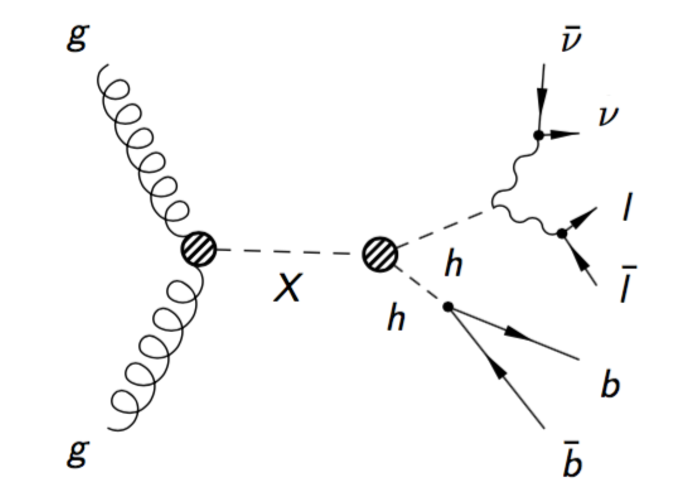
\includegraphics[width=0.45\textwidth]{figures/BGtoHH.pdf}
    \caption{ The Feynman diagram of the graviton production with the subsequent decay to a pair of the Higgs bosons. What follows is a decay to a pair of b quarks and Z bosons. Shown is 2 b quarks, 2 leptons, and 2 neutrinos final state.
    }
    \label{fig:BGtoHH}
  \end{center}
\end{figure}


\subsection{Analysis Strategy}

The analysis is based on ntuples and object selection from the approved VHbb sister analysis~\cite{VHbb_inspire}. Leptons, b jets, and the missing transverse energy (MET) are reconstructed using the standard CMS procedures~\cite{CMSreco} and the Particle Flow (PF) algorithm~\cite{PFalgo}. b-jets are identified using the Combined MVA v2 (CMVA) algorithm~\cite{BTagtwiki}. Then, on shell Z bosons are selected of dilepton pairs with a net charge zero for a pair. Higgs boson decaying to b quarks (Hbb) is reconstructed as a pair of b jets with the highest CMVA output value. Finally, double Higgs boson transverse mass, which is used in the shape analysis to extract limits, is constructed computing the transverse mass of the sum of the Lorentz vectors of the two leptons forming the on-shell Z, MET, and a pair of the b jets forming the \HBB. An additional cut on the missing transverse energy preserves the orthogonality with the existing HIG-18-013 ``2b 2l 2q'' analysis. Lastly, the cut on the BDT is used to reduce the background contamination in the signal region.

Main backgrounds are \ttbar and Drell-Yan in association with jets. Their normalization is extracted during the simultaneous fit of signal region (SR), as well as control region \ttbar (CRTT), and control region Drell-Yan (CRDY). Others, minor backgrounds, are single top production, diboson samples (WW, WZ, ZZ), and ZH production. 
%We assign systematics uncertainties on the QCD scale corresponding to each process. Also uncertainty associated with the imperfect knowledge of the single top cross section is added.
 \clearpage

\section{Data and Triggers}\label{sec:data}

\subsection{Data}
This measurement uses the full dataset of 2016 collected with the CMS detector in pp collisions
at 13 TeV center-of-mass energy with the corresponding integrated lumonocity of 35.9 ~\fbinv. 

As the measurement is based on dilepton signatures, the DoubleMuon and DoubleElectron primary
datasets are analyzed and only on-shell \Zll decays are considered, where $\ell=\Pe, \Pgm$.
 
The run periods and the corresponding integrated luminosities are listed in Table ~\ref{tab:datasets} for DoubleMuon channel, DoubleElectron channel is similar.
\begin{table}[htbp]
\caption{List of used 2016 DoubleMuon data sets.
%\lumi16  across all modes.  
An uncertainty of $2.5\%$ is  assigned for the 2016 data set luminosity~\cite{lumiUnc}}

\label{tab:datasets}
\begin{center}
\scalebox{0.9}{
\begin{tabular}{|c|c|} \hline%\hline
Dataset       & $\int\cal L$ (\fbinv) \\
\hline
%{\tt DoubleMuon\_Run2016B-03Feb2017-v1}       & \multirow{2}{*}{$\sim$5.9}  \\
{\tt DoubleMuon\_Run2016B-03Feb2017-v2}       & {$\sim$5.9}  \\
%{\tt DoubleMuon\_Run2016B-03Feb2017-v2}       &   \\
{\tt DoubleMuon\_Run2016C-03Feb2017-v1}       & $\sim$2.7 \\
{\tt DoubleMuon\_Run2016D-03Feb2017-v1}       & $\sim$4.3 \\
{\tt DoubleMuon\_Run2016E-03Feb2017-v1}       & $\sim$4.1 \\
{\tt DoubleMuon\_Run2016F-03Feb2017-v1}       & $\sim$3.2 \\
{\tt DoubleMuon\_Run2016G-03Feb2017-v1}       & $\sim$3.8 \\
{\tt DoubleMuon\_Run2016H-03Feb2017-v1}       & $\sim$11.8 \\
\hline
Total Lumi                        & 35.9 \\
\hline%\hline
\end{tabular}
}
\end{center}
\end{table}

\subsection{Triggers\label{sec:triggers}}
%% Because the analysis is performed in the dielectron and dimuon channels, unprescaled dilepton 
%% triggers with the lowest available transverse momentum thresholds are utilized. The triggers at the L1 and
%% HLT level are listed in table ~\\ref{tab:trgs2015}. Dielectron trigger requires the leading electron to pass $23$ GeV $p_{T}$ cut and $12$ GeV $p_{T}$ cut for the subleading electron. Offline cuts are $25$ GeV $p_{T}$ cut and $15$ GeV $p_{T}$ cut correspondinly. Dimuon triggers require the leading muon to pass $17$ GeV $p_{T}$ cut and $8$ GeV $p_{T}$ cut for the subleading muon with the $20$ GeV $p_{T}$ cut and $15$ GeV $p_{T}$ cut for offline selection correspondinly. $\eta$ region in the gap is excluded (1.4442 to 1.566). 

Because the analysis is performed in the dielectron and dimuon channels, unprescaled dilepton
triggers with the lowest available transverse momentum thresholds are utilized. The triggers at the L1 and
HLT level are listed in Table ~\ref{tab:trgs2015}. Dielectron trigger requires the leading electron to pass $23$ GeV $p_{T}$ cut and $12$ GeV $p_{T}$ cut for the subleading electron, both electrons should be within $\eta < $ 2.5. Dimuon triggers require the leading muon to pass $17$ GeV $p_{T}$ cut and $8$ GeV $p_{T}$ cut for the subleading muon, both muons should be within $\eta < $  2.4. $\eta$ region in the gap is excluded (1.4442 to 1.566).



\begin{table}[b]
\caption{Triggers for dimuon and dielectron analysis channels both at L1 and HLT levels.}
% In parenthesis we report the threshold used for data after run2016D.                                                                                                                                    

\label{tab:trgs2015}
\begin{center}
\scalebox{0.75}{
\begin{tabular}{|c|c|c|} \hline%\hline

 Channel                    & L1 Seeds                 & HLT Paths                                                         \\ \hline
 Z$(\Pgm\Pgm)$~\Znn \HBB       & {\tt L1\_SingleMu20}          & {\tt HLT\_Mu17\_TrkIsoVVL\_Mu8\_TrkIsoVVL\_v* OR}                    \\
                              & {\tt }                        & {\tt HLT\_Mu17\_TrkIsoVVL\_TkMu8\_TrkIsoVVL\_v* OR}         \\
                              & {\tt }                        & {\tt HLT\_Mu17\_TrkIsoVVL\_Mu8\_TrkIsoVVL\_DZ\_v* OR}         \\
                              & {\tt }                        & {\tt HLT\_Mu17\_TrkIsoVVL\_TkMu8\_TrkIsoVVL\_DZ\_v*}         \\ \hline

 Z$(\Pe\Pe)$~\Znn \HBB         & {\tt L1\_SingleEG30      OR}  & {\tt HLT\_Ele23\_Ele12\_CaloIdL\_TrackIdL\_IsoVL\_DZ } \\
                              & {\tt L1\_SingleIsoEG22er OR}  & {\tt  }         \\
                              & {\tt L1\_SingleIsoEG24   OR}  & {\tt  }         \\
                              & {\tt L1\_DoubleEG\_15\_10  }  & {\tt  }         \\ \hline
%\hline%\hline
\end{tabular}
}

\end{center}
\end{table}

Before measuring trigger scale factors, ID and ISO cuts are applied, as well as $p_{T}$ cuts of the offline selection. For dielectron trigger leading and subleading electrons have to pass $25$ GeV $p_{T}$ cut and $15$ GeV $p_{T}$ cut correspondinly. Dimuon triggers require the leading muon to pass $20$ GeV $p_{T}$ cut and $15$ GeV $p_{T}$ cut for the subleading muon. 
Dilepton scale factor have been computed for each leg separately, since the cuts on each leg vary (Fig. ~\ref{fig:trigger_eff_diele}). Following the recommendations from the Muon POG, scale factors have been computed separately for two groups: run H and other runs, and then the luminosity averaged scale factors are calculated (Figs. ~\ref{fig:trigger_SF_dimu_BCDEFG}, ~\ref{fig:trigger_SF_dimu_H}, ~\ref{fig:trigger_SF_dimu_dZ_H}). 

\begin{figure}
\centering
\subfloat[][Leg 1]
{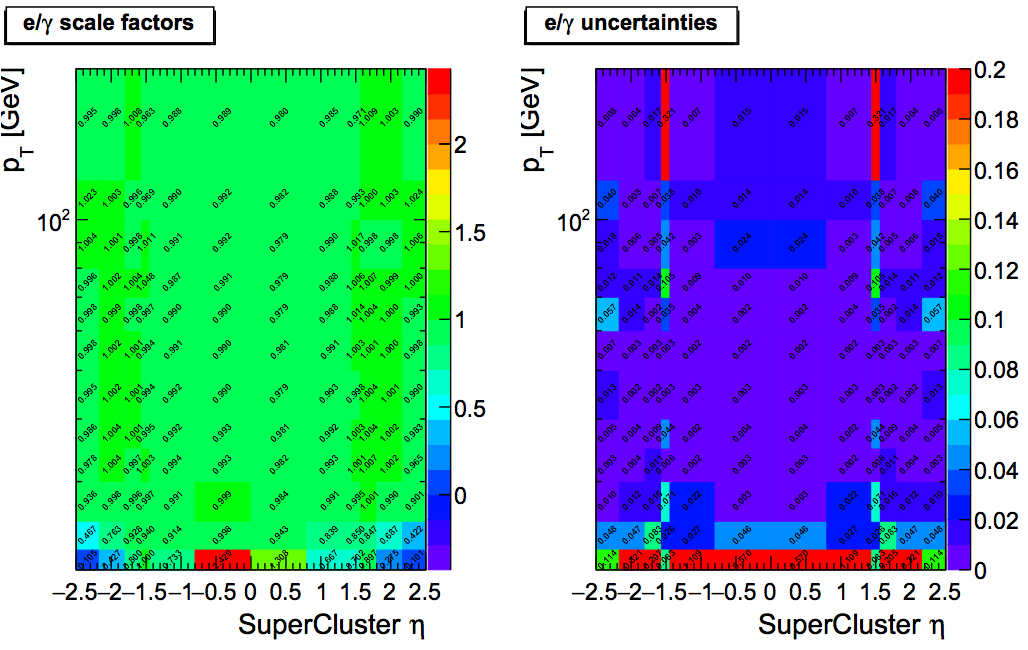
\includegraphics[width=1.0\textwidth]{figures/trigger/electronTriggerEfficiencyelectronTriggerEfficiencyHLT_Leg1_WP90_2016.png} } \\
\subfloat[][Leg 2]
{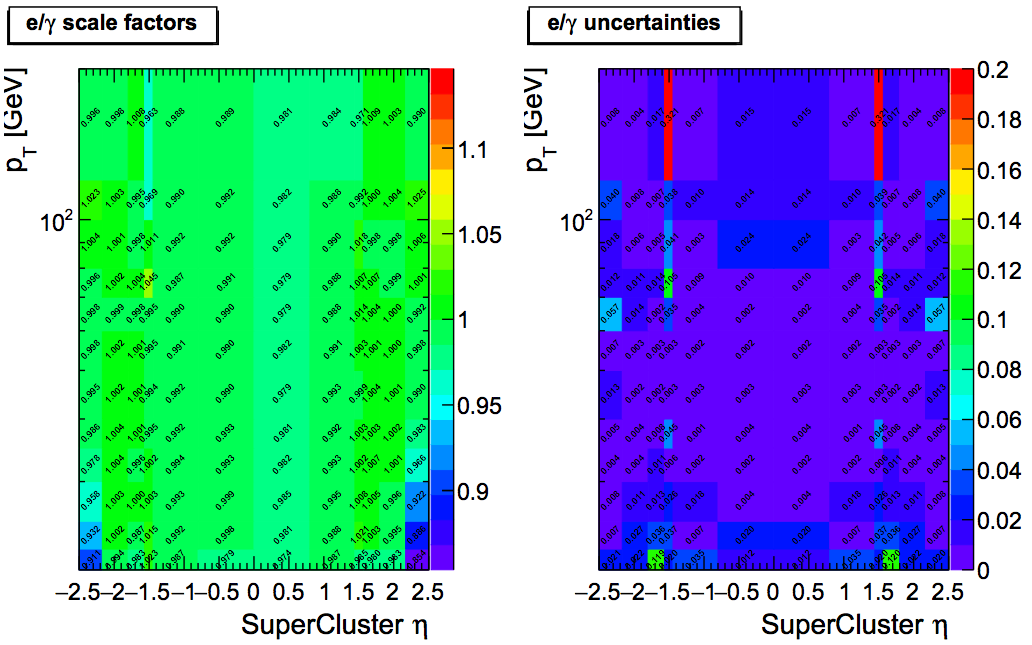
\includegraphics[width=1.0\textwidth]{figures/trigger/electronTriggerEfficiencyelectronTriggerEfficiencyHLT_Leg2_WP90_2016.png} } \\
\caption{Electron scale factors in $p_{T}$ and $\eta$ bins for 2016 data set for the HLT\_Ele23\_Ele12\_CaloIdL\_TrackIdL\_IsoVL\_DZ trigger. ID cut (general purpose MVA WP90) and ISO cuts are applied, then the scale factors are measured. Taken from ~\cite{vhbbAN}}
\label{fig:trigger_eff_diele}
\end{figure}


\begin{figure}
\centering
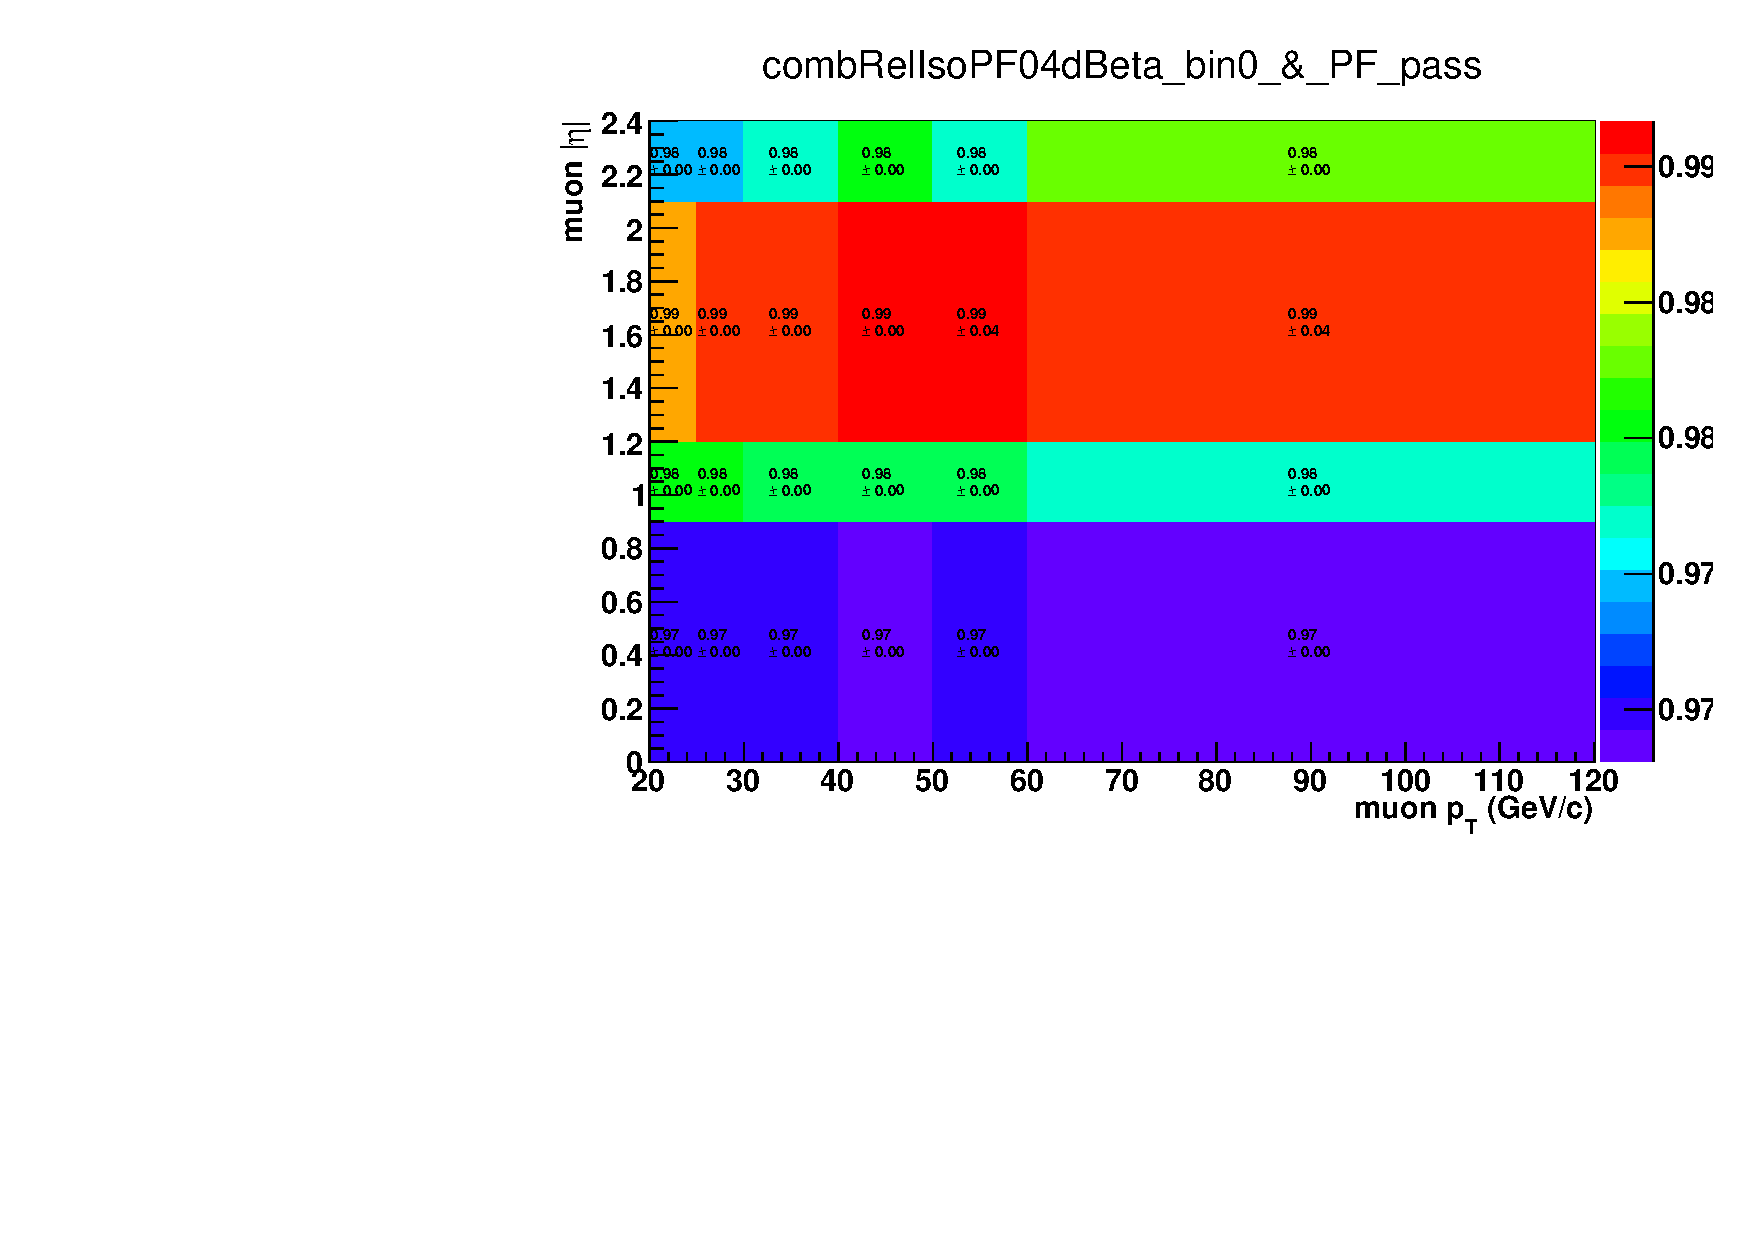
\includegraphics[width=0.475\textwidth]{figures/trigger/Run_BCDEFG_PlotSF_hlt_Mu17_Mu8_OR_TkMu8_leg8_NUM_hlt_Mu17_Mu8_OR_TkMu8_leg8_DEN_LooseIDnISO_PAR_pt_eta_pt_abseta_ratio.pdf}
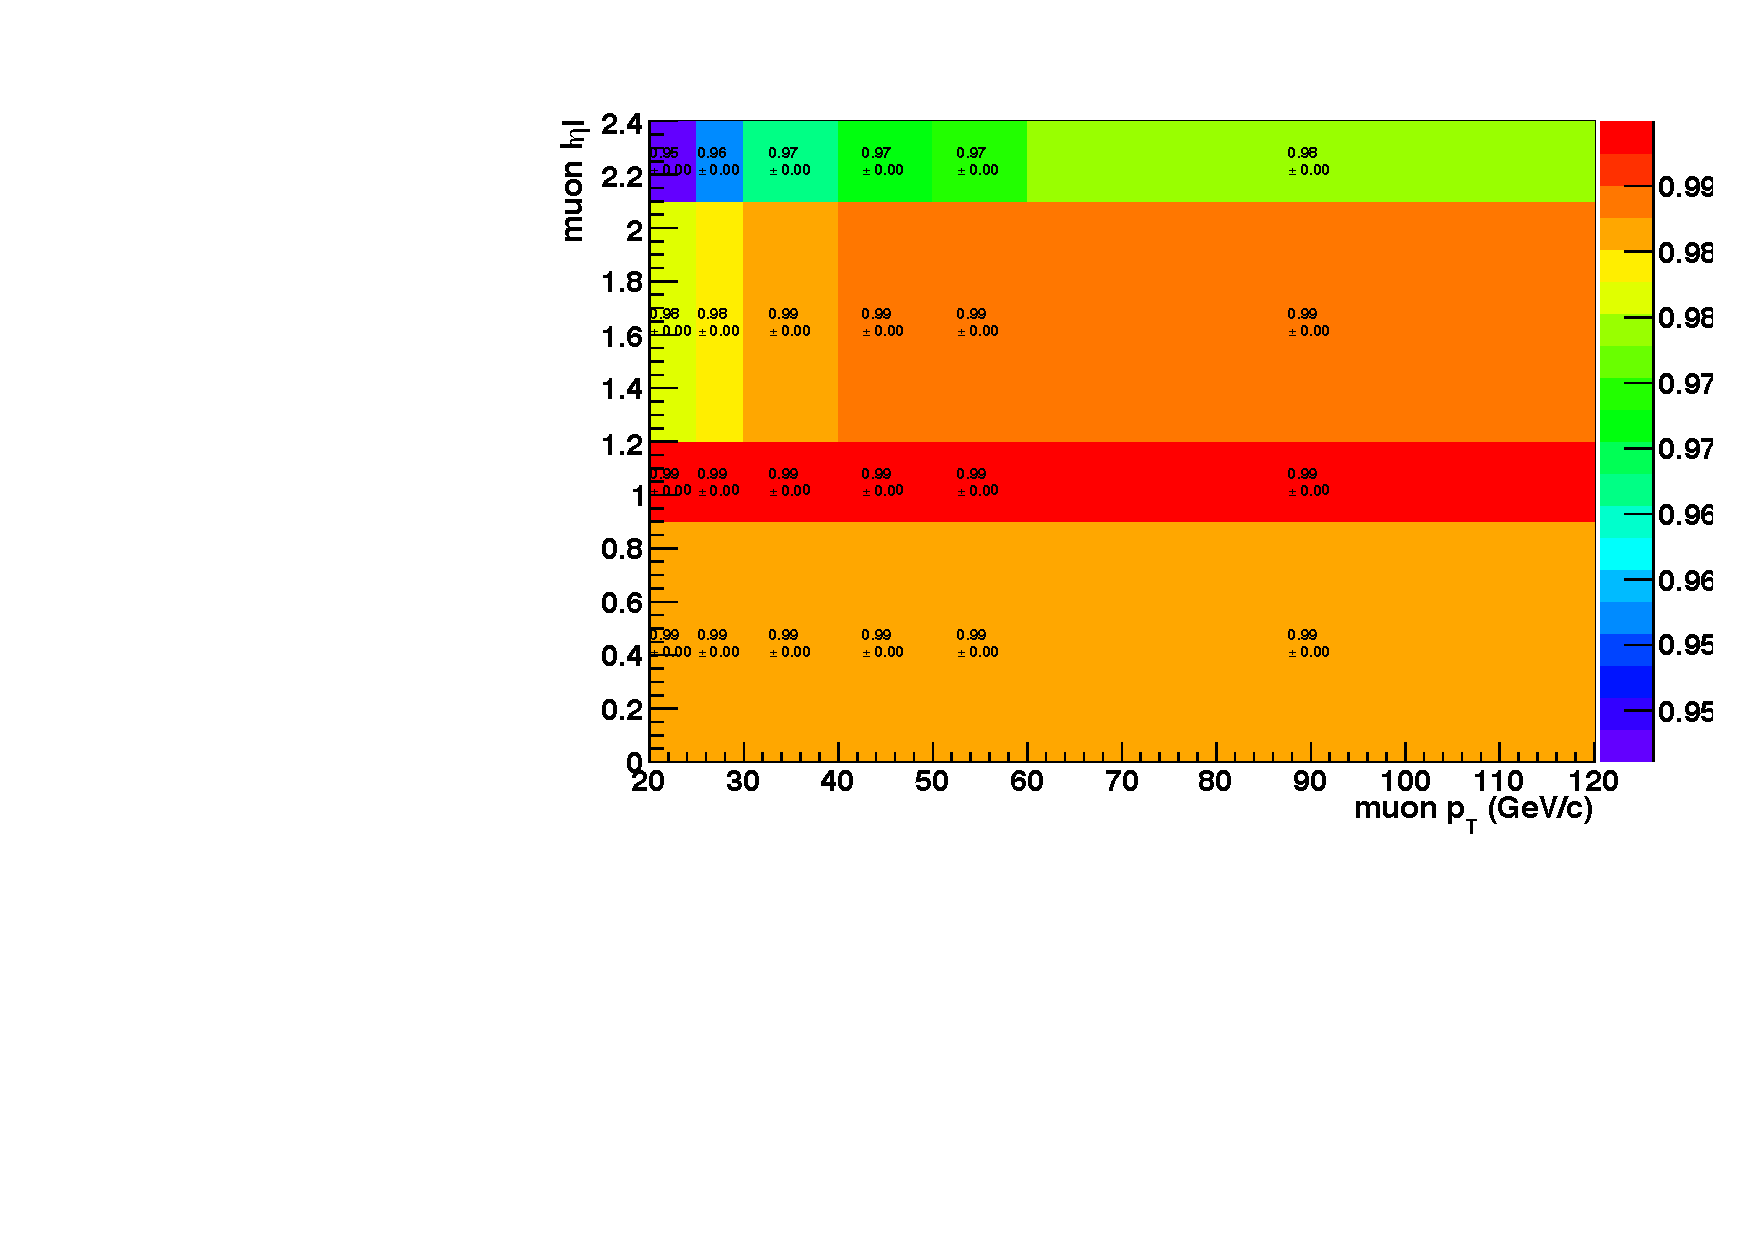
\includegraphics[width=0.475\textwidth]{figures/trigger/Run_BCDEFG_PlotSF_hlt_Mu17Mu8_leg17_NUM_hlt_Mu17Mu8_leg17_DEN_LooseIDnISO_PAR_pt_eta_pt_abseta_ratio.pdf}\\
\caption{Muon scale factors in $p_{T}$ and $\eta$ bins for 2016 data runs B, C, D, E, F, G for the  HLT\_Mu17\_TrkIsoVVL\_Mu8\_TrkIsoVVL\_v* OR HLT\_Mu17\_TrkIsoVVL\_TkMu8\_TrkIs\
oVVL\_v* triggers. Left: Scale factors for 8 GeV leg. Right: Scale factors for 17 GeV leg, provided that the subleading leg passed 8 GeV cut.}
\label{fig:trigger_SF_dimu_BCDEFG}
\end{figure}

\begin{figure}
\centering
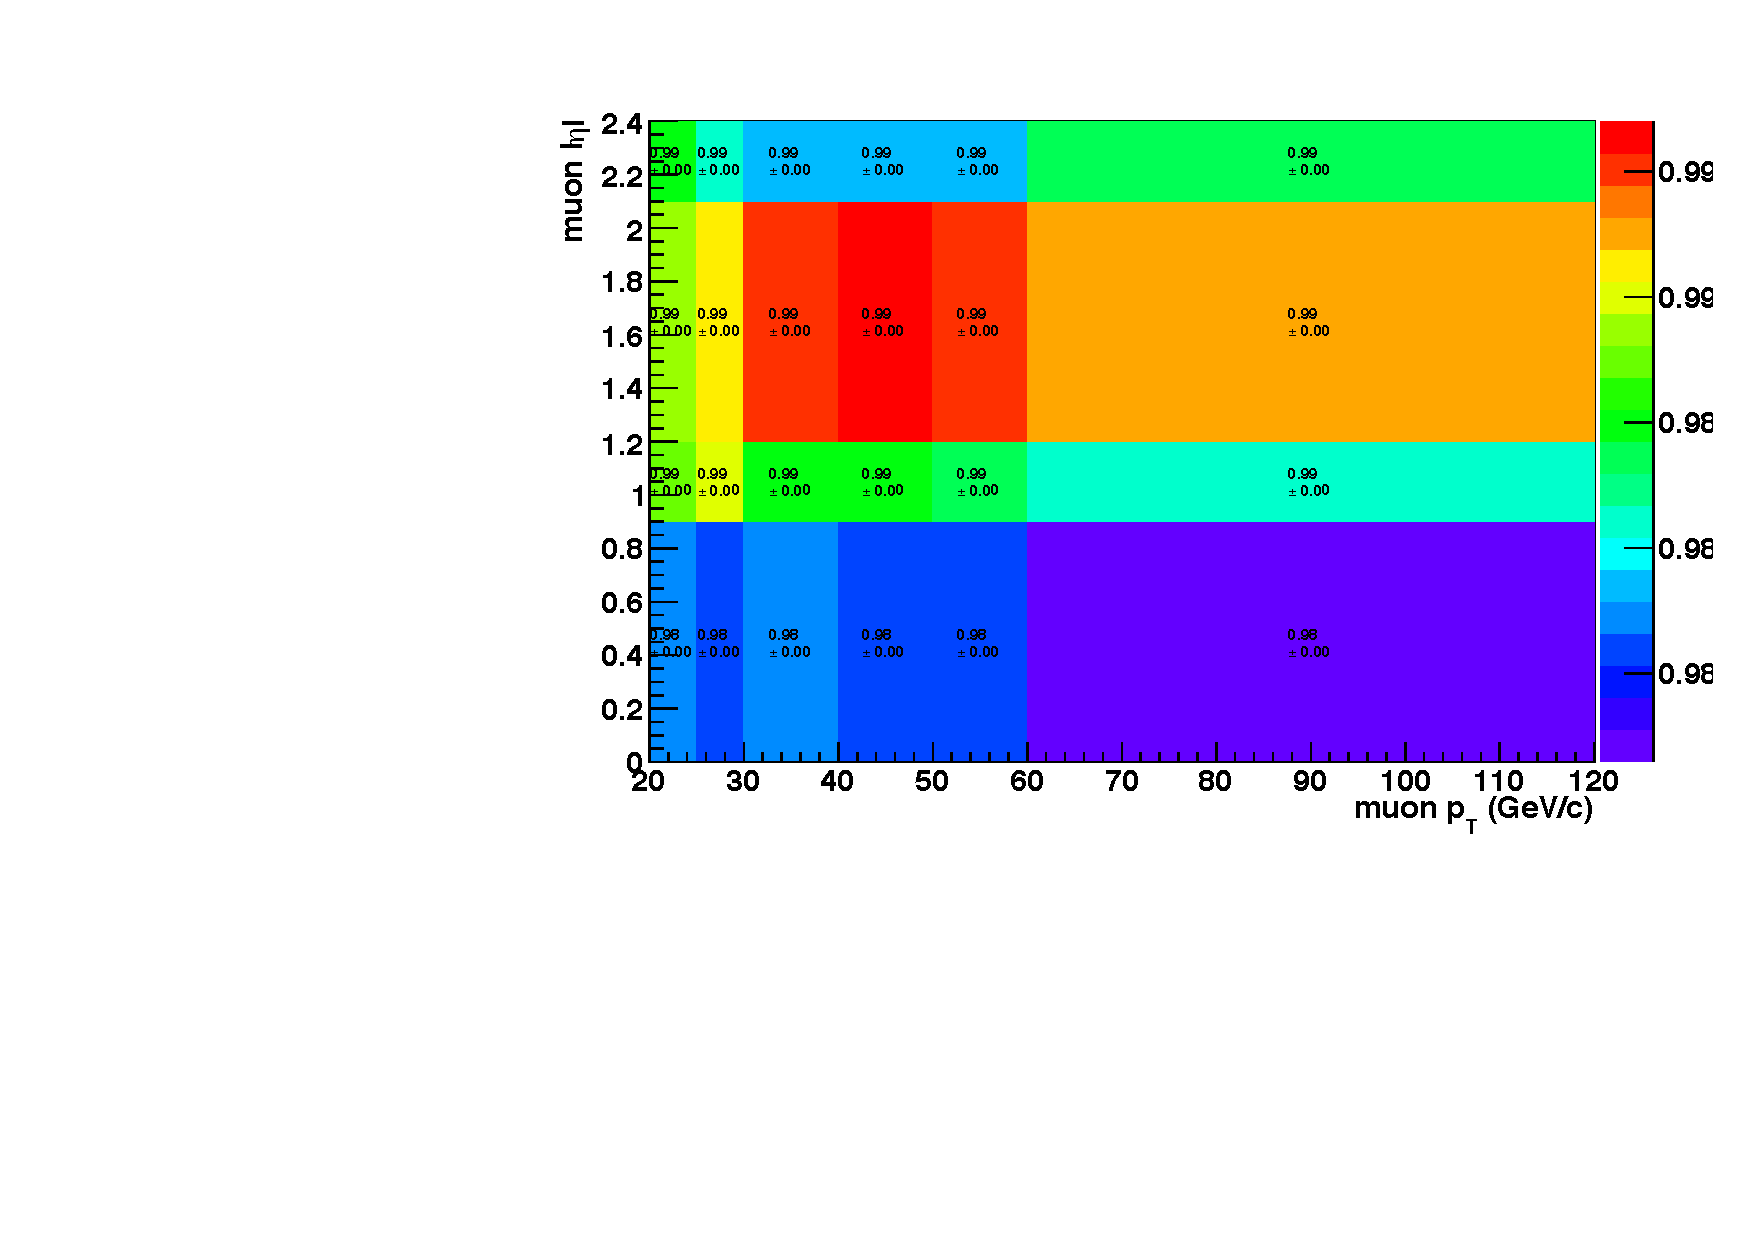
\includegraphics[width=0.475\textwidth]{figures/trigger/Run_H_PlotSF_hlt_Mu17_Mu8_OR_TkMu8_leg8_NUM_hlt_Mu17_Mu8_OR_TkMu8_leg8_DEN_LooseIDnISO_PAR_pt_eta_pt_abseta_ratio.pdf}
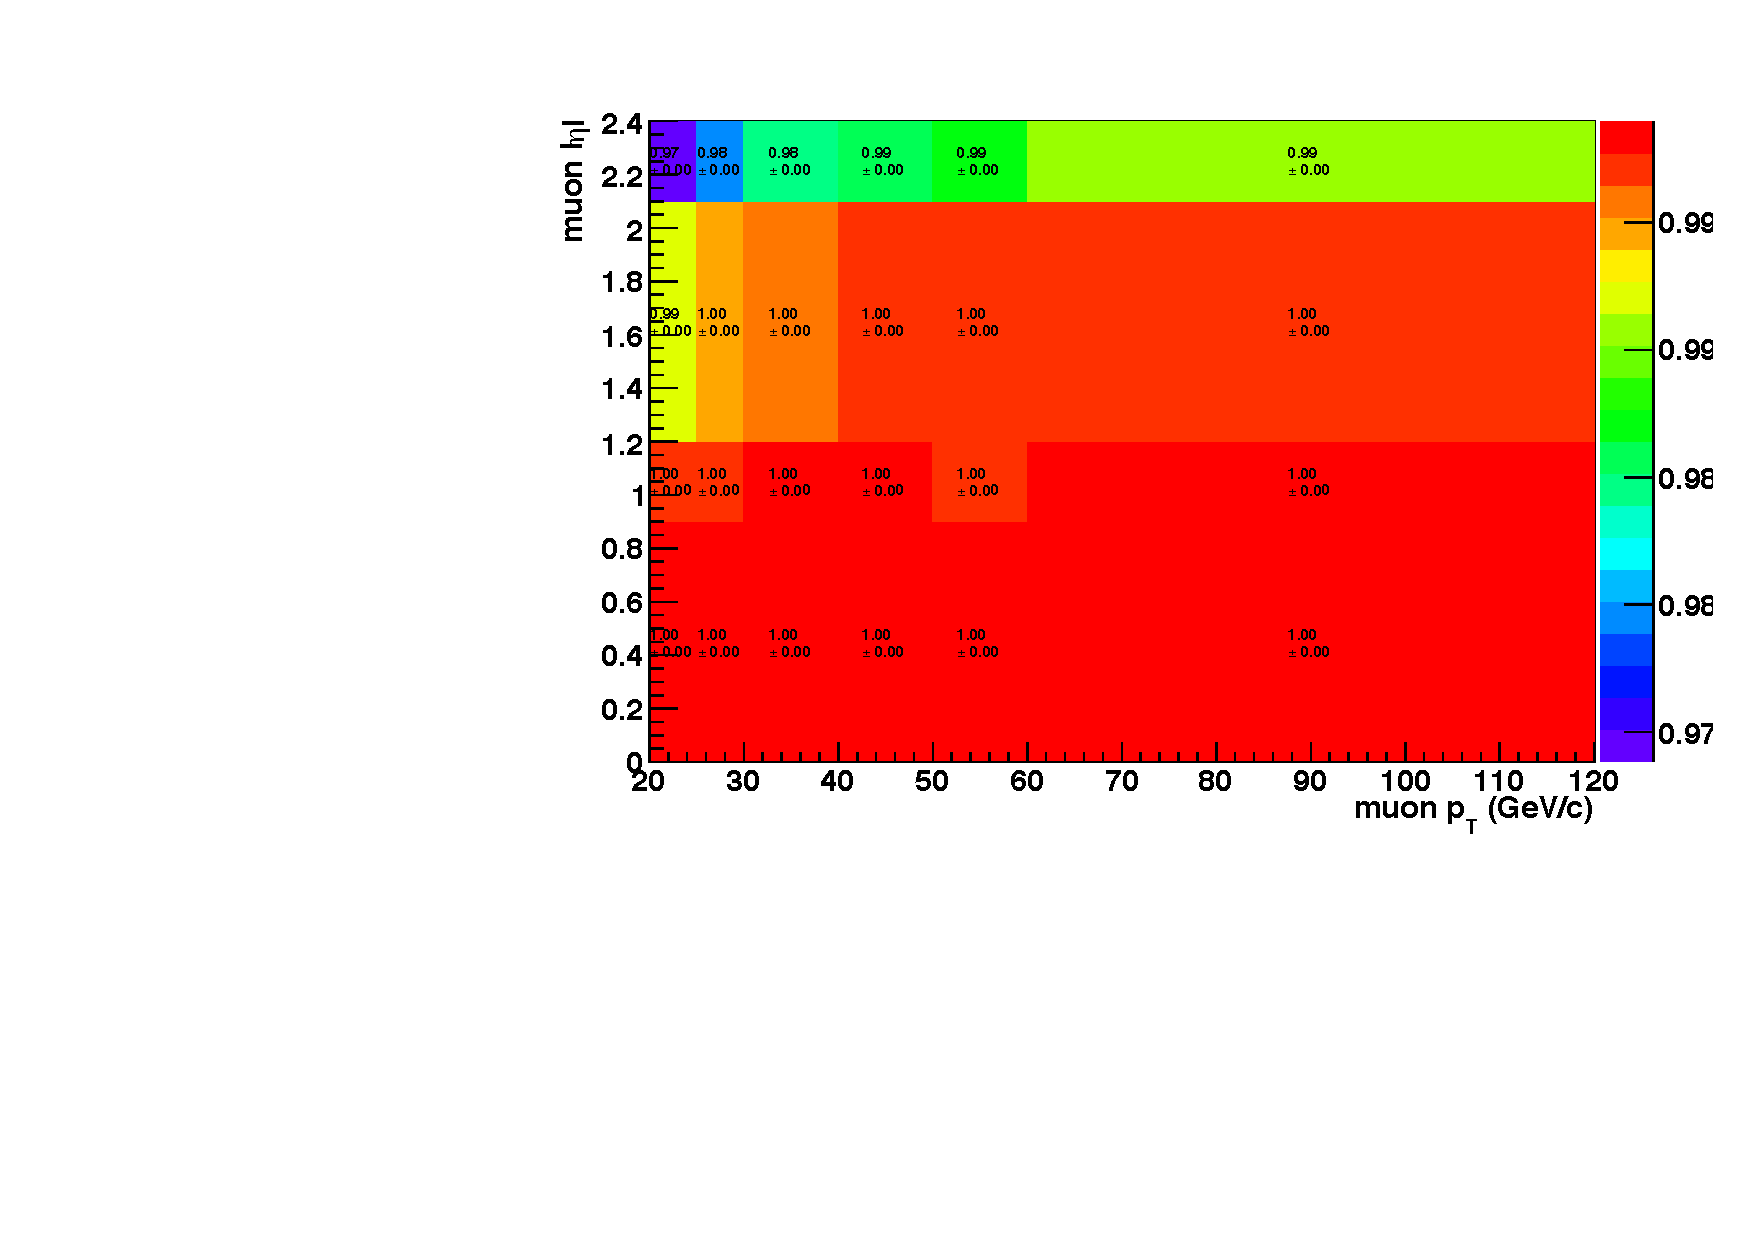
\includegraphics[width=0.475\textwidth]{figures/trigger/Run_H_PlotSF_hlt_Mu17Mu8_leg17_NUM_hlt_Mu17Mu8_leg17_DEN_LooseIDnISO_PAR_pt_eta_pt_abseta_ratio.pdf}\\
\caption{Muon scale factors in $p_{T}$ and $\eta$ bins for 2016 data run H for the  HLT\_Mu17\_TrkIsoVVL\_Mu8\_TrkIsoVVL\_v* OR HLT\_Mu17\_TrkIsoVVL\_TkMu8\_TrkIs\
oVVL\_v* triggers. Left: Scale factors for 8 GeV leg. Right: Scale factors for 17 GeV leg, provided that the subleading leg passed 8 GeV cut.}

\label{fig:trigger_SF_dimu_H}
\end{figure}

\begin{figure}
\centering
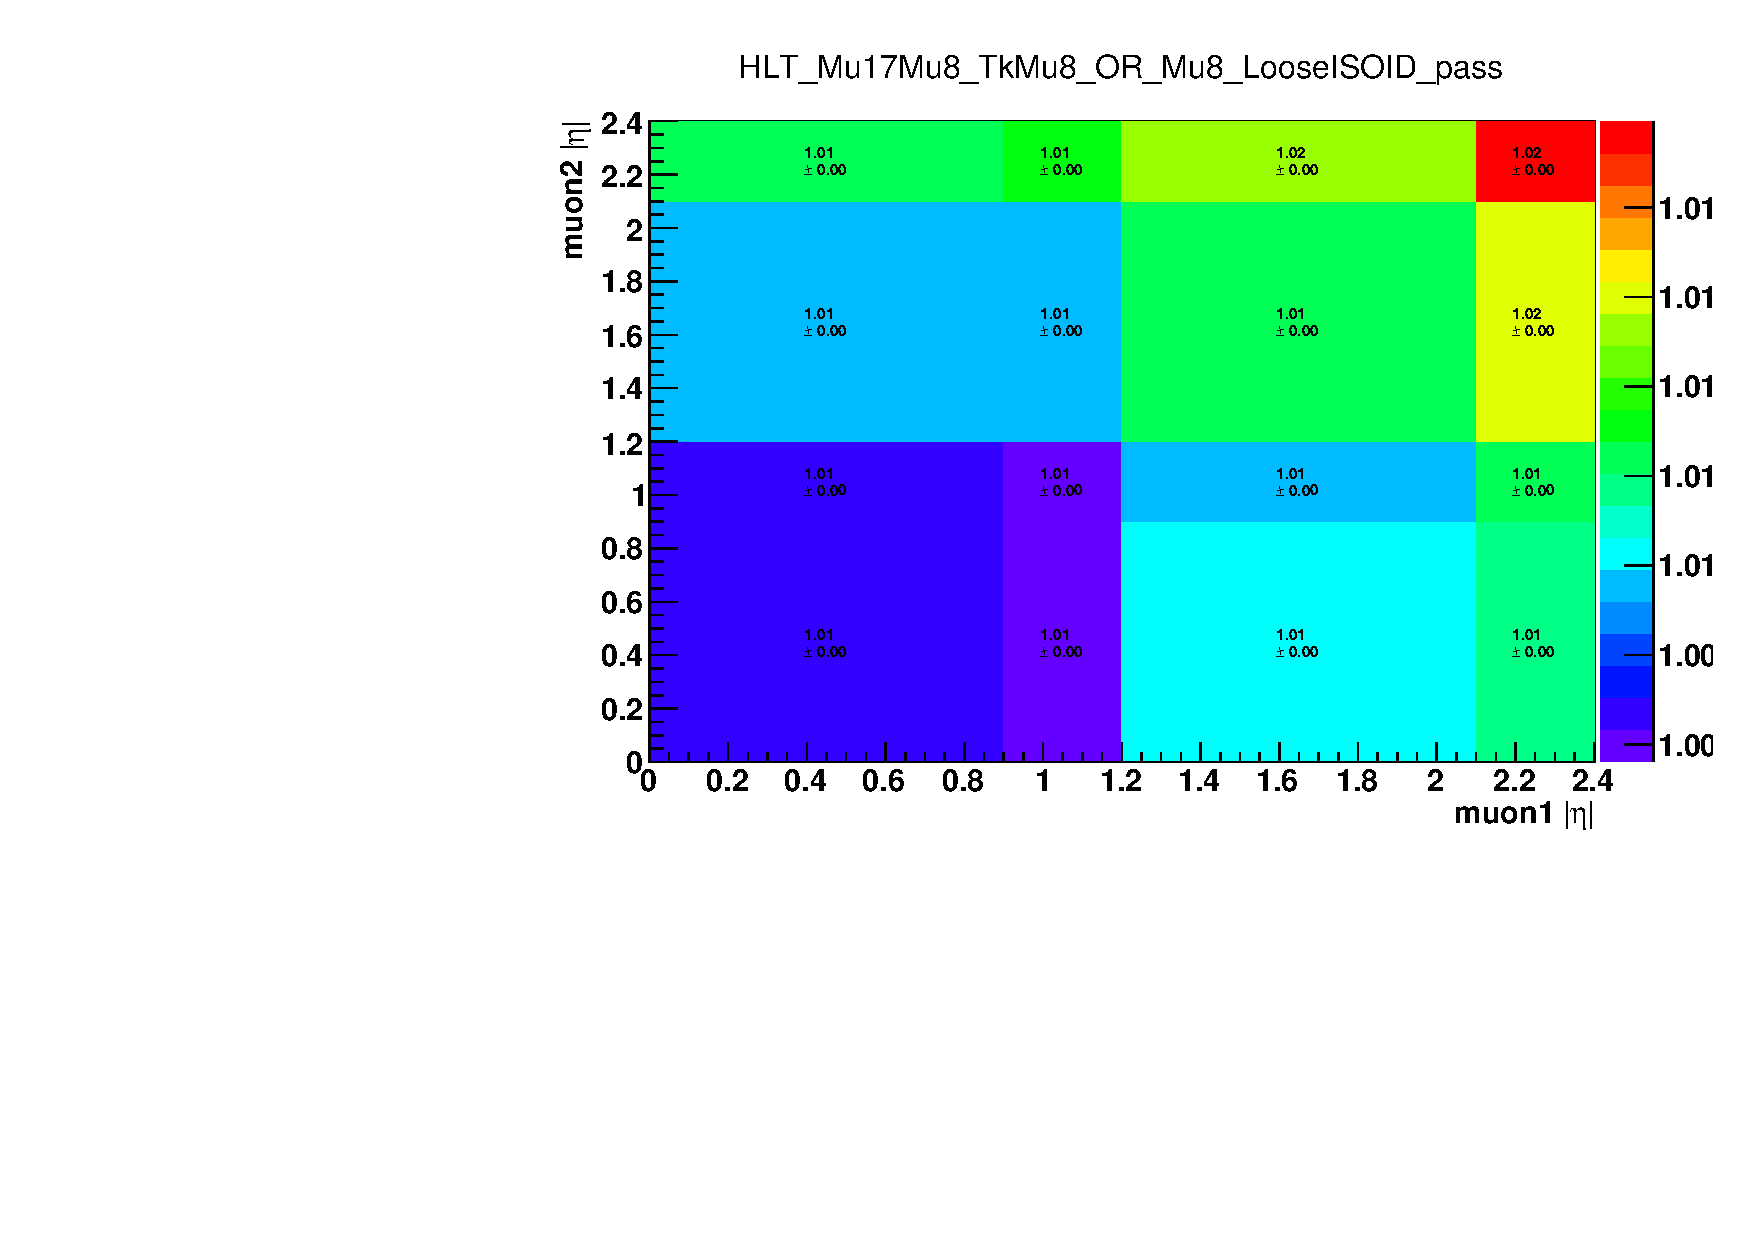
\includegraphics[width=0.85\textwidth]{figures/trigger/PlotSF_dZ_NUM_dZ_DEN_hlt_Mu17_Mu8_OR_TkMu8_loose_PAR_eta1_eta2_abseta_tag_abseta_ratio.pdf}
\caption{Scale factors in $\eta$ bins of the leading and subleading muons for 2016 data set for dZ requirement, measured after muons have passed the HLT\_Mu17\_TrkIsoVVL\_Mu8\_TrkIsoVVL\_v* OR HLT\_Mu17\_TrkIsoVVL\_TkMu8\_TrkIsoVVL\_v* triggers. }
\label{fig:trigger_SF_dimu_dZ_H}
\end{figure}



\begin{figure}
\centering
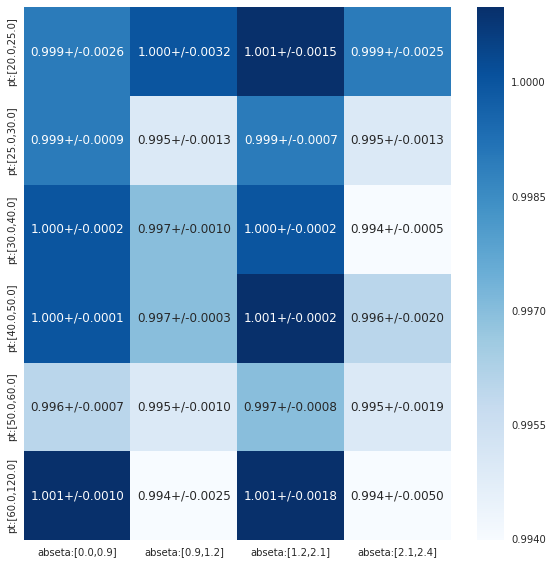
\includegraphics[width=0.5\textwidth]{figures/muon_ID_BCDEFv2.png}
\bigbreak
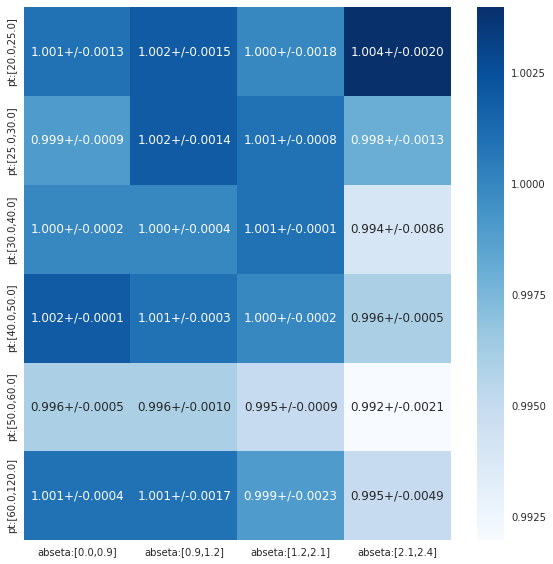
\includegraphics[width=0.5\textwidth]{figures/muon_ID_GHv2.png}
\caption{ Muon ID scale factors in $p_{T}$ and $\eta$ bins. Left: runs B to F. Right: runs G and H.}
\label{fig:muonID_SF}
\end{figure}

\newline
\newline

\begin{figure}
\centering
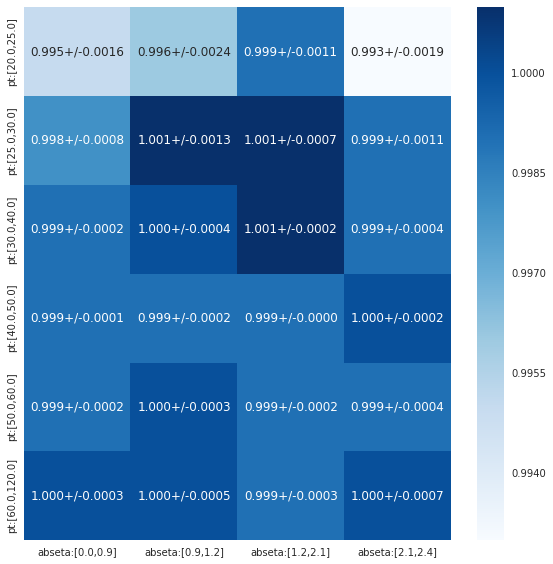
\includegraphics[width=0.5\textwidth]{figures/muon_ISO_BCDEFv2.png}
\bigbreak
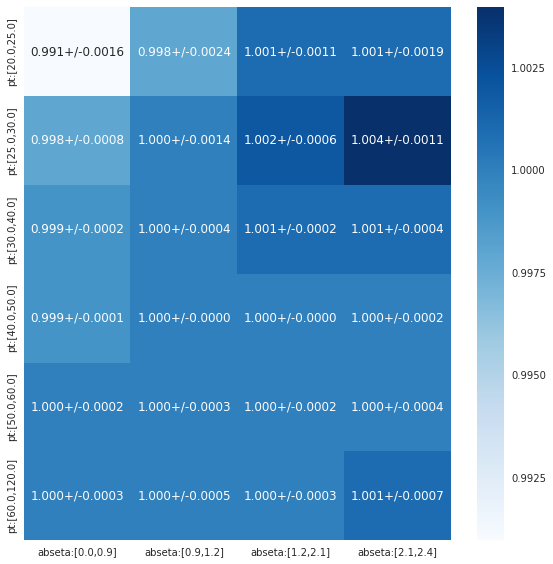
\includegraphics[width=0.5\textwidth]{figures/muon_ISO_GHv2.png}
\caption{ Muon ISO scale factors in $p_{T}$ and $\eta$ bins. Left: runs B to F. Right: runs G and H.}
\label{fig:muonISO_SF}
\end{figure}

\newline
\newline

\begin{figure}
\centering
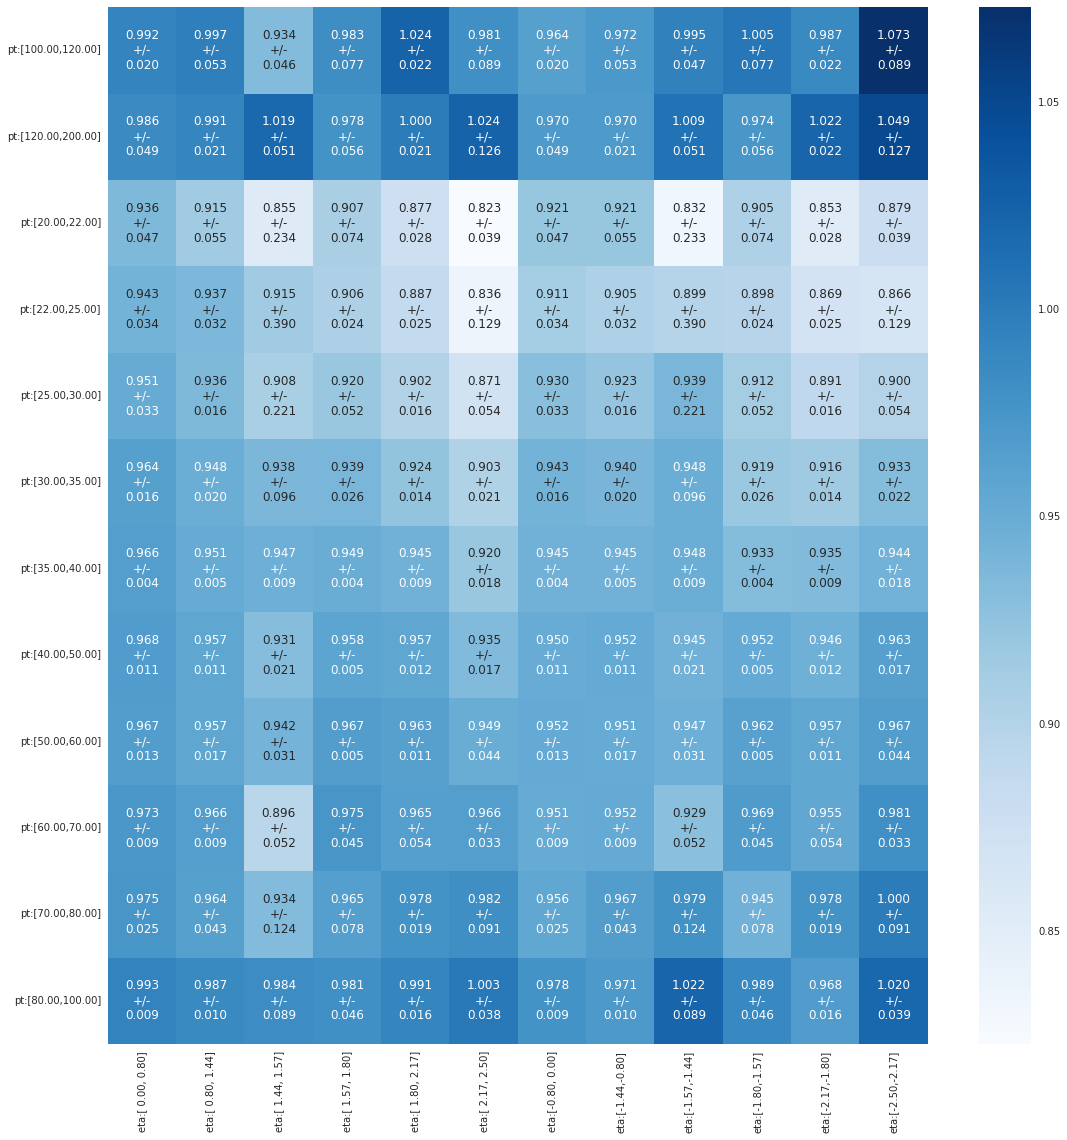
\includegraphics[width=0.9\textwidth]{figures/EIDISO_ZH_out.png}
\caption{ Electron ID+ISO scale factors in $p_{T}$ and $\eta$ bins.}
\label{fig:muonID_SF}
\end{figure}

 \clearpage

\section{Simulated Samples}\label{sec:samples}

%\subsection{Monte~Carlo samples\label{sec:mc}}

\subsection{Signal simulation\label{sec:signalMC}}

MC signal samples of the resonant Higgs boson pair production have been generated at the Leading Order (LO) using the \MADGRAPH~5 version\ ~2.2.2.0  generator ~\cite{Alwall:2014hca}. The gluon fusion production of a heavy narrow resonance is followed by the decay of the resonance into two SM Higgs bosons whose mass is fixed at 125~GeV.

Two signal MC samples are generated to cover the Higgs decay modes contributing to the 2 b jets 2 leptons 2 neutrinos final state of this measurement. The first sample type is a HH decay in to bbZZ channel, where one Higgs boson decays to a pair of b-quarks and the second Higgs boson decays into two Z bosons. In the second sample type bbVV events are generated, where HH can decay through bbWW and bbZZ channels. For both samples, the Z boson-pair and the W boson-pair are set to decay leptonically to two leptons and two neutrinos, where a lepton could be an electron or a muon. The second, bbVV, sample is filtered using the generator level information such that only the events with a W-boson pair (bbWW) are kept, while the Z-pair events are dropped: there are very few of them in the bbVV sample, and most importantly, high statistics bbZZ is taken from the dedicated bbZZ sample of the first type.

Events in the signal bbZZ and bbWW MC samples are normalised to 2~pb HH production cross section, which is a typical value of the heavy resonance production at 300 GeV predicted by the WED. Additionally the normalization includes the branching ratios of the Higgs boson decays contributing to the final state studied here: 0.0012 and 0.0266 for $HH\to bbZZ\to bb\ell\ell\nu\nu$ and $HH\to bbWW\to bb\ell\nu\ell\nu$, respectively \cite{CERNYR4}.

%%There are ten samples in the mass range of 260 to 1000 GeV generated for bbVV analysis and 16 samples for bbZZ from 250 GeV to 1000 GeV. Therefore, this document presents results for the masses where both signals are present. In the future we would consider doing approximations of the bbWW contribution where we have missing samples or generate them privately.

Unless mentioned otherwise, throughout the text plots and numbers represent the graviton study. The data and backgrounds for the radion measurement are the same, thus distributions also show the same good Data MC agreement and can be found for at Figs. ~\ref{fig:MCcomparisons} for the graviton case and ~\ref{fig:MCcomparisons_radion} for the radion case.

\subsection{Background simulation\label{sec:bkgMC}}

In this analysis the main backgrounds are \ttbar and Drell-Yan plus
jets with the mass of the boson greater than 50 GeV. Not all the
background processes pass our tight preselection (see section ~\ref{hhSelection}),
those which do, are single top, dibosons, and ZH backgrounds that are
listed in the Table \ref{tab:bg_mcsamples}:

\begin{table}[htbp]%H]
  %\footnotesize
  \begin{center}
    \caption{Background Monte Carlo samples\label{tab:bg_mcsamples}}
    \begin{tabular}{|c|}%|l|r|r|r|r|r|}
      \hline
      % Sample  & Generator & $m_{H} (\GeV/c^2)$ & $\sigma$ (pb) & events &  $\int\cal L$ (\fbinv) \\
      %\hline
      \multicolumn{5}{|l|}{\texttt{DY1JetsToLL\_M-50\_TuneCUETP8M1\_13TeV-madgraphMLM-pythia8}} \\
%                & \MADGRAPH\,5+\PYTHIA{}\,8 & 725 & 39 800 000 & 54.5 \\
      \multicolumn{5}{|l|}{\texttt{DY2JetsToLL\_M-50\_TuneCUETP8M1\_13TeV-madgraphMLM-pythia8}} \\
%               & \MADGRAPH\,5+\PYTHIA{}\,8 & 725 & 39 800 000 & 54.5 \\
      %\hline
      \multicolumn{5}{|l|}{\texttt{DY3JetsToLL\_M-50\_TuneCUETP8M1\_13TeV-madgraphMLM-pythia8}} \\
%              & \MADGRAPH\,5+\PYTHIA{}\,8 & 394.5 & 19 400 000  & 50.2 \\
      %\hline
      \multicolumn{5}{|l|}{\texttt{DY4JetsToLL\_M-50\_TuneCUETP8M1\_13TeV-madgraphMLM-pythia8}} \\
%             & \MADGRAPH\,5+\PYTHIA{}\,8 & 96.47 & 4 960 000 & 52.2 \\
      \multicolumn{5}{|l|}{\texttt{WW\_TuneCUETP8M1\_13TeV-pythia8}} \\
%            & \PYTHIA{}\,8 & 118.7 & 993 640 &  8.37  \\
      %\hline
      \multicolumn{5}{|l|}{\texttt{WZ\_TuneCUETP8M1\_13TeV-pythia8}} \\
%           & \PYTHIA{}\,8 & 47.13    &   1 000 000   &   21.22  \\
      %\hline
      \multicolumn{5}{|l|}{\texttt{ZZ\_TuneCUETP8M1\_13TeV-pythia8}} \\
%          & \PYTHIA{}\,8 & 16.523     &   985 600   &   59.65  \\
       \multicolumn{5}{|l|}{\texttt{ZH\_HToBB\_ZToLL\_M125\_13TeV\_aMC@NLO}} \\
      %\hline
      \multicolumn{5}{|l|}{\texttt{TT\_TuneCUETP8M1\_13TeV-powheg-pythia8}} \\
       %         & \POWHEG+\PYTHIA{}\,8 & 831.76   & 187 626 200 + 97 994 442&  343  \\
      %\hline
      \multicolumn{5}{|l|}{\texttt{ST\_tW\_top\_5f\_inclusiveDecays\_13TeV-powheg-pythia8\_TuneCUETP8M1}} \\
        %        & \POWHEG+\PYTHIA{}\,8 & 35.6   &   1 000 000   &   28.09  \\
      %\hline
      \multicolumn{5}{|l|}{\texttt{ST\_tW\_antitop\_5f\_inclusiveDecays\_13TeV-powheg-pythia8\_TuneCUETP8M1}} \\
         %       & \POWHEG+\PYTHIA{}\,8 & 35.6   &   999 400   &   28.07  \\
      %\hline\hline
      \multicolumn{5}{|l|}{\texttt{ST\_t-channel\_top\_4f\_leptonDecays\_13TeV-powheg-pythia8}} \\
          %      & \POWHEG+\PYTHIA{}\,8 & 136*0.325   &   999 400   &   22.6 \\
      %\hline
      \multicolumn{5}{|l|}{\texttt{ST\_t-channel\_antitop\_4f\_leptonDecays\_13TeV-powheg-pythia8}} \\
           %     & \POWHEG+\PYTHIA{}\,8 & 81*0.325   & 1 695 400 &  64.4 \\
      %\hline\hline
      \multicolumn{5}{|l|}{\texttt{ST\_s-channel\_4f\_leptonDecays\_13TeV-amcatnlo-pythia8}} \\
      %    & \POWHEG+\PYTHIA{}\,8 & 10.32   &   998 400   &   96.74  \\
\hline%\hline

    \end{tabular}
  \end{center}
  %\label{backgrounds} 
\end{table}



The simulated samples of the background processes such as 
~\ttbar~\cite{Frixione:2007nw} and the single top tW and t-channel
production processes~\cite{Frederix:2012dh} are generated at the
next-to-leading order (NLO) with POWHEG~\cite{Alioli:2009je}, while
single top s-channel production process is generated at NLO with
\MADGRAPH. \ttbar and single top production cross sections are
rescaled to the next-to-next-to-leading order (NNLO). 
Drell-Yan (DY)
process samples in association with 1, 2, 3 or 4 jets are generated
at the leading order using \MADGRAPH with the MLM
matching~\cite{Alwall:2007fs} and rescaled to NNLO using~\textsc{fewz}
program~\cite{Gavin:2010az,Li:2012wna,Gavin:2012sy}. 

As for the electroweak (EWK) order, DY samples have been rescaled to EWK NLO order with the NLO/LO k-factor of 1.23~\cite{DYkfactor}. Diboson samples
are generated at LO with {\PYTHIA}8.212~\cite{Sjostrand:2007gs}.

The main background
       process, which involves SM Higgs boson, is an associated
       production of the Higgs boson with a Z boson (ZH).  ZH process
       is simultated using the generator
%{{\sc MadGraph5_aMC@NLO}}                                                                                                                                                                               
$MadGraph5\_aMC@NLO$
~\cite{cite_aMC@NLO} with FxFx
merging~\cite{Frederix:2012ps} and
rescaled to NNLO with
{\MCFM} generator~\cite{Campbell:2010ff}.


For LO and NLO samples NNPDF3.0 parton distribution functions (PDF)
set is used. {\POWHEG} and {\MADGRAPH} interfaced with
{\PYTHIA}8.212~\cite{Sjostrand:2007gs} are used for the parton
showering and hadronization steps. To describe the underlying event
CUETP9M1 set derived in \cite{Khachatryan:2015pea} is
used. \GEANTfour~\cite{GEANT4} is used to model the response of the
CMS detector.

All the final cross sections denoted as NNLO are calculated at NNLO QCD accuracies and have been computed with the tool they were generated with. They found to be in agreement with the values from the LHC Higgs cross section working group ~\cite{LHCHXSWG, xsecZH, xsecTT, xsecST, xsecVV}.

During the data taking in 2016 the average number of proton-proton interactions per bunch crossing was 24 (denoted as pile up later), and in MC samples this information has been introduced overlapping these interactions with the events of interest.



 \clearpage

\section{Physics Objects Reconstruction}\label{sec:objects}
\subsection{Jets and \cPqb\ tagging}
The analysis uses anti-\kt\ (0.4) particle-flow (PF) jets, corrected for charged hadrons not coming from the primary vertex (charged hadron subtraction), and having jet energy corrections (\verb|Summer16_23Sep2016V3|) applied as a function of the jet $E_T$ and $\eta$.
Jets are only considered if they have a transverse energy above $25\GeV$.
% FIXME Something about forward jets?

In addition, they are required to be separated from any lepton candidates passing the fakeable object selections (see Tables~\ref{tab:muonIDs} and~\ref{tab:eleIDs}) by $\Delta\mathrm{R}>0.4$.

The loose and medium working points of the CSV \cPqb-tagging algorithm are used to identify \cPqb\ jets.
Data/simulation differences in the \cPqb\ tagging performance are corrected by applying per-jet weights to the simulation, dependent on the jet \pt, eta, \cPqb\ tagging discriminator, and flavor (from simulation truth)~\cite{btagRecommTWiki}.
The per-event weight is taken as the product of the per-jet weights, including those of the jets associated to the leptons.

More details can be found in the corresponding \ttH\ documentation~\cite{CMS_AN_2016-211,CMS_AN_2017-029}.

\subsection{Lepton selection}
The lepton reconstruction and selection is identical to that used in the \ttH\ multilepton analysis, as documented in Refs.~\cite{CMS_AN_2016-211,CMS_AN_2017-029}.
For details on the reconstruction algorithms, isolation, pileup mitigation, and a description of the lepton MVA discriminator and validation plots thereof, we refer to that document.

Three different selections are defined both for the electron and muon
object identification: the \emph{Loose}, \emph{Fakeable Object},
and \emph{Tight} selection.
As described in more detail later, these are used for event level vetoes, the fake rate estimation application region, and the final signal selection, respectively.
The \pt\ of fakeable objects is defined as $0.85\times\pt(\mathrm{jet})$, where the jet is the one associated to the lepton object.
This mitigates the dependence of the fake rate on the momentum of the fakeable object and thereby improves the precision of the method.

Tables~\ref{tab:muonIDs} and~\ref{tab:eleIDs} list the full criteria for the different selections of muons and electrons.

\begin{table}[h!]
\centering
\small
\topcaption{
\label{tab:muonIDs}
Requirements on each of the three muon selections. In the cases where
the cut values change between the selections, those values are listed in the table.
Otherwise, whether the cut is applied is indicated.
For the two \ptRatio\ and CSV rows, the cuts marked with a $\dagger$ are applied to leptons that fail the lepton MVA cut, while the loose cut value is applied to those that pass the lepton MVA cut.}
\begin{tabular}{cccc}
Cut & Loose & Fakeable object & Tight \\
\hline
$|\eta| < 2.4$         & \checkmark & \checkmark         & \checkmark \\
$\pt$                  & $>5\GeV$   & $>15\GeV$          & $>15\GeV$\\
$|d_{xy}| < 0.05$ (cm) & \checkmark & \checkmark         & \checkmark \\
$|d_z| < 0.1$ (cm)     & \checkmark & \checkmark         & \checkmark \\
$\text{SIP}_{3D} < 8$  & \checkmark & \checkmark         & \checkmark \\
\miniIso $< 0.4$       & \checkmark & \checkmark         & \checkmark \\
is Loose Muon          & \checkmark & \checkmark         & \checkmark \\
%\ptRatio              & --         & $>0.3\dagger$ / -- & -- \\
jet CSV                & --         & $< 0.8484$         & $ < 0.8484$ \\
%mva electron ID       & --         & $\ddagger$         & -- \\
is Medium Muon         & --         & --                 & \checkmark \\
tight-charge           & --         & --                 & \checkmark \\
lepMVA $> 0.90$        & --         & --                 & \checkmark \\
\hline
\end{tabular}
\end{table}


\begin{table}
\centering
\small
\topcaption{
\label{tab:eleIDs}
Criteria for each of the three electron selections. In cases where the cut values change between selections, those values are listed in the table. Otherwise, whether the cut is applied is indicated. In some cases, the cut values change for different $\eta$ ranges. These ranges are $0 < |\eta| < 0.8$, $0.8 < |\eta| < 1.479$, and $1.479 < |\eta| < 2.5$ and the respective cut values are given in the form (value$_1$, value$_2$, value$_3$).
}
\resizebox{1.0\linewidth}{!}{
\begin{tabular}{cccc}
Cut & Loose & Fakeable Object & Tight \\
\hline
$|\eta| < 2.5$                                  & \checkmark & \checkmark                   & \checkmark \\
$\pt$                                           & $>7\GeV$   & $>15\GeV$                    & $>15\GeV$      \\
$|d_{xy}| < 0.05$ (cm)                          & \checkmark & \checkmark                   & \checkmark \\
$|d_z| < 0.1$ (cm)                              & \checkmark & \checkmark                   & \checkmark \\
$\text{SIP}_{3D} < 8$                           & \checkmark & \checkmark                   & \checkmark \\
\miniIso $< 0.4$                                & \checkmark & \checkmark                   & \checkmark \\
MVA ID $> (0.0, 0.0, 0.7)$                      & \checkmark & \checkmark                   & \checkmark \\
$\sigma_{i\eta i\eta} <(0.011,0.011,0.030)$     & --         & \checkmark                   & \checkmark \\ %   & for corr. $\pt>30$ & for corr. $\pt>30$ \\
H/E $< (0.10,0.10,0.07)$                        & --         & \checkmark                   & \checkmark \\ %   & for corr. $\pt>30$ & for corr. $\pt>30$ \\
$\Delta\eta_{\textrm in} < (0.01, 0.01, 0.008)$ & --         & \checkmark                   & \checkmark \\ %   & for corr. $\pt>30$ & for corr. $\pt>30$ \\
$\Delta\phi_{\textrm in} < (0.04, 0.04, 0.07)$  & --         & \checkmark                   & \checkmark \\ %   & for corr. $\pt>30$ & for corr. $\pt>30$ \\
$-0.05 < 1/E-1/p < (0.010,0.010,0.005)$         & --         & \checkmark                   & \checkmark \\ %   & for corr. $\pt>30$ & for corr. $\pt>30$ \\
\ptRatio                                        & --         & $>0.5\dagger$ / --           & -- \\
jet CSV                                         & --         & $< 0.3 \dagger$ / $< 0.8484$ & $ < 0.8484$ \\
tight-charge                                    & --         & --                           & \checkmark \\
conversion rejection                            & --         & --                           & \checkmark \\
Number of missing hits                          & $<2$       & $== 0$                       & $== 0$ \\
lepMVA $> 0.90$                                 & --         & --                           & \checkmark \\
\hline
\end{tabular}}
\end{table}


\subsection{Lepton selection efficiency}
Efficiencies of reconstruction and selecting loose leptons are measured both for muons and electrons using a tag and probe method on both data and MC, using $Z\rightarrow\ell^{+}\ell^{-}$.
Corresponding scale factors are derived from the ratio of efficiencies and applied to the selected events.
These are produced for the leptonic SUSY analyses using equivalent lepton selections and recycled for the \ttH\ analysis as well as for this analysis.

The efficiencies of applying the tight selection as defined in Tables~\ref{tab:muonIDs} and~\ref{tab:eleIDs}, on the loose leptons are determined again by using a tag and probe method on a sample of DY-enriched events.
They are documented for the \ttH\ analysis in Ref.~\cite{CMS_AN_2017-029} and are exactly equivalent for this analysis.

 \clearpage

%\section{Higgs and Z Boson Selection}\label{sec:recoVH}
%Only dilepton pairs having net charge of zero are considered as \ZtoLL~ candidates. Pairs of the prompt isolated leptons have to have a dilepton mass greater than 76 GeV. This ensures the orthogonality with HIG-17-006 bbVV analysis as well as helps selecting decays of real Z bosons.

Higgs boson decays are reconstructed from the b jet pairs utilizing only the two with the highest CMVAv2 discriminant value. 

Double Higgs object is computed as a sum of Lorentz vectors of the \ZtoLL~ candidate, MET, and a \HBB~ candidate. Then, we compute the transverse mass of that object. Transverse mass definition that we follow is one of the commonly used and is logical in the sense that we subtract the longitudinal momentum component which leaves us with the transverse momentum components only (while the energy remains the total energy).

More precisely, as the z-component of the neutrinos' momentum is unknown, we form a pseudo transverse mass:

%$M_T...with-tilda = $ (further referred as transverse mass for brevity), where E and pz are the energy and momentum of the candidate defined above.''                                                               

$\tilde{M}_T(HH) = \sqrt{E^2 - p_{z}^2}$ (further referred as transverse mass for brevity), where $E$ and \
$p_z$ are the energy and the Z-axis component of the Lorentz energy-momentum vector of the HH candidate.

The resulting distribution is what will be used in the binned shape analysis with the Higgs Combination Tool following the section "Binned shape analysis" at the twiki:
\begin{center}
    \small{\texttt{https://twiki.cern.ch/twiki/bin/view/CMS/SWGuideHiggsAnalysisCombinedLimit}}
\end{center}
\clearpage

\section{Event Selection}\label{sec:selection}
%Two analysis methods are pursued to select samples that can be 
%used to extract the signal yield from the data in an optimal way.
\subsection{Higgs and Z Boson Selection}

Only dilepton pairs having net charge of zero are considered as \ZtoLL~ candidates. 
Pairs of prompt isolated leptons have to have a dilepton mass greater \
than 76 GeV. This ensures the orthogonality with HIG-17-006 bbVV analysis (later also referred to as bbWW analysis) as well as helps selecting decays of real Z bosons.

Higgs boson decays are reconstructed from the b jet pairs utilising only the two with the highest CMVAv2 discriminant value. We do not veto additional b jets. 

Double Higgs object is computed as a sum of Lorentz vectors of the \ZtoLL~ candidate, MET, and a \HBB~ candidate. Then, we compute the transverse mass of that object.

Transverse mass definition that we follow is one of the commonly used and is logical in the sense that we subtract the longitudinal momentum component which leaves us with the transverse momentum components only (while the energy remains the total energy).

More precisely, as the z-component of the neutrinos' momentum is unknown, we form a pseudo transverse mass:

%$M_T...with-tilda = $ (further referred as transverse mass for brevity), where E and pz are the energy and momentum of the candidate defined above.''                \
                                                                                                                                                                       

$\tilde{M}_T(HH) = \sqrt{E^2 - p_{z}^2}$ (further referred as transverse mass for brevity), where $E$ and \
$p_z$ are the energy and the Z-axis component of the Lorentz energy-momentum vector of the HH candidate.

The resulting distribution is what will be used in the binned shape analysis with the Higgs Combination Tool following the section ``Binned shape analysis'' as described at the twiki~\cite{CombinedLimit}.

%:
%\begin{center}
%    \small{\texttt{https://twiki.cern.ch/twiki/bin/view/CMS/SWGuideHiggsAnalysisCombinedLimit}}
%\end{center}

Analysis preselection to reduce ntuples size starts with the requirement on dilepton mass \toprule
 be greater than 50 GeV and the event to contain at least two jets with $p_{T} > 30$ GeV and $|\eta| < 2.4$. In addition to requirements on Higgs bosons decaying to b quarks mentioned above, we define Z bosons as two opposite sign muons with $p_{T} > 20/15$ GeV or two opposite sign electrons with $p_{T} > 25/15$ GeV. 



Later analysis cuts to improve signal-background separation include: the requirement on at least two b jets in the event, out of which two with the highest CMVAv2 score are used to define \HBB ~candidate. The lower end cut on the \HBB mass is set to 20 GeV to remove the low mass resonances while giving BDT as many events in the CRDY as possible at the same time. The upper end cut is not explicitly set for the same purpose. The actual \HBB mass distribution after the analysis selection is concentrated in the range 30 to 220 GeV. Then the Z boson selection cut takes the most energetic two leptons of the opposite sign and requires the their dilepton mass to pass 76 GeV < Z mass < 106 GeV selection used for the signal region definition. This is a standard +- 15 GeV window for Z boson selection whose lower end also preserves othogonality with the existing HIG-17-006 bbVV analysis. HH candidate is approximated by the sum of \ETslash, Z, and \HBB decays. A loose cut on HH transverse \textgreater~ 100 GeV removes evidently background events. Finally, an additional set of \ETslash cuts is used to ensure orthogonality with the existing HIG-18-013 bbZZ analysis focusing on the 2b jets + 2 leptons + 2 quarks, see Table \ref{metCuts}:


\begin{table}
\begin{center}
\caption{\ETslash cut to orthogonalise the analysis with respect to HIG-18-013.}
\begin{tabular}{|c|c|} \hline
{Signal mass, GeV} &  \ETslash cut, GeV\\\hline
260-300     &                                \textgreater~40 \\
350-600     &                                \textgreater~75 \\
650-1000    &                                \textgreater~100 \\
\hline
\end{tabular}
\label{metCuts}
\end{center}
\end{table}



\subsection{\HBB ~and \ZtoLL ~variables to define signal and control regions}

In this analysis we define three regions in the \HBB ~and \ZtoLL
~space. Two regions, CRDY and CRTT, are used to extract the
normalization of corresponding backgrounds. Signal region (Fig. ~\ref{fig:regions}) is chosen by
the set of \HBB~and \ZtoLL ~cuts \ref{fig:regions}. To reduce background contamination in this region, an additional cut on the MVA output is used. Boosted decision trees (BDT) MVA technique is employed to
separate background from signal. Below we describe in details
selection of each region and BDT construction. 

%% Skimming is applied
%% before building BDT to remove unnecessary background, while still
%% keeping a lot of events for BDT training. The set of "HH loose
%% common-sense" \label{hhSelection} skimming/preselection cuts includes: Dilepton (ee/mm)
%% mass $>$ 50 GeV, 2 or more jets: pt $>$ 30 GeV and $|\eta| < 2.4GeV$. Then, we
%% select two or more b-jets, \HBB~ mass should be greater than 20 GeV,
%% exactly two leptons, dilepton mass higher than 76 GeV, transverse mass
%% of HH higher than 100 GeV. The definition of the signal and control regions is illustrated in Fig. \ref{fig:regions}. The signal region is selected in the range of
%% 76 $<$ \mll~ $<$ 106 GeV and %75 $<$ \mbb~ $<$ 175 GeV. This corresponds to the
%% 90 $<$ \mbb~ $<$ 150 GeV. This corresponds to the
%% Z mass +- 15 GeV window. OA
For CRDY we invert \HBB ~cut, keeping in the lower sideband only events
with the mass of Higgs boson higher than 20 GeV to avoid fakes from
QCD. For CRTT we invert \ZtoLL ~cut, keeping only high mass sideband to
ensure the orthogonality with the existing HIG-17-006 bbVV analysis.


\begin{figure}[!htb]%hbpt?                                                                       
  \begin{center}
    %\raisebox{0.17\height}                                                                      
    \includegraphics[width=0.45\textwidthz{regions.png}
    \caption{ Signal region, control region \ttbar, and control region Drell-Yan in the phase space of \ZtoLL \ ~and ~\HBB ~masses.    }
    \label{fig:regions}
  \end{center}
\end{figure}


%% \begin{table}
%% \begin{center}
%% \caption{Efficiency of the BDT selection requirement. Dielectron channel. Left: 300 GeV signal mass hypothesis. Right: 900 GeV case.}
%% \begin{tabular}{|c|c|c|} \hline
%% {Process} &  Efficiency at 300 GeV, \% &  Efficiency at 900 GeV, \% \\\hline

%% signal (bbZZ) &                       85 &                       86 \\
%% signal (bbWW) &                       60 &                       82 \\
%% \ttbar        &                       28 &                       $\sim$ 0 \\
%% Drell-Yan     &                       64 &                       $\sim$ 0 \\
%% Single top    &                       33 &                        1 \\
%% ZH            &                       76 &                        4 \\
%% Dibosons      &                       76 &                        2 \\\hline

%% \end{tabular}
%% \label{EfficiencyBDT}
%% \end{center}
%% \end{table}


\begin{table}                                                                                                                                                                          
\begin{center}                                                                                                                                                                         
\caption{Efficiency of the BDT selection requirement. ee channel (top) and mm channel (bottom). }
\begin{tabular}{|c|c|c|}
\hline
sample & Efficiency at 300 GeV, [\%] &  Efficiency at 900 GeV, [\%] \\
\hline
signal (bbZZ) &                        89.2 &                        94.9 \\
signal (bbWW) &                        75.0 &                        88.4 \\
\ttbar        &                        28.8 &                         0.2 \\
Drell-Yan     &                        74.2 &                         1.2 \\
Single top    &                        33.1 &                         1.1 \\
ZH            &                        88.8 &                        10.7 \\
Dibosons      &                        90.0 &                         5.0 \\
\hline
\end{tabular}

\begin{tabular}{|c|c|c|}
\hline
sample &  Efficiency at 300 GeV, [\%] &  Efficiency at 900 GeV, [\%] \\
\hline
signal (bbZZ) &                        58.1 &                        91.1 \\
signal (bbWW) &                        25.9 &                        96.3 \\
\ttbar        &                        13.6 &                         0.2 \\
Drell-Yan     &                        39.0 &                         0.8 \\
Single top    &                        13.0 &                         0.2 \\
ZH            &                        56.0 &                         8.4 \\
Dibosons      &                        51.4 &                         6.2 \\
\hline
\end{tabular}
\label{EfficiencyBDT}                                                                                                                                                                  
\end{center}                                                                                                                                                                           
\end{table} 





\begin{figure}[tbp]
  \begin{center}
    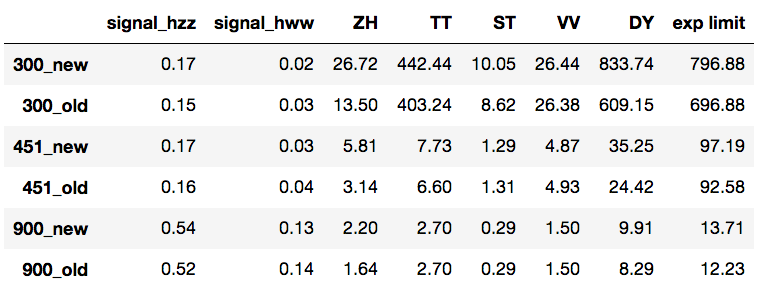
\includegraphics[width=0.91\textwidth]{ee_yields.png}
    \caption{Yields for ee channel before and after the tight isolation bug fix in the HEPPY. The effect is minimal as can be seen in the final limit. }
    \label{fig:yields_ee}
  \end{center}
\end{figure}



\subsection{Signal and background characteristics}

The signal region is further purified applying the cut in the BDT
output (Table ~\ref{EfficiencyBDT} contains the efficiency numbers for the BDT cut). 
The first set of BDT variables in the early version of the analysis included 30-50 variables, which could potentially discriminate signal from the background. The set containe\
d variables related to the kinematical properties of the signature, as well as a dozen of angular variables. After the first optimization, nine best variables were determined and chosen \
to be used for the analysis. Removal or addition of other variables did not improve the performance. %The same set of nine variables is used in both low and high mass trainings.


Following the procedure adopted by matured HH analyses, we
split the mass range into two: low mass and high mass (\`a la HIG-17-002 and HIG-17-008). These simplification costs some performance loss but allows analysis to proceed with just two BDTs instead of training one BDT per mass point, which would require more than a dozen of trainings per heavy resonance, though, training a dedicated BDT for each
signal mass hypothesis would give a better performance. However, the adopted path saves computational resources. Another reason is impracticality, bbZZ
signature is not the most sensitive, bb$\gamma$$\gamma$ is and the difference in sensitivity is a factor of 30-100 depending on the mass. More in the chapter \ref{sec:mva}.
%In addition, it would require a training of 16 BDTs per particle (BulkGraviton in our case). 
The low/high mass boundary value for HH analyses is chosen typically in the range 300-450
GeV. In our case the performance of the boundary around 300 GeV (area under the ROC curve
for low mass BDT is 0.9138 and 0.9805 for high mass BDT) is
similar to the boundary option at the 450 GeV (area under the ROC curve
for low mass BDT is 0.9086 and 0.9957 for high mass BDT), and to the one in the
middle of the range (area under the ROC curve
for 400 GeV for low mass BDT is 0.9074 and 0.9928 for high mass BDT). 
%https://indico.cern.ch/event/628835/contributions/2639777/attachments/1483653/2302207/Rami_HH_27June2017_v3.pdf
Therefore, we chose the value of 450 GeV, which
is also a choice of the bbbb analysis \cite{bbbb}. Upon running the full chain up to analysis limits, the choice of 450 GeV was confirmed to be the best split point option. As a result, the low
mass BDT includes a mix (with the weight '1') of seven signal samples:
250, 260, 270, 300, 350 400, 450 GeV. The high mass training includes nine
masses: 500, 550, 600, 650, 700, 750, 800, 900, 1000. In each case the
composition of the background is the same, it is a mix (by cross
section) of \ttbar and Drell-Yan plus jets.


Cut flow for ee and mm channels from the gen level up to before the BDT selection is shown on the figures ~\ref{fig:cutFlow}. In the cut flow table ~\ref{fig:cutFlow} the following definitions are used: very loose selection means all GsfElectrons and Muons from the basic collections that match gen-level electrons/muons and pass the very minimal kinematic cuts; loose selection means loose POG selection consisting of kinematic, dxy/dz, iso cuts. The final efficiency values represent these numbers in terms of events ~\ref{cutFlowEvents}:

\begin{table}
\begin{center}
\caption{Number of events surviving analysis cuts corresponding to the last entry in the ~\ref{fig:cutFlow} .}
\begin{tabular}{|c|c|c|} \hline
{Process, mass point} &  ee channel, \% &  mm channel, \% \\\hline
bbZZ, 300 GeV &                    2256     &                    4511 \\
bbWW, 300 GeV &                    53       &                    85 \\
bbZZ, 900 GeV &                    8034     &                    12963 \\
bbWW, 900 GeV &                    12       &                    23 \\\hline
\end{tabular}
\label{cutFlowEvents}
\end{center}
\end{table}






\subsubsection{Data and MC comparison\label{sec:compareDataMC}}
Signal region BDT side-band plots as well as unblind signal region plots show good data-MC agreements.
We are not cutting on BDT for control regions, therefore, all the mass
point have the same background and data distributions. 
That is
why we provide below plots for two mass points: one mass point representing low mass region, 300 GeV, and one mass point representing high mass region, 900 geV. 
% for other pass point only signal distribution will change,
%however, data/background comparison and their ratio will not. At the same time, BDT outputs are mass point specific, because are trained for two different mass regions - low and high mass regions, and are evaluated for each mass point separately. Thus, we show all the BDT plots. 
Signal bbZZ and bbWW rates for all plots are multiplied by some high factors depending on the mass point purely for the visualization purpose and do not go in the real analysis. 

Prefit plots are available in the Appendix ~\ref{sec:datamc}. Control regions only postfit plots have been produced during an extensive discussion with Higgs conveners at HyperNews, and it was shows that upon inclusion of the SR in the fit the data-MC agreement is slightly better. Postfit plots that include SR in simultaneous fit, hence a common jargon name ``Full postfit`` plots, are presented at the figures ~\ref{fig:MCcomparison_mm_300} - ~\ref{fig:MCcomparison_ee_900} and show data and MC comparison in the SR, CRDY, and CRTT. For both ee and mm channels, low and high mass regions. The latest style plots produced for the PAS can be found at Fig.~\ref{fig:MCcomparisons} for the graviton case and Fig.~\ref{fig:MCcomparisons_radion} for the radion case. 



Distributions of nine variables that go into the BDT have been studied in depth during the pre-approval process and are available in the Appendix ~\ref{sec:datamc}. After the tight isolation cut fix in the HEPPY framework the results/shapes are almost unchanged (it is also can be observed from the table of yields ~\ref{fig:yields_ee}).  At the yields table ~\ref{fig:yields_ee}, 450 GeV mass point, since evaluated using the high mass BDT, is called 451 GeV for clarity purposes. 



\begin{figure}[tbp]
  \begin{center}
    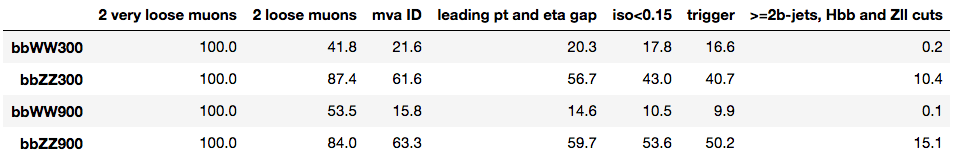
\includegraphics[width=0.91\textwidth]{cutflow_mm.png}\\
    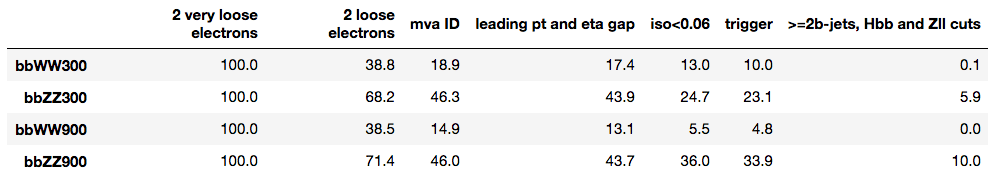
\includegraphics[width=0.91\textwidth]{cutflow_ee.png}\\
    \caption{Cut flow for mm (top) and ee (bottom) channels. }
    \label{fig:cutFlow}
  \end{center}
\end{figure}



%% \begin{figure}[tbp]                                                                                                                                           
%%   \begin{center}                                                                                                                                              
%%     \includegraphics[width=0.31\textwidth]{mm_300_july20/hhMt_mm_SR_FullPostfit_plot_july20.png}                                                  
%%     \includegraphics[width=0.31\textwidth]{mm_300_july20/hhMt_mm_CRDY_FullPostfit_plot_july20.png}
%%     \includegraphics[width=0.31\textwidth]{mm_300_july20/hhMt_mm_CRTT_FullPostfit_plot_july20.png}\\                                              
%%     \includegraphics[width=0.31\textwidth]{mm_300_july20/bdt_response_mm_SR_FullPostfit_plot_july20.png}                                         
%%     \includegraphics[width=0.31\textwidth]{mm_300_july20/bdt_response_mm_CRDY_FullPostfit_plot_july20.png}                                           
%%     \includegraphics[width=0.31\textwidth]{mm_300_july20/bdt_response_mm_CRTT_FullPostfit_plot_july20.png}\\                                
%%     \caption{Comparison of data and MC samples. 300 GeV, mm channel, Full Postfit plots. Top: hhMt, bottom: BDT distributions. From left to right: SR, CRDY, CRTT.}
%%     \label{fig:MCcomparison_mm_300}                                                                                                                   
%%   \end{center}                                                                                                                                                
%% \end{figure}                                                                                                                                                  


%% \begin{figure}[tbp]                                                                                                                                           
%%   \begin{center}                                                                                                                                              
%%     \includegraphics[width=0.31\textwidth]{ee_300_july20/hhMt_ee_SR_FullPostfit_plot_july20.png}                                                  
%%     \includegraphics[width=0.31\textwidth]{ee_300_july20/hhMt_ee_CRDY_FullPostfit_plot_july20.png}
%%     \includegraphics[width=0.31\textwidth]{ee_300_july20/hhMt_ee_CRTT_FullPostfit_plot_july20.png}\\                                              
%%     \includegraphics[width=0.31\textwidth]{ee_300_july20/bdt_response_ee_SR_FullPostfit_plot_july20.png}                                         
%%     \includegraphics[width=0.31\textwidth]{ee_300_july20/bdt_response_ee_CRDY_FullPostfit_plot_july20.png}                                           
%%     \includegraphics[width=0.31\textwidth]{ee_300_july20/bdt_response_ee_CRTT_FullPostfit_plot_july20.png}\\                                
%%     \caption{Comparison of data and MC samples. 300 GeV, ee channel, Full Postfit plots. Top: hhMt, bottom: BDT distributions. From left to right: SR, CRDY, CRTT.}
%%     \label{fig:MCcomparison_ee_300}                                                                                                                   
%%   \end{center}                                                                                                                                                
%% \end{figure}                                                                                                                                                  




%% \begin{figure}[tbp]                                                                                                                                           
%%   \begin{center}                                                                                                                                              
%%     \includegraphics[width=0.31\textwidth]{mm_900_july20/hhMt_mm_SR_FullPostfit_plot_july20.png}                                                  
%%     \includegraphics[width=0.31\textwidth]{mm_900_july20/hhMt_mm_CRDY_FullPostfit_plot_july20.png}
%%     \includegraphics[width=0.31\textwidth]{mm_900_july20/hhMt_mm_CRTT_FullPostfit_plot_july20.png}\\                                              
%%     \includegraphics[width=0.31\textwidth]{mm_900_july20/bdt_response_mm_SR_FullPostfit_plot_july20.png}                                         
%%     \includegraphics[width=0.31\textwidth]{mm_900_july20/bdt_response_mm_CRDY_FullPostfit_plot_july20.png}                                           
%%     \includegraphics[width=0.31\textwidth]{mm_900_july20/bdt_response_mm_CRTT_FullPostfit_plot_july20.png}\\                                
%%     \caption{Comparison of data and MC samples. 900 GeV, mm channel, Full Postfit plots. Top: hhMt, bottom: BDT distributions. From left to right: SR, CRDY, CRTT.}
%%     \label{fig:MCcomparison_mm_900}                                                                                                                   
%%   \end{center}                                                                                                                                                
%% \end{figure}                                                                                                                                                  


%% \begin{figure}[tbp]                                                                                                                                           
%%   \begin{center}                                                                                                                                              
%%     \includegraphics[width=0.31\textwidth]{ee_900_july20/hhMt_ee_SR_FullPostfit_plot_july20.png}                                                  
%%     \includegraphics[width=0.31\textwidth]{ee_900_july20/hhMt_ee_CRDY_FullPostfit_plot_july20.png}
%%     \includegraphics[width=0.31\textwidth]{ee_900_july20/hhMt_ee_CRTT_FullPostfit_plot_july20.png}\\                                              
%%     \includegraphics[width=0.31\textwidth]{ee_900_july20/bdt_response_ee_SR_FullPostfit_plot_july20.png}                                         
%%     \includegraphics[width=0.31\textwidth]{ee_900_july20/bdt_response_ee_CRDY_FullPostfit_plot_july20.png}                                           
%%     \includegraphics[width=0.31\textwidth]{ee_900_july20/bdt_response_ee_CRTT_FullPostfit_plot_july20.png}\\                                
%%     \caption{Comparison of data and MC samples. 900 GeV, ee channel, Full Postfit plots. Top: hhMt, bottom: BDT distributions. From left to right: SR, CRDY, CRTT.}
%%     \label{fig:MCcomparison_ee_900}                                                                                                                   
%%   \end{center}                                                                                                                                                
%% \end{figure}                                                                                                                                                  

\begin{figure}[tbp]
  \begin{center}
    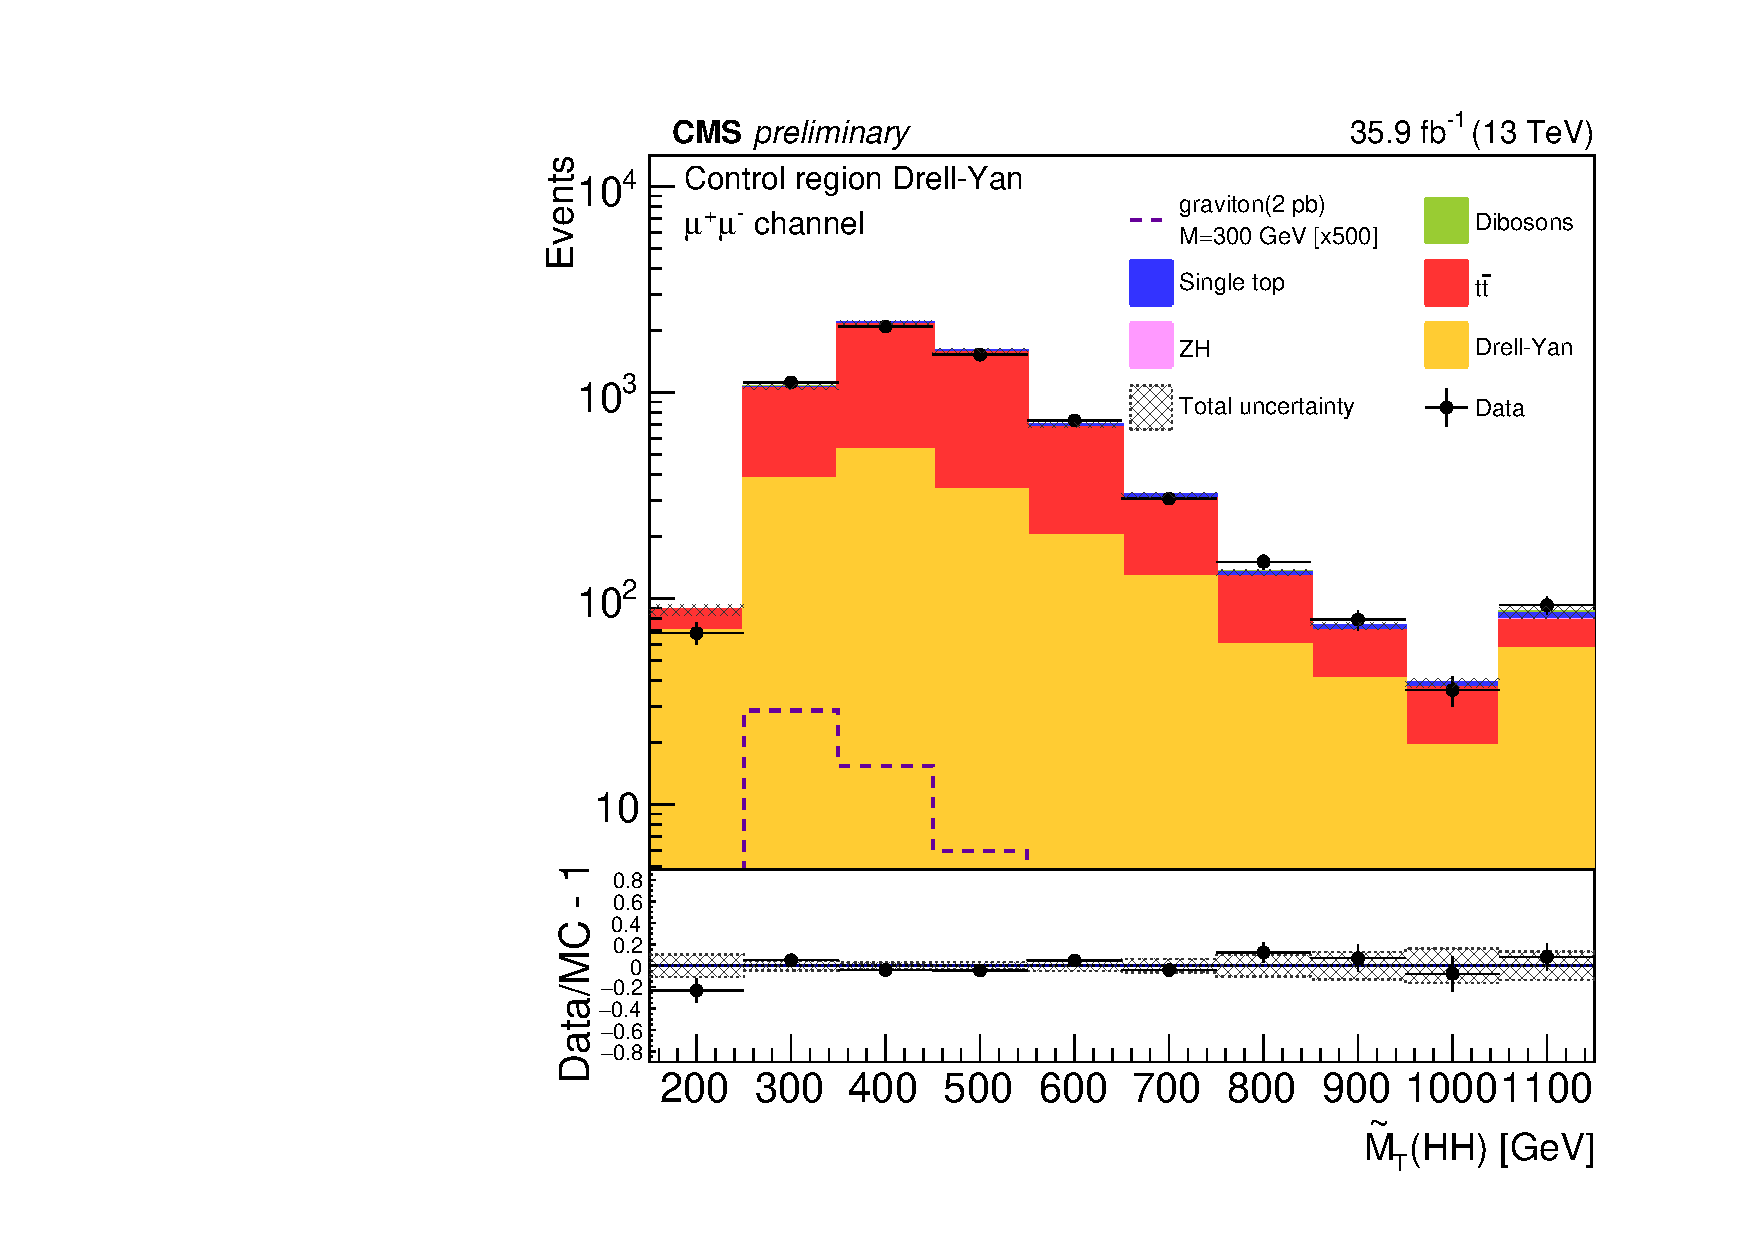
\includegraphics[width=0.31\textwidth]{hhMt_mm_CRDY_FullPostfit_plot_nov16_2_graviton.pdf}
    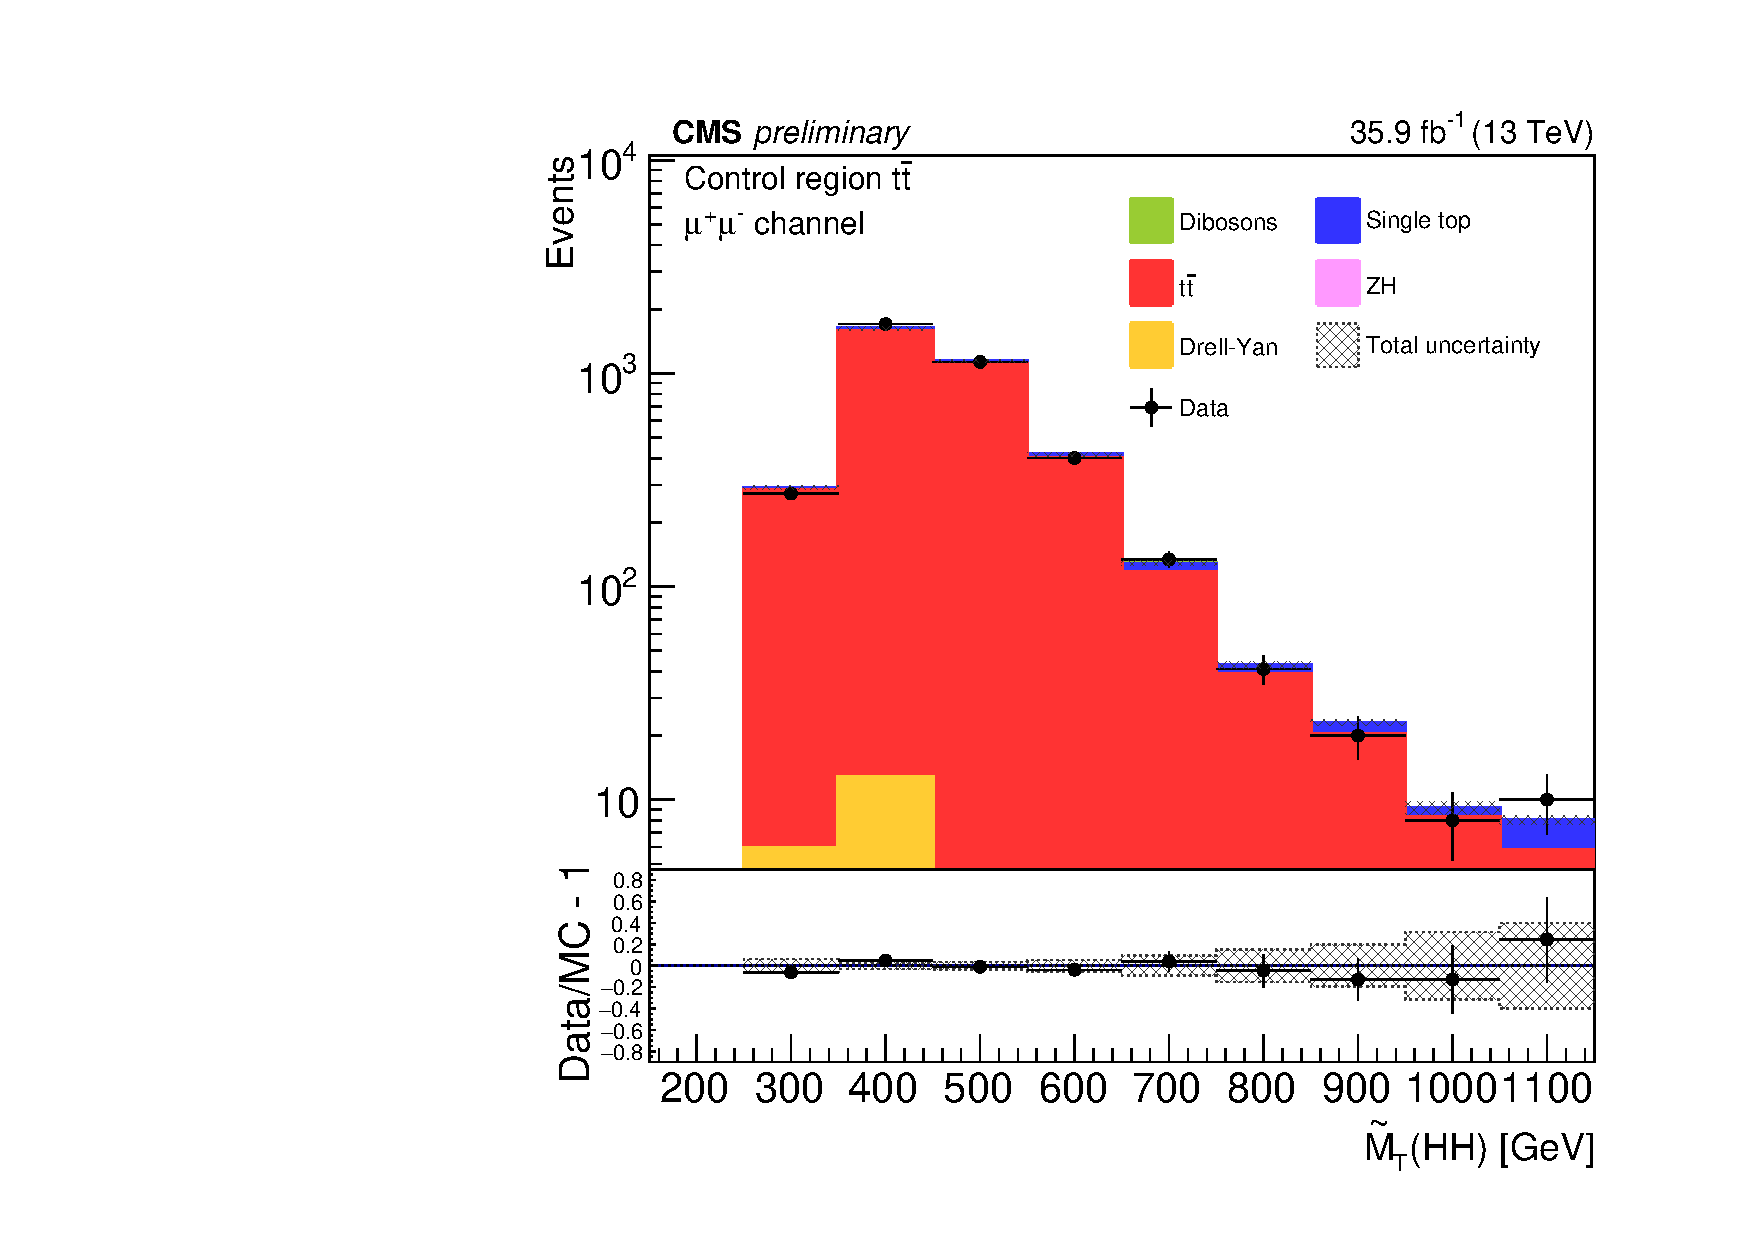
\includegraphics[width=0.31\textwidth]{hhMt_mm_CRTT_FullPostfit_plot_nov16_2_graviton.pdf}
    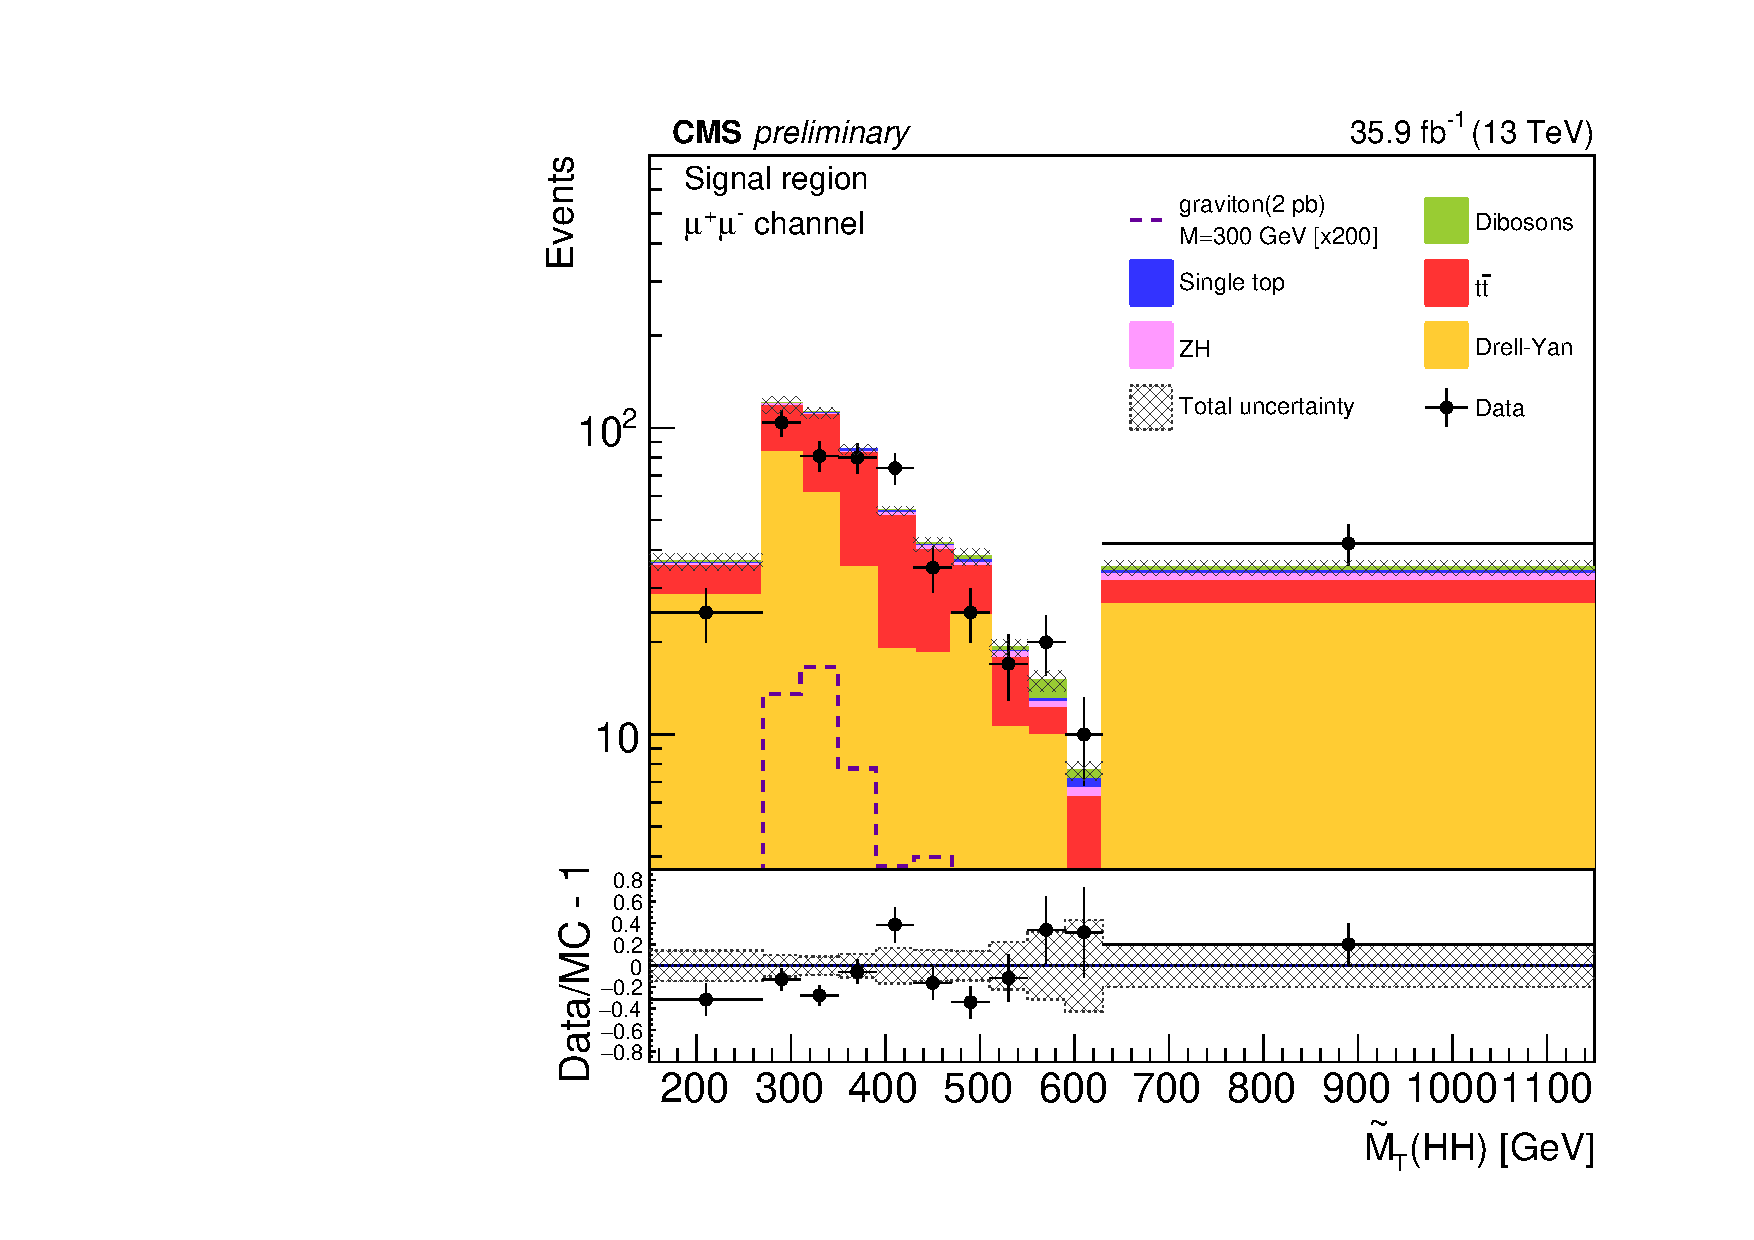
\includegraphics[width=0.31\textwidth]{hhMt_mm_SR_FullPostfit_plot_nov16_2_graviton.pdf} \\
    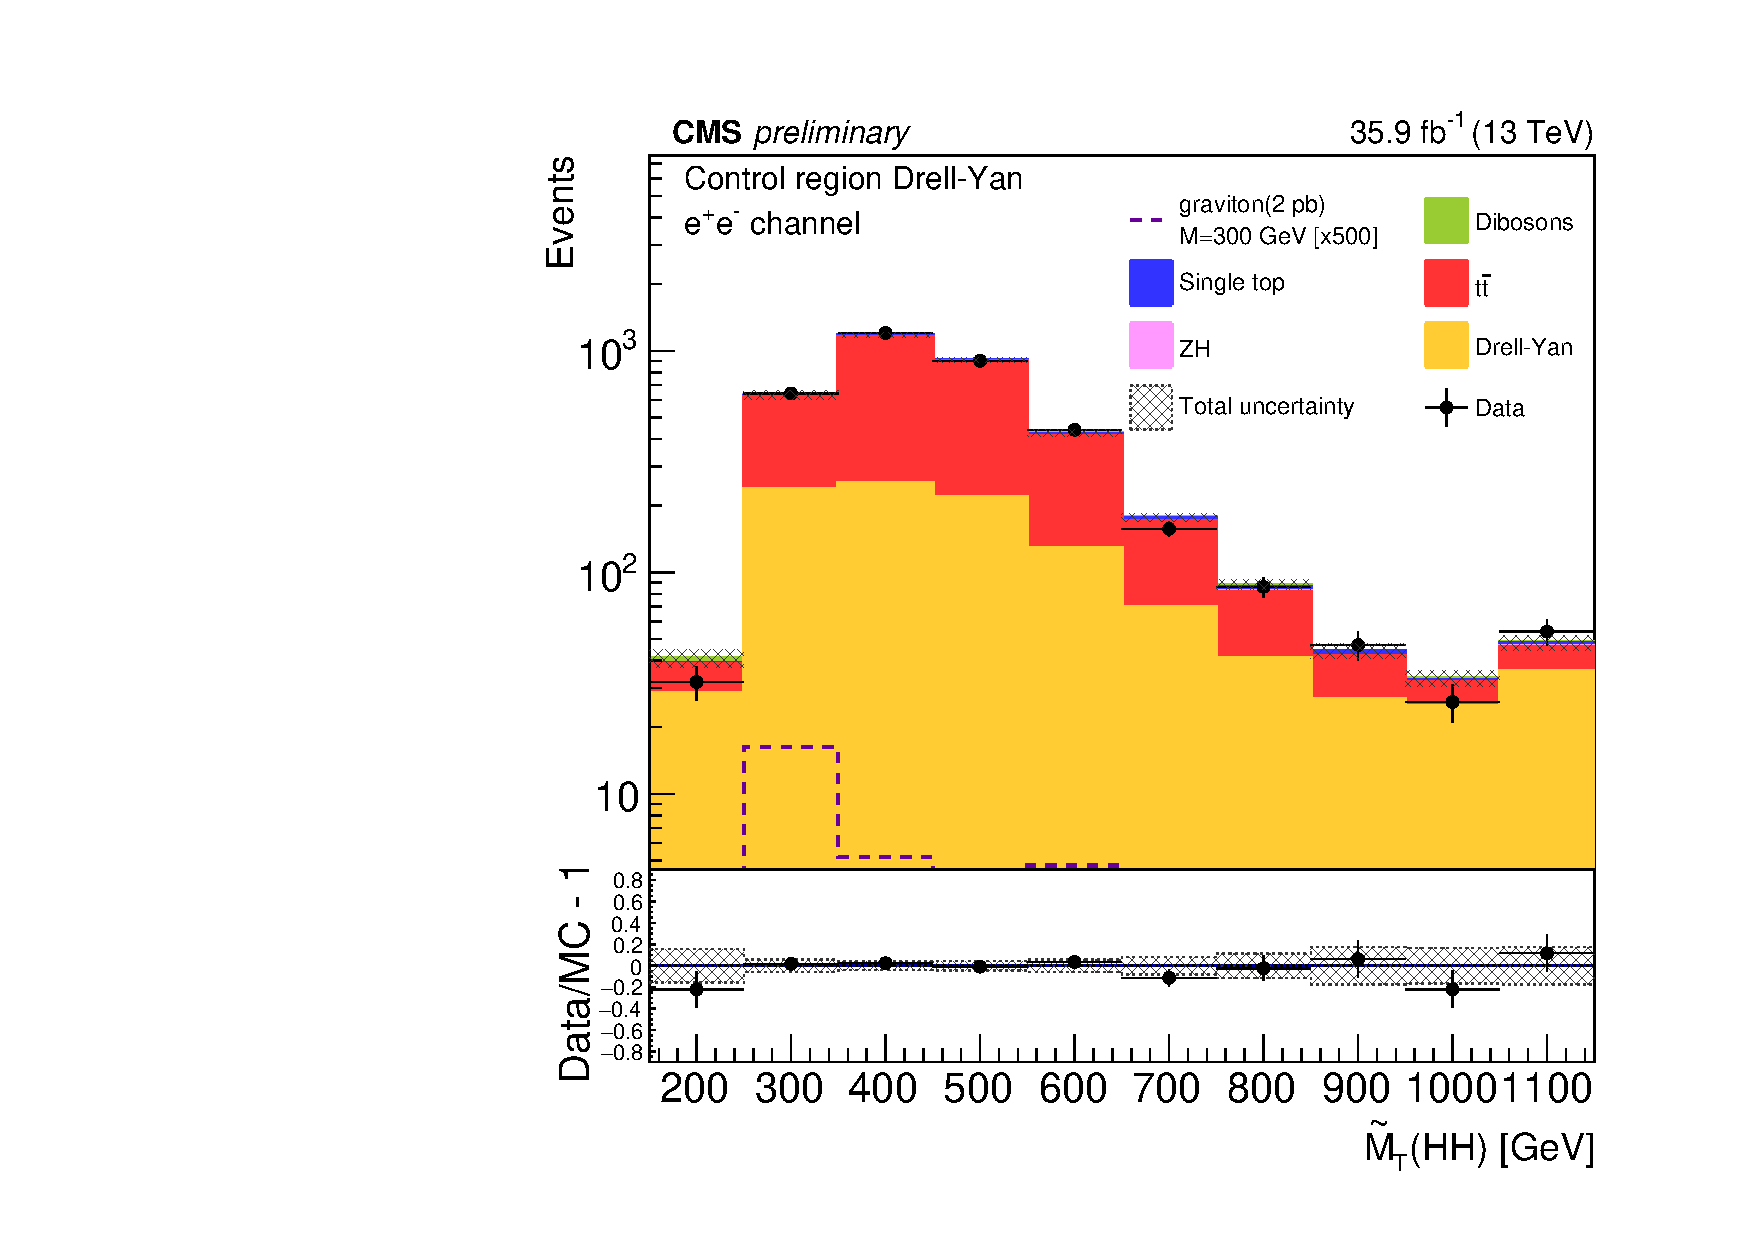
\includegraphics[width=0.31\textwidth]{hhMt_ee_CRDY_FullPostfit_plot_nov16_2_graviton.pdf}
    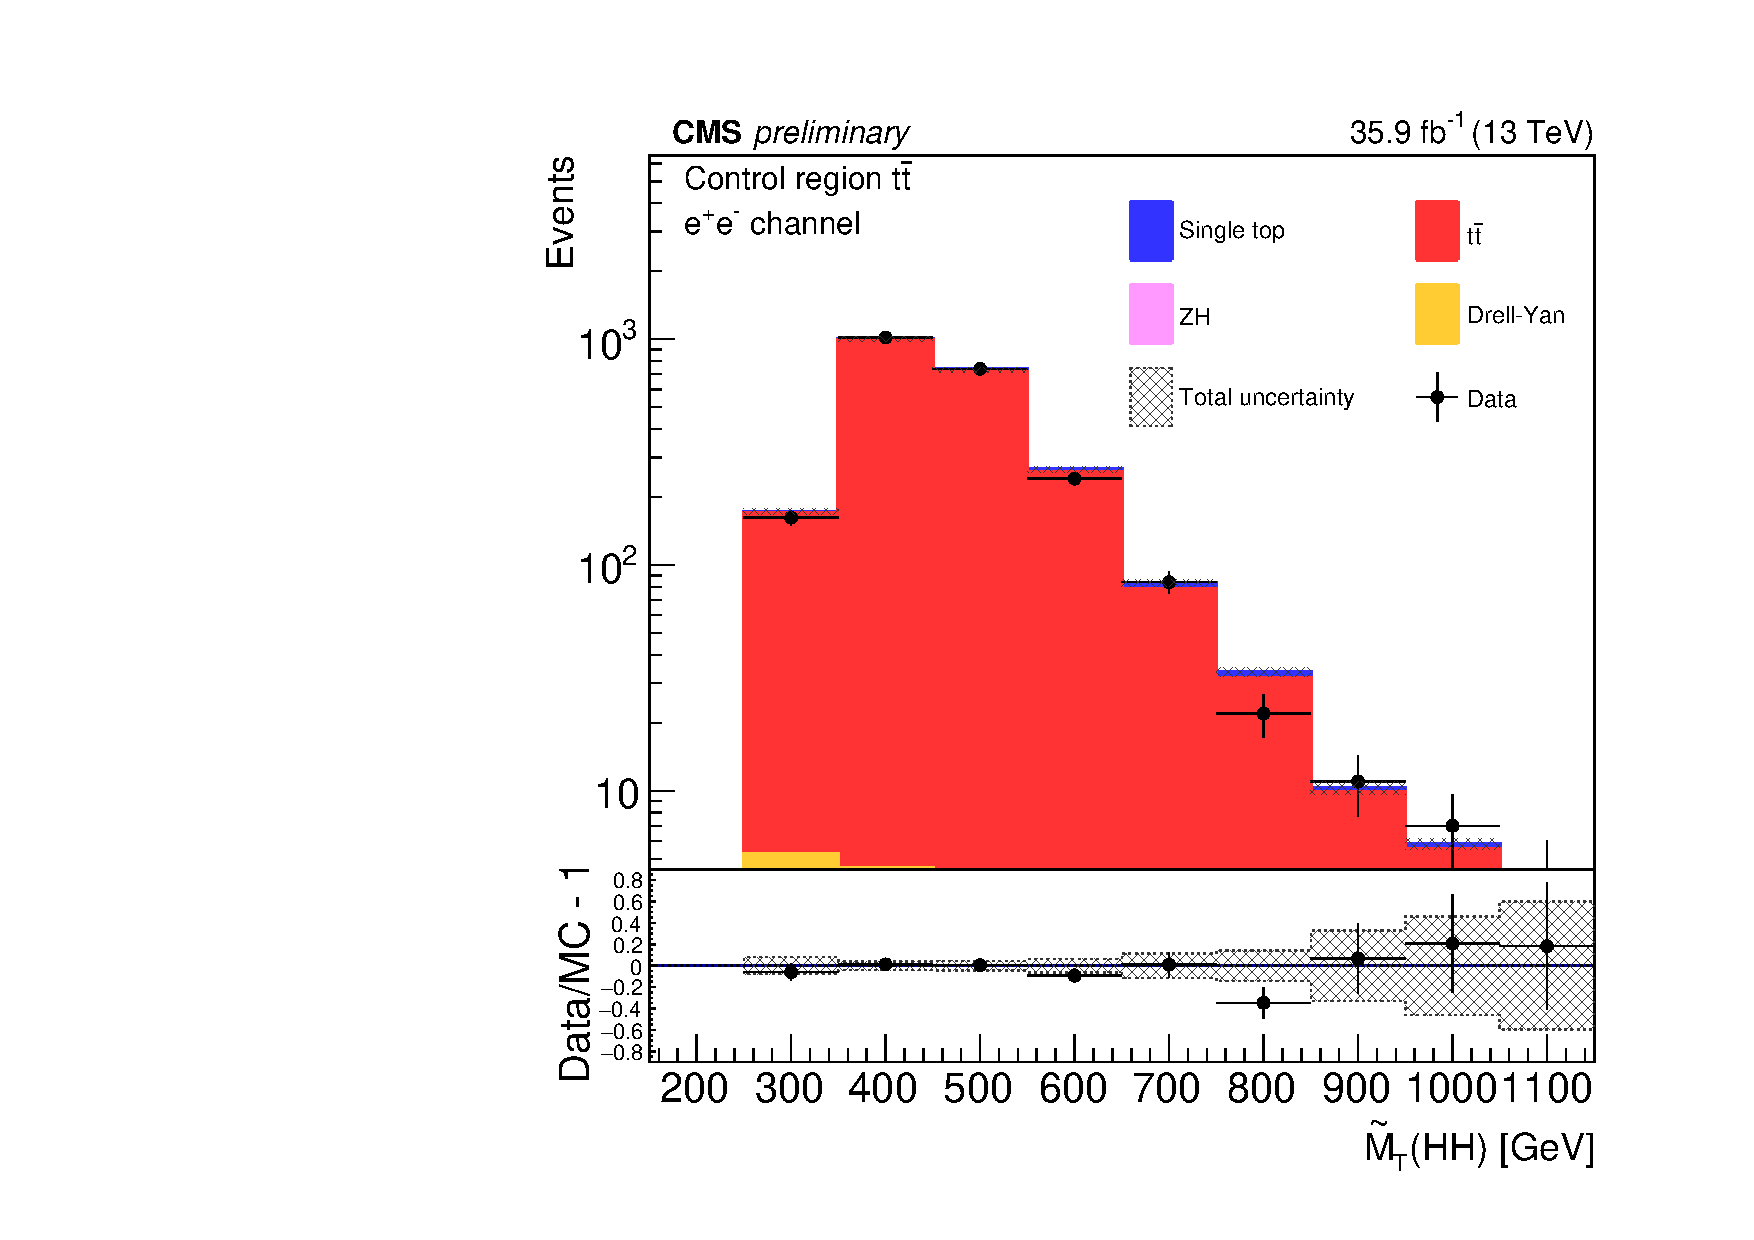
\includegraphics[width=0.31\textwidth]{hhMt_ee_CRTT_FullPostfit_plot_nov16_2_graviton.pdf}
    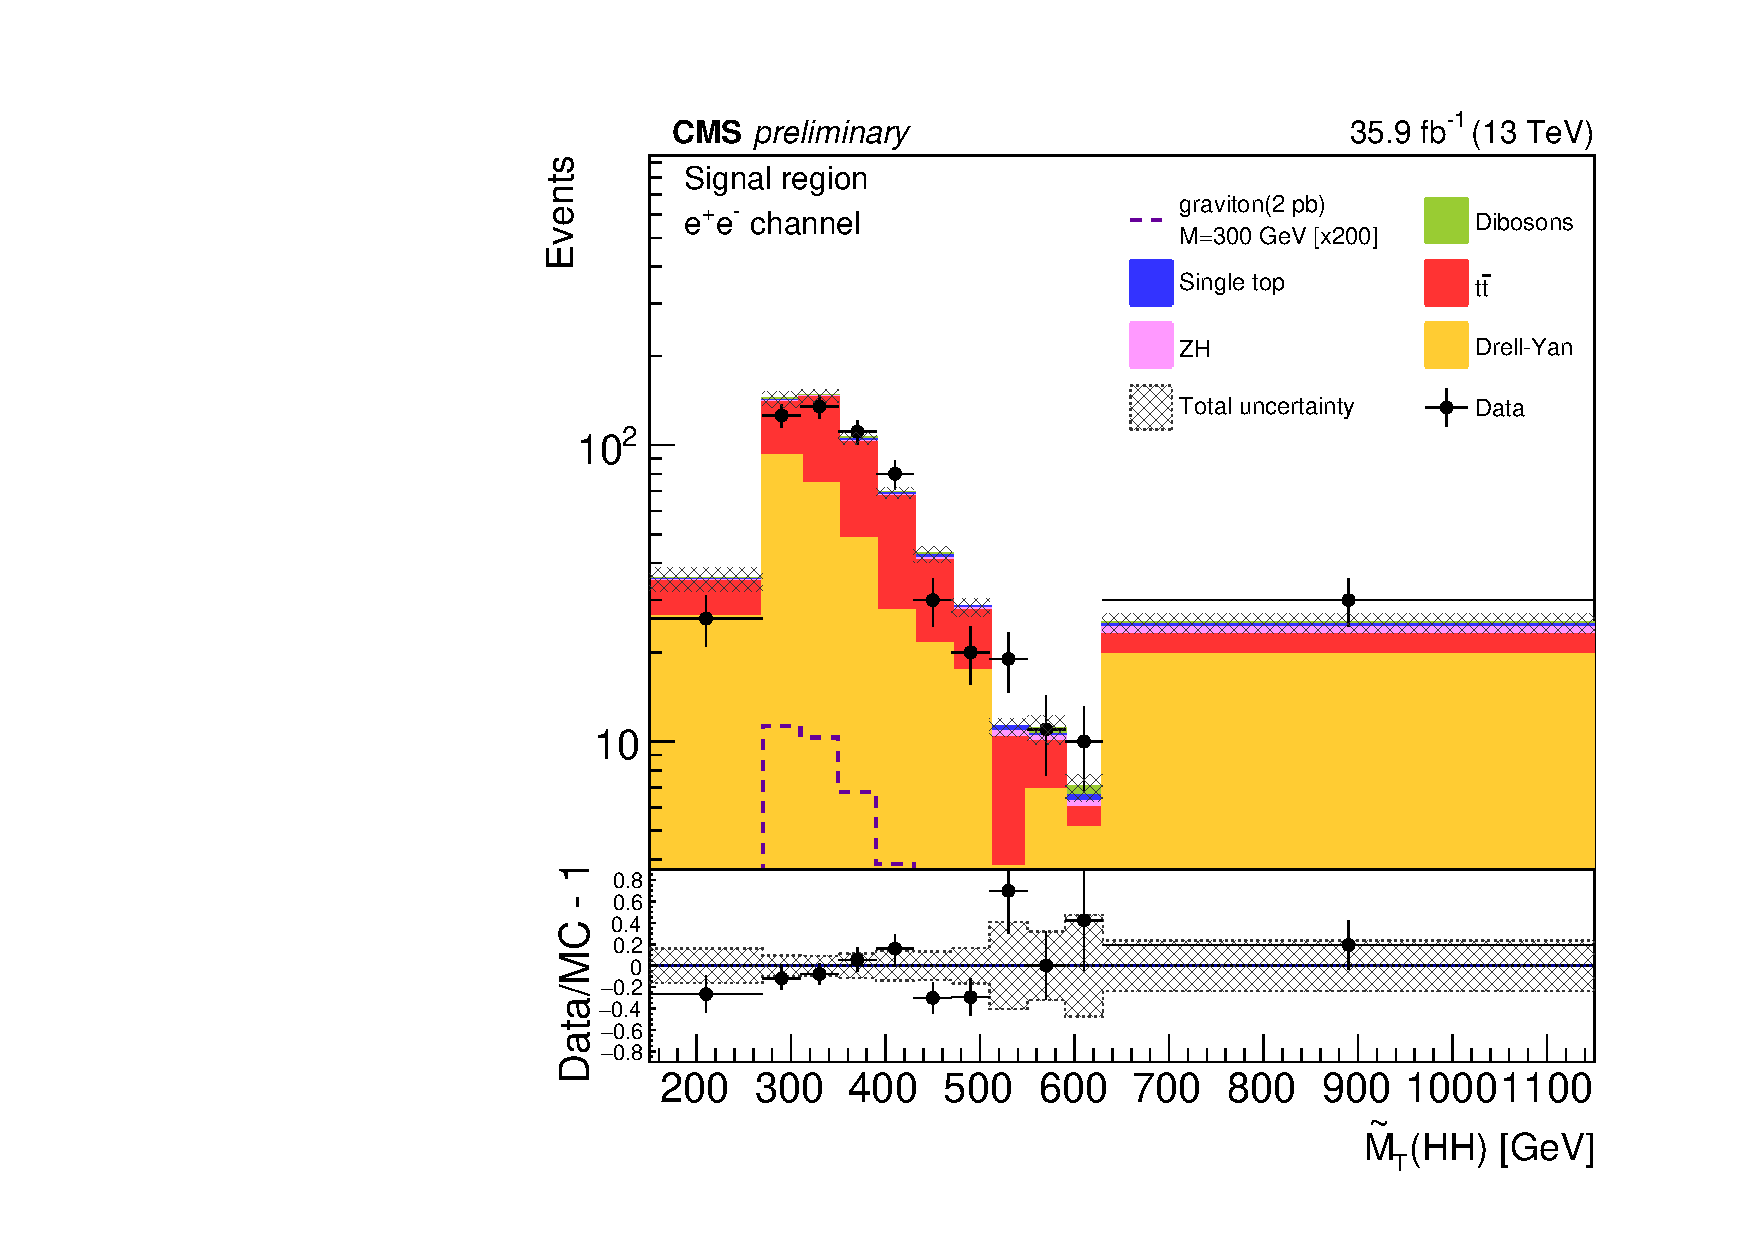
\includegraphics[width=0.31\textwidth]{hhMt_ee_SR_FullPostfit_plot_nov16_2_graviton.pdf}
    \caption{Transverse mass of the reconstructed HH candidates for data, the simulated signal graviton sample
    for the 300 GeV mass hypothesis, and simulated backgrounds scaled according to the fit results. The top
    row shows the figures for the muon channel while the bottom row is for the electron channel. For each row,
    the left plot is for the Drell-Yan control region, the middle is for the \ttbar control region, and the right
    is for the signal region. Signal normalization choice is discussed in the text. The crosshatched area represe\
nts
    the sum of statistical and systematic uncertainties.}
    \label{fig:MCcomparisons}
%                                                                                                                 
% Comparison of data and simulation.  Transverse mass of                                                          
%      the reconstructed HH candidate for 300 GeV signal mass                                                     
%      hypothesis, electron channel. Left: Drell-Yan control region. Middle: \ttbar                               
%      control region. Right: signal region. }                                                                    
%    \label{MCcomparisons_electrons}                                                                              
  \end{center}
\end{figure}




\begin{figure}[tbp]
  \begin{center}
    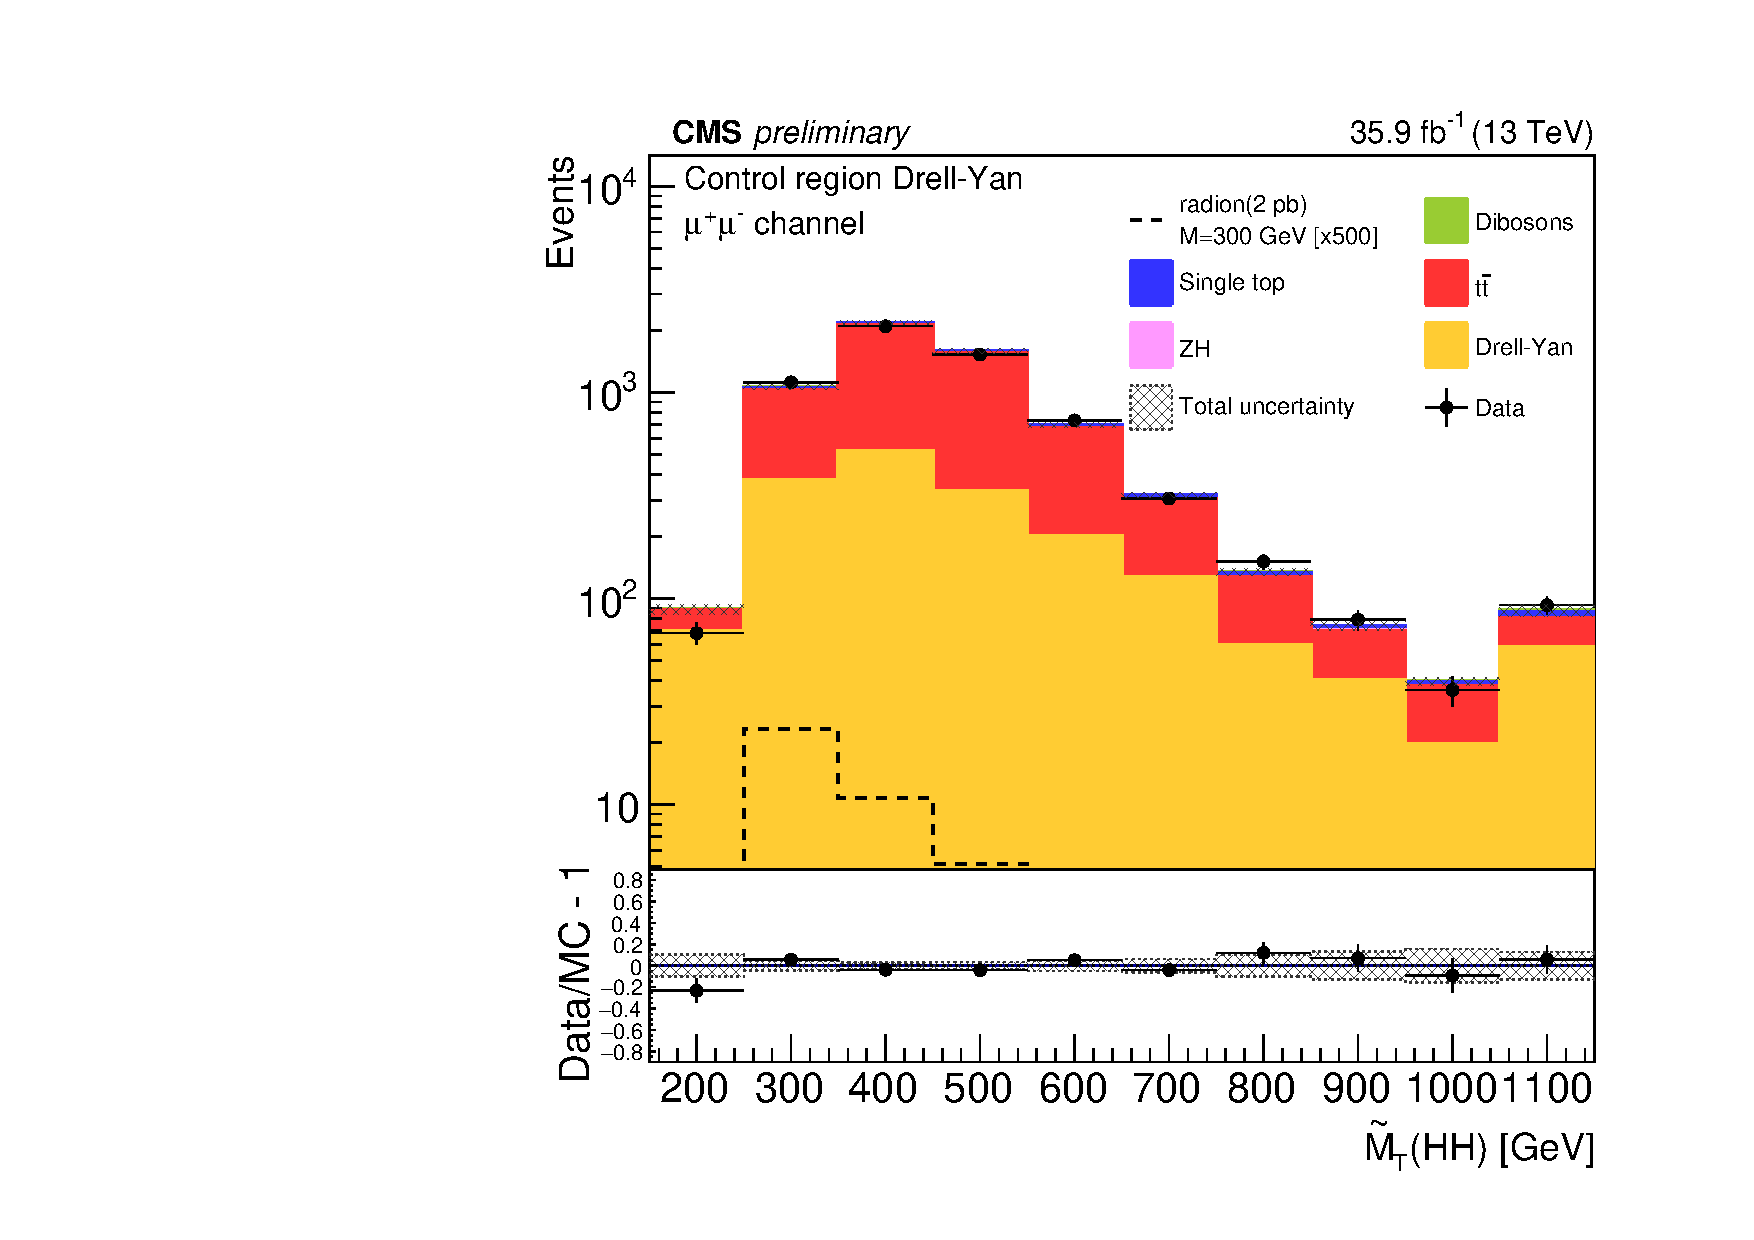
\includegraphics[width=0.31\textwidth]{hhMt_mm_CRDY_FullPostfit_plot_nov16_2_radion.pdf}
    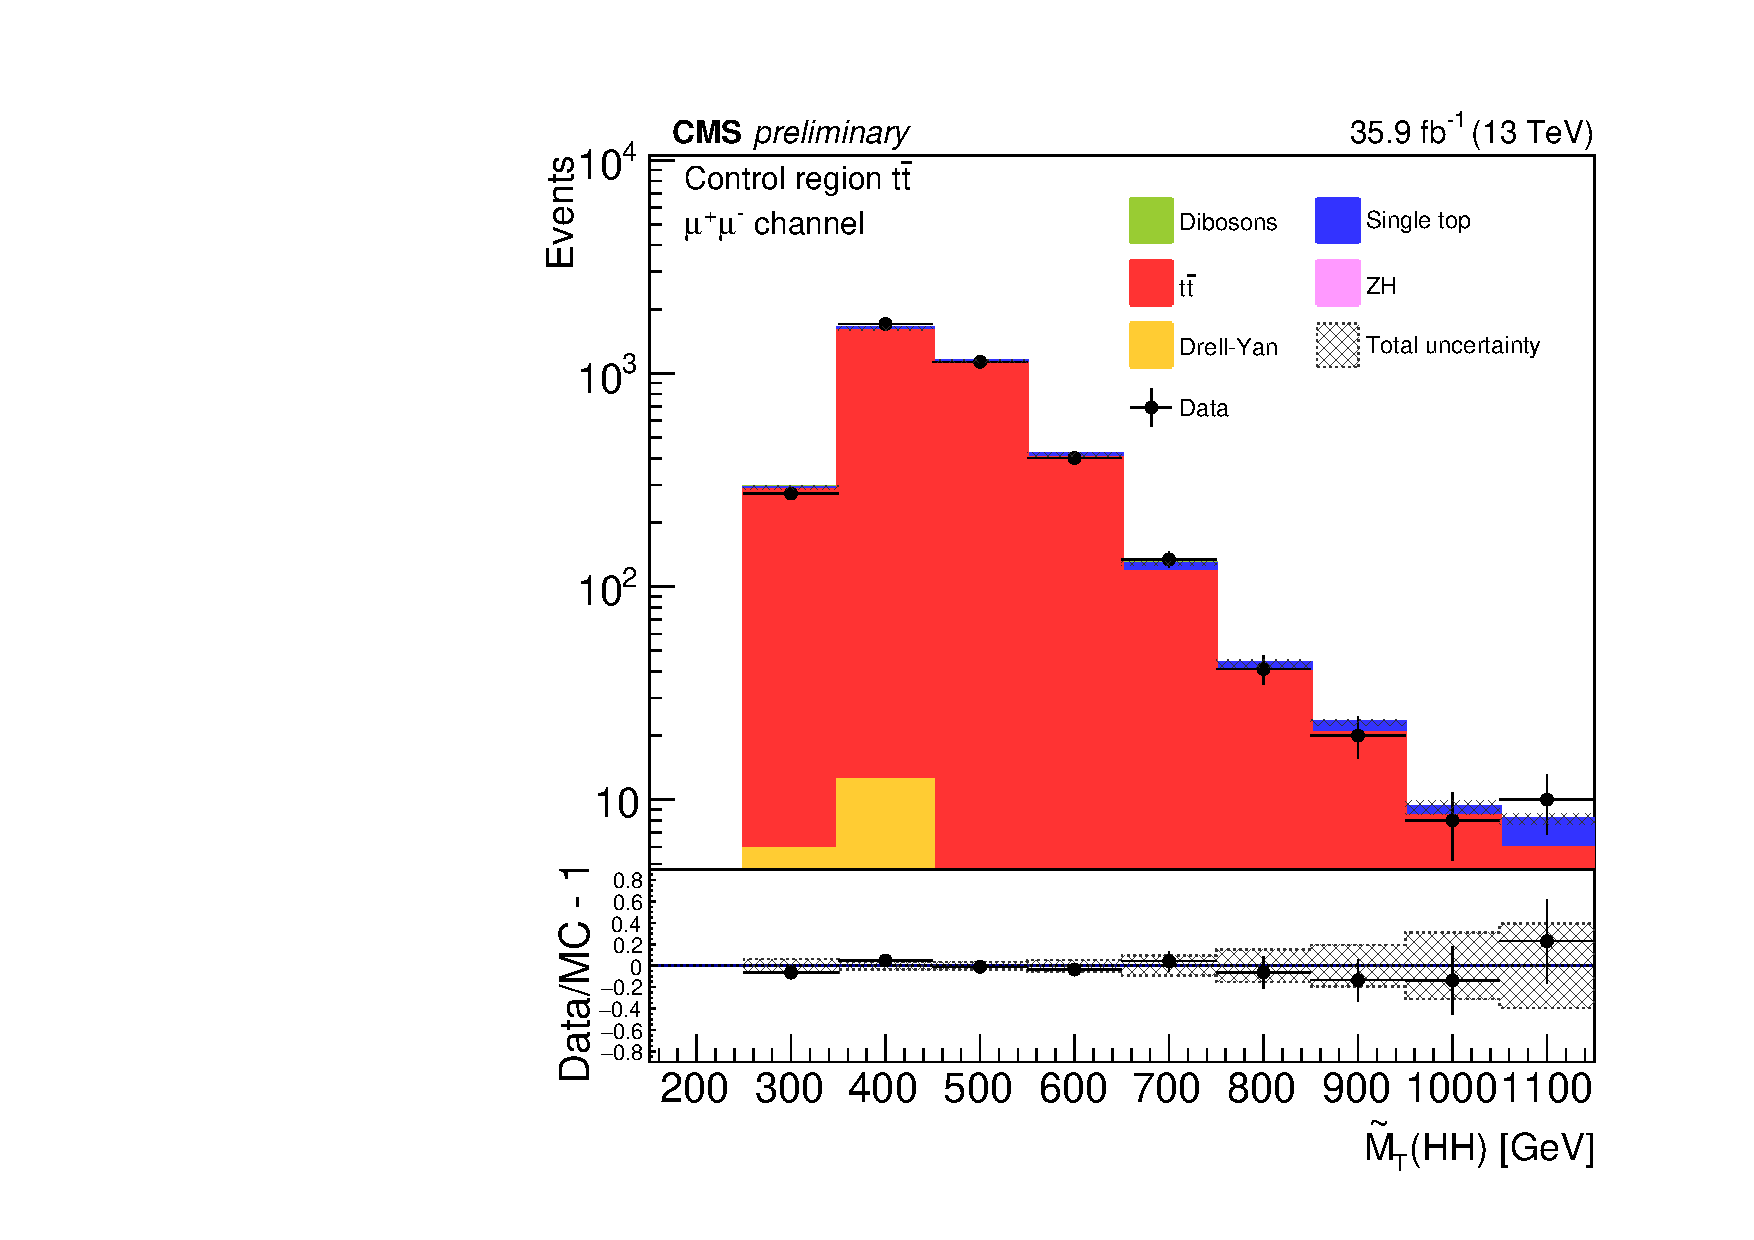
\includegraphics[width=0.31\textwidth]{hhMt_mm_CRTT_FullPostfit_plot_nov16_2_radion.pdf}
    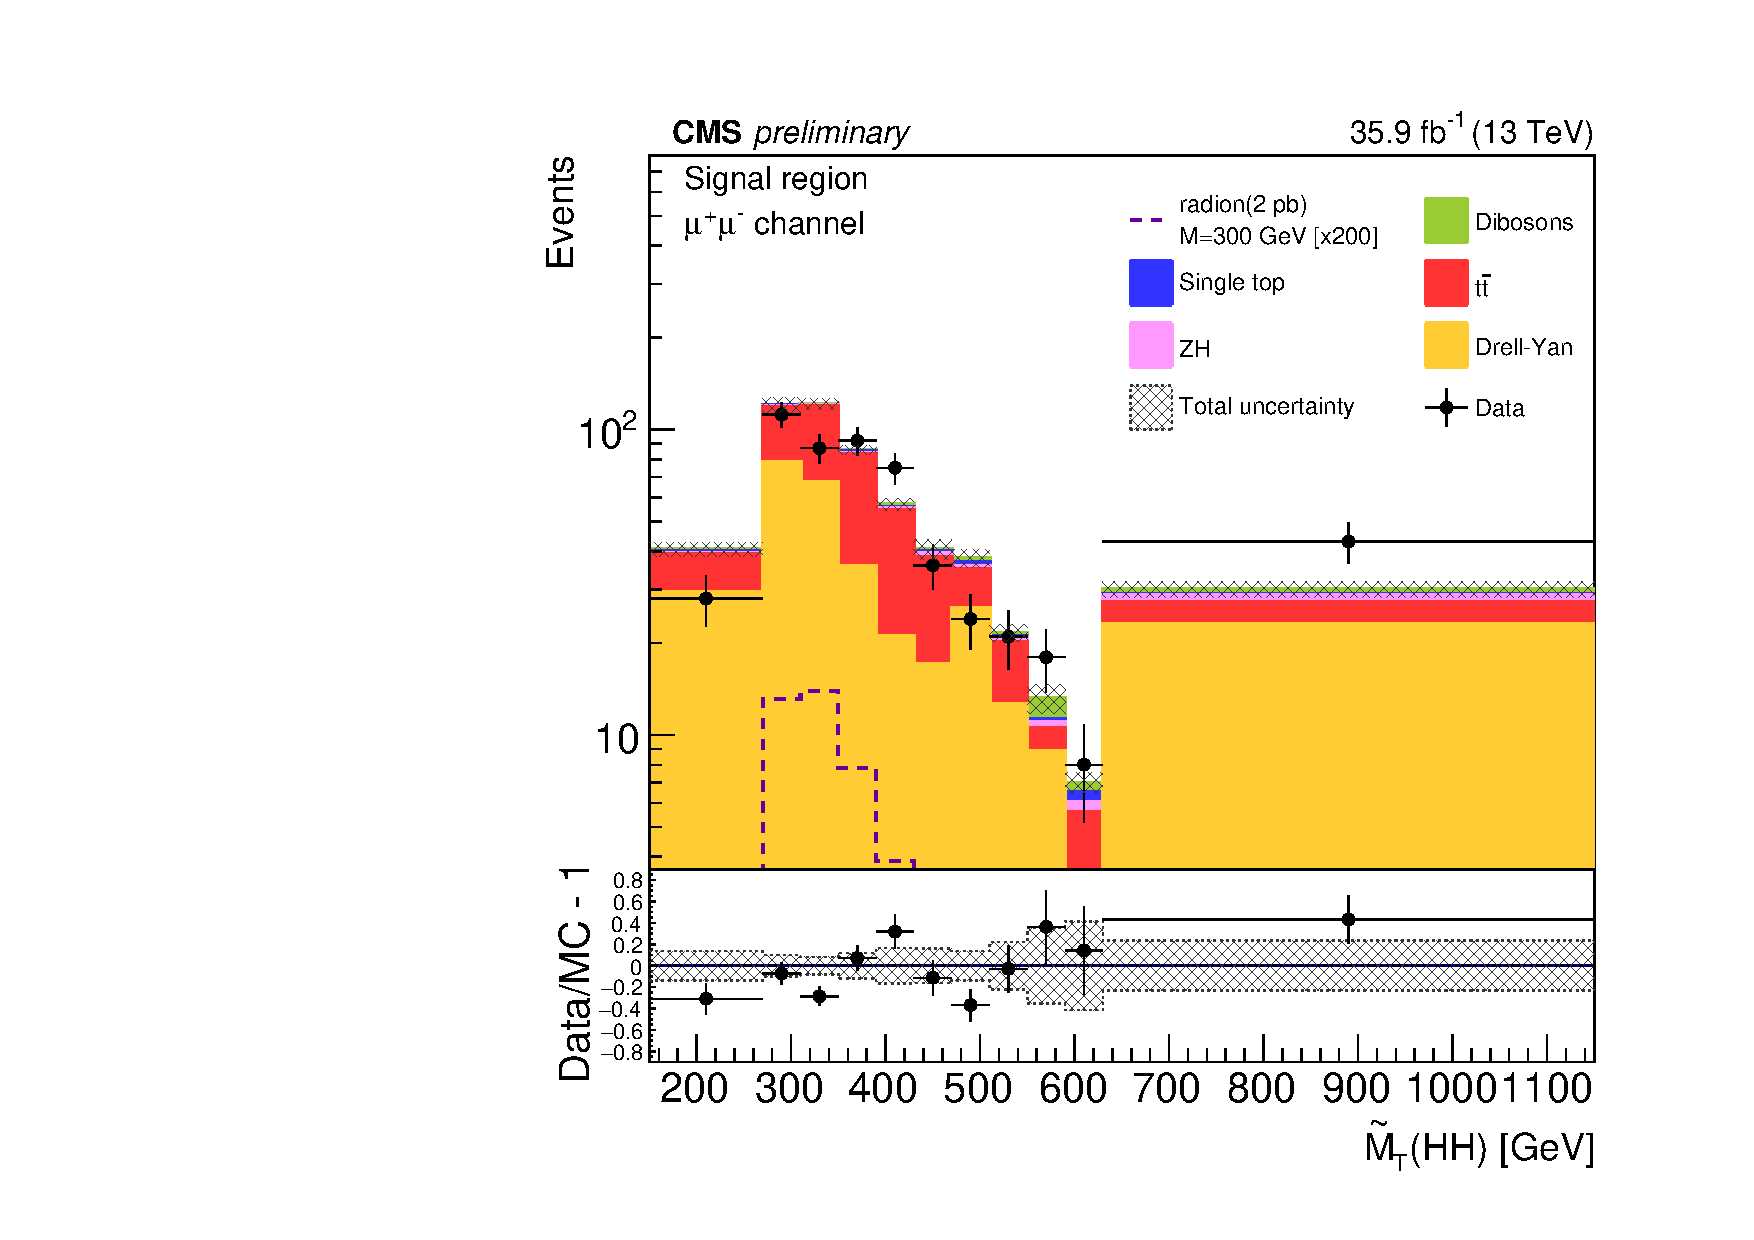
\includegraphics[width=0.31\textwidth]{hhMt_mm_SR_FullPostfit_plot_nov16_2_radion.pdf} \\
    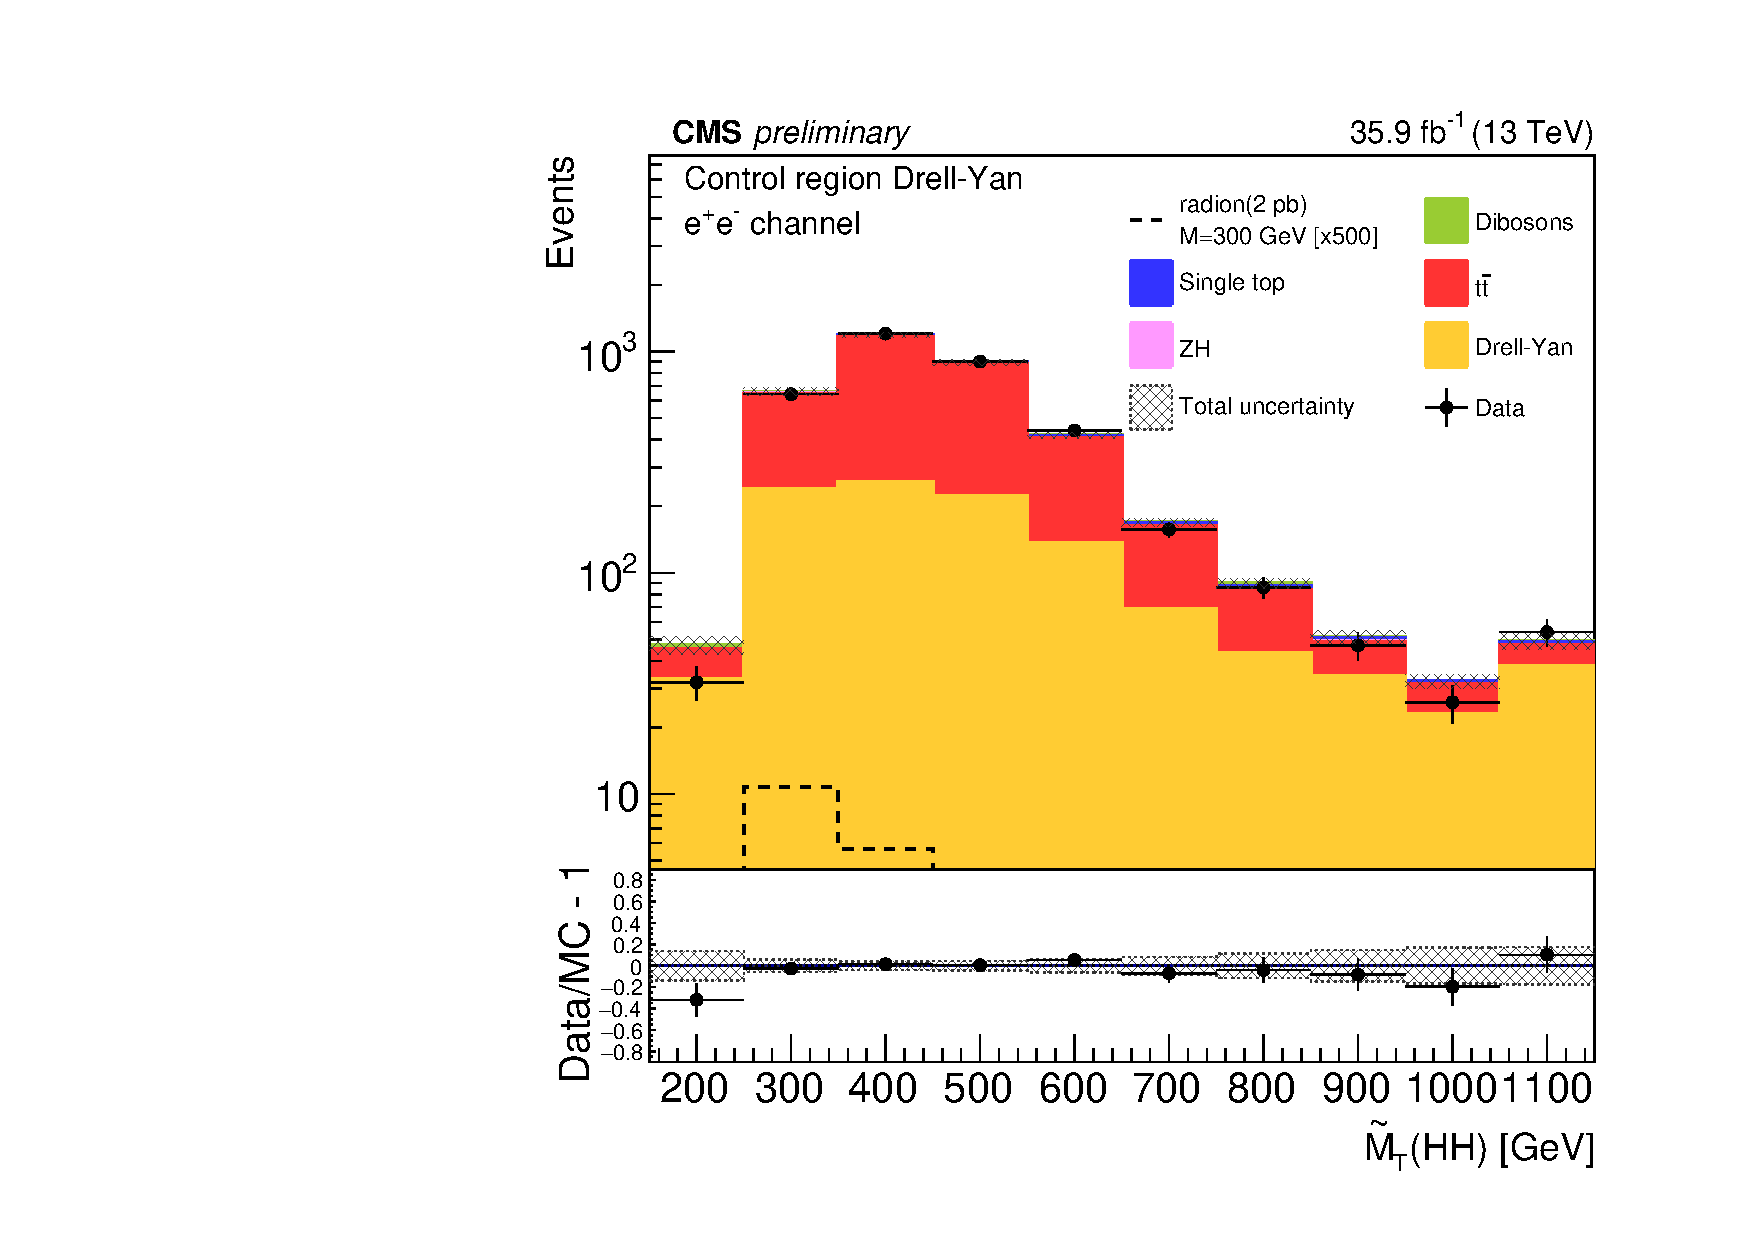
\includegraphics[width=0.31\textwidth]{hhMt_ee_CRDY_FullPostfit_plot_nov16_2_radion.pdf}
    \includegraphics[width=0.31\textwidth]{hhMt_ee_CRTT_FullPostfit_plot_nov16_2_radion.pdf}
    \includegraphics[width=0.31\textwidth]{hhMt_ee_SR_FullPostfit_plot_nov16_2_radion.pdf}
    \caption{Transverse mass of the reconstructed HH candidates for data, the simulated signal radion sample
    for the 300 GeV mass hypothesis, and simulated backgrounds scaled according to the fit results. The top
    row shows the figures for the muon channel while the bottom row is for the electron channel. For each row,
    the left plot is for the Drell-Yan control region, the middle is for the \ttbar control region, and the right
    is for the signal region. Signal normalization choice is discussed in the text. The crosshatched area represe\
nts
    the sum of statistical and systematic uncertainties.}
    \label{fig:MCcomparisons_radion}
%                                                                                                                 
% Comparison of data and simulation.  Transverse mass of                                                          
%      the reconstructed HH candidate for 300 GeV signal mass                                                     
%      hypothesis, electron channel. Left: Drell-Yan control region. Middle: \ttbar                               
%      control region. Right: signal region. }                                                                    
%    \label{MCcomparisons_electrons}                                                                              
  \end{center}
\end{figure}





%are presented (See Figs.  ~\ref{fig:MCcomparisons_ee_low_SR_bdt_sideband}, ~\ref{fig:MCcomparisons_ee_low_SR_bdt_sideband_2}, ~\ref{fig:MCcomparisons_ee_low_CRDY}, ~\ref{fig:MCcomparisons_ee_low_CRDY_2}, ~\ref{fig:MCcomparisons_ee_low_CRTT}, ~\ref{fig:MCcomparisons_ee_low_CRTT_2} . Unblinded ee distributions are shown in the Fig. ~\ref{fig:MCcomparisons_ee_low_SR}, ~\ref{fig:MCcomparisons_ee_low_SR_2}.
%Muon channel plots are also shown.(See Figs. ~\ref{fig:MCcomparisons_mm_low_SR_bdt_sideband}, ~\ref{fig:MCcomparisons_mm_low_SR_bdt_sideband_2}, ~\ref{fig:MCcomparisons_mm_low_CRDY}, ~\ref{fig:MCcomparisons_mm_low_CRDY_2}, ~\ref{fig:MCcomparisons_mm_low_CRTT}, ~\ref{fig:MCcomparisons_mm_low_CRTT_2}.  Unblinded mm distributions are shown in the Fig. ~\ref{fig:MCcomparisons_mm_low_SR}, ~\ref{fig:MCcomparisons_mm_low_SR_2}.

%BDT plots for all mass hypotheses for SR can be found on the Fig. ~\ref{fig:bdt_ee_SR} for electron channel and ~\ref{fig:bdt_mm_SR} for the muon channel. BDT distributions in CRDY and CRTT for electon channel are shown on the Figs. ~\ref{fig:bdt_ee_CRDY}, ~\ref{fig:bdt_ee_CRTT}, and for muon channel on the Figs.  ~\ref{fig:bdt_mm_CRDY}, ~\ref{fig:bdt_mm_CRTT}.

%BDT plots in the case of electrons are shown at ~\ref{fig:bdt_ee} and in case case of muons at ~\ref{fig:bdt_mm}.
% for the muon channel. BDT distributions in CRDY and CRTT for electon channel are shown on the Figs. ~\ref{fig:bdt_ee_CRDY}, ~\ref{fig:bdt_ee_CRTT}, and for muon channel on the Figs.  ~\ref{fig:bdt_mm_CRDY}, ~\ref{fig:bdt_mm_CRTT}.


\subsubsection{Scale Factors}
%\subsubsection{HLT Lepton Scale Factors}

Electron ID and ISO scale factors, as well as HLT scale factors (Fig.~\ref{fig:trigger_eff_diele}), have been computed by VHbb group and presented at the EGamma physics object groups (POG) meeting~\cite{egSF}.
Muon ID scale factors, as well as ISO scale factors, have been derived separately for runs G/H and B/C/D/E/F runs and then luminosity averaged ~\cite{muonIDnISO}. Tracker scale factors (~\ref{fig:trigger_eff_diele}) are taken from the Muon POG twiki~\cite{muonTRK}. HLT dimuon scale factors were derived by VHbb group and further approved by the muon POG. These scale factors were derived separately for run H (Fig.~\ref{fig:trigger_SF_dimu_H}) and B/C/D/E/F/G (Fig.~\ref{fig:trigger_SF_dimu_BCDEFG}) runs and then luminosity averaged ~\cite{muonTrigger}. On top, separate scale factors are calculated for the dZ requirement of HLT\_Mu17\_TrkIsoVVL\_Mu8\_TrkIsoVV\
L\_DZ\_v* OR HLT\_Mu17\_TrkIsoVVL\_TkMu8\_TrkIsoVVL\_DZ\_v* triggers, using dilepton events that have already passed the HLT\_Mu17\_TrkIsoVVL\_Mu8\_TrkIsoVVL\_v*\
 OR HLT\_Mu17\_TrkIsoVVL\_TkMu8\_TrkIsoVVL\_v* triggers (Fig. ~\ref{fig:trigger_SF_dimu_dZ_H}).

\clearpage



\section{BDT Discriminant}\label{sec:mva}
\chapter{BDT Discriminant}
\label{ch:BDT}

The Toolkit for Multivariate Data Analysis with ROOT (TMVA) package is used to perform BDT training~\cite{Hocker:2007ht}. This ROOT-integrated library enables the usage of the machine learning techniques for the physics data analysis and is commonly used. 

\section{Construction of the BDT}
In this analysis we use the set of nine variables to construct the BDT. These variables are the same in both low and high mass trainings and for both heavy resonances.

Some variables are important only in the specific mass regime, some are ranked highly universally across the whole mass range. For example, in the low mass regime \ETmiss and \HBB~ mass are powerful discriminators against Drell-Yan to leptons plus jets. That is why these
observables are located in the top three variables of the ranking for low mass BDT (Figs. ~\ref{fig:ranking}). In the high mass regime the leverage is in the boost, therefore, $\Delta R = \sqrt{\Delta \phi^2 + \Delta \eta^2}$ variables, as well as $p_{T}$-related variables show high performance (Figs. ~\ref{fig:ranking}). Namely, $p_{T}$ of both Higgs bosons, Z boson, and also
separation $\Delta R $  between two b-jets and also $\Delta R$ between  two leptons. It is worth noting that \HBB~ mass is a powerful discriminator ranked highly for all mass regimes and both channels. Plots of input variables and correlations are shown on the Figs. ~\ref{fig:ele_lowVars}, ~\ref{fig:muon_lowVars}, ~\ref{fig:ele_cors_low}, ~\ref{fig:ele_cors_high}, ~\ref{fig:muon_cors_low}, ~\ref{fig:muon_cors_high}.

\begin{figure}[tbp]
  \begin{center}
   \includegraphics[width=0.35\textwidth]{ee_low.png}
   \includegraphics[width=0.35\textwidth]{ee_high.png}\\
   \includegraphics[width=0.35\textwidth]{mm_low.png}
   \includegraphics[width=0.35\textwidth]{mm_high.png}
    \caption{ Ranking of variables in the BDT training for electron(muon) channel at the top(bottom). Left: low mass BDT. Right: high mass BDT.}
    \label{fig:ranking}
  \end{center}
\end{figure}


\begin{figure}[tbp]
  \begin{center}
   \includegraphics[width=0.6\textwidth]{bdt_response_ee_SR_FullPostfit_plot_nov16_2_radion.pdf}\\
   \includegraphics[width=0.6\textwidth]{bdt_response_mm_SR_FullPostfit_plot_nov16_2_radion.pdf}\\
    \caption{ BDT plots for radion case, electron(muon) channel at the top(bottom). Signal region, 300 GeV mass hypothesis. For electrons cut is at 0.4, for muons at 0.7. More details at the table \ref{suboptCut}.}
    \label{fig:BDTs}
  \end{center}
\end{figure}




\begin{figure}[tbp]
  \begin{center}
   \includegraphics[width=0.95\textwidth]{bdtPlots_eles/low_vars1.pdf}
   \includegraphics[width=0.95\textwidth]{bdtPlots_eles/low_vars2.pdf}
    \caption{ Variables used in the low mass training for electron channel. Index '1' refers to \bbbar and index '0' refers to ZZ.}
    \label{fig:ele_lowVars}
  \end{center}
\end{figure}



\begin{figure}[tbp]
  \begin{center}
   \includegraphics[width=0.95\textwidth]{bdtPlots_eles/high_vars1.pdf}
   \includegraphics[width=0.95\textwidth]{bdtPlots_eles/high_vars2.pdf}
    \caption{ Variables used in the high mass training for electron channel.}
    \label{fig:ele_highVars}
  \end{center}
\end{figure}


It is hard to get high performance in the low mass training, since
this is where all the backgrounds are concentrated (Figs. ~\ref{fig:ele_lowVars}, ~\ref{fig:muon_lowVars}). The rate of background in this region is enormous and most variables have similar distributions for signal and backgrounds. However, BDT performance is noticeably better than what can be achieved using a simple linear discriminant method (Figs. ~\ref{fig:ele_BDTs}, ~\ref{fig:ele_ROCs}, ~\ref{fig:muon_BDTs}, ~\ref{fig:muon_ROCs}). 

Earlier versions of the analysis tried more granular approach to the number of BDTs, up to four BDTs to cover the whole range from 250 to 1000 GeV. But it was shown that this added extra complexity brings almost no improvement, while in fact is error prone and computationally twice more expensive. This is why other HH analyses also split the whole mass range only in two subranges and we followed the same suggestion. The BTD plots for radion case in the signal regions for 300 GeV mass hypothesis are shown at Fig. \ref{fig:BDTs}.



\begin{figure}[tbp]
  \begin{center}
   \includegraphics[width=0.75\textwidth]{bdtPlots_eles/low_bdt.pdf}
   \includegraphics[width=0.75\textwidth]{bdtPlots_eles/high_bdt.pdf}
    \caption{ BDT discriminants for electron channel. Top: low mass training. Bottom: high mass training. }
    \label{fig:ele_BDTs}
  \end{center}
\end{figure}

Performance of the high mass training is perfect (Figs. ~\ref{fig:ele_highVars}, ~\ref{fig:muon_highVars}, ). The ROC curves are close to the top right corner of the efficiencies space, which means a high signal efficiency is achieved along side with the low efficiency of the background. This is due to the
fact that most backgrounds peak in the low mass region. Even linear
discriminant is performing well in this situation (Figs. ~\ref{fig:ele_BDTs}, ~\ref{fig:ele_ROCs}, ~\ref{fig:muon_BDTs}, ~\ref{fig:muon_ROCs}).

\begin{figure}[tbp]
  \begin{center}
   \includegraphics[width=0.75\textwidth]{bdtPlots_eles/low_roc.pdf}
   \includegraphics[width=0.75\textwidth]{bdtPlots_eles/high_roc.pdf}
    \caption{ ROC curves for electron channel. Top: low mass training. Bottom: high mass training. }
    \label{fig:ele_ROCs}
  \end{center}
\end{figure}

\begin{figure}[tbp]
  \begin{center}
   \includegraphics[width=0.75\textwidth]{bdtPlots_eles/low_corS.pdf}
   \includegraphics[width=0.75\textwidth]{bdtPlots_eles/low_corB.pdf}
    \caption{ Input variables correlations for electron channel, low mass training. Top: signal sample mix. Bottom: background sample mix. }
    \label{fig:ele_cors_low}
  \end{center}
\end{figure}


\begin{figure}[tbp]
  \begin{center}
   \includegraphics[width=0.75\textwidth]{bdtPlots_eles/high_corS.pdf}
   \includegraphics[width=0.75\textwidth]{bdtPlots_eles/high_corB.pdf}
    \caption{ Input variables correlations for electron channel, high mass training. Top: signal sample mix. Bottom: background sample mix. }
    \label{fig:ele_cors_high}
  \end{center}
\end{figure}


For completeness purpose and research reproducibility, it is worth mentioning in this paragraph the technical details. The following TMVA specific parameters have been used for the BDT training (most parameters are default ones since no significant improvement was observed when varying the parameters one at a time): NTrees = 800, BoostType=Grad, Shrinkage=0.1, UseBaggedBoost=True, GradBaggingFraction=0.5, SeparationType= GiniIndex, nCuts=30, and MaxDepth=3. %Few modifications did not improve much the performance.


Electrons and muons have been optimised separately but BDT trainings show similar performance (Fig. ~\ref{fig:ele_ROCs} and ~\ref{fig:muon_ROCs}). BDT distributions for data and MC comparison are created with the nominal values for the lepton and b jet scale factors. When shape systematics is considered to produce final limits, BDT shapes are
varied using 'Up' or 'Down' versions of the scale factors and all the input variables to the BDT are modified in the similar fashion as well. The BDT plots shown below are further modified applying postfit values of DY and \ttbar normalizations returned from the Maximum Likelihood fit performed with the real data. 



%% \begin{figure}[tbp]
%%   \begin{center}
%%    \includegraphics[width=0.35\textwidth]{low_muon.png}
%%    \includegraphics[width=0.35\textwidth]{high_muon.png}
%%     \caption{ Ranking of variables in the BDT training for muon channel. Left: low mass BDT. Right: high mass BDT.}
%%     \label{fig:muon_ranking}
%%   \end{center}
%% \end{figure}



\begin{figure}[tbp]
  \begin{center}
   \includegraphics[width=0.95\textwidth]{bdtPlots_muons/low_vars1.pdf}
   \includegraphics[width=0.95\textwidth]{bdtPlots_muons/low_vars2.pdf}
    \caption{Variables used in the low mass training for muon channel. Index '1' refers to \bbbar and index '0' refers to ZZ.}
    \label{fig:muon_lowVars}
  \end{center}
\end{figure}



\begin{figure}[tbp]
  \begin{center}
   \includegraphics[width=0.95\textwidth]{bdtPlots_muons/high_vars1.pdf}
   \includegraphics[width=0.95\textwidth]{bdtPlots_muons/high_vars2.pdf}
    \caption{ Variables used in the high mass training for muon channel.}
    \label{fig:muon_highVars}
  \end{center}
\end{figure}


\begin{figure}[tbp]
  \begin{center}
   \includegraphics[width=0.75\textwidth]{bdtPlots_muons/low_bdt.pdf}
   \includegraphics[width=0.75\textwidth]{bdtPlots_muons/high_bdt.pdf}
    \caption{ BDT discriminants for muon channel. Top: low mass training. Bottom: high mass training. }
    \label{fig:muon_BDTs}
  \end{center}
\end{figure}

\begin{figure}[tbp]
  \begin{center}
   \includegraphics[width=0.75\textwidth]{bdtPlots_muons/low_roc.pdf}
   \includegraphics[width=0.75\textwidth]{bdtPlots_muons/high_roc.pdf}
    \caption{ ROC curves for muon channel. Top: low mass training. Bottom: high mass training. }
    \label{fig:muon_ROCs}
  \end{center}
\end{figure}

\begin{figure}[tbp]
  \begin{center}
   \includegraphics[width=0.75\textwidth]{bdtPlots_muons/low_corS.pdf}
   \includegraphics[width=0.75\textwidth]{bdtPlots_muons/low_corB.pdf}
    \caption{ Input variables correlations for muon channel, low mass training. Top: signal sample mix. Bottom: background sample mix. }
    \label{fig:muon_cors_low}
  \end{center}
\end{figure}


\begin{figure}[tbp]
  \begin{center}
   \includegraphics[width=0.75\textwidth]{bdtPlots_muons/high_corS.pdf}
   \includegraphics[width=0.75\textwidth]{bdtPlots_muons/high_corB.pdf}
    \caption{ Input variables correlations for muon channel, high mass training. Top: signal sample mix. Bottom: background sample mix. }
    \label{fig:muon_cors_high}
  \end{center}
\end{figure}


\clearpage

\section{Systematic Uncertainties}\label{sec:systematics}
Table~\ref{tab:uncertainties} shows all sources of systematic uncertainty currently considered in the analysis.
\begin{table}[h!]
  \centering
  \begin{tabular}{lll}\hline
Source                          & Channel     & Size \\\hline
\multicolumn{3}{l}{\bf Experimental uncertainties} \\
Luminosity                      & all         & 1.026 \\
Loose lepton efficiency         &             & 1.02 per lepton  \\
Tight lepton efficiency         &             & 1.03 per lepton  \\
Trigger efficiency              & \mumu\      & 1.01 \\
                                & \emu\       & 1.01 \\
                                & \ee\        & 1.02 \\
                                & \threel\    & 1.03 \\
Jet energy scale                & all         & templates \\
Forward jet modeling            & all         & templates, see Tab.~\ref{tab:ratioFwdJet} \\
\cPqb\ tagging efficiency       & all         & templates \\ \hline

\multicolumn{3}{l}{\bf Theory uncertainties} \\
$Q^2$ scale (\tHq)              & all         & 0.92--1.06 (depending on \Ct, \CV)\\
$Q^2$ scale (\tHW)              & all         & 0.93--1.05 (depending on \Ct, \CV)\\
$Q^2$ scale (\ttH)              & all         & 0.915/1.058\\
$Q^2$ scale (\ttW)              & all         & 1.12\\
$Q^2$ scale (\ttZ)              & all         & 1.11\\
pdf (\ttH)                      & all         & 1.036\\
pdf $\Pg\Pg$ (\ttZ)             & all         & 0.966\\
pdf $\Pq\Paq$ (\ttW)            & all         & 1.04\\
pdf $\Pq\Pg$ (\tHq)             & all         & 1.037\\
pdf $\Pq\Pg$ (\tHW)             & all         & 1.040\\ \hline
\multicolumn{3}{l}{\bf Higgs branching fractions} \\
\verb|param_alphaS|             & all         & 1.012\\
\verb|param_mB|                 & all         & 0.981\\
\verb|HiggsDecayWidthTHU_hqq|   & all         & 0.988\\
\verb|HiggsDecayWidthTHU_hvv|   & all         & 1.004\\
\verb|HiggsDecayWidthTHU_hll|   & all         & 1.019\\\hline

\multicolumn{3}{l}{\bf Backgrounds}         \\
\WZ\ control region statistics  & \threel\    & 1.10 \\
\WZ\ control region backgrounds & \threel\    & 1.20 \\
\WZ\ modeling                   & \threel\    & 1.07  \\
$\WZ+2\text{jet}$ background    & \mumu,\emu\ & 1.50 \\
Rare SM processes               & all         & 1.50 \\
Charge flips                    & \emu\       & 1.30 \\\hline
\multicolumn{3}{l}{\bf Fake rate estimate}     \\
Electron FR measurement         &             & templates \\
Muon FR measurement             &             & templates \\
Electron closure                & \ee\        & 1.05 norm., (0.99 (\ttbar)/1.06 (\ttV)) shape var. \\
                                & \emu\       & 0.94 norm., (0.98 (\ttbar)/1.07 (\ttV)) shape var. \\
                                & \threel\    & 1.40 norm., (1.09 (\ttbar)/1.05 (\ttV)) shape var. \\
Muon closure                    & \mumu\      & 1.07 norm., (0.97 (\ttbar)/0.91 (\ttV)) shape var. \\
                                & \emu\       & 1.09 norm., (1.06 (\ttbar)/1.03 (\ttV)) shape var. \\
                                & \threel\    & 1.09 norm., (0.95 (\ttbar)/0.83 (\ttV)) shape var. \\\hline
   \end{tabular} 
   \caption{Pre-fit size of systematic uncertainties.}\label{tab:uncertainties}
 \end{table}

\textbf{Experimental uncertainties}
A normalization uncertainty is derived from the measurement of data/MC scale factors for lepton and trigger efficiencies.
Jet energy scale uncertainties and \cPqb\ tagging efficiency are evaluated using dedicated shape templates derived from a variation of the jet energy scale within its uncertainty and from varying the \cPqb\ tagging data/MC scale factors within their uncertainty.

The forward jet $\eta$ distribution is poorly modeled in simulation, see Appendix~\ref{app:fwdcontrol}.
To estimate the effect of a mismodeled forward jet distribution, we reweight the events in simulation (\ie\ for signal and the irreducible backgrounds) based on the normalized data/MC ratio in the control region and thereby derive an alternative shape of the BDT output distributions that reflects a hypothetical perfect data/MC agreement.

\textbf{Theory uncertainties}
$Q^2$ scale and parton distribution function (pdf) uncertainties are applied as an overall normalization uncertainty using numbers from the NLO theory calculation.

\textbf{Backgrounds}
In addition to the theory uncertainties on the main irreducible backgrounds of \ttW, \ttZ, and \ttH, the smaller irreducible backgrounds and the charge mis-identification estimate are covered with flat normalization uncertainties.
The \WZ\ contribution is normalized in a data control region and an uncertainty on the scale factor is derived in the process.
Finally, the dominant uncertainty relates to the estimate of the reducible non-prompt lepton contribution using a fake rate method.
The main normalization uncertainty on the used fake rates derives from limited statistics in the data control region, and the subtraction of residual prompt lepton contribution, see Ref.~\cite{CMS_AN_2017-029}.
Furthermore, shape variations resembling data/MC differences and deviations in closure test are evaluated as shape uncertainties.

\textbf{Fake rate closure uncertainties}
The BDT output shapes are compared between a pure MC estimation of fake leptons (in \ttbar), and an application of fake-rates as measured in QCD MC, applied in \ttbar\ MC events.
The difference in the resulting normalization and output shapes, both the training vs. \ttbar\ and vs. \ttV, are estimated and propagated to the fit as normalization and shape variations.
See Figs~\ref{fig:frclosure_2lss_ee} to~\ref{fig:frclosure_3l_mufake} for the results of these closure tests and Tab.~\ref{tab:uncertainties} for the resulting pre-fit uncertainties.

\begin{figure}[htb]
 \centering
 \includegraphics[width=0.245\textwidth]{figures/FR_closures/thqMVA_tt_2lss_ee_norm.pdf} 
 \includegraphics[width=0.245\textwidth]{figures/FR_closures/thqMVA_ttv_2lss_ee_norm.pdf} 
 \includegraphics[width=0.245\textwidth]{figures/FR_closures/thqMVA_tt_2lss_ee_shape.pdf} 
 \includegraphics[width=0.245\textwidth]{figures/FR_closures/thqMVA_ttv_2lss_ee_shape.pdf}\\ 
\caption{BDT outputs comparing \ttbar\ MC to a fake-rate prediction using fake rates measured in QCD MC.\@ Agreement in normalization is estimated from the left two plots, shape disagreement is estimated from the right two (normalized) plots. Same-sign \ee\ selection.} 
\label{fig:frclosure_2lss_ee}
\end{figure} 

\begin{figure}[htb]
 \centering
 \includegraphics[width=0.245\textwidth]{figures/FR_closures/thqMVA_tt_2lss_em_elfake_norm.pdf} 
 \includegraphics[width=0.245\textwidth]{figures/FR_closures/thqMVA_ttv_2lss_em_elfake_norm.pdf} 
 \includegraphics[width=0.245\textwidth]{figures/FR_closures/thqMVA_tt_2lss_em_elfake_shape.pdf} 
 \includegraphics[width=0.245\textwidth]{figures/FR_closures/thqMVA_ttv_2lss_em_elfake_shape.pdf}\\ 
\caption{BDT outputs comparing \ttbar\ MC to a fake-rate prediction using fake rates measured in QCD MC.\@ Agreement in normalization is estimated from the left two plots, shape disagreement is estimated from the right two (normalized) plots. Same-sign \emu\ selection with electron fakes.} 
\label{fig:frclosure_2lss_em_elfake}
\end{figure} 

\begin{figure}[htb]
 \centering
 \includegraphics[width=0.245\textwidth]{figures/FR_closures/thqMVA_tt_2lss_em_mufake_norm.pdf} 
 \includegraphics[width=0.245\textwidth]{figures/FR_closures/thqMVA_ttv_2lss_em_mufake_norm.pdf} 
 \includegraphics[width=0.245\textwidth]{figures/FR_closures/thqMVA_tt_2lss_em_mufake_shape.pdf} 
 \includegraphics[width=0.245\textwidth]{figures/FR_closures/thqMVA_ttv_2lss_em_mufake_shape.pdf}\\ 
\caption{BDT outputs comparing \ttbar\ MC to a fake-rate prediction using fake rates measured in QCD MC.\@ Agreement in normalization is estimated from the left two plots, shape disagreement is estimated from the right two (normalized) plots. Same-sign \emu\ selection with muon fakes.} 
\label{fig:frclosure_2lss_em_mufake}
\end{figure} 

\begin{figure}[htb]
 \centering
 \includegraphics[width=0.245\textwidth]{figures/FR_closures/thqMVA_tt_2lss_mm_norm.pdf} 
 \includegraphics[width=0.245\textwidth]{figures/FR_closures/thqMVA_ttv_2lss_mm_norm.pdf} 
 \includegraphics[width=0.245\textwidth]{figures/FR_closures/thqMVA_tt_2lss_mm_shape.pdf} 
 \includegraphics[width=0.245\textwidth]{figures/FR_closures/thqMVA_ttv_2lss_mm_shape.pdf} \\
\caption{BDT outputs comparing \ttbar\ MC to a fake-rate prediction using fake rates measured in QCD MC.\@ Agreement in normalization is estimated from the left two plots, shape disagreement is estimated from the right two (normalized) plots. Same-sign \mumu\ selection.} 
\label{fig:frclosure_2lss_mm}
\end{figure} 

\begin{figure}[htb]
 \centering
 \includegraphics[width=0.245\textwidth]{figures/FR_closures/thqMVA_tt_3l_elfake_norm.pdf} 
 \includegraphics[width=0.245\textwidth]{figures/FR_closures/thqMVA_ttv_3l_elfake_norm.pdf} 
 \includegraphics[width=0.245\textwidth]{figures/FR_closures/thqMVA_tt_3l_elfake_shape.pdf} 
 \includegraphics[width=0.245\textwidth]{figures/FR_closures/thqMVA_ttv_3l_elfake_shape.pdf} \\
\caption{BDT outputs comparing \ttbar\ MC to a fake-rate prediction using fake rates measured in QCD MC.\@ Agreement in normalization is estimated from the left two plots, shape disagreement is estimated from the right two (normalized) plots. Three lepton selection with electron fakes.} 
\label{fig:frclosure_3l_elfake}
\end{figure} 

\begin{figure}[htb]
 \centering
 \includegraphics[width=0.245\textwidth]{figures/FR_closures/thqMVA_tt_3l_mufake_norm.pdf} 
 \includegraphics[width=0.245\textwidth]{figures/FR_closures/thqMVA_ttv_3l_mufake_norm.pdf} 
 \includegraphics[width=0.245\textwidth]{figures/FR_closures/thqMVA_tt_3l_mufake_shape.pdf} 
 \includegraphics[width=0.245\textwidth]{figures/FR_closures/thqMVA_ttv_3l_mufake_shape.pdf} 
\caption{BDT outputs comparing \ttbar\ MC to a fake-rate prediction using fake rates measured in QCD MC.\@ Agreement in normalization is estimated from the left two plots, shape disagreement is estimated from the right two (normalized) plots. Three lepton selection with muon fakes.} 
\label{fig:frclosure_3l_mufake}
\end{figure}
\clearpage

\section{Statistical Analysis}\label{sec:statistics}
%\section{Results}
%\label{sec:results}
\chapter{Statistical Analysis}
\label{ch:statistics}


The results in this measurement are obtained with the maximum likelihood fit. We perform a simultaneous fit of the SR and both CRs for both dielectron and dimuon channels using the likelihood function constructed as a product
of Poisson terms over all bins of the input \mTHH distributions in the three regions (SR, CRDY, CRTT) with Gaussian terms to constrain the nuisance parameters:

\begin{align*}
 L(r_{\text{signal}}, r_{k}|\text{data}) = \prod_{i=1}^{N_{\mathrm{bins}}}\frac{\mu_{i}^{n_{i}}\cdot e^{-\mu_{i}}}{n_{i}!}
\cdot \prod_{j=1}^{N_{\mathrm{nuisances}}} e^{-\frac{1}{2}\theta_{j}^{2}}
\end{align*}

\noindent where the product index $i$ refers to the bin of the input distributions, the product index $j$
refers to uncertainties accounted for by the fit model, and $n_i$ is the number of observed data
events in the bin $i$. The mean value for each of the Poisson distributions is computed as:


\begin{align*}
\mu_{i} &= r_{\text{signal}} \cdot S_{i} + \sum_{k}r_{k}\cdot B_{k,i},
\end{align*}


\noindent where $k$ refers to the background process $k$, and $B_{k,i}$ is the content of the bin $i$ of the background
shape for a process $k$, while $S_i$ is the content of the bin $i$ of the signal shape. The parameter $r_k$
sets the normalization of the background process $k$ while $r_{signal}$ is the signal strength parameter, all $r$ parameters are floating freely in the fit.
Two values of the signal strength parameter are of special interest:  $r_{signal} = 0$ describes the
background-only hypothesis, while $r_{signal} = 1$ corresponds to the case when the HH cross section
matches the cross section used for the initial signal normalization inspired by BSM models, 2pb in our case. 
The terms $\theta_j$ represent the set of nuisance parameters that are introduced into the likelihood
function as Gaussian constraints. 


Figure~\ref{fig:MCcomparisons}(~\ref{fig:MCcomparisons_radion}) shows the HH transverse mass distributions
for the signal and two control regions for both channels for the graviton (radion) resonance mass hypothesis with normalizations and shapes of all
components adjusted according to the best-fit values. The signal
sample is normalized to the cross section of 2~pb, a typical value for
predictions of WED models (e.g., at 300 GeV), and is further scaled, as indicated on the
Figure, to make it clearly visible. %The distributions exhibit a good agreement between data and the sum of the backgrounds.                                                                                                                                                                                                                                                                                                                                                                                                                                                                                                                                                                                                                                                                                                                                                                                




With the given 2016 dataset, the fit results show no evidence for HH production through a narrow
resonance, whose width is negligible in comparison to experimental
resolution, in the mass range from 250~GeV to 1~TeV. Thus, upper 95 \% confidence level limits on the
HH production cross section are set using the modified
frequentist CL$_s$ approach (asymptotic CL$_s$)~\cite{Junk:1999kv,LEP-CLs, HIG-11-011, Cowan:2010js}.

The observed and expected 95\% upper CL limits for the full mass range
and both resonances are listed in Table~\ref{tab:finalLimits}. We produce the standard CMS Brazilian-flag type of plot for the limits, shown in Fig.~\ref{fig:HHlimits}. The green and yellow
bands correspond to one and two standard deviations around
the expected limit respectively. Since 450 GeV is the separation boundary between two mass regions: low mass and high mass, the limit calculation is performed with both of the BDTs at 450 GeV, where the discontinuity is
seen in the figure. The Figure also shows the expected production
cross section for a RS1 KK graviton/RS1 radion in WED models. %For a scenario with the curvature parameter $k/\overline{M}_{Pl}=0.1$ and the size of the extra dimension $kL=35$.                                                                                                                                                                                                                                                                                                                                                                                                                                                                                                                                                                                                                                                                                                                           
This cross section is computed in \cite{Oliveira:2014kla}
under the assumption of no mixing with the SM Higgs boson.











\clearpage

\section{Limits Extraction}\label{sec:limits}

Prior to the derivation of the expected limits, we have done an optimization study finding the best cut value on the BDT discriminant, which would yield the lowest limit. For this study we optimized electron and muon channels separately. Systematical uncertainties were present only as lnN, since we are statistically limited and not systematics dominated. The latter can be seen running the fit with the "-S 0" option, which ignores systematics entirely. For example, for the 300 GeV fit in the muon channels the 'r-value' with the systematics in is 255.25 (neglecting BBB uncertainties), without systematics it is 238.25. The difference is 17 parts in 255.25, which is just 6.7 $\%$.

\subsection{Obtaining the best limit}

As can be seen from the plots ~\ref{fig:ele_bdt_vs_r} and ~\ref{fig:muon_bdt_vs_r}, for high mass region the best cut to use is 0.99 for both electron and muon channels. For low mass region, the situation is different. Depending on the mass point one cut is better than the other. For electron channel for 400 and 450 GeV the optimal cut is 0.925. Then the situation changes, 0.2 for 260 GeV, 0.4 for 270 and 300 GeV, 0.825 for 350 GeV. Running the whole analysis for each separate cut and channel is not possible computationally taking into account the number of samples and shapes one has to process. That is why a reasonable compromise is to observe that for 260 $\to$ 350 GeV included, the suboptimal cut can be 0.4, being well inside the $1\sigma$ error band. For muons the best cuts are: 0.1 for 260 and 270 GeV, 0.5 for 300 GeV, 0.7 for 350 GeV, 0.925 for 400 and 450 GeV. In this case a suboptimal cuts are: 0.1 for 260 and 270 GeV, 0.7 for 300 $\to$ 450 GeV included. This is summarized in the Table~\ref{suboptCut}:

\begin{table}
\begin{center} 
  \caption{Suboptimal BDT cuts used in the analysis}
 \begin{tabular}{ |c|c|c|c|c| } \hline%\hline
   channel & 260 and 270 GeV & 300 and 350 GeV & 400 and 450 GeV & 600 GeV to 1000 GeV \\ \hline
   muons & 0.1 & 0.7 & 0.7 & 0.99 \\ %\hline
   electrons & 0.4 & 0.4 & 0.925 & 0.99\\ \hline%\hline
  \end{tabular}
  \label{suboptCut}
\end{center}   
\end{table}

This way we simplify the analysis to three different BDT cuts per channel and, at the same time, remain optimal within the error bands with respect  to the best cut values. 

\begin{figure}[!htb]%hbpt?        
\includegraphics[width=0.5\textwidth, height=0.2\textheight,  keepaspectratio]{eles_bdt_vs_r/gr_limits__260GeV.pdf}
\includegraphics[width=0.5\textwidth, height=0.2\textheight,  keepaspectratio]{eles_bdt_vs_r/gr_limits__270GeV.pdf}
\includegraphics[width=0.5\textwidth, height=0.2\textheight,  keepaspectratio]{eles_bdt_vs_r/gr_limits__300GeV.pdf}
\includegraphics[width=0.5\textwidth, height=0.2\textheight,  keepaspectratio]{eles_bdt_vs_r/gr_limits__350GeV.pdf}
\includegraphics[width=0.5\textwidth, height=0.2\textheight,  keepaspectratio]{eles_bdt_vs_r/gr_limits__400GeV.pdf}
\includegraphics[width=0.5\textwidth, height=0.2\textheight, keepaspectratio]{eles_bdt_vs_r/gr_limits__450GeV.pdf}
\includegraphics[width=0.5\textwidth, height=0.2\textheight, keepaspectratio]{eles_bdt_vs_r/gr_limits__600GeV.pdf}
\includegraphics[width=0.5\textwidth, height=0.2\textheight, keepaspectratio]{eles_bdt_vs_r/gr_limits__650GeV.pdf}
\includegraphics[width=0.5\textwidth, height=0.2\textheight, keepaspectratio]{eles_bdt_vs_r/gr_limits__900GeV.pdf}
\hspace{1.9cm}
\includegraphics[width=0.5\textwidth, height=0.2\textheight, keepaspectratio]{eles_bdt_vs_r/gr_limits__1000GeV.pdf}
\caption{ Cut on the BDT output vs 'r-value' from Combine. Electron channel.}
\label{fig:ele_bdt_vs_r}                                                       
\end{figure}



\begin{figure}[!htb]%hbpt?        
\includegraphics[width=0.5\textwidth, height=0.2\textheight, keepaspectratio]{muons_bdt_vs_r/gr_limits__260GeV.pdf}
\includegraphics[width=0.5\textwidth, height=0.2\textheight, keepaspectratio]{muons_bdt_vs_r/gr_limits__270GeV.pdf}
\includegraphics[width=0.5\textwidth, height=0.2\textheight, keepaspectratio]{muons_bdt_vs_r/gr_limits__300GeV.pdf}
\includegraphics[width=0.5\textwidth, height=0.2\textheight, keepaspectratio]{muons_bdt_vs_r/gr_limits__350GeV.pdf}
\includegraphics[width=0.5\textwidth, height=0.2\textheight, keepaspectratio]{muons_bdt_vs_r/gr_limits__400GeV.pdf}
\includegraphics[width=0.5\textwidth, height=0.2\textheight, keepaspectratio]{muons_bdt_vs_r/gr_limits__450GeV.pdf}
\includegraphics[width=0.5\textwidth, height=0.2\textheight, keepaspectratio]{muons_bdt_vs_r/gr_limits__600GeV.pdf}
\includegraphics[width=0.5\textwidth, height=0.2\textheight, keepaspectratio]{muons_bdt_vs_r/gr_limits__650GeV.pdf}
\includegraphics[width=0.5\textwidth, height=0.2\textheight, keepaspectratio]{muons_bdt_vs_r/gr_limits__900GeV.pdf}
\hspace{1.9cm}
\includegraphics[width=0.5\textwidth, height=0.2\textheight, keepaspectratio]{muons_bdt_vs_r/gr_limits__1000GeV.pdf}
\caption{ Cut on the BDT output vs 'r-value' from Combine. Muon channel.}
\label{fig:muon_bdt_vs_r}           
\end{figure}

 
\subsection{Results from the fit}
Binned shape analysis is performed using Higgs Combination Tool  \cite{HiggsCombine}.  

We do a simultaneous fit (HH transverse mass distribution is used) of all three
regions - signal region and two control regions, to extract both
signal strength parameter as well as normalizations of \ttbar and
Drell-Yan backgrounds.  We use the following command:  \hfill \break
$\textit{combine 
-M Asymptotic -t -1 -v 3 -m massValue --run blind
comb\_card\_massValue.txt}$.


%Vertical lines as column separators
\begin{table}
\begin{center}
\caption{Normalization for backgrounds, final numbers after the application of all the nuisances during the postfit procedure. Electron channel.}
\begin{tabular}{ | c | c | c | }
  \hline
  channel,mass & TT\_SF & DY\_SF \\
  \hline
  ee 300 GeV    & 0.80 +/- 0.09   &  1.62 +/- 0.23\\
  ee 900 GeV    & 0.79 +/- 0.08    & 1.64 +/- 0.18\\
  \hline
\end{tabular}
\label{normalization_electron}
\end{center}
%---------------------------------------------------------------------
%Vertical lines as column separators
\begin{center}
\caption{Normalisation for backgrounds in the unblinded SR, final numbers after the application of all the nuisances during the postfit procedure. Electron channel.}
\begin{tabular}{ | c | c | c | }
  \hline
  channel,mass & TT\_SF & DY\_SF \\
  \hline
  ee 300 GeV    &  0.8 +/- 0.1    &   1.58 +/- 0.25 \\
%fit_s
 ee 900 GeV    &  0.9 +/- 0.33     &  1.75 +/- 0.49\\
%from  log_PostFitShapesFromWorkspace_ee_SR_hhMt_FullPostfit.txt
  \hline
\end{tabular}
\label{normalization_electron_SR}
\end{center}
\end{table}
%---------------------------------------------------------------------


%\vspace{1cm}
\begin{table}
\begin{center}
\caption{Normalization for backgrounds, final numbers after the application of all the nuisances during the postfit procedure. Muon channel.}
\begin{tabular}{ | c | c | c | }
  \hline
  channel,mass & TT\_SF & DY\_SF \\
  \hline
  mm 300 GeV   & 0.91 +/- 0.07 & 1.44 +/- 0.13\\
  mm 900 GeV   & 0.91 +/- 0.07 & 1.43 +/- 0.13\\

  \hline
\end{tabular}
\label{normalization_muon}
\end{center}
%\vspace{1cm}
\begin{center}
\caption{Normalisation for backgrounds in the unblinded SR, final numbers after the application of all the nuisances during the postfit procedure. Muon channel.}

\begin{tabular}{ | c | c | c | }
  \hline
  channel,mass & TT\_SF & DY\_SF \\
  \hline
  mm 300 GeV   &  0.91 +/- 0.07  & 1.49 +/- 0.15\\
  mm 900 GeV   &  0.91 +/- 0.19  & 1.53 +/- 0.42\\

  \hline
\end{tabular}
\label{normalization_muon_SR}
\end{center}
\end{table}

%% \begin{table}
%% \begin{center}
%%   \caption{Normalization for backgrounds, which were extracted from the simultaneous fit of all regions. Muon channel.}
%%  \begin{tabular}{ |c|c|c| } \hline%\hline
%%    Mass & Drell-Yan normalization & \ttbar normalization \\ \hline
%%    300 GeV & 1.3675e+00         +/-  7.85e-02  & 1.0969e+00         +/-  8.23e-02 \\
%%    900 GeV & 1.3866e+00         +/-  1.42e-01  & 8.6785e-01         +/-  1.04e-01 \\ \hline%\hline
%%   \end{tabular}
%%   \label{normalization_muon}
%% \end{center}
%% \end{table}




%% Here are limits explicitly for one mass point in the low mass region and one mass point in the high mass region.

%% \begin{table}
%% \begin{center}
%% \caption{Expected limits for 300 and 900 GeV for electron, muon, and combined channels.}
%% \label{combLimits}
%% \begin{tabular}{ |c|c|c|  }
%%  \hline
%%  %\hline
%% Channel & 300 GeV & 900 GeV\\
%%  \hline         
%% electron & Expected 50.0\%: r $<$ 433.75 & Expected 50.0\%: r $<$ 3.859\\
%% muon & Expected 50.0\%: r $<$ 255.25 & Expected 50.0\%: r $<$ 3.734\\
%% combined & Expected 50.0\%: r $<$ 218.25 & Expected 50.0\%: r $<$ 2.30\\
%%  \hline %\hline
%% \end{tabular}
%% \end{center}
%% \end{table}




%% \begin{table}
%% \begin{center}
%%  \caption{Normalization for backgrounds, which were extracted from the simultaneous fit of all regions. Electron channel.}
%%  \begin{tabular}{ |c|c|c| }\hline%\hline 
%%          Mass & Drell-Yan normalization & \ttbar normalization \\  \hline 
%%        300 GeV & 1.4678e+00         +/-  8.13e-02 & 9.4753e-01         +/-  6.99e-02\\ 
%%        900 GeV & 1.7415e+00         +/-  1.88e-01 & 8.0511e-01         +/-  1.04e-01 \\ \hline%\hline
%%  \end{tabular}
%%   \label{normalization_electron}
%% \end{center}
%% \end{table}





%% \begin{table}
%% \begin{center}
%%   \caption{Normalization for backgrounds, which were extracted from the simultaneous fit of all regions. Combined data.}
%%  \begin{tabular}{ |c|c|c| } \hline%\hline
%%    Mass & Drell-Yan normalization & \ttbar normalization \\ \hline
%%    300 GeV & 1.3537e+00         +/-  1.28e-01  &   9.4549e-01         +/-  1.06e-01 \\
%%    900 GeV & 1.4974e+00         +/-  1.48e-01  & 8.4310e-01         +/-  1.02e-01\\
%% \hline%\hline
%%   \end{tabular}
%%   \label{normalization_comb}
%% \end{center}
%% \end{table}





The limits in the Table ~\ref{finalLimits} are showing the results for combined data using electron and muon channels. The corresponding plots are shown on the Figs. ~\ref{fig:HHlimits}. %Separately limits for electron and muon channels are shown at the Figs. ~\ref{fig:HHlimits}. 
The values of the DY and \ttbar normalizations in control regions extracted during the simultaneous fit of signal and control regions are shown in the Tables ~\ref{normalization_electron}, ~\ref{normalization_muon}.%, and ~\ref{normalization_comb}. 
Full postfit distributions (the naming emphasizes all regions are used in the fit, signal region included) are shown on the Figs. ~\ref{fig:MCcomparisons} for the graviton case and ~\ref{fig:MCcomparisons_radion} for the radion case. 
%Comprehensive study with per channel distributions and for different mass regions can be found on Figs. ~\ref{fig:MCcomparison_mm_300} - ~\ref{fig:MCcomparison_ee_900}.


The corresponding values of the DY and \ttbar normalizations in the unblinded SR control regions are shown in the Tables ~\ref{normalization_electron_SR}, ~\ref{normalization_muon_SR}.






%% \begin{figure}[!htb]%hbpt?                                                                                                      
%%   \begin{center}                                                                                                                        
%% %    \raisebox{0.17\height}                                                                                                              
%%     %\includegraphics[width=0.65\textwidth]{limitbbZZ_apr29_comb.pdf}                                                                                 
%%     \includegraphics[width=0.65\textwidth]{limitHH_July16_comb.pdf}                                                                                    
%%     \caption{ Expected and observed limits on the HH production. %Top: in the 2 b jets, 2 lepton, 2 neutrinos final state optimized for the bbZZ selection. Bottom: full HH production. 
%%     }                                                                                                                                   
%%     \label{fig:bbZZlimits}                                                                                                                  
%%   \end{center}                                                                                                                          
%% \end{figure}



%% \begin{figure}[!htb]%hbpt?                                                                                                              
%%   \begin{center}                                                                                                                        
%%     %\raisebox{0.17\height}                                                                                                              
%%   \includegraphics[width=0.65\textwidth]{limitHH_July16_ee.pdf} 
%%   \includegraphics[width=0.65\textwidth]{limitHH_July16_mm.pdf}                                                              
%%   \caption{ Expected and observed limits on the full HH production. Top: electron channel. Bottom: muon channel.     }                      
%%   \label{fig:HHlimits}                                                                                                                  
%%   \end{center}                                                                                                                          
%% \end{figure}


\begin{figure}[!htb]%hbpt?                                                                                        
  \begin{center}
%    \raisebox{0.17\height}                                                                                       
    %\includegraphics[width=0.65\textwidth]{limitbbZZ_apr29_comb.pdf}                                     
    %\includegraphics[width=0.65\textwidth]{limitHH_June13_comb.pdf}                                      
    \includegraphics[width=0.65\textwidth]{limitHH_Nov16_graviton.pdf}
    \includegraphics[width=0.65\textwidth]{limitHH_Nov16_radion.pdf}
    \caption{ Expected (dashed line) and observed (solid line) limits on the cross section of a resonant HH produ\
ction
      as a function of the mass of the narrow resonance for both leptonic channels combined. Graviton case is sho\
wn at the top and radion case at the bottom. The red line shows a theoretical prediction for
      the production of a WED particle with certain model assumptions \cite{Oliveira:2014kla}.
      }

      % Expected and observed limits on the HH production.                                                        
     %Top: in the 2 b jets, 2 lepton, 2 neutrinos final state optimized for the bbZZ selection. Bottom: full HH production.                                                                                                        

    \label{fig:HHlimits} %bbZZlimits                                                                              
  \end{center}
\end{figure}




%% \begin{table}
%% \begin{center}
%% \caption{Expected limits for full HH production. Combined data is used.}
%% \label{finalLimits}
%% \begin{tabular}{|c|c|}
%% %\toprule
%% \hline
%%  Mass, GeV &  Expected limit, pb \\\hline
%% %\midrule 
%%        260 &              220.62 \\
%%        270 &              241.75 \\
%%        300 &              248.25 \\
%%        350 &              116.25 \\
%%        400 &               49.97 \\
%%        450 &               28.38 \\
%%        600 &                6.91 \\
%%        650 &                5.73 \\
%%        900 &                2.41 \\
%%       1000 &                2.13 \\\hline

%% \end{tabular}
%% \end{center}
%% \end{table}


%added on april9
%% \begin{table}
%% \begin{center}
%% \caption{Expected limits for full HH production. Combined data is used.}
%% \label{finalLimits}
%% \begin{tabular}{|c|c|}
%% \hline
%%  Mass, GeV &  Expected limit, pb \\\hline
%% 260 & 240.62\\
%% 270 & 217.19\\
%% 300 & 296.09\\
%% 350 & 138.67\\
%% 400 & 66.99\\
%% %450 & 42.5\\
%% 450 & 32.27\\
%% 600 & 8.12\\
%% 650 & 6.33\\
%% 900 & 2.57\\
%% 1000 & 2.28\\\hline

%% \end{tabular}
%% \end{center}
%% \end{table}


%added on april26

%% \begin{table}
%% \begin{center}
%% \caption{Expected limits for full HH production. Combined data is used.}
%% \label{finalLimits}
%% \begin{tabular}{|c|c|c|}
%% \hline
%% Mass, GeV &  Expected limit, pb & Observed limit, pb \\\hline
%% 260.0 & 351.56 & 180.58 \\
%% 270.0 & 305.47 & 157.8 \\
%% 300.0 & 410.94 & 206.66 \\
%% 350.0 & 188.28 & 202.88 \\
%% 400.0 & 101.17 & 187.99 \\
%% 450.0 & 66.41 & 136.78 \\
%% 600.0 & 13.71 & 28.0 \\
%% 650.0 & 11.88 & 23.99 \\
%% 900.0 & 4.67 & 7.0 \\
%% 1000.0 & 4.22 & 6.96 \\\hline
%%\end{tabular}
%%\end{center}
%%\end{table}

%april27
%% \begin{table}
%% \begin{center}
%% \caption{Expected and observed limits for full HH production. Combined data is used.}
%% \label{finalLimits}
%% \begin{tabular}{|c|c|c|}
%% \hline
%% Mass, GeV &  Expected limit, pb & Observed limit, pb \\\hline
%% 260.0 & 351.6 & 180.6 \\
%% 270.0 & 305.5 & 157.8 \\
%% 300.0 & 410.9 & 206.7 \\
%% 350.0 & 188.3 & 202.9 \\
%% 400.0 & 101.2 & 188.0 \\
%% 450.0 & 66.4 & 136.8 \\
%% 600.0 & 13.7 & 28.0 \\
%% 650.0 & 14.1 & 25.8 \\
%% 900.0 & 4.7 & 7.0 \\
%% 1000.0 & 4.2 & 7.0 \\\hline
%% \end{tabular}
%% \end{center}
%% \end{table}




%april29
%% \begin{table}
%% \begin{center}
%% \caption{Expected limits for full HH production. Combined data is used.}
%% \label{finalLimits}
%% \begin{tabular}{|c|c|c|}
%% \hline
%% Mass, GeV &  Expected limit, pb & Observed limit, pb \\\hline
%% 260.0 & 351.6 & 180.6 \\
%% 270.0 & 305.5 & 157.8 \\
%% 300.0 & 410.9 & 206.7 \\
%% 350.0 & 188.3 & 202.9 \\
%% 400.0 & 101.2 & 188.0 \\
%% 450.0 & 66.4 & 136.8 \\
%% 600.0 & 13.7 & 28.0 \\
%% 650.0 & 11.9 & 24.0 \\
%% 900.0 & 4.7 & 7.0 \\
%% 1000.0 & 4.2 & 7.0 \\\hline
%% \end{tabular}
%% \end{center}
%% \end{table}




%june14
%% \begin{table}
%% \begin{center}                                                                                                                                            
%% \caption{Expected limits for full HH production. Combined data is used.}  
%% \label{finalLimits} 
%% \begin{tabular}{|c|c|} 
%% \hline
%%  Mass, GeV &  Expected limit, pb \\\hline
%%        250 &              264.06 \\
%%        260 &              309.38 \\
%%        270 &              318.75 \\
%%        300 &              418.75 \\
%%        350 &              210.16 \\
%%        400 &               92.58 \\
%%        450 &               52.15 \\
%%        500 &               33.91 \\
%%        550 &               18.98 \\
%%        600 &               14.57 \\
%%        650 &               12.15 \\
%%        700 &               11.33 \\
%%        750 &                9.65 \\
%%        800 &                7.66 \\
%%        900 &                5.96 \\
%%       1000 &                4.24 \\\hline
%% \end{tabular}
%% \end{center} 
%% \end{table}


%20july2018
%% \begin{table}
%% \begin{center}
%% \caption{Expected limits for full HH production. Combined data is used.}
%% \label{finalLimits}
%% \begin{tabular}{|c|c|}
%% \hline
%%  Mass, GeV &   Limit, pb \\
%% \hline
%%        250 &      253.5 \\
%%        260 &      272.2 \\
%%        270 &      274.4 \\
%%        300 &      380.0 \\
%%        350 &      330.6 \\
%%        400 &       90.4 \\
%%        450 &       59.8 \\
%%        451 &       87.1 \\
%%        500 &       31.0 \\
%%        550 &       14.5 \\
%%        600 &        9.8 \\
%%        650 &       18.5 \\
%%        700 &       16.1 \\
%%        750 &       13.7 \\
%%        800 &       10.1 \\
%%        900 &        8.1 \\
%%       1000 &        5.8 \\
%% \hline
%% \end{tabular}
%% \end{center}
%% \end{table}


%sept28
\begin{table}
\begin{center}
\caption{The expected and observed HH production cross section upper limits at 95\% CL for different
narrow resonance graviton (top) and radion (bottom) mass hypotheses for both dielectron and dimuon channels combined.}
\label{finalLimits}
\begin{tabular}{|c|c|c|}
%\toprule                                                                                                                                        
\hline
Mass, GeV &  Observed Limit, pb &  Expected Limit, pb \\
\hline
%\midrule                                                                                                                                        
      250 &               253.5 &               589.1 \\
      260 &               272.2 &               585.9 \\
      270 &               274.4 &               537.5 \\
      300 &               380.0 &               434.4 \\
      350 &               330.6 &               309.4 \\
      400 &                90.4 &               119.9 \\
      450 &                59.8 &                63.3 \\
      500 &                31.0 &                36.6 \\
      550 &                14.5 &                20.2 \\
      600 &                 9.8 &                12.7 \\
      650 &                18.5 &                11.1 \\
      700 &                16.1 &                10.1 \\
      750 &                13.7 &                 8.8 \\
      800 &                10.1 &                 6.5 \\
      900 &                 8.1 &                 4.8 \\
     1000 &                 5.8 &                 4.2 \\
%\bottomrule                                                                                                                                     
\hline
\end{tabular}
%% \end{center}                                                                                                                                  
%% \end{table}                                                                                                                                   
%% \begin{table}                                                                                                                                 
%% \begin{center}                                                                                                                                
%\caption{The expected and observed HH production cross section upper limits at 95\% CL for different narrow resonance Radion mass hypotheses for both dielectron and dimuon channels combined.}                                                                                                 
\vspace{1 cm} \ \\
%\label{tab:finalLimits}                                                                                                                         
\begin{tabular}{|c|c|c|}
%\toprule                                                                                                                                        
\hline
Mass, GeV &  Observed Limit, pb &  Expected Limit, pb \\
\hline
%\midrule                                                                                                                                        
     250.0 &               107.3 &               297.7 \\
     260.0 &               170.8 &               410.9 \\
     270.0 &               207.0 &               470.3 \\
     300.0 &               451.7 &               496.9 \\
     350.0 &               532.6 &               496.9 \\
     400.0 &               155.7 &               171.1 \\
     450.0 &                89.3 &                82.0 \\
     500.0 &                36.0 &                54.4 \\
     550.0 &                18.7 &                28.5 \\
     600.0 &                13.2 &                19.6 \\
     650.0 &                24.6 &                17.2 \\
     700.0 &                16.4 &                12.0 \\
     750.0 &                13.9 &                10.4 \\
     800.0 &                12.6 &                 9.8 \\
     900.0 &                 6.9 &                 5.6 \\
    1000.0 &                 5.7 &                 4.5 \\
%\bottomrule                                                                                                                                     
\hline
\end{tabular}
\end{center}
\end{table}


%For the HL-LHC none of the HH analyses can reach the discovery sensitivity, thus the goal for all HH analyses is to contribute to the grand combination and in this collaborative way to achieve the desired sensitivity. The most recent combination results for the spin 0 case are shown at the Fig. \ref{HH_combo}.



%% \begin{figure}[!htb]%hbpt?                                                                                                               
%% \includegraphics[width=0.5\textwidth, height=0.2\textheight,  keepaspectratio]{spin0_combo.png}
%% \caption{ The current combination of HH channels for the spin 0 heavy resonance hypothesis. }
%% \label{HH_combo}
%% \end{figure}









%% %added on dec17
%% \begin{table}
%% \begin{center}
%% \caption{Expected limits for full HH production. Combined data is used.}
%% \label{finalLimits}
%% \begin{tabular}{|c|c|}
%% \hline
%%  Mass, GeV &  Expected limit, pb \\\hline
%%       260 &              274.00 \\
%%        270 &              306.50 \\
%%        300 &              306.00 \\
%%        350 &              141.88 \\
%%        400 &               59.00 \\
%%        450 &               34.12 \\
%%        600 &                7.69 \\
%%        650 &                6.31 \\
%%        900 &                2.59 \\
%%       1000 &                2.25 \\\hline

%% \end{tabular}
%% \end{center}
%% \end{table}

\clearpage

\section{Conclusions}\label{sec:conclusion}
This analysis note presented the search for the double Higgs boson production mediated by the intermediate graviton (and separately) by the radion in the bbZZ channel with the 2 bjets, 2 leptons, 2 neutrinos final state with the $35.9\fbinv$ 2016 dataset. Limits on the process mediated by the heavy resonance are obtained. Results are shown for the combined data utilizing both the dimuon and the dielectron channels. The mass range covered in the measurement is from 250 GeV to 1000 GeV.
\clearpage

\section{Appendix 1}\label{sec:correlations}


\subsection{Correlations in the signal region}
We present the correlations among variables in the signal region in
the figures \ref{fig:corrMatrix_SR} and
\ref{fig:correlations_SR_drbjets_S} and \ref{fig:correlations_SR_drbjets_BG}.

%\begin{center}
\begin{figure}[!htb]%hbpt?        
\centering
\includegraphics[width=0.65\textwidth]{figures/SR/dataset/plots/CorrelationMatrixS.pdf}
\bigbreak
\includegraphics[width=0.65\textwidth]{figures/SR/dataset/plots/CorrelationMatrixB.pdf}
%% \includegraphics[width=0.5\textwidth, height=0.2\textheight,  keepaspectratio]{figures/eles_bdt_vs_r/gr_limits__270GeV.pdf}
%% \includegraphics[width=0.5\textwidth, height=0.2\textheight,  keepaspectratio]{figures/eles_bdt_vs_r/gr_limits__300GeV.pdf}
%% \includegraphics[width=0.5\textwidth, height=0.2\textheight,  keepaspectratio]{figures/eles_bdt_vs_r/gr_limits__350GeV.pdf}
%% \includegraphics[width=0.5\textwidth, height=0.2\textheight,  keepaspectratio]{figures/eles_bdt_vs_r/gr_limits__400GeV.pdf}
%% \includegraphics[width=0.5\textwidth, height=0.2\textheight, keepaspectratio]{figures/eles_bdt_vs_r/gr_limits__450GeV.pdf}
%% \includegraphics[width=0.5\textwidth, height=0.2\textheight, keepaspectratio]{figures/eles_bdt_vs_r/gr_limits__600GeV.pdf}
%% \includegraphics[width=0.5\textwidth, height=0.2\textheight, keepaspectratio]{figures/eles_bdt_vs_r/gr_limits__650GeV.pdf}
%% \includegraphics[width=0.5\textwidth, height=0.2\textheight, keepaspectratio]{figures/eles_bdt_vs_r/gr_limits__900GeV.pdf}
%% \hspace{1.9cm}
%% \includegraphics[width=0.5\textwidth, height=0.2\textheight, keepaspectratio]{figures/eles_bdt_vs_r/gr_limits__1000GeV.pdf}
\caption{ Correlation matrices for the signal and background (mix of DY and TT) in the signal region, in the names of few variables the index '1' refers to bb and the index '0' refers to ZZ}
\label{fig:corrMatrix_SR}                                                       
\end{figure}
%\end{center}





\begin{figure}[!htb]%hbpt?        
\centering
\includegraphics[width=0.95\textwidth]{figures/SR/dataset/plots/correlationscatter_dR_bjets__Id_c1.pdf}
\includegraphics[width=0.95\textwidth]{figures/SR/dataset/plots/correlationscatter_dR_bjets__Id_c2.pdf}
\caption{ Correlation scatter plots for dR between bjets variable for signal}%, index '1' refers to bb and index '0' refers to ZZ}
\label{fig:correlations_SR_drbjets_S}                                                       
\end{figure}
\clearpage


\begin{figure}[!htb]%hbpt?        
\centering
\includegraphics[width=0.95\textwidth]{figures/SR/dataset/plots/correlationscatter_dR_bjets__Id_c3.pdf}
\includegraphics[width=0.95\textwidth]{figures/SR/dataset/plots/correlationscatter_dR_bjets__Id_c4.pdf}
\caption{ Correlation scatter plots for dR between bjets variable for backgrounds}%, index '1' refers to bb and index '0' refers to ZZ}
\label{fig:correlations_SR_drbjets_BG}                                                       
\end{figure}
\clearpage


\begin{figure}[!htb]%hbpt?        
\centering
\includegraphics[width=0.95\textwidth]{figures/SR/dataset/plots/correlationscatter_dR_leps__Id_c1.pdf}
\includegraphics[width=0.95\textwidth]{figures/SR/dataset/plots/correlationscatter_dR_leps__Id_c2.pdf}
\caption{ Correlation scatter plots for dR between leptons variable for signal}%, index '1' refers to bb and index '0' refers to ZZ}
\label{fig:correlations_SR_drleps_S}                                                       
\end{figure}
\clearpage


\begin{figure}[!htb]%hbpt?        
\centering
\includegraphics[width=0.95\textwidth]{figures/SR/dataset/plots/correlationscatter_dR_leps__Id_c3.pdf}
\includegraphics[width=0.95\textwidth]{figures/SR/dataset/plots/correlationscatter_dR_leps__Id_c4.pdf}
\caption{ Correlation scatter plots for dR between keptons variable for backgrounds}%, index '1' refers to bb and index '0' refers to ZZ}
\label{fig:correlations_SR_drleps_BG}                                                       
\end{figure}
\clearpage


\begin{figure}[!htb]%hbpt?        
\centering
\includegraphics[width=0.95\textwidth]{figures/SR/dataset/plots/correlationscatter_zmass__Id_c1.pdf}
\includegraphics[width=0.95\textwidth]{figures/SR/dataset/plots/correlationscatter_zmass__Id_c2.pdf}
\caption{ Correlation scatter plots for \Zll bjets variable for signal}%, index '1' refers to bb and index '0' refers to ZZ}
\label{fig:correlations_SR_zmass_S}                                                       
\end{figure}
\clearpage


\begin{figure}[!htb]%hbpt?        
\centering
\includegraphics[width=0.95\textwidth]{figures/SR/dataset/plots/correlationscatter_zmass__Id_c3.pdf}
\includegraphics[width=0.95\textwidth]{figures/SR/dataset/plots/correlationscatter_zmass__Id_c4.pdf}
\caption{ Correlation scatter plots for \Zll mass variable for backgrounds}%, index '1' refers to bb and index '0' refers to ZZ}
\label{fig:correlations_SR_zmass_BG}                                                       
\end{figure}
\clearpage


\begin{figure}[!htb]%hbpt?        
\centering
\includegraphics[width=0.95\textwidth]{figures/SR/dataset/plots/correlationscatter_zpt0__Id_c1.pdf}
\includegraphics[width=0.95\textwidth]{figures/SR/dataset/plots/correlationscatter_zpt0__Id_c2.pdf}
\caption{ Correlation scatter plots for Z $p_{T}$  variable for signal}%, index '1' refers to bb and index '0' refers to ZZ}
\label{fig:correlations_SR_zpt_S}                                                       
\end{figure}
\clearpage


\begin{figure}[!htb]%hbpt?        
\centering
\includegraphics[width=0.95\textwidth]{figures/SR/dataset/plots/correlationscatter_zpt0__Id_c3.pdf}
\includegraphics[width=0.95\textwidth]{figures/SR/dataset/plots/correlationscatter_zpt0__Id_c4.pdf}
\caption{ Correlation scatter plots for Z $p_{T}$ variable for backgrounds}%, index '1' refers to bb and index '0' refers to ZZ}
\label{fig:correlations_SR_zpt_BG}                                                       
\end{figure}
\clearpage

\begin{figure}[!htb]%hbpt?        
\centering
\includegraphics[width=0.95\textwidth]{figures/SR/dataset/plots/correlationscatter_met_pt__Id_c1.pdf}
\includegraphics[width=0.95\textwidth]{figures/SR/dataset/plots/correlationscatter_met_pt__Id_c2.pdf}
\caption{ Correlation scatter plots for met variable for signal}%, index '1' refers to bb and index '0' refers to ZZ}
\label{fig:correlations_SR_met_pt_S}                                                       
\end{figure}
\clearpage


\begin{figure}[!htb]%hbpt?        
\centering
\includegraphics[width=0.95\textwidth]{figures/SR/dataset/plots/correlationscatter_met_pt__Id_c3.pdf}
\includegraphics[width=0.95\textwidth]{figures/SR/dataset/plots/correlationscatter_met_pt__Id_c4.pdf}
\caption{ Correlation scatter plots for met variable for backgrounds}%, index '1' refers to bb and index '0' refers to ZZ}
\label{fig:correlations_SR_met_pt_BG}                                                       
\end{figure}
\clearpage




\begin{figure}[!htb]%hbpt?        
\centering
\includegraphics[width=0.95\textwidth]{figures/SR/dataset/plots/correlationscatter_hpt0__Id_c1.pdf}
\includegraphics[width=0.95\textwidth]{figures/SR/dataset/plots/correlationscatter_hpt0__Id_c2.pdf}
\caption{ Correlation scatter plots for \HZZ $p_{T}$  variable for signal}%, index '1' refers to bb and index '0' refers to ZZ}
\label{fig:correlations_SR_hpt0_S}                                                       
\end{figure}
\clearpage


\begin{figure}[!htb]%hbpt?        
\centering
\includegraphics[width=0.95\textwidth]{figures/SR/dataset/plots/correlationscatter_hpt0__Id_c3.pdf}
\includegraphics[width=0.95\textwidth]{figures/SR/dataset/plots/correlationscatter_hpt0__Id_c4.pdf}
\caption{ Correlation scatter plots for \HZZ $p_{T}$ variable for backgrounds}%, index '1' refers to bb and index '0' refers to ZZ}
\label{fig:correlations_SR_hpt0_BG}                                                       
\end{figure}
\clearpage

\begin{figure}[!htb]%hbpt?        
\centering
\includegraphics[width=0.95\textwidth]{figures/SR/dataset/plots/correlationscatter_hmass0__Id_c1.pdf}
\includegraphics[width=0.95\textwidth]{figures/SR/dataset/plots/correlationscatter_hmass0__Id_c2.pdf}
\caption{ Correlation scatter plots for \HZZ mass  variable for signal}%, index '1' refers to bb and index '0' refers to ZZ}
\label{fig:correlations_SR_hmass0_S}                                                       
\end{figure}
\clearpage


\begin{figure}[!htb]%hbpt?        
\centering
\includegraphics[width=0.95\textwidth]{figures/SR/dataset/plots/correlationscatter_hmass0__Id_c3.pdf}
\includegraphics[width=0.95\textwidth]{figures/SR/dataset/plots/correlationscatter_hmass0__Id_c4.pdf}
\caption{ Correlation scatter plots for \HZZ mass variable for backgrounds}%, index '1' refers to bb and index '0' refers to ZZ}
\label{fig:correlations_SR_hmass0_BG}                                                       
\end{figure}
\clearpage



\begin{figure}[!htb]%hbpt?        
\centering
\includegraphics[width=0.95\textwidth]{figures/SR/dataset/plots/correlationscatter_hpt1__Id_c1.pdf}
\includegraphics[width=0.95\textwidth]{figures/SR/dataset/plots/correlationscatter_hpt1__Id_c2.pdf}
\caption{ Correlation scatter plots for \HBB $p_{T}$  variable for signal}%, index '1' refers to bb and index '0' refers to ZZ}
\label{fig:correlations_SR_hpt1_S}                                                       
\end{figure}
\clearpage


\begin{figure}[!htb]%hbpt?        
\centering
\includegraphics[width=0.95\textwidth]{figures/SR/dataset/plots/correlationscatter_hpt1__Id_c3.pdf}
\includegraphics[width=0.95\textwidth]{figures/SR/dataset/plots/correlationscatter_hpt1__Id_c4.pdf}
\caption{ Correlation scatter plots for \HBB $p_{T}$ variable for backgrounds}%, index '1' refers to bb and index '0' refers to ZZ}
\label{fig:correlations_SR_hpt1_BG}                                                       
\end{figure}
\clearpage


\begin{figure}[!htb]%hbpt?        
\centering
\includegraphics[width=0.95\textwidth]{figures/SR/dataset/plots/correlationscatter_hmass1__Id_c1.pdf}
\includegraphics[width=0.95\textwidth]{figures/SR/dataset/plots/correlationscatter_hmass1__Id_c2.pdf}
\caption{ Correlation scatter plots for \HBB mass  variable for signal}%, index '1' refers to bb and index '0' refers to ZZ}
\label{fig:correlations_SR_hmass1_S}                                                       
\end{figure}
\clearpage

%%%%%%    causes 
%! Undefined control sequence. \caption@ORI@xfloat ... \global \setbox \@currbox \color@vbox \normalcolor \... l.204 \begin{figure}[!htb]
\begin{figure}[!htb]%hbpt?        
\centering
\includegraphics[width=0.95\textwidth]{figures/SR/dataset/plots/correlationscatter_hmass1__Id_c3.pdf}
\includegraphics[width=0.95\textwidth]{figures/SR/dataset/plots/correlationscatter_hmass1__Id_c4.pdf}
\caption{ Correlation scatter plots for \HBB mass variable for backgrounds}%, index '1' refers to bb and index '0' refers to ZZ}
\label{fig:correlations_SR_hmass1_BG}                                                       
\end{figure}\clearpage
 

\subsection{Correlations in the control region DY}
We present the correlations among variables in the control region DY in the figures \ref{fig:corrMatrix_CRDY} and
\ref{fig:correlations_CRDY_drbjets_S} and \ref{fig:correlations_CRDY_drbjets_BG}.



%\begin{center}
\begin{figure}[!htb]%hbpt?        
\centering
\includegraphics[width=0.65\textwidth]{figures/CRDY/dataset/plots/CorrelationMatrixS.pdf}
\bigbreak
\includegraphics[width=0.65\textwidth]{figures/CRDY/dataset/plots/CorrelationMatrixB.pdf}
%% \includegraphics[width=0.5\textwidth, height=0.2\textheight,  keepaspectratio]{figures/eles_bdt_vs_r/gr_limits__270GeV.pdf}
%% \includegraphics[width=0.5\textwidth, height=0.2\textheight,  keepaspectratio]{figures/eles_bdt_vs_r/gr_limits__300GeV.pdf}
%% \includegraphics[width=0.5\textwidth, height=0.2\textheight,  keepaspectratio]{figures/eles_bdt_vs_r/gr_limits__350GeV.pdf}
%% \includegraphics[width=0.5\textwidth, height=0.2\textheight,  keepaspectratio]{figures/eles_bdt_vs_r/gr_limits__400GeV.pdf}
%% \includegraphics[width=0.5\textwidth, height=0.2\textheight, keepaspectratio]{figures/eles_bdt_vs_r/gr_limits__450GeV.pdf}
%% \includegraphics[width=0.5\textwidth, height=0.2\textheight, keepaspectratio]{figures/eles_bdt_vs_r/gr_limits__600GeV.pdf}
%% \includegraphics[width=0.5\textwidth, height=0.2\textheight, keepaspectratio]{figures/eles_bdt_vs_r/gr_limits__650GeV.pdf}
%% \includegraphics[width=0.5\textwidth, height=0.2\textheight, keepaspectratio]{figures/eles_bdt_vs_r/gr_limits__900GeV.pdf}
%% \hspace{1.9cm}
%% \includegraphics[width=0.5\textwidth, height=0.2\textheight, keepaspectratio]{figures/eles_bdt_vs_r/gr_limits__1000GeV.pdf}
\caption{ Correlation matrices for the real data (denoted as signal) and background (mix of DY and TT) in the control region DY, in the names of few variables the index '1' refers to bb and the index '0' refers to ZZ}
\label{fig:corrMatrix_CRDY}                                                       
\end{figure}\clearpage
%\end{center}





\begin{figure}[!htb]%hbpt?        
\centering
\includegraphics[width=0.95\textwidth]{figures/CRDY/dataset/plots/correlationscatter_dR_bjets__Id_c1.pdf}
\includegraphics[width=0.95\textwidth]{figures/CRDY/dataset/plots/correlationscatter_dR_bjets__Id_c2.pdf}
\caption{ Correlation scatter plots for dR between bjets variable for data}%, index '1' refers to bb and index '0' refers to ZZ}
\label{fig:correlations_CRDY_drbjets_S}                                                       
\end{figure}\clearpage



\begin{figure}[!htb]%hbpt?        
\centering
\includegraphics[width=0.95\textwidth]{figures/CRDY/dataset/plots/correlationscatter_dR_bjets__Id_c3.pdf}
\includegraphics[width=0.95\textwidth]{figures/CRDY/dataset/plots/correlationscatter_dR_bjets__Id_c4.pdf}
\caption{ Correlation scatter plots for dR between bjets variable for backgrounds}%, index '1' refers to bb and index '0' refers to ZZ}
\label{fig:correlations_CRDY_drbjets_BG}                                                       
\end{figure}\clearpage




\begin{figure}[!htb]%hbpt?        
\centering
\includegraphics[width=0.95\textwidth]{figures/CRDY/dataset/plots/correlationscatter_dR_leps__Id_c1.pdf}
\includegraphics[width=0.95\textwidth]{figures/CRDY/dataset/plots/correlationscatter_dR_leps__Id_c2.pdf}
\caption{ Correlation scatter plots for dR between leptons variable for data}%, index '1' refers to bb and index '0' refers to ZZ}
\label{fig:correlations_CRDY_drleps_S}                                                       
\end{figure}\clearpage



\begin{figure}[!htb]%hbpt?        
\centering
\includegraphics[width=0.95\textwidth]{figures/CRDY/dataset/plots/correlationscatter_dR_leps__Id_c3.pdf}
\includegraphics[width=0.95\textwidth]{figures/CRDY/dataset/plots/correlationscatter_dR_leps__Id_c4.pdf}
\caption{ Correlation scatter plots for dR between keptons variable for backgrounds}%, index '1' refers to bb and index '0' refers to ZZ}
\label{fig:correlations_CRDY_drleps_BG}                                                       
\end{figure}\clearpage



\begin{figure}[!htb]%hbpt?        
\centering
\includegraphics[width=0.95\textwidth]{figures/CRDY/dataset/plots/correlationscatter_zmass__Id_c1.pdf}
\includegraphics[width=0.95\textwidth]{figures/CRDY/dataset/plots/correlationscatter_zmass__Id_c2.pdf}
\caption{ Correlation scatter plots for \Zll bjets variable for data}%, index '1' refers to bb and index '0' refers to ZZ}
\label{fig:correlations_CRDY_zmass_S}                                                       
\end{figure}\clearpage



\begin{figure}[!htb]%hbpt?        
\centering
\includegraphics[width=0.95\textwidth]{figures/CRDY/dataset/plots/correlationscatter_zmass__Id_c3.pdf}
\includegraphics[width=0.95\textwidth]{figures/CRDY/dataset/plots/correlationscatter_zmass__Id_c4.pdf}
\caption{ Correlation scatter plots for \Zll mass variable for backgrounds}%, index '1' refers to bb and index '0' refers to ZZ}
\label{fig:correlations_CRDY_zmass_BG}                                                       
\end{figure}\clearpage



\begin{figure}[!htb]%hbpt?        
\centering
\includegraphics[width=0.95\textwidth]{figures/CRDY/dataset/plots/correlationscatter_zpt0__Id_c1.pdf}
\includegraphics[width=0.95\textwidth]{figures/CRDY/dataset/plots/correlationscatter_zpt0__Id_c2.pdf}
\caption{ Correlation scatter plots for Z $p_{T}$  variable for data}%, index '1' refers to bb and index '0' refers to ZZ}
\label{fig:correlations_CRDY_zpt_S}                                                       
\end{figure}\clearpage



\begin{figure}[!htb]%hbpt?        
\centering
\includegraphics[width=0.95\textwidth]{figures/CRDY/dataset/plots/correlationscatter_zpt0__Id_c3.pdf}
\includegraphics[width=0.95\textwidth]{figures/CRDY/dataset/plots/correlationscatter_zpt0__Id_c4.pdf}
\caption{ Correlation scatter plots for Z $p_{T}$ variable for backgrounds}%, index '1' refers to bb and index '0' refers to ZZ}
\label{fig:correlations_CRDY_zpt_BG}                                                       
\end{figure}\clearpage


\begin{figure}[!htb]%hbpt?        
\centering
\includegraphics[width=0.95\textwidth]{figures/CRDY/dataset/plots/correlationscatter_met_pt__Id_c1.pdf}
\includegraphics[width=0.95\textwidth]{figures/CRDY/dataset/plots/correlationscatter_met_pt__Id_c2.pdf}
\caption{ Correlation scatter plots for met variable for data}%, index '1' refers to bb and index '0' refers to ZZ}
\label{fig:correlations_CRDY_met_pt_S}                                                       
\end{figure}\clearpage



\begin{figure}[!htb]%hbpt?        
\centering
\includegraphics[width=0.95\textwidth]{figures/CRDY/dataset/plots/correlationscatter_met_pt__Id_c3.pdf}
\includegraphics[width=0.95\textwidth]{figures/CRDY/dataset/plots/correlationscatter_met_pt__Id_c4.pdf}
\caption{ Correlation scatter plots for met variable for backgrounds}%, index '1' refers to bb and index '0' refers to ZZ}
\label{fig:correlations_CRDY_met_pt_BG}                                                       
\end{figure}\clearpage





\begin{figure}[!htb]%hbpt?        
\centering
\includegraphics[width=0.95\textwidth]{figures/CRDY/dataset/plots/correlationscatter_hpt0__Id_c1.pdf}
\includegraphics[width=0.95\textwidth]{figures/CRDY/dataset/plots/correlationscatter_hpt0__Id_c2.pdf}
\caption{ Correlation scatter plots for \HZZ $p_{T}$  variable for data}%, index '1' refers to bb and index '0' refers to ZZ}
\label{fig:correlations_CRDY_hpt0_S}                                                       
\end{figure}\clearpage



\begin{figure}[!htb]%hbpt?        
\centering
\includegraphics[width=0.95\textwidth]{figures/CRDY/dataset/plots/correlationscatter_hpt0__Id_c3.pdf}
\includegraphics[width=0.95\textwidth]{figures/CRDY/dataset/plots/correlationscatter_hpt0__Id_c4.pdf}
\caption{ Correlation scatter plots for \HZZ $p_{T}$ variable for backgrounds}%, index '1' refers to bb and index '0' refers to ZZ}
\label{fig:correlations_CRDY_hpt0_BG}                                                       
\end{figure}\clearpage


\begin{figure}[!htb]%hbpt?        
\centering
\includegraphics[width=0.95\textwidth]{figures/CRDY/dataset/plots/correlationscatter_hmass0__Id_c1.pdf}
\includegraphics[width=0.95\textwidth]{figures/CRDY/dataset/plots/correlationscatter_hmass0__Id_c2.pdf}
\caption{ Correlation scatter plots for \HZZ mass  variable for data}%, index '1' refers to bb and index '0' refers to ZZ}
\label{fig:correlations_CRDY_hmass0_S}                                                       
\end{figure}\clearpage



\begin{figure}[!htb]%hbpt?        
\centering
\includegraphics[width=0.95\textwidth]{figures/CRDY/dataset/plots/correlationscatter_hmass0__Id_c3.pdf}
\includegraphics[width=0.95\textwidth]{figures/CRDY/dataset/plots/correlationscatter_hmass0__Id_c4.pdf}
\caption{ Correlation scatter plots for \HZZ mass variable for backgrounds}%, index '1' refers to bb and index '0' refers to ZZ}
\label{fig:correlations_CRDY_hmass0_BG}                                                       
\end{figure}\clearpage




\begin{figure}[!htb]%hbpt?        
\centering
\includegraphics[width=0.95\textwidth]{figures/CRDY/dataset/plots/correlationscatter_hpt1__Id_c1.pdf}
\includegraphics[width=0.95\textwidth]{figures/CRDY/dataset/plots/correlationscatter_hpt1__Id_c2.pdf}
\caption{ Correlation scatter plots for \HBB $p_{T}$  variable for data}%, index '1' refers to bb and index '0' refers to ZZ}
\label{fig:correlations_CRDY_hpt1_S}                                                       
\end{figure}\clearpage



\begin{figure}[!htb]%hbpt?        
\centering
\includegraphics[width=0.95\textwidth]{figures/CRDY/dataset/plots/correlationscatter_hpt1__Id_c3.pdf}
\includegraphics[width=0.95\textwidth]{figures/CRDY/dataset/plots/correlationscatter_hpt1__Id_c4.pdf}
\caption{ Correlation scatter plots for \HBB $p_{T}$ variable for backgrounds}%, index '1' refers to bb and index '0' refers to ZZ}
\label{fig:correlations_CRDY_hpt1_BG}                                                       
\end{figure}\clearpage



\begin{figure}[!htb]%hbpt?        
\centering
\includegraphics[width=0.95\textwidth]{figures/CRDY/dataset/plots/correlationscatter_hmass1__Id_c1.pdf}
\includegraphics[width=0.95\textwidth]{figures/CRDY/dataset/plots/correlationscatter_hmass1__Id_c2.pdf}
\caption{ Correlation scatter plots for \HBB mass  variable for data}%, index '1' refers to bb and index '0' refers to ZZ}
\label{fig:correlations_CRDY_hmass1_S}                                                       
\end{figure}\clearpage


%%%%%%    causes 
%! Undefined control sequence. \caption@ORI@xfloat ... \global \setbox \@currbox \color@vbox \normalcolor \... l.204 \begin{figure}[!htb]
\begin{figure}[!htb]%hbpt?        
\centering
\includegraphics[width=0.95\textwidth]{figures/CRDY/dataset/plots/correlationscatter_hmass1__Id_c3.pdf}
\includegraphics[width=0.95\textwidth]{figures/CRDY/dataset/plots/correlationscatter_hmass1__Id_c4.pdf}
\caption{ Correlation scatter plots for \HBB mass variable for backgrounds}%, index '1' refers to bb and index '0' refers to ZZ}
\label{fig:correlations_CRDY_hmass1_BG}                                                       
\end{figure}\clearpage
 

\subsection{Correlations in the control region TT}
We present the correlations among variables in the control region TT in the figures \ref{fig:corrMatrix_CRTT} and \ref{fig:correlations_CRTT_drbjets_S} and \ref{fig:correlations_CRTT_drbjets_BG}.

%\begin{center}
\begin{figure}[!htb]%hbpt?        
\centering
\includegraphics[width=0.65\textwidth]{figures/CRTT/dataset/plots/CorrelationMatrixS.pdf}
\bigbreak
\includegraphics[width=0.65\textwidth]{figures/CRTT/dataset/plots/CorrelationMatrixB.pdf}
%% \includegraphics[width=0.5\textwidth, height=0.2\textheight,  keepaspectratio]{figures/eles_bdt_vs_r/gr_limits__270GeV.pdf}
%% \includegraphics[width=0.5\textwidth, height=0.2\textheight,  keepaspectratio]{figures/eles_bdt_vs_r/gr_limits__300GeV.pdf}
%% \includegraphics[width=0.5\textwidth, height=0.2\textheight,  keepaspectratio]{figures/eles_bdt_vs_r/gr_limits__350GeV.pdf}
%% \includegraphics[width=0.5\textwidth, height=0.2\textheight,  keepaspectratio]{figures/eles_bdt_vs_r/gr_limits__400GeV.pdf}
%% \includegraphics[width=0.5\textwidth, height=0.2\textheight, keepaspectratio]{figures/eles_bdt_vs_r/gr_limits__450GeV.pdf}
%% \includegraphics[width=0.5\textwidth, height=0.2\textheight, keepaspectratio]{figures/eles_bdt_vs_r/gr_limits__600GeV.pdf}
%% \includegraphics[width=0.5\textwidth, height=0.2\textheight, keepaspectratio]{figures/eles_bdt_vs_r/gr_limits__650GeV.pdf}
%% \includegraphics[width=0.5\textwidth, height=0.2\textheight, keepaspectratio]{figures/eles_bdt_vs_r/gr_limits__900GeV.pdf}
%% \hspace{1.9cm}
%% \includegraphics[width=0.5\textwidth, height=0.2\textheight, keepaspectratio]{figures/eles_bdt_vs_r/gr_limits__1000GeV.pdf}
\caption{ Correlation matrices for the real data (denoted as signal) and background (mix of DY and TT) in the control region TT, in the names of few variables the index '1' refers to bb and the index '0' refers to ZZ}
\label{fig:corrMatrix_CRTT}                                                       
\end{figure}\clearpage
%\end{center}





\begin{figure}[!htb]%hbpt?        
\centering
\includegraphics[width=0.95\textwidth]{figures/CRTT/dataset/plots/correlationscatter_dR_bjets__Id_c1.pdf}
\includegraphics[width=0.95\textwidth]{figures/CRTT/dataset/plots/correlationscatter_dR_bjets__Id_c2.pdf}
\caption{ Correlation scatter plots for dR between bjets variable for data}%, index '1' refers to bb and index '0' refers to ZZ}
\label{fig:correlations_CRTT_drbjets_S}                                                       
\end{figure}\clearpage



\begin{figure}[!htb]%hbpt?        
\centering
\includegraphics[width=0.95\textwidth]{figures/CRTT/dataset/plots/correlationscatter_dR_bjets__Id_c3.pdf}
\includegraphics[width=0.95\textwidth]{figures/CRTT/dataset/plots/correlationscatter_dR_bjets__Id_c4.pdf}
\caption{ Correlation scatter plots for dR between bjets variable for backgrounds}%, index '1' refers to bb and index '0' refers to ZZ}
\label{fig:correlations_CRTT_drbjets_BG}                                                       
\end{figure}\clearpage




\begin{figure}[!htb]%hbpt?        
\centering
\includegraphics[width=0.95\textwidth]{figures/CRTT/dataset/plots/correlationscatter_dR_leps__Id_c1.pdf}
\includegraphics[width=0.95\textwidth]{figures/CRTT/dataset/plots/correlationscatter_dR_leps__Id_c2.pdf}
\caption{ Correlation scatter plots for dR between leptons variable for data}%, index '1' refers to bb and index '0' refers to ZZ}
\label{fig:correlations_CRTT_drleps_S}                                                       
\end{figure}\clearpage



\begin{figure}[!htb]%hbpt?        
\centering
\includegraphics[width=0.95\textwidth]{figures/CRTT/dataset/plots/correlationscatter_dR_leps__Id_c3.pdf}
\includegraphics[width=0.95\textwidth]{figures/CRTT/dataset/plots/correlationscatter_dR_leps__Id_c4.pdf}
\caption{ Correlation scatter plots for dR between keptons variable for backgrounds}%, index '1' refers to bb and index '0' refers to ZZ}
\label{fig:correlations_CRTT_drleps_BG}                                                       
\end{figure}\clearpage



\begin{figure}[!htb]%hbpt?        
\centering
\includegraphics[width=0.95\textwidth]{figures/CRTT/dataset/plots/correlationscatter_zmass__Id_c1.pdf}
\includegraphics[width=0.95\textwidth]{figures/CRTT/dataset/plots/correlationscatter_zmass__Id_c2.pdf}
\caption{ Correlation scatter plots for \Zll bjets variable for data}%, index '1' refers to bb and index '0' refers to ZZ}
\label{fig:correlations_CRTT_zmass_S}                                                       
\end{figure}\clearpage



\begin{figure}[!htb]%hbpt?        
\centering
\includegraphics[width=0.95\textwidth]{figures/CRTT/dataset/plots/correlationscatter_zmass__Id_c3.pdf}
\includegraphics[width=0.95\textwidth]{figures/CRTT/dataset/plots/correlationscatter_zmass__Id_c4.pdf}
\caption{ Correlation scatter plots for \Zll mass variable for backgrounds}%, index '1' refers to bb and index '0' refers to ZZ}
\label{fig:correlations_CRTT_zmass_BG}                                                       
\end{figure}\clearpage



\begin{figure}[!htb]%hbpt?        
\centering
\includegraphics[width=0.95\textwidth]{figures/CRTT/dataset/plots/correlationscatter_zpt0__Id_c1.pdf}
\includegraphics[width=0.95\textwidth]{figures/CRTT/dataset/plots/correlationscatter_zpt0__Id_c2.pdf}
\caption{ Correlation scatter plots for Z $p_{T}$  variable for data}%, index '1' refers to bb and index '0' refers to ZZ}
\label{fig:correlations_CRTT_zpt_S}                                                       
\end{figure}\clearpage



\begin{figure}[!htb]%hbpt?        
\centering
\includegraphics[width=0.95\textwidth]{figures/CRTT/dataset/plots/correlationscatter_zpt0__Id_c3.pdf}
\includegraphics[width=0.95\textwidth]{figures/CRTT/dataset/plots/correlationscatter_zpt0__Id_c4.pdf}
\caption{ Correlation scatter plots for Z $p_{T}$ variable for backgrounds}%, index '1' refers to bb and index '0' refers to ZZ}
\label{fig:correlations_CRTT_zpt_BG}                                                       
\end{figure}\clearpage


\begin{figure}[!htb]%hbpt?        
\centering
\includegraphics[width=0.95\textwidth]{figures/CRTT/dataset/plots/correlationscatter_met_pt__Id_c1.pdf}
\includegraphics[width=0.95\textwidth]{figures/CRTT/dataset/plots/correlationscatter_met_pt__Id_c2.pdf}
\caption{ Correlation scatter plots for met variable for data}%, index '1' refers to bb and index '0' refers to ZZ}
\label{fig:correlations_CRTT_met_pt_S}                                                       
\end{figure}\clearpage



\begin{figure}[!htb]%hbpt?        
\centering
\includegraphics[width=0.95\textwidth]{figures/CRTT/dataset/plots/correlationscatter_met_pt__Id_c3.pdf}
\includegraphics[width=0.95\textwidth]{figures/CRTT/dataset/plots/correlationscatter_met_pt__Id_c4.pdf}
\caption{ Correlation scatter plots for met variable for backgrounds}%, index '1' refers to bb and index '0' refers to ZZ}
\label{fig:correlations_CRTT_met_pt_BG}                                                       
\end{figure}\clearpage





\begin{figure}[!htb]%hbpt?        
\centering
\includegraphics[width=0.95\textwidth]{figures/CRTT/dataset/plots/correlationscatter_hpt0__Id_c1.pdf}
\includegraphics[width=0.95\textwidth]{figures/CRTT/dataset/plots/correlationscatter_hpt0__Id_c2.pdf}
\caption{ Correlation scatter plots for \HZZ $p_{T}$  variable for data}%, index '1' refers to bb and index '0' refers to ZZ}
\label{fig:correlations_CRTT_hpt0_S}                                                       
\end{figure}\clearpage



\begin{figure}[!htb]%hbpt?        
\centering
\includegraphics[width=0.95\textwidth]{figures/CRTT/dataset/plots/correlationscatter_hpt0__Id_c3.pdf}
\includegraphics[width=0.95\textwidth]{figures/CRTT/dataset/plots/correlationscatter_hpt0__Id_c4.pdf}
\caption{ Correlation scatter plots for \HZZ $p_{T}$ variable for backgrounds}%, index '1' refers to bb and index '0' refers to ZZ}
\label{fig:correlations_CRTT_hpt0_BG}                                                       
\end{figure}\clearpage


\begin{figure}[!htb]%hbpt?        
\centering
\includegraphics[width=0.95\textwidth]{figures/CRTT/dataset/plots/correlationscatter_hmass0__Id_c1.pdf}
\includegraphics[width=0.95\textwidth]{figures/CRTT/dataset/plots/correlationscatter_hmass0__Id_c2.pdf}
\caption{ Correlation scatter plots for \HZZ mass  variable for data}%, index '1' refers to bb and index '0' refers to ZZ}
\label{fig:correlations_CRTT_hmass0_S}                                                       
\end{figure}\clearpage



\begin{figure}[!htb]%hbpt?        
\centering
\includegraphics[width=0.95\textwidth]{figures/CRTT/dataset/plots/correlationscatter_hmass0__Id_c3.pdf}
\includegraphics[width=0.95\textwidth]{figures/CRTT/dataset/plots/correlationscatter_hmass0__Id_c4.pdf}
\caption{ Correlation scatter plots for \HZZ mass variable for backgrounds}%, index '1' refers to bb and index '0' refers to ZZ}
\label{fig:correlations_CRTT_hmass0_BG}                                                       
\end{figure}\clearpage




\begin{figure}[!htb]%hbpt?        
\centering
\includegraphics[width=0.95\textwidth]{figures/CRTT/dataset/plots/correlationscatter_hpt1__Id_c1.pdf}
\includegraphics[width=0.95\textwidth]{figures/CRTT/dataset/plots/correlationscatter_hpt1__Id_c2.pdf}
\caption{ Correlation scatter plots for \HBB $p_{T}$  variable for data}%, index '1' refers to bb and index '0' refers to ZZ}
\label{fig:correlations_CRTT_hpt1_S}                                                       
\end{figure}\clearpage



\begin{figure}[!htb]%hbpt?        
\centering
\includegraphics[width=0.95\textwidth]{figures/CRTT/dataset/plots/correlationscatter_hpt1__Id_c3.pdf}
\includegraphics[width=0.95\textwidth]{figures/CRTT/dataset/plots/correlationscatter_hpt1__Id_c4.pdf}
\caption{ Correlation scatter plots for \HBB $p_{T}$ variable for backgrounds}%, index '1' refers to bb and index '0' refers to ZZ}
\label{fig:correlations_CRTT_hpt1_BG}                                                       
\end{figure}\clearpage



\begin{figure}[!htb]%hbpt?        
\centering
\includegraphics[width=0.95\textwidth]{figures/CRTT/dataset/plots/correlationscatter_hmass1__Id_c1.pdf}
\includegraphics[width=0.95\textwidth]{figures/CRTT/dataset/plots/correlationscatter_hmass1__Id_c2.pdf}
\caption{ Correlation scatter plots for \HBB mass  variable for data}%, index '1' refers to bb and index '0' refers to ZZ}
\label{fig:correlations_CRTT_hmass1_S}                                                       
\end{figure}\clearpage


%%%%%%    causes 
%! Undefined control sequence. \caption@ORI@xfloat ... \global \setbox \@currbox \color@vbox \normalcolor \... l.204 \begin{figure}[!htb]
\begin{figure}[!htb]%hbpt?        
\centering
\includegraphics[width=0.95\textwidth]{figures/CRTT/dataset/plots/correlationscatter_hmass1__Id_c3.pdf}
\includegraphics[width=0.95\textwidth]{figures/CRTT/dataset/plots/correlationscatter_hmass1__Id_c4.pdf}
\caption{ Correlation scatter plots for \HBB mass variable for backgrounds}%, index '1' refers to bb and index '0' refers to ZZ}
\label{fig:correlations_CRTT_hmass1_BG}                                                       
\end{figure}\clearpage
 
\clearpage

\section{Appendix 2}\label{sec:comparisonPlots}
\subsection{Data MC comparison plots for $M_{T}(HH)$ variable used in the fit and for a BDT distribution. Low and high mass regions are shown for both electron and muon channels}

\begin{figure}[tbp]
  \begin{center}
    \includegraphics[width=0.31\textwidth]{figures/mm_300_july20/hhMt_mm_SR_FullPostfit_plot_july20.png}
    \includegraphics[width=0.31\textwidth]{figures/mm_300_july20/hhMt_mm_CRDY_FullPostfit_plot_july20.png}
    \includegraphics[width=0.31\textwidth]{figures/mm_300_july20/hhMt_mm_CRTT_FullPostfit_plot_july20.png}\\
    \includegraphics[width=0.31\textwidth]{figures/mm_300_july20/bdt_response_mm_SR_FullPostfit_plot_july20.png}
    \includegraphics[width=0.31\textwidth]{figures/mm_300_july20/bdt_response_mm_CRDY_FullPostfit_plot_july20.png}
    \includegraphics[width=0.31\textwidth]{figures/mm_300_july20/bdt_response_mm_CRTT_FullPostfit_plot_july20.png}\\
    \caption{Comparison of data and MC samples. 300 GeV, mm channel, Full Postfit plots. Top: hhMt, bottom: BDT distributions. From left to right: SR, CRDY, CRTT.}
    \label{fig:MCcomparison_mm_300}
  %\end{center}
%\end{figure}


%\begin{figure}[tbp]
 % \begin{center}
    \includegraphics[width=0.31\textwidth]{figures/ee_300_july20/hhMt_ee_SR_FullPostfit_plot_july20.png}
    \includegraphics[width=0.31\textwidth]{figures/ee_300_july20/hhMt_ee_CRDY_FullPostfit_plot_july20.png}
    \includegraphics[width=0.31\textwidth]{figures/ee_300_july20/hhMt_ee_CRTT_FullPostfit_plot_july20.png}\\
    \includegraphics[width=0.31\textwidth]{figures/ee_300_july20/bdt_response_ee_SR_FullPostfit_plot_july20.png}
    \includegraphics[width=0.31\textwidth]{figures/ee_300_july20/bdt_response_ee_CRDY_FullPostfit_plot_july20.png}
    \includegraphics[width=0.31\textwidth]{figures/ee_300_july20/bdt_response_ee_CRTT_FullPostfit_plot_july20.png}\\
    \caption{Comparison of data and MC samples. 300 GeV, ee channel, Full Postfit plots. Top: hhMt, bottom: BDT distributions. From left to right: SR, CRDY, CRTT.}
    \label{fig:MCcomparison_ee_300}
  \end{center}
\end{figure}




\begin{figure}[tbp]
  \begin{center}
    \includegraphics[width=0.31\textwidth]{figures/mm_900_july20/hhMt_mm_SR_FullPostfit_plot_july20.png}
    \includegraphics[width=0.31\textwidth]{figures/mm_900_july20/hhMt_mm_CRDY_FullPostfit_plot_july20.png}
    \includegraphics[width=0.31\textwidth]{figures/mm_900_july20/hhMt_mm_CRTT_FullPostfit_plot_july20.png}\\
    \includegraphics[width=0.31\textwidth]{figures/mm_900_july20/bdt_response_mm_SR_FullPostfit_plot_july20.png}
    \includegraphics[width=0.31\textwidth]{figures/mm_900_july20/bdt_response_mm_CRDY_FullPostfit_plot_july20.png}
    \includegraphics[width=0.31\textwidth]{figures/mm_900_july20/bdt_response_mm_CRTT_FullPostfit_plot_july20.png}\\
    \caption{Comparison of data and MC samples. 900 GeV, mm channel, Full Postfit plots. Top: hhMt, bottom: BDT distributions. From left to right: SR, CRDY, CRTT.}
    \label{fig:MCcomparison_mm_900}
  \end{center}
\end{figure}


\begin{figure}[tbp]
  \begin{center}
    \includegraphics[width=0.31\textwidth]{figures/ee_900_july20/hhMt_ee_SR_FullPostfit_plot_july20.png}
    \includegraphics[width=0.31\textwidth]{figures/ee_900_july20/hhMt_ee_CRDY_FullPostfit_plot_july20.png}
    \includegraphics[width=0.31\textwidth]{figures/ee_900_july20/hhMt_ee_CRTT_FullPostfit_plot_july20.png}\\
    \includegraphics[width=0.31\textwidth]{figures/ee_900_july20/bdt_response_ee_SR_FullPostfit_plot_july20.png}
    \includegraphics[width=0.31\textwidth]{figures/ee_900_july20/bdt_response_ee_CRDY_FullPostfit_plot_july20.png}
    \includegraphics[width=0.31\textwidth]{figures/ee_900_july20/bdt_response_ee_CRTT_FullPostfit_plot_july20.png}\\
    \caption{Comparison of data and MC samples. 900 GeV, ee channel, Full Postfit plots. Top: hhMt, bottom: BDT distributions. From left to right: SR, CRDY, CRTT.}
    \label{fig:MCcomparison_ee_900}
  \end{center}
\end{figure}


\clearpage

\section{Appendix 3}\label{sec:datamc}
\subsection{Data MC comparison plots for all variables used in the analysis}


\begin{figure}[tbp]
  \begin{center}
    \includegraphics[width=0.31\textwidth]{figures/ee_300_april18/dR_bjets_ee_CRDY_prefit_plot_apr18.png}
    \includegraphics[width=0.31\textwidth]{figures/ee_300_april18/dR_bjets_ee_CRDY_FullPostfit_plot_apr18.png}\\
    \includegraphics[width=0.31\textwidth]{figures/ee_300_april18/dR_leps_ee_CRDY_prefit_plot_apr18.png}
    \includegraphics[width=0.31\textwidth]{figures/ee_300_april18/dR_leps_ee_CRDY_FullPostfit_plot_apr18.png}\\
    \includegraphics[width=0.31\textwidth]{figures/ee_300_april18/hhMt_ee_CRDY_prefit_plot_apr18.png}
    \includegraphics[width=0.31\textwidth]{figures/ee_300_april18/hhMt_ee_CRDY_FullPostfit_plot_apr18.png}\\
    \includegraphics[width=0.31\textwidth]{figures/ee_300_april18/hmass0_ee_CRDY_prefit_plot_apr18.png}
    \includegraphics[width=0.31\textwidth]{figures/ee_300_april18/hmass0_ee_CRDY_FullPostfit_plot_apr18.png}\\
    \includegraphics[width=0.31\textwidth]{figures/ee_300_april18/hmass1_ee_CRDY_prefit_plot_apr18.png}
    \includegraphics[width=0.31\textwidth]{figures/ee_300_april18/hmass1_ee_CRDY_FullPostfit_plot_apr18.png}\\
    \caption{Comparison of data and MC samples. 300 GeV, CRDY region, ee channel. Prefit plot on the left,           Full Postfit plot on the right.}
    \label{fig:MCcomparisons_ee_low_CRDY}
  \end{center}
\end{figure}

\begin{figure}[tbp]
  \begin{center}
    \includegraphics[width=0.31\textwidth]{figures/ee_300_april18/hpt0_ee_CRDY_prefit_plot_apr18.png}
    \includegraphics[width=0.31\textwidth]{figures/ee_300_april18/hpt0_ee_CRDY_FullPostfit_plot_apr18.png}\\
    \includegraphics[width=0.31\textwidth]{figures/ee_300_april18/hpt1_ee_CRDY_prefit_plot_apr18.png}
    \includegraphics[width=0.31\textwidth]{figures/ee_300_april18/hpt1_ee_CRDY_FullPostfit_plot_apr18.png}\\
    \includegraphics[width=0.31\textwidth]{figures/ee_300_april18/met_pt_ee_CRDY_prefit_plot_apr18.png}
    \includegraphics[width=0.31\textwidth]{figures/ee_300_april18/met_pt_ee_CRDY_FullPostfit_plot_apr18.png}\\
    \includegraphics[width=0.31\textwidth]{figures/ee_300_april18/zmass_ee_CRDY_prefit_plot_apr21.png}
    \includegraphics[width=0.31\textwidth]{figures/ee_300_april18/zmass_ee_CRDY_FullPostfit_plot_apr21.png}\\
%    \includegraphics[width=0.31\textwidth]{figures/ee_300_april18/zmass_high_ee_CRDY_prefit_plot_apr18.png}                                                       
%    \includegraphics[width=0.31\textwidth]{figures/ee_300_april18/zmass_high_ee_CRDY_FullPostfit_plot_apr18.png}\\                                                
    \includegraphics[width=0.31\textwidth]{figures/ee_300_april18/zpt0_ee_CRDY_prefit_plot_apr18.png}
    \includegraphics[width=0.31\textwidth]{figures/ee_300_april18/zpt0_ee_CRDY_FullPostfit_plot_apr18.png}\\
    \caption{Comparison of data and MC samples. 300 GeV, CRDY region, ee channel. Prefit plot on the left,           Full Postfit plot on the right.}
    \label{fig:MCcomparisons_ee_low_CRDY_2}
  \end{center}
\end{figure}


%~~~~~~~~~~~~~~~~~~~~~~~~~~~~~~~~~~~~~~~~~~~~~~~~~~~~~~~~~~~~~~~~~~~~~~~~~~~~~~~~~~~~~~~~~~~~~~~~~~~~                                                                                                             

\begin{figure}[tbp]
  \begin{center}
    \includegraphics[width=0.31\textwidth]{figures/ee_300_april18/ee_300_good_SR_bdt_sideBand_april18/dR_bjets_ee_SR_prefit_plot_apr18.png}
    \includegraphics[width=0.31\textwidth]{figures/ee_300_april18/ee_300_good_SR_bdt_sideBand_april18/dR_bjets_ee_SR_FullPostfit_plot_apr18.png}\\
    \includegraphics[width=0.31\textwidth]{figures/ee_300_april18/ee_300_good_SR_bdt_sideBand_april18/dR_leps_ee_SR_prefit_plot_apr18.png}
    \includegraphics[width=0.31\textwidth]{figures/ee_300_april18/ee_300_good_SR_bdt_sideBand_april18/dR_leps_ee_SR_FullPostfit_plot_apr18.png}\\
    \includegraphics[width=0.31\textwidth]{figures/ee_300_april18/ee_300_good_SR_bdt_sideBand_april18/hhMt_ee_SR_prefit_plot_apr18.png}
    \includegraphics[width=0.31\textwidth]{figures/ee_300_april18/ee_300_good_SR_bdt_sideBand_april18/hhMt_ee_SR_FullPostfit_plot_apr18.png}\\
    \includegraphics[width=0.31\textwidth]{figures/ee_300_april18/ee_300_good_SR_bdt_sideBand_april18/hmass0_ee_SR_prefit_plot_apr18.png}
    \includegraphics[width=0.31\textwidth]{figures/ee_300_april18/ee_300_good_SR_bdt_sideBand_april18/hmass0_ee_SR_FullPostfit_plot_apr18.png}\\
    \includegraphics[width=0.31\textwidth]{figures/ee_300_april18/ee_300_good_SR_bdt_sideBand_april18/hmass1_ee_SR_prefit_plot_apr18.png}
    \includegraphics[width=0.31\textwidth]{figures/ee_300_april18/ee_300_good_SR_bdt_sideBand_april18/hmass1_ee_SR_FullPostfit_plot_apr18.png}\\
    \caption{Comparison of data and MC samples. 300 GeV, SR\_bdt\_sideband region, ee channel. Prefit plot on the left,           Full Postfit plot on the right. This control region was not included in the fit.}
    \label{fig:MCcomparisons_ee_low_SR_bdt_sideband}
  \end{center}
\end{figure}

\begin{figure}[tbp]
  \begin{center}
    \includegraphics[width=0.31\textwidth]{figures/ee_300_april18/ee_300_good_SR_bdt_sideBand_april18/hpt0_ee_SR_prefit_plot_apr18.png}
    \includegraphics[width=0.31\textwidth]{figures/ee_300_april18/ee_300_good_SR_bdt_sideBand_april18/hpt0_ee_SR_FullPostfit_plot_apr18.png}\\
    \includegraphics[width=0.31\textwidth]{figures/ee_300_april18/ee_300_good_SR_bdt_sideBand_april18/hpt1_ee_SR_prefit_plot_apr18.png}
    \includegraphics[width=0.31\textwidth]{figures/ee_300_april18/ee_300_good_SR_bdt_sideBand_april18/hpt1_ee_SR_FullPostfit_plot_apr18.png}\\
    \includegraphics[width=0.31\textwidth]{figures/ee_300_april18/ee_300_good_SR_bdt_sideBand_april18/met_pt_ee_SR_prefit_plot_apr18.png}
    \includegraphics[width=0.31\textwidth]{figures/ee_300_april18/ee_300_good_SR_bdt_sideBand_april18/met_pt_ee_SR_FullPostfit_plot_apr18.png}\\
    \includegraphics[width=0.31\textwidth]{figures/ee_300_april18/ee_300_good_SR_bdt_sideBand_april18/zmass_high_ee_SR_prefit_plot_apr18.png}
    \includegraphics[width=0.31\textwidth]{figures/ee_300_april18/ee_300_good_SR_bdt_sideBand_april18/zmass_high_ee_SR_FullPostfit_plot_apr18.png}\\
    \includegraphics[width=0.31\textwidth]{figures/ee_300_april18/ee_300_good_SR_bdt_sideBand_april18/zpt0_ee_SR_prefit_plot_apr18.png}
    \includegraphics[width=0.31\textwidth]{figures/ee_300_april18/ee_300_good_SR_bdt_sideBand_april18/zpt0_ee_SR_FullPostfit_plot_apr18.png}\\
    \caption{Comparison of data and MC samples. 300 GeV, SR\_bdt\_sideband region, ee channel. Prefit plot on the left,           Full Postfit plot on the right. This control region was not included in the fit.}
    \label{fig:MCcomparisons_ee_low_SR_bdt_sideband_2}
  \end{center}
\end{figure}





%~~~~~~~~~~~~~~~~~~~~~~~~~~~~~~~~~~~~~~~~~~~~~~~~~~~~~~~~~~~~~~~~~~~~~~~~~~~~~~~~~~~~~~~~~~~~~~~~~~~~                                                                                                             
\begin{figure}[tbp]
  \begin{center}
    \includegraphics[width=0.31\textwidth]{figures/ee_300_SR_april21/dR_bjets_ee_SR_prefit_plot_apr21.png}
    \includegraphics[width=0.31\textwidth]{figures/ee_300_SR_april21/dR_bjets_ee_SR_FullPostfit_plot_apr21.png}\\
    \includegraphics[width=0.31\textwidth]{figures/ee_300_SR_april21/dR_leps_ee_SR_prefit_plot_apr21.png}
    \includegraphics[width=0.31\textwidth]{figures/ee_300_SR_april21/dR_leps_ee_SR_FullPostfit_plot_apr21.png}\\
    \includegraphics[width=0.31\textwidth]{figures/ee_300_SR_april21/hhMt_ee_SR_prefit_plot_apr21.png}
    \includegraphics[width=0.31\textwidth]{figures/ee_300_SR_april21/hhMt_ee_SR_FullPostfit_plot_apr21.png}\\
    \includegraphics[width=0.31\textwidth]{figures/ee_300_SR_april21/hmass0_ee_SR_prefit_plot_apr21.png}
    \includegraphics[width=0.31\textwidth]{figures/ee_300_SR_april21/hmass0_ee_SR_FullPostfit_plot_apr21.png}\\
    \includegraphics[width=0.31\textwidth]{figures/ee_300_SR_april21/hmass1_ee_SR_prefit_plot_apr21.png}
    \includegraphics[width=0.31\textwidth]{figures/ee_300_SR_april21/hmass1_ee_SR_FullPostfit_plot_apr21.png}\\
    \caption{Comparison of data and MC samples. 300 GeV, SR region, ee channel. Prefit plot on the left,           Full Postfit plot on the right.}
    \label{fig:MCcomparisons_ee_low_SR}
  \end{center}
\end{figure}

\begin{figure}[tbp]
  \begin{center}
    \includegraphics[width=0.31\textwidth]{figures/ee_300_SR_april21/hpt0_ee_SR_prefit_plot_apr21.png}
    \includegraphics[width=0.31\textwidth]{figures/ee_300_SR_april21/hpt0_ee_SR_FullPostfit_plot_apr21.png}\\
    \includegraphics[width=0.31\textwidth]{figures/ee_300_SR_april21/hpt1_ee_SR_prefit_plot_apr21.png}
    \includegraphics[width=0.31\textwidth]{figures/ee_300_SR_april21/hpt1_ee_SR_FullPostfit_plot_apr21.png}\\
    \includegraphics[width=0.31\textwidth]{figures/ee_300_SR_april21/met_pt_ee_SR_prefit_plot_apr21.png}
    \includegraphics[width=0.31\textwidth]{figures/ee_300_SR_april21/met_pt_ee_SR_FullPostfit_plot_apr21.png}\\
    \includegraphics[width=0.31\textwidth]{figures/ee_300_SR_april21/zmass_ee_SR_prefit_plot_apr21.png}
    \includegraphics[width=0.31\textwidth]{figures/ee_300_SR_april21/zmass_ee_SR_FullPostfit_plot_apr21.png}\\
    \includegraphics[width=0.31\textwidth]{figures/ee_300_SR_april21/zpt0_ee_SR_prefit_plot_apr21.png}
    \includegraphics[width=0.31\textwidth]{figures/ee_300_SR_april21/zpt0_ee_SR_FullPostfit_plot_apr21.png}\\
    \caption{Comparison of data and MC samples. 300 GeV, SR region, ee channel. Prefit plot on the left,           Full Postfit plot on the right.}
    \label{fig:MCcomparisons_ee_low_SR_2}
  \end{center}
\end{figure}


%~~~~~~~~~~~~~~~~~~~~~~~~~~~~~~~~~~~~~~~~~~~~~~~~~~~~~~~~~~~~~~~~~~~~~~~~~~~~~~~~~~~~~~~~~~~~~~~~~~~~                                                                                                             

\begin{figure}[tbp]
  \begin{center}
    \includegraphics[width=0.31\textwidth]{figures/ee_300_april18/dR_bjets_ee_CRTT_prefit_plot_apr18.png}
    \includegraphics[width=0.31\textwidth]{figures/ee_300_april18/dR_bjets_ee_CRTT_FullPostfit_plot_apr18.png}\\
    \includegraphics[width=0.31\textwidth]{figures/ee_300_april18/dR_leps_ee_CRTT_prefit_plot_apr18.png}
    \includegraphics[width=0.31\textwidth]{figures/ee_300_april18/dR_leps_ee_CRTT_FullPostfit_plot_apr18.png}\\
    \includegraphics[width=0.31\textwidth]{figures/ee_300_april18/hhMt_ee_CRTT_prefit_plot_apr18.png}
    \includegraphics[width=0.31\textwidth]{figures/ee_300_april18/hhMt_ee_CRTT_FullPostfit_plot_apr18.png}\\
    \includegraphics[width=0.31\textwidth]{figures/ee_300_april18/hmass0_ee_CRTT_prefit_plot_apr18.png}
    \includegraphics[width=0.31\textwidth]{figures/ee_300_april18/hmass0_ee_CRTT_FullPostfit_plot_apr18.png}\\
    \includegraphics[width=0.31\textwidth]{figures/ee_300_april18/hmass1_ee_CRTT_prefit_plot_apr18.png}
    \includegraphics[width=0.31\textwidth]{figures/ee_300_april18/hmass1_ee_CRTT_FullPostfit_plot_apr18.png}\\
    \caption{Comparison of data and MC samples. 300 GeV, CRTT region, ee channel. Prefit plot on the left,           Full Postfit plot on the right.}
    \label{fig:MCcomparisons_ee_low_CRTT}
  \end{center}
\end{figure}

\begin{figure}[tbp]
  \begin{center}
    \includegraphics[width=0.31\textwidth]{figures/ee_300_april18/hpt0_ee_CRTT_prefit_plot_apr18.png}
    \includegraphics[width=0.31\textwidth]{figures/ee_300_april18/hpt0_ee_CRTT_FullPostfit_plot_apr18.png}\\
    \includegraphics[width=0.31\textwidth]{figures/ee_300_april18/hpt1_ee_CRTT_prefit_plot_apr18.png}
    \includegraphics[width=0.31\textwidth]{figures/ee_300_april18/hpt1_ee_CRTT_FullPostfit_plot_apr18.png}\\
    \includegraphics[width=0.31\textwidth]{figures/ee_300_april18/met_pt_ee_CRTT_prefit_plot_apr18.png}
    \includegraphics[width=0.31\textwidth]{figures/ee_300_april18/met_pt_ee_CRTT_FullPostfit_plot_apr18.png}\\
    \includegraphics[width=0.31\textwidth]{figures/ee_300_april18/zmass_high_ee_CRTT_prefit_plot_apr18.png}
    \includegraphics[width=0.31\textwidth]{figures/ee_300_april18/zmass_high_ee_CRTT_FullPostfit_plot_apr18.png}\\
    \includegraphics[width=0.31\textwidth]{figures/ee_300_april18/zpt0_ee_CRTT_prefit_plot_apr18.png}
    \includegraphics[width=0.31\textwidth]{figures/ee_300_april18/zpt0_ee_CRTT_FullPostfit_plot_apr18.png}\\
    \caption{Comparison of data and MC samples. 300 GeV, CRTT region, ee channel. Prefit plot on the left,           Full Postfit plot on the right.}
    \label{fig:MCcomparisons_ee_low_CRTT_2}
  \end{center}
\end{figure}




%~~~~~~~~~~~~~~~~~~~~~~~~~~~~~~~~~~~~~~~~~~~~~~~~~~~~~~~~~~~~~~~~~~~~~~~~~~~~~~~~~~~~~~~~~~~~~~~~~~~~                                                                                                             



\begin{figure}[tbp]
  \begin{center}
    \includegraphics[width=0.31\textwidth]{figures/mm_300_april18/dR_bjets_mm_CRDY_prefit_plot_apr18.png}
    \includegraphics[width=0.31\textwidth]{figures/mm_300_april18/dR_bjets_mm_CRDY_FullPostfit_plot_apr18.png}\\
    \includegraphics[width=0.31\textwidth]{figures/mm_300_april18/dR_leps_mm_CRDY_prefit_plot_apr18.png}
    \includegraphics[width=0.31\textwidth]{figures/mm_300_april18/dR_leps_mm_CRDY_FullPostfit_plot_apr18.png}\\
    \includegraphics[width=0.31\textwidth]{figures/mm_300_april18/hhMt_mm_CRDY_prefit_plot_apr18.png}
    \includegraphics[width=0.31\textwidth]{figures/mm_300_april18/hhMt_mm_CRDY_FullPostfit_plot_apr18.png}\\
    \includegraphics[width=0.31\textwidth]{figures/mm_300_april18/hmass0_mm_CRDY_prefit_plot_apr18.png}
    \includegraphics[width=0.31\textwidth]{figures/mm_300_april18/hmass0_mm_CRDY_FullPostfit_plot_apr18.png}\\
    \includegraphics[width=0.31\textwidth]{figures/mm_300_april18/hmass1_mm_CRDY_prefit_plot_apr18.png}
    \includegraphics[width=0.31\textwidth]{figures/mm_300_april18/hmass1_mm_CRDY_FullPostfit_plot_apr18.png}\\
    \caption{Comparison of data and MC samples. 300 GeV, CRDY region, mm channel. Prefit plot on the left,           Full Postfit plot on the right.}
    \label{fig:MCcomparisons_mm_low_CRDY}
  \end{center}
\end{figure}

\begin{figure}[tbp]
  \begin{center}
    \includegraphics[width=0.31\textwidth]{figures/mm_300_april18/hpt0_mm_CRDY_prefit_plot_apr18.png}
    \includegraphics[width=0.31\textwidth]{figures/mm_300_april18/hpt0_mm_CRDY_FullPostfit_plot_apr18.png}\\
    \includegraphics[width=0.31\textwidth]{figures/mm_300_april18/hpt1_mm_CRDY_prefit_plot_apr18.png}
    \includegraphics[width=0.31\textwidth]{figures/mm_300_april18/hpt1_mm_CRDY_FullPostfit_plot_apr18.png}\\
    \includegraphics[width=0.31\textwidth]{figures/mm_300_april18/met_pt_mm_CRDY_prefit_plot_apr18.png}
    \includegraphics[width=0.31\textwidth]{figures/mm_300_april18/met_pt_mm_CRDY_FullPostfit_plot_apr18.png}\\
    \includegraphics[width=0.31\textwidth]{figures/mm_300_april18/zmass_mm_CRDY_prefit_plot_apr21.png}
    \includegraphics[width=0.31\textwidth]{figures/mm_300_april18/zmass_mm_CRDY_FullPostfit_plot_apr21.png}\\
%    \includegraphics[width=0.31\textwidth]{figures/mm_300_april18/zmass_high_mm_CRDY_prefit_plot_apr18.png}                                                      
%    \includegraphics[width=0.31\textwidth]{figures/mm_300_april18/zmass_high_mm_CRDY_FullPostfit_plot_apr18.png}\\                                                 
    \includegraphics[width=0.31\textwidth]{figures/mm_300_april18/zpt0_mm_CRDY_prefit_plot_apr18.png}
    \includegraphics[width=0.31\textwidth]{figures/mm_300_april18/zpt0_mm_CRDY_FullPostfit_plot_apr18.png}\\
    \caption{Comparison of data and MC samples. 300 GeV, CRDY region, mm channel. Prefit plot on the left,           Full Postfit plot on the right.}
    \label{fig:MCcomparisons_mm_low_CRDY_2}
  \end{center}
\end{figure}





%~~~~~~~~~~~~~~~~~~~~~~~~~~~~~~~~~~~~~~~~~~~~~~~~~~~~~~~~~~~~~~~~~~~~~~~~~~~~~~~~~~~~~~~~~~~~~~~~~~~~                                                                                                             

\begin{figure}[tbp]
  \begin{center}
    \includegraphics[width=0.31\textwidth]{figures/mm_300_april18/mm_300_good_SR_bdt_sideBand_april18/dR_bjets_mm_SR_prefit_plot_apr18.png}
    \includegraphics[width=0.31\textwidth]{figures/mm_300_april18/mm_300_good_SR_bdt_sideBand_april18/dR_bjets_mm_SR_FullPostfit_plot_apr18.png}\\
    \includegraphics[width=0.31\textwidth]{figures/mm_300_april18/mm_300_good_SR_bdt_sideBand_april18/dR_leps_mm_SR_prefit_plot_apr18.png}
    \includegraphics[width=0.31\textwidth]{figures/mm_300_april18/mm_300_good_SR_bdt_sideBand_april18/dR_leps_mm_SR_FullPostfit_plot_apr18.png}\\
    \includegraphics[width=0.31\textwidth]{figures/mm_300_april18/mm_300_good_SR_bdt_sideBand_april18/hhMt_mm_SR_prefit_plot_apr18.png}
    \includegraphics[width=0.31\textwidth]{figures/mm_300_april18/mm_300_good_SR_bdt_sideBand_april18/hhMt_mm_SR_FullPostfit_plot_apr18.png}\\
    \includegraphics[width=0.31\textwidth]{figures/mm_300_april18/mm_300_good_SR_bdt_sideBand_april18/hmass0_mm_SR_prefit_plot_apr18.png}
    \includegraphics[width=0.31\textwidth]{figures/mm_300_april18/mm_300_good_SR_bdt_sideBand_april18/hmass0_mm_SR_FullPostfit_plot_apr18.png}\\
    \includegraphics[width=0.31\textwidth]{figures/mm_300_april18/mm_300_good_SR_bdt_sideBand_april18/hmass1_mm_SR_prefit_plot_apr18.png}
    \includegraphics[width=0.31\textwidth]{figures/mm_300_april18/mm_300_good_SR_bdt_sideBand_april18/hmass1_mm_SR_FullPostfit_plot_apr18.png}\\
    \caption{Comparison of data and MC samples. 300 GeV, SR\_bdt\_sideband region, mm channel. Prefit plot on the left,           Full Postfit plot on the right. This control region was not included in the fit.}
    \label{fig:MCcomparisons_mm_low_SR_bdt_sideband}
  \end{center}
\end{figure}

\begin{figure}[tbp]
  \begin{center}
    \includegraphics[width=0.31\textwidth]{figures/mm_300_april18/mm_300_good_SR_bdt_sideBand_april18/hpt0_mm_SR_prefit_plot_apr18.png}
    \includegraphics[width=0.31\textwidth]{figures/mm_300_april18/mm_300_good_SR_bdt_sideBand_april18/hpt0_mm_SR_FullPostfit_plot_apr18.png}\\
    \includegraphics[width=0.31\textwidth]{figures/mm_300_april18/mm_300_good_SR_bdt_sideBand_april18/hpt1_mm_SR_prefit_plot_apr18.png}
    \includegraphics[width=0.31\textwidth]{figures/mm_300_april18/mm_300_good_SR_bdt_sideBand_april18/hpt1_mm_SR_FullPostfit_plot_apr18.png}\\
    \includegraphics[width=0.31\textwidth]{figures/mm_300_april18/mm_300_good_SR_bdt_sideBand_april18/met_pt_mm_SR_prefit_plot_apr18.png}
    \includegraphics[width=0.31\textwidth]{figures/mm_300_april18/mm_300_good_SR_bdt_sideBand_april18/met_pt_mm_SR_FullPostfit_plot_apr18.png}\\
    \includegraphics[width=0.31\textwidth]{figures/mm_300_april18/mm_300_good_SR_bdt_sideBand_april18/zmass_high_mm_SR_prefit_plot_apr18.png}
    \includegraphics[width=0.31\textwidth]{figures/mm_300_april18/mm_300_good_SR_bdt_sideBand_april18/zmass_high_mm_SR_FullPostfit_plot_apr18.png}\\
    \includegraphics[width=0.31\textwidth]{figures/mm_300_april18/mm_300_good_SR_bdt_sideBand_april18/zpt0_mm_SR_prefit_plot_apr18.png}
    \includegraphics[width=0.31\textwidth]{figures/mm_300_april18/mm_300_good_SR_bdt_sideBand_april18/zpt0_mm_SR_FullPostfit_plot_apr18.png}\\
    \caption{Comparison of data and MC samples. 300 GeV, SR\_bdt\_sideband region, mm channel. Prefit plot on the left,           Full Postfit plot on the right. This control region was not included in the fit.}
    \label{fig:MCcomparisons_mm_low_SR_bdt_sideband_2}
  \end{center}
\end{figure}


%~~~~~~~~~~~~~~~~~~~~~~~~~~~~~~~~~~~~~~~~~~~~~~~~~~~~~~~~~~~~~~~~~~~~~~~~~~~~~~~~~~~~~~~~~~~~~~~~~~~~                                                                                                             
\begin{figure}[tbp]
  \begin{center}
    \includegraphics[width=0.31\textwidth]{figures/mm_300_SR_april21/dR_bjets_mm_SR_prefit_plot_apr21.png}
    \includegraphics[width=0.31\textwidth]{figures/mm_300_SR_april21/dR_bjets_mm_SR_FullPostfit_plot_apr21.png}\\
    \includegraphics[width=0.31\textwidth]{figures/mm_300_SR_april21/dR_leps_mm_SR_prefit_plot_apr21.png}
    \includegraphics[width=0.31\textwidth]{figures/mm_300_SR_april21/dR_leps_mm_SR_FullPostfit_plot_apr21.png}\\
    \includegraphics[width=0.31\textwidth]{figures/mm_300_SR_april21/hhMt_mm_SR_prefit_plot_apr21.png}
    \includegraphics[width=0.31\textwidth]{figures/mm_300_SR_april21/hhMt_mm_SR_FullPostfit_plot_apr21.png}\\
    \includegraphics[width=0.31\textwidth]{figures/mm_300_SR_april21/hmass0_mm_SR_prefit_plot_apr21.png}
    \includegraphics[width=0.31\textwidth]{figures/mm_300_SR_april21/hmass0_mm_SR_FullPostfit_plot_apr21.png}\\
    \includegraphics[width=0.31\textwidth]{figures/mm_300_SR_april21/hmass1_mm_SR_prefit_plot_apr21.png}
    \includegraphics[width=0.31\textwidth]{figures/mm_300_SR_april21/hmass1_mm_SR_FullPostfit_plot_apr21.png}\\
    \caption{Comparison of data and MC samples. 300 GeV, SR region, mm channel. Prefit plot on the left,           Full Postfit plot on the right.}
    \label{fig:MCcomparisons_mm_low_SR}
  \end{center}
\end{figure}

\begin{figure}[tbp]
  \begin{center}
    \includegraphics[width=0.31\textwidth]{figures/mm_300_SR_april21/hpt0_mm_SR_prefit_plot_apr21.png}
    \includegraphics[width=0.31\textwidth]{figures/mm_300_SR_april21/hpt0_mm_SR_FullPostfit_plot_apr21.png}\\
    \includegraphics[width=0.31\textwidth]{figures/mm_300_SR_april21/hpt1_mm_SR_prefit_plot_apr21.png}
    \includegraphics[width=0.31\textwidth]{figures/mm_300_SR_april21/hpt1_mm_SR_FullPostfit_plot_apr21.png}\\
    \includegraphics[width=0.31\textwidth]{figures/mm_300_SR_april21/met_pt_mm_SR_prefit_plot_apr21.png}
    \includegraphics[width=0.31\textwidth]{figures/mm_300_SR_april21/met_pt_mm_SR_FullPostfit_plot_apr21.png}\\
    \includegraphics[width=0.31\textwidth]{figures/mm_300_SR_april21/zmass_mm_SR_prefit_plot_apr21.png}
    \includegraphics[width=0.31\textwidth]{figures/mm_300_SR_april21/zmass_mm_SR_FullPostfit_plot_apr21.png}\\
    \includegraphics[width=0.31\textwidth]{figures/mm_300_SR_april21/zpt0_mm_SR_prefit_plot_apr21.png}
    \includegraphics[width=0.31\textwidth]{figures/mm_300_SR_april21/zpt0_mm_SR_FullPostfit_plot_apr21.png}\\
    \caption{Comparison of data and MC samples. 300 GeV, SR region, mm channel. Prefit plot on the left,           Full Postfit plot on the right.}
    \label{fig:MCcomparisons_mm_low_SR_2}
  \end{center}
\end{figure}





%~~~~~~~~~~~~~~~~~~~~~~~~~~~~~~~~~~~~~~~~~~~~~~~~~~~~~~~~~~~~~~~~~~~~~~~~~~~~~~~~~~~~~~~~~~~~~~~~~~~~                                                                                                             

\begin{figure}[tbp]
  \begin{center}
    \includegraphics[width=0.31\textwidth]{figures/mm_300_april18/dR_bjets_mm_CRTT_prefit_plot_apr18.png}
    \includegraphics[width=0.31\textwidth]{figures/mm_300_april18/dR_bjets_mm_CRTT_FullPostfit_plot_apr18.png}\\
    \includegraphics[width=0.31\textwidth]{figures/mm_300_april18/dR_leps_mm_CRTT_prefit_plot_apr18.png}
    \includegraphics[width=0.31\textwidth]{figures/mm_300_april18/dR_leps_mm_CRTT_FullPostfit_plot_apr18.png}\\
    \includegraphics[width=0.31\textwidth]{figures/mm_300_april18/hhMt_mm_CRTT_prefit_plot_apr18.png}
    \includegraphics[width=0.31\textwidth]{figures/mm_300_april18/hhMt_mm_CRTT_FullPostfit_plot_apr18.png}\\
    \includegraphics[width=0.31\textwidth]{figures/mm_300_april18/hmass0_mm_CRTT_prefit_plot_apr18.png}
    \includegraphics[width=0.31\textwidth]{figures/mm_300_april18/hmass0_mm_CRTT_FullPostfit_plot_apr18.png}\\
    \includegraphics[width=0.31\textwidth]{figures/mm_300_april18/hmass1_mm_CRTT_prefit_plot_apr18.png}
    \includegraphics[width=0.31\textwidth]{figures/mm_300_april18/hmass1_mm_CRTT_FullPostfit_plot_apr18.png}\\
    \caption{Comparison of data and MC samples. 300 GeV, CRTT region, mm channel. Prefit plot on the left,           Full Postfit plot on the right.}
    \label{fig:MCcomparisons_mm_low_CRTT}
  \end{center}
\end{figure}

\begin{figure}[tbp]
  \begin{center}
    \includegraphics[width=0.31\textwidth]{figures/mm_300_april18/hpt0_mm_CRTT_prefit_plot_apr18.png}
    \includegraphics[width=0.31\textwidth]{figures/mm_300_april18/hpt0_mm_CRTT_FullPostfit_plot_apr18.png}\\
    \includegraphics[width=0.31\textwidth]{figures/mm_300_april18/hpt1_mm_CRTT_prefit_plot_apr18.png}
    \includegraphics[width=0.31\textwidth]{figures/mm_300_april18/hpt1_mm_CRTT_FullPostfit_plot_apr18.png}\\
    \includegraphics[width=0.31\textwidth]{figures/mm_300_april18/met_pt_mm_CRTT_prefit_plot_apr18.png}
    \includegraphics[width=0.31\textwidth]{figures/mm_300_april18/met_pt_mm_CRTT_FullPostfit_plot_apr18.png}\\
    \includegraphics[width=0.31\textwidth]{figures/mm_300_april18/zmass_high_mm_CRTT_prefit_plot_apr18.png}
    \includegraphics[width=0.31\textwidth]{figures/mm_300_april18/zmass_high_mm_CRTT_FullPostfit_plot_apr18.png}\\
    \includegraphics[width=0.31\textwidth]{figures/mm_300_april18/zpt0_mm_CRTT_prefit_plot_apr18.png}
    \includegraphics[width=0.31\textwidth]{figures/mm_300_april18/zpt0_mm_CRTT_FullPostfit_plot_apr18.png}\\
    \caption{Comparison of data and MC samples. 300 GeV, CRTT region, mm channel. Prefit plot on the left,           Full Postfit plot on the right.}
    \label{fig:MCcomparisons_mm_low_CRTT_2}
  \end{center}
\end{figure}

%% %~~~~~~~~~~~~~~~~~~~~~~~~~~~~~~~~~~~~~~~~~~~~~~~~~~~~~~~~~                                                                                                                

\begin{figure}[tbp]                                                                                                                                                       
  \begin{center}                                                                                                                                                          
    \includegraphics[width=0.31\textwidth]{figures/ee_300_april18/bdt_response_ee_CRDY_prefit_plot_apr18.png}                                                             
    \includegraphics[width=0.31\textwidth]{figures/ee_300_april18/bdt_response_ee_CRDY_FullPostfit_plot_apr18.png}\\                                                      
    \includegraphics[width=0.31\textwidth]{figures/ee_300_april18/ee_300_good_SR_bdt_sideBand_april18/bdt_response_afterCut_ee_SR_prefit_plot_apr18.png}                  
    \includegraphics[width=0.31\textwidth]{figures/ee_300_april18/ee_300_good_SR_bdt_sideBand_april18/bdt_response_afterCut_ee_SR_FullPostfit_plot_apr18.png}\\           
    \includegraphics[width=0.31\textwidth]{figures/ee_300_SR_april21/bdt_response_afterCut_ee_SR_prefit_plot_apr21.png}                                                   
    \includegraphics[width=0.31\textwidth]{figures/ee_300_SR_april21/bdt_response_afterCut_ee_SR_FullPostfit_plot_apr21.png}\\                                            
    \includegraphics[width=0.31\textwidth]{figures/ee_300_april18/bdt_response_ee_CRTT_prefit_plot_apr18.png}                                                             
    \includegraphics[width=0.31\textwidth]{figures/ee_300_april18/bdt_response_ee_CRTT_FullPostfit_plot_apr18.png}\\                                                      
    \caption{Comparison of data and MC samples. 300 GeV, ee channel, BDT distributions for CRDY(top row), SR BDT sideband (2nd row), unblind SR (3rd row), CRTT (bottom row). Prefit plot on the left, Full Postfit plot on the right.}                       
    \label{fig:bdt_ee}                                                                                                                                                    
  \end{center}                                                                                                                                                            
\end{figure}                                                                                                                                                              


%~~~~~~~~~~~~~~~~~~~~~~~~~~~~~~~~~~~~~~~~~~~~~~~~~~~~~~~~~~~~~~~~~~~~~~~~~~~~~~~~~~~~~~~~~~~~~~~~~~~~                                                                     
\begin{figure}[tbp]                                                                                                                                                       
  \begin{center}                                                                                                                                                          
    \includegraphics[width=0.31\textwidth]{figures/mm_300_april18/bdt_response_mm_CRDY_prefit_plot_apr18.png}                                                             
    \includegraphics[width=0.31\textwidth]{figures/mm_300_april18/bdt_response_mm_CRDY_FullPostfit_plot_apr18.png}\\                                                      
    \includegraphics[width=0.31\textwidth]{figures/mm_300_april18/mm_300_good_SR_bdt_sideBand_april18/bdt_response_afterCut_mm_SR_prefit_plot_apr18.png}                  
    \includegraphics[width=0.31\textwidth]{figures/mm_300_april18/mm_300_good_SR_bdt_sideBand_april18/bdt_response_afterCut_mm_SR_FullPostfit_plot_apr18.png}\\           
    \includegraphics[width=0.31\textwidth]{figures/mm_300_SR_april21/bdt_response_afterCut_mm_SR_prefit_plot_apr21.png}                                                   
    \includegraphics[width=0.31\textwidth]{figures/mm_300_SR_april21/bdt_response_afterCut_mm_SR_FullPostfit_plot_apr21.png}\\                                            
    \includegraphics[width=0.31\textwidth]{figures/mm_300_april18/bdt_response_mm_CRTT_prefit_plot_apr18.png}                                                             
    \includegraphics[width=0.31\textwidth]{figures/mm_300_april18/bdt_response_mm_CRTT_FullPostfit_plot_apr18.png}\\                                                      
    \caption{Comparison of data and MC samples. 300 GeV, mm channel, BDT distributions for CRDY(top row), SR BDT sideband (2nd row), unblinded SR (3rd row), CRTT (bottom row). Prefit plot on the left,           Full Postfit plot on the right.}      
    \label{fig:bdt_mm}                                                                                                                                                    
  \end{center}                                                                                                                                                            
\end{figure}                                                                                                                                                              




%% \subsection{Correlations in the signal region}
%% We present the correlations among variables in the signal region in
%% the figures \ref{fig:corrMatrix_SR} and
%% \ref{fig:correlations_SR_drbjets_S} and \ref{fig:correlations_SR_drbjets_BG}.

%% %\begin{center}
%% \begin{figure}[!htb]%hbpt?        
%% \centering
%% \includegraphics[width=0.65\textwidth]{figures/SR/dataset/plots/CorrelationMatrixS.pdf}
%% \bigbreak
%% \includegraphics[width=0.65\textwidth]{figures/SR/dataset/plots/CorrelationMatrixB.pdf}
%% %% \includegraphics[width=0.5\textwidth, height=0.2\textheight,  keepaspectratio]{figures/eles_bdt_vs_r/gr_limits__270GeV.pdf}
%% %% \includegraphics[width=0.5\textwidth, height=0.2\textheight,  keepaspectratio]{figures/eles_bdt_vs_r/gr_limits__300GeV.pdf}
%% %% \includegraphics[width=0.5\textwidth, height=0.2\textheight,  keepaspectratio]{figures/eles_bdt_vs_r/gr_limits__350GeV.pdf}
%% %% \includegraphics[width=0.5\textwidth, height=0.2\textheight,  keepaspectratio]{figures/eles_bdt_vs_r/gr_limits__400GeV.pdf}
%% %% \includegraphics[width=0.5\textwidth, height=0.2\textheight, keepaspectratio]{figures/eles_bdt_vs_r/gr_limits__450GeV.pdf}
%% %% \includegraphics[width=0.5\textwidth, height=0.2\textheight, keepaspectratio]{figures/eles_bdt_vs_r/gr_limits__600GeV.pdf}
%% %% \includegraphics[width=0.5\textwidth, height=0.2\textheight, keepaspectratio]{figures/eles_bdt_vs_r/gr_limits__650GeV.pdf}
%% %% \includegraphics[width=0.5\textwidth, height=0.2\textheight, keepaspectratio]{figures/eles_bdt_vs_r/gr_limits__900GeV.pdf}
%% %% \hspace{1.9cm}
%% %% \includegraphics[width=0.5\textwidth, height=0.2\textheight, keepaspectratio]{figures/eles_bdt_vs_r/gr_limits__1000GeV.pdf}
%% \caption{ Correlation matrices for the signal and background (mix of DY and TT) in the signal region, in the names of few variables the index '1' refers to bb and the index '0' refers to ZZ}
%% \label{fig:corrMatrix_SR}                                                       
%% \end{figure}
%% %\end{center}





%% \begin{figure}[!htb]%hbpt?        
%% \centering
%% \includegraphics[width=0.95\textwidth]{figures/SR/dataset/plots/correlationscatter_dR_bjets__Id_c1.pdf}
%% \includegraphics[width=0.95\textwidth]{figures/SR/dataset/plots/correlationscatter_dR_bjets__Id_c2.pdf}
%% \caption{ Correlation scatter plots for dR between bjets variable for signal}%, index '1' refers to bb and index '0' refers to ZZ}
%% \label{fig:correlations_SR_drbjets_S}                                                       
%% \end{figure}
%% \clearpage


%% \begin{figure}[!htb]%hbpt?        
%% \centering
%% \includegraphics[width=0.95\textwidth]{figures/SR/dataset/plots/correlationscatter_dR_bjets__Id_c3.pdf}
%% \includegraphics[width=0.95\textwidth]{figures/SR/dataset/plots/correlationscatter_dR_bjets__Id_c4.pdf}
%% \caption{ Correlation scatter plots for dR between bjets variable for backgrounds}%, index '1' refers to bb and index '0' refers to ZZ}
%% \label{fig:correlations_SR_drbjets_BG}                                                       
%% \end{figure}
%% \clearpage


%% \begin{figure}[!htb]%hbpt?        
%% \centering
%% \includegraphics[width=0.95\textwidth]{figures/SR/dataset/plots/correlationscatter_dR_leps__Id_c1.pdf}
%% \includegraphics[width=0.95\textwidth]{figures/SR/dataset/plots/correlationscatter_dR_leps__Id_c2.pdf}
%% \caption{ Correlation scatter plots for dR between leptons variable for signal}%, index '1' refers to bb and index '0' refers to ZZ}
%% \label{fig:correlations_SR_drleps_S}                                                       
%% \end{figure}
%% \clearpage


%% \begin{figure}[!htb]%hbpt?        
%% \centering
%% \includegraphics[width=0.95\textwidth]{figures/SR/dataset/plots/correlationscatter_dR_leps__Id_c3.pdf}
%% \includegraphics[width=0.95\textwidth]{figures/SR/dataset/plots/correlationscatter_dR_leps__Id_c4.pdf}
%% \caption{ Correlation scatter plots for dR between keptons variable for backgrounds}%, index '1' refers to bb and index '0' refers to ZZ}
%% \label{fig:correlations_SR_drleps_BG}                                                       
%% \end{figure}
%% \clearpage


%% \begin{figure}[!htb]%hbpt?        
%% \centering
%% \includegraphics[width=0.95\textwidth]{figures/SR/dataset/plots/correlationscatter_zmass__Id_c1.pdf}
%% \includegraphics[width=0.95\textwidth]{figures/SR/dataset/plots/correlationscatter_zmass__Id_c2.pdf}
%% \caption{ Correlation scatter plots for \Zll bjets variable for signal}%, index '1' refers to bb and index '0' refers to ZZ}
%% \label{fig:correlations_SR_zmass_S}                                                       
%% \end{figure}
%% \clearpage


%% \begin{figure}[!htb]%hbpt?        
%% \centering
%% \includegraphics[width=0.95\textwidth]{figures/SR/dataset/plots/correlationscatter_zmass__Id_c3.pdf}
%% \includegraphics[width=0.95\textwidth]{figures/SR/dataset/plots/correlationscatter_zmass__Id_c4.pdf}
%% \caption{ Correlation scatter plots for \Zll mass variable for backgrounds}%, index '1' refers to bb and index '0' refers to ZZ}
%% \label{fig:correlations_SR_zmass_BG}                                                       
%% \end{figure}
%% \clearpage


%% \begin{figure}[!htb]%hbpt?        
%% \centering
%% \includegraphics[width=0.95\textwidth]{figures/SR/dataset/plots/correlationscatter_zpt0__Id_c1.pdf}
%% \includegraphics[width=0.95\textwidth]{figures/SR/dataset/plots/correlationscatter_zpt0__Id_c2.pdf}
%% \caption{ Correlation scatter plots for Z $p_{T}$  variable for signal}%, index '1' refers to bb and index '0' refers to ZZ}
%% \label{fig:correlations_SR_zpt_S}                                                       
%% \end{figure}
%% \clearpage


%% \begin{figure}[!htb]%hbpt?        
%% \centering
%% \includegraphics[width=0.95\textwidth]{figures/SR/dataset/plots/correlationscatter_zpt0__Id_c3.pdf}
%% \includegraphics[width=0.95\textwidth]{figures/SR/dataset/plots/correlationscatter_zpt0__Id_c4.pdf}
%% \caption{ Correlation scatter plots for Z $p_{T}$ variable for backgrounds}%, index '1' refers to bb and index '0' refers to ZZ}
%% \label{fig:correlations_SR_zpt_BG}                                                       
%% \end{figure}
%% \clearpage

%% \begin{figure}[!htb]%hbpt?        
%% \centering
%% \includegraphics[width=0.95\textwidth]{figures/SR/dataset/plots/correlationscatter_met_pt__Id_c1.pdf}
%% \includegraphics[width=0.95\textwidth]{figures/SR/dataset/plots/correlationscatter_met_pt__Id_c2.pdf}
%% \caption{ Correlation scatter plots for met variable for signal}%, index '1' refers to bb and index '0' refers to ZZ}
%% \label{fig:correlations_SR_met_pt_S}                                                       
%% \end{figure}
%% \clearpage


%% \begin{figure}[!htb]%hbpt?        
%% \centering
%% \includegraphics[width=0.95\textwidth]{figures/SR/dataset/plots/correlationscatter_met_pt__Id_c3.pdf}
%% \includegraphics[width=0.95\textwidth]{figures/SR/dataset/plots/correlationscatter_met_pt__Id_c4.pdf}
%% \caption{ Correlation scatter plots for met variable for backgrounds}%, index '1' refers to bb and index '0' refers to ZZ}
%% \label{fig:correlations_SR_met_pt_BG}                                                       
%% \end{figure}
%% \clearpage




%% \begin{figure}[!htb]%hbpt?        
%% \centering
%% \includegraphics[width=0.95\textwidth]{figures/SR/dataset/plots/correlationscatter_hpt0__Id_c1.pdf}
%% \includegraphics[width=0.95\textwidth]{figures/SR/dataset/plots/correlationscatter_hpt0__Id_c2.pdf}
%% \caption{ Correlation scatter plots for \HZZ $p_{T}$  variable for signal}%, index '1' refers to bb and index '0' refers to ZZ}
%% \label{fig:correlations_SR_hpt0_S}                                                       
%% \end{figure}
%% \clearpage


%% \begin{figure}[!htb]%hbpt?        
%% \centering
%% \includegraphics[width=0.95\textwidth]{figures/SR/dataset/plots/correlationscatter_hpt0__Id_c3.pdf}
%% \includegraphics[width=0.95\textwidth]{figures/SR/dataset/plots/correlationscatter_hpt0__Id_c4.pdf}
%% \caption{ Correlation scatter plots for \HZZ $p_{T}$ variable for backgrounds}%, index '1' refers to bb and index '0' refers to ZZ}
%% \label{fig:correlations_SR_hpt0_BG}                                                       
%% \end{figure}
%% \clearpage

%% \begin{figure}[!htb]%hbpt?        
%% \centering
%% \includegraphics[width=0.95\textwidth]{figures/SR/dataset/plots/correlationscatter_hmass0__Id_c1.pdf}
%% \includegraphics[width=0.95\textwidth]{figures/SR/dataset/plots/correlationscatter_hmass0__Id_c2.pdf}
%% \caption{ Correlation scatter plots for \HZZ mass  variable for signal}%, index '1' refers to bb and index '0' refers to ZZ}
%% \label{fig:correlations_SR_hmass0_S}                                                       
%% \end{figure}
%% \clearpage


%% \begin{figure}[!htb]%hbpt?        
%% \centering
%% \includegraphics[width=0.95\textwidth]{figures/SR/dataset/plots/correlationscatter_hmass0__Id_c3.pdf}
%% \includegraphics[width=0.95\textwidth]{figures/SR/dataset/plots/correlationscatter_hmass0__Id_c4.pdf}
%% \caption{ Correlation scatter plots for \HZZ mass variable for backgrounds}%, index '1' refers to bb and index '0' refers to ZZ}
%% \label{fig:correlations_SR_hmass0_BG}                                                       
%% \end{figure}
%% \clearpage



%% \begin{figure}[!htb]%hbpt?        
%% \centering
%% \includegraphics[width=0.95\textwidth]{figures/SR/dataset/plots/correlationscatter_hpt1__Id_c1.pdf}
%% \includegraphics[width=0.95\textwidth]{figures/SR/dataset/plots/correlationscatter_hpt1__Id_c2.pdf}
%% \caption{ Correlation scatter plots for \HBB $p_{T}$  variable for signal}%, index '1' refers to bb and index '0' refers to ZZ}
%% \label{fig:correlations_SR_hpt1_S}                                                       
%% \end{figure}
%% \clearpage


%% \begin{figure}[!htb]%hbpt?        
%% \centering
%% \includegraphics[width=0.95\textwidth]{figures/SR/dataset/plots/correlationscatter_hpt1__Id_c3.pdf}
%% \includegraphics[width=0.95\textwidth]{figures/SR/dataset/plots/correlationscatter_hpt1__Id_c4.pdf}
%% \caption{ Correlation scatter plots for \HBB $p_{T}$ variable for backgrounds}%, index '1' refers to bb and index '0' refers to ZZ}
%% \label{fig:correlations_SR_hpt1_BG}                                                       
%% \end{figure}
%% \clearpage


%% \begin{figure}[!htb]%hbpt?        
%% \centering
%% \includegraphics[width=0.95\textwidth]{figures/SR/dataset/plots/correlationscatter_hmass1__Id_c1.pdf}
%% \includegraphics[width=0.95\textwidth]{figures/SR/dataset/plots/correlationscatter_hmass1__Id_c2.pdf}
%% \caption{ Correlation scatter plots for \HBB mass  variable for signal}%, index '1' refers to bb and index '0' refers to ZZ}
%% \label{fig:correlations_SR_hmass1_S}                                                       
%% \end{figure}
%% \clearpage

%% %%%%%%    causes 
%% %! Undefined control sequence. \caption@ORI@xfloat ... \global \setbox \@currbox \color@vbox \normalcolor \... l.204 \begin{figure}[!htb]
%% \begin{figure}[!htb]%hbpt?        
%% \centering
%% \includegraphics[width=0.95\textwidth]{figures/SR/dataset/plots/correlationscatter_hmass1__Id_c3.pdf}
%% \includegraphics[width=0.95\textwidth]{figures/SR/dataset/plots/correlationscatter_hmass1__Id_c4.pdf}
%% \caption{ Correlation scatter plots for \HBB mass variable for backgrounds}%, index '1' refers to bb and index '0' refers to ZZ}
%% \label{fig:correlations_SR_hmass1_BG}                                                       
%% \end{figure}\clearpage
 

%% \subsection{Correlations in the control region DY}
%% We present the correlations among variables in the control region DY in the figures \ref{fig:corrMatrix_CRDY} and
%% \ref{fig:correlations_CRDY_drbjets_S} and \ref{fig:correlations_CRDY_drbjets_BG}.



%% %\begin{center}
%% \begin{figure}[!htb]%hbpt?        
%% \centering
%% \includegraphics[width=0.65\textwidth]{figures/CRDY/dataset/plots/CorrelationMatrixS.pdf}
%% \bigbreak
%% \includegraphics[width=0.65\textwidth]{figures/CRDY/dataset/plots/CorrelationMatrixB.pdf}
%% %% \includegraphics[width=0.5\textwidth, height=0.2\textheight,  keepaspectratio]{figures/eles_bdt_vs_r/gr_limits__270GeV.pdf}
%% %% \includegraphics[width=0.5\textwidth, height=0.2\textheight,  keepaspectratio]{figures/eles_bdt_vs_r/gr_limits__300GeV.pdf}
%% %% \includegraphics[width=0.5\textwidth, height=0.2\textheight,  keepaspectratio]{figures/eles_bdt_vs_r/gr_limits__350GeV.pdf}
%% %% \includegraphics[width=0.5\textwidth, height=0.2\textheight,  keepaspectratio]{figures/eles_bdt_vs_r/gr_limits__400GeV.pdf}
%% %% \includegraphics[width=0.5\textwidth, height=0.2\textheight, keepaspectratio]{figures/eles_bdt_vs_r/gr_limits__450GeV.pdf}
%% %% \includegraphics[width=0.5\textwidth, height=0.2\textheight, keepaspectratio]{figures/eles_bdt_vs_r/gr_limits__600GeV.pdf}
%% %% \includegraphics[width=0.5\textwidth, height=0.2\textheight, keepaspectratio]{figures/eles_bdt_vs_r/gr_limits__650GeV.pdf}
%% %% \includegraphics[width=0.5\textwidth, height=0.2\textheight, keepaspectratio]{figures/eles_bdt_vs_r/gr_limits__900GeV.pdf}
%% %% \hspace{1.9cm}
%% %% \includegraphics[width=0.5\textwidth, height=0.2\textheight, keepaspectratio]{figures/eles_bdt_vs_r/gr_limits__1000GeV.pdf}
%% \caption{ Correlation matrices for the real data (denoted as signal) and background (mix of DY and TT) in the control region DY, in the names of few variables the index '1' refers to bb and the index '0' refers to ZZ}
%% \label{fig:corrMatrix_CRDY}                                                       
%% \end{figure}\clearpage
%% %\end{center}





%% \begin{figure}[!htb]%hbpt?        
%% \centering
%% \includegraphics[width=0.95\textwidth]{figures/CRDY/dataset/plots/correlationscatter_dR_bjets__Id_c1.pdf}
%% \includegraphics[width=0.95\textwidth]{figures/CRDY/dataset/plots/correlationscatter_dR_bjets__Id_c2.pdf}
%% \caption{ Correlation scatter plots for dR between bjets variable for data}%, index '1' refers to bb and index '0' refers to ZZ}
%% \label{fig:correlations_CRDY_drbjets_S}                                                       
%% \end{figure}\clearpage



%% \begin{figure}[!htb]%hbpt?        
%% \centering
%% \includegraphics[width=0.95\textwidth]{figures/CRDY/dataset/plots/correlationscatter_dR_bjets__Id_c3.pdf}
%% \includegraphics[width=0.95\textwidth]{figures/CRDY/dataset/plots/correlationscatter_dR_bjets__Id_c4.pdf}
%% \caption{ Correlation scatter plots for dR between bjets variable for backgrounds}%, index '1' refers to bb and index '0' refers to ZZ}
%% \label{fig:correlations_CRDY_drbjets_BG}                                                       
%% \end{figure}\clearpage




%% \begin{figure}[!htb]%hbpt?        
%% \centering
%% \includegraphics[width=0.95\textwidth]{figures/CRDY/dataset/plots/correlationscatter_dR_leps__Id_c1.pdf}
%% \includegraphics[width=0.95\textwidth]{figures/CRDY/dataset/plots/correlationscatter_dR_leps__Id_c2.pdf}
%% \caption{ Correlation scatter plots for dR between leptons variable for data}%, index '1' refers to bb and index '0' refers to ZZ}
%% \label{fig:correlations_CRDY_drleps_S}                                                       
%% \end{figure}\clearpage



%% \begin{figure}[!htb]%hbpt?        
%% \centering
%% \includegraphics[width=0.95\textwidth]{figures/CRDY/dataset/plots/correlationscatter_dR_leps__Id_c3.pdf}
%% \includegraphics[width=0.95\textwidth]{figures/CRDY/dataset/plots/correlationscatter_dR_leps__Id_c4.pdf}
%% \caption{ Correlation scatter plots for dR between keptons variable for backgrounds}%, index '1' refers to bb and index '0' refers to ZZ}
%% \label{fig:correlations_CRDY_drleps_BG}                                                       
%% \end{figure}\clearpage



%% \begin{figure}[!htb]%hbpt?        
%% \centering
%% \includegraphics[width=0.95\textwidth]{figures/CRDY/dataset/plots/correlationscatter_zmass__Id_c1.pdf}
%% \includegraphics[width=0.95\textwidth]{figures/CRDY/dataset/plots/correlationscatter_zmass__Id_c2.pdf}
%% \caption{ Correlation scatter plots for \Zll bjets variable for data}%, index '1' refers to bb and index '0' refers to ZZ}
%% \label{fig:correlations_CRDY_zmass_S}                                                       
%% \end{figure}\clearpage



%% \begin{figure}[!htb]%hbpt?        
%% \centering
%% \includegraphics[width=0.95\textwidth]{figures/CRDY/dataset/plots/correlationscatter_zmass__Id_c3.pdf}
%% \includegraphics[width=0.95\textwidth]{figures/CRDY/dataset/plots/correlationscatter_zmass__Id_c4.pdf}
%% \caption{ Correlation scatter plots for \Zll mass variable for backgrounds}%, index '1' refers to bb and index '0' refers to ZZ}
%% \label{fig:correlations_CRDY_zmass_BG}                                                       
%% \end{figure}\clearpage



%% \begin{figure}[!htb]%hbpt?        
%% \centering
%% \includegraphics[width=0.95\textwidth]{figures/CRDY/dataset/plots/correlationscatter_zpt0__Id_c1.pdf}
%% \includegraphics[width=0.95\textwidth]{figures/CRDY/dataset/plots/correlationscatter_zpt0__Id_c2.pdf}
%% \caption{ Correlation scatter plots for Z $p_{T}$  variable for data}%, index '1' refers to bb and index '0' refers to ZZ}
%% \label{fig:correlations_CRDY_zpt_S}                                                       
%% \end{figure}\clearpage



%% \begin{figure}[!htb]%hbpt?        
%% \centering
%% \includegraphics[width=0.95\textwidth]{figures/CRDY/dataset/plots/correlationscatter_zpt0__Id_c3.pdf}
%% \includegraphics[width=0.95\textwidth]{figures/CRDY/dataset/plots/correlationscatter_zpt0__Id_c4.pdf}
%% \caption{ Correlation scatter plots for Z $p_{T}$ variable for backgrounds}%, index '1' refers to bb and index '0' refers to ZZ}
%% \label{fig:correlations_CRDY_zpt_BG}                                                       
%% \end{figure}\clearpage


%% \begin{figure}[!htb]%hbpt?        
%% \centering
%% \includegraphics[width=0.95\textwidth]{figures/CRDY/dataset/plots/correlationscatter_met_pt__Id_c1.pdf}
%% \includegraphics[width=0.95\textwidth]{figures/CRDY/dataset/plots/correlationscatter_met_pt__Id_c2.pdf}
%% \caption{ Correlation scatter plots for met variable for data}%, index '1' refers to bb and index '0' refers to ZZ}
%% \label{fig:correlations_CRDY_met_pt_S}                                                       
%% \end{figure}\clearpage



%% \begin{figure}[!htb]%hbpt?        
%% \centering
%% \includegraphics[width=0.95\textwidth]{figures/CRDY/dataset/plots/correlationscatter_met_pt__Id_c3.pdf}
%% \includegraphics[width=0.95\textwidth]{figures/CRDY/dataset/plots/correlationscatter_met_pt__Id_c4.pdf}
%% \caption{ Correlation scatter plots for met variable for backgrounds}%, index '1' refers to bb and index '0' refers to ZZ}
%% \label{fig:correlations_CRDY_met_pt_BG}                                                       
%% \end{figure}\clearpage





%% \begin{figure}[!htb]%hbpt?        
%% \centering
%% \includegraphics[width=0.95\textwidth]{figures/CRDY/dataset/plots/correlationscatter_hpt0__Id_c1.pdf}
%% \includegraphics[width=0.95\textwidth]{figures/CRDY/dataset/plots/correlationscatter_hpt0__Id_c2.pdf}
%% \caption{ Correlation scatter plots for \HZZ $p_{T}$  variable for data}%, index '1' refers to bb and index '0' refers to ZZ}
%% \label{fig:correlations_CRDY_hpt0_S}                                                       
%% \end{figure}\clearpage



%% \begin{figure}[!htb]%hbpt?        
%% \centering
%% \includegraphics[width=0.95\textwidth]{figures/CRDY/dataset/plots/correlationscatter_hpt0__Id_c3.pdf}
%% \includegraphics[width=0.95\textwidth]{figures/CRDY/dataset/plots/correlationscatter_hpt0__Id_c4.pdf}
%% \caption{ Correlation scatter plots for \HZZ $p_{T}$ variable for backgrounds}%, index '1' refers to bb and index '0' refers to ZZ}
%% \label{fig:correlations_CRDY_hpt0_BG}                                                       
%% \end{figure}\clearpage


%% \begin{figure}[!htb]%hbpt?        
%% \centering
%% \includegraphics[width=0.95\textwidth]{figures/CRDY/dataset/plots/correlationscatter_hmass0__Id_c1.pdf}
%% \includegraphics[width=0.95\textwidth]{figures/CRDY/dataset/plots/correlationscatter_hmass0__Id_c2.pdf}
%% \caption{ Correlation scatter plots for \HZZ mass  variable for data}%, index '1' refers to bb and index '0' refers to ZZ}
%% \label{fig:correlations_CRDY_hmass0_S}                                                       
%% \end{figure}\clearpage



%% \begin{figure}[!htb]%hbpt?        
%% \centering
%% \includegraphics[width=0.95\textwidth]{figures/CRDY/dataset/plots/correlationscatter_hmass0__Id_c3.pdf}
%% \includegraphics[width=0.95\textwidth]{figures/CRDY/dataset/plots/correlationscatter_hmass0__Id_c4.pdf}
%% \caption{ Correlation scatter plots for \HZZ mass variable for backgrounds}%, index '1' refers to bb and index '0' refers to ZZ}
%% \label{fig:correlations_CRDY_hmass0_BG}                                                       
%% \end{figure}\clearpage




%% \begin{figure}[!htb]%hbpt?        
%% \centering
%% \includegraphics[width=0.95\textwidth]{figures/CRDY/dataset/plots/correlationscatter_hpt1__Id_c1.pdf}
%% \includegraphics[width=0.95\textwidth]{figures/CRDY/dataset/plots/correlationscatter_hpt1__Id_c2.pdf}
%% \caption{ Correlation scatter plots for \HBB $p_{T}$  variable for data}%, index '1' refers to bb and index '0' refers to ZZ}
%% \label{fig:correlations_CRDY_hpt1_S}                                                       
%% \end{figure}\clearpage



%% \begin{figure}[!htb]%hbpt?        
%% \centering
%% \includegraphics[width=0.95\textwidth]{figures/CRDY/dataset/plots/correlationscatter_hpt1__Id_c3.pdf}
%% \includegraphics[width=0.95\textwidth]{figures/CRDY/dataset/plots/correlationscatter_hpt1__Id_c4.pdf}
%% \caption{ Correlation scatter plots for \HBB $p_{T}$ variable for backgrounds}%, index '1' refers to bb and index '0' refers to ZZ}
%% \label{fig:correlations_CRDY_hpt1_BG}                                                       
%% \end{figure}\clearpage



%% \begin{figure}[!htb]%hbpt?        
%% \centering
%% \includegraphics[width=0.95\textwidth]{figures/CRDY/dataset/plots/correlationscatter_hmass1__Id_c1.pdf}
%% \includegraphics[width=0.95\textwidth]{figures/CRDY/dataset/plots/correlationscatter_hmass1__Id_c2.pdf}
%% \caption{ Correlation scatter plots for \HBB mass  variable for data}%, index '1' refers to bb and index '0' refers to ZZ}
%% \label{fig:correlations_CRDY_hmass1_S}                                                       
%% \end{figure}\clearpage


%% %%%%%%    causes 
%% %! Undefined control sequence. \caption@ORI@xfloat ... \global \setbox \@currbox \color@vbox \normalcolor \... l.204 \begin{figure}[!htb]
%% \begin{figure}[!htb]%hbpt?        
%% \centering
%% \includegraphics[width=0.95\textwidth]{figures/CRDY/dataset/plots/correlationscatter_hmass1__Id_c3.pdf}
%% \includegraphics[width=0.95\textwidth]{figures/CRDY/dataset/plots/correlationscatter_hmass1__Id_c4.pdf}
%% \caption{ Correlation scatter plots for \HBB mass variable for backgrounds}%, index '1' refers to bb and index '0' refers to ZZ}
%% \label{fig:correlations_CRDY_hmass1_BG}                                                       
%% \end{figure}\clearpage
 

%% \subsection{Correlations in the control region TT}
%% We present the correlations among variables in the control region TT in the figures \ref{fig:corrMatrix_CRTT} and \ref{fig:correlations_CRTT_drbjets_S} and \ref{fig:correlations_CRTT_drbjets_BG}.

%% %\begin{center}
%% \begin{figure}[!htb]%hbpt?        
%% \centering
%% \includegraphics[width=0.65\textwidth]{figures/CRTT/dataset/plots/CorrelationMatrixS.pdf}
%% \bigbreak
%% \includegraphics[width=0.65\textwidth]{figures/CRTT/dataset/plots/CorrelationMatrixB.pdf}
%% %% \includegraphics[width=0.5\textwidth, height=0.2\textheight,  keepaspectratio]{figures/eles_bdt_vs_r/gr_limits__270GeV.pdf}
%% %% \includegraphics[width=0.5\textwidth, height=0.2\textheight,  keepaspectratio]{figures/eles_bdt_vs_r/gr_limits__300GeV.pdf}
%% %% \includegraphics[width=0.5\textwidth, height=0.2\textheight,  keepaspectratio]{figures/eles_bdt_vs_r/gr_limits__350GeV.pdf}
%% %% \includegraphics[width=0.5\textwidth, height=0.2\textheight,  keepaspectratio]{figures/eles_bdt_vs_r/gr_limits__400GeV.pdf}
%% %% \includegraphics[width=0.5\textwidth, height=0.2\textheight, keepaspectratio]{figures/eles_bdt_vs_r/gr_limits__450GeV.pdf}
%% %% \includegraphics[width=0.5\textwidth, height=0.2\textheight, keepaspectratio]{figures/eles_bdt_vs_r/gr_limits__600GeV.pdf}
%% %% \includegraphics[width=0.5\textwidth, height=0.2\textheight, keepaspectratio]{figures/eles_bdt_vs_r/gr_limits__650GeV.pdf}
%% %% \includegraphics[width=0.5\textwidth, height=0.2\textheight, keepaspectratio]{figures/eles_bdt_vs_r/gr_limits__900GeV.pdf}
%% %% \hspace{1.9cm}
%% %% \includegraphics[width=0.5\textwidth, height=0.2\textheight, keepaspectratio]{figures/eles_bdt_vs_r/gr_limits__1000GeV.pdf}
%% \caption{ Correlation matrices for the real data (denoted as signal) and background (mix of DY and TT) in the control region TT, in the names of few variables the index '1' refers to bb and the index '0' refers to ZZ}
%% \label{fig:corrMatrix_CRTT}                                                       
%% \end{figure}\clearpage
%% %\end{center}





%% \begin{figure}[!htb]%hbpt?        
%% \centering
%% \includegraphics[width=0.95\textwidth]{figures/CRTT/dataset/plots/correlationscatter_dR_bjets__Id_c1.pdf}
%% \includegraphics[width=0.95\textwidth]{figures/CRTT/dataset/plots/correlationscatter_dR_bjets__Id_c2.pdf}
%% \caption{ Correlation scatter plots for dR between bjets variable for data}%, index '1' refers to bb and index '0' refers to ZZ}
%% \label{fig:correlations_CRTT_drbjets_S}                                                       
%% \end{figure}\clearpage



%% \begin{figure}[!htb]%hbpt?        
%% \centering
%% \includegraphics[width=0.95\textwidth]{figures/CRTT/dataset/plots/correlationscatter_dR_bjets__Id_c3.pdf}
%% \includegraphics[width=0.95\textwidth]{figures/CRTT/dataset/plots/correlationscatter_dR_bjets__Id_c4.pdf}
%% \caption{ Correlation scatter plots for dR between bjets variable for backgrounds}%, index '1' refers to bb and index '0' refers to ZZ}
%% \label{fig:correlations_CRTT_drbjets_BG}                                                       
%% \end{figure}\clearpage




%% \begin{figure}[!htb]%hbpt?        
%% \centering
%% \includegraphics[width=0.95\textwidth]{figures/CRTT/dataset/plots/correlationscatter_dR_leps__Id_c1.pdf}
%% \includegraphics[width=0.95\textwidth]{figures/CRTT/dataset/plots/correlationscatter_dR_leps__Id_c2.pdf}
%% \caption{ Correlation scatter plots for dR between leptons variable for data}%, index '1' refers to bb and index '0' refers to ZZ}
%% \label{fig:correlations_CRTT_drleps_S}                                                       
%% \end{figure}\clearpage



%% \begin{figure}[!htb]%hbpt?        
%% \centering
%% \includegraphics[width=0.95\textwidth]{figures/CRTT/dataset/plots/correlationscatter_dR_leps__Id_c3.pdf}
%% \includegraphics[width=0.95\textwidth]{figures/CRTT/dataset/plots/correlationscatter_dR_leps__Id_c4.pdf}
%% \caption{ Correlation scatter plots for dR between keptons variable for backgrounds}%, index '1' refers to bb and index '0' refers to ZZ}
%% \label{fig:correlations_CRTT_drleps_BG}                                                       
%% \end{figure}\clearpage



%% \begin{figure}[!htb]%hbpt?        
%% \centering
%% \includegraphics[width=0.95\textwidth]{figures/CRTT/dataset/plots/correlationscatter_zmass__Id_c1.pdf}
%% \includegraphics[width=0.95\textwidth]{figures/CRTT/dataset/plots/correlationscatter_zmass__Id_c2.pdf}
%% \caption{ Correlation scatter plots for \Zll bjets variable for data}%, index '1' refers to bb and index '0' refers to ZZ}
%% \label{fig:correlations_CRTT_zmass_S}                                                       
%% \end{figure}\clearpage



%% \begin{figure}[!htb]%hbpt?        
%% \centering
%% \includegraphics[width=0.95\textwidth]{figures/CRTT/dataset/plots/correlationscatter_zmass__Id_c3.pdf}
%% \includegraphics[width=0.95\textwidth]{figures/CRTT/dataset/plots/correlationscatter_zmass__Id_c4.pdf}
%% \caption{ Correlation scatter plots for \Zll mass variable for backgrounds}%, index '1' refers to bb and index '0' refers to ZZ}
%% \label{fig:correlations_CRTT_zmass_BG}                                                       
%% \end{figure}\clearpage



%% \begin{figure}[!htb]%hbpt?        
%% \centering
%% \includegraphics[width=0.95\textwidth]{figures/CRTT/dataset/plots/correlationscatter_zpt0__Id_c1.pdf}
%% \includegraphics[width=0.95\textwidth]{figures/CRTT/dataset/plots/correlationscatter_zpt0__Id_c2.pdf}
%% \caption{ Correlation scatter plots for Z $p_{T}$  variable for data}%, index '1' refers to bb and index '0' refers to ZZ}
%% \label{fig:correlations_CRTT_zpt_S}                                                       
%% \end{figure}\clearpage



%% \begin{figure}[!htb]%hbpt?        
%% \centering
%% \includegraphics[width=0.95\textwidth]{figures/CRTT/dataset/plots/correlationscatter_zpt0__Id_c3.pdf}
%% \includegraphics[width=0.95\textwidth]{figures/CRTT/dataset/plots/correlationscatter_zpt0__Id_c4.pdf}
%% \caption{ Correlation scatter plots for Z $p_{T}$ variable for backgrounds}%, index '1' refers to bb and index '0' refers to ZZ}
%% \label{fig:correlations_CRTT_zpt_BG}                                                       
%% \end{figure}\clearpage


%% \begin{figure}[!htb]%hbpt?        
%% \centering
%% \includegraphics[width=0.95\textwidth]{figures/CRTT/dataset/plots/correlationscatter_met_pt__Id_c1.pdf}
%% \includegraphics[width=0.95\textwidth]{figures/CRTT/dataset/plots/correlationscatter_met_pt__Id_c2.pdf}
%% \caption{ Correlation scatter plots for met variable for data}%, index '1' refers to bb and index '0' refers to ZZ}
%% \label{fig:correlations_CRTT_met_pt_S}                                                       
%% \end{figure}\clearpage



%% \begin{figure}[!htb]%hbpt?        
%% \centering
%% \includegraphics[width=0.95\textwidth]{figures/CRTT/dataset/plots/correlationscatter_met_pt__Id_c3.pdf}
%% \includegraphics[width=0.95\textwidth]{figures/CRTT/dataset/plots/correlationscatter_met_pt__Id_c4.pdf}
%% \caption{ Correlation scatter plots for met variable for backgrounds}%, index '1' refers to bb and index '0' refers to ZZ}
%% \label{fig:correlations_CRTT_met_pt_BG}                                                       
%% \end{figure}\clearpage





%% \begin{figure}[!htb]%hbpt?        
%% \centering
%% \includegraphics[width=0.95\textwidth]{figures/CRTT/dataset/plots/correlationscatter_hpt0__Id_c1.pdf}
%% \includegraphics[width=0.95\textwidth]{figures/CRTT/dataset/plots/correlationscatter_hpt0__Id_c2.pdf}
%% \caption{ Correlation scatter plots for \HZZ $p_{T}$  variable for data}%, index '1' refers to bb and index '0' refers to ZZ}
%% \label{fig:correlations_CRTT_hpt0_S}                                                       
%% \end{figure}\clearpage



%% \begin{figure}[!htb]%hbpt?        
%% \centering
%% \includegraphics[width=0.95\textwidth]{figures/CRTT/dataset/plots/correlationscatter_hpt0__Id_c3.pdf}
%% \includegraphics[width=0.95\textwidth]{figures/CRTT/dataset/plots/correlationscatter_hpt0__Id_c4.pdf}
%% \caption{ Correlation scatter plots for \HZZ $p_{T}$ variable for backgrounds}%, index '1' refers to bb and index '0' refers to ZZ}
%% \label{fig:correlations_CRTT_hpt0_BG}                                                       
%% \end{figure}\clearpage


%% \begin{figure}[!htb]%hbpt?        
%% \centering
%% \includegraphics[width=0.95\textwidth]{figures/CRTT/dataset/plots/correlationscatter_hmass0__Id_c1.pdf}
%% \includegraphics[width=0.95\textwidth]{figures/CRTT/dataset/plots/correlationscatter_hmass0__Id_c2.pdf}
%% \caption{ Correlation scatter plots for \HZZ mass  variable for data}%, index '1' refers to bb and index '0' refers to ZZ}
%% \label{fig:correlations_CRTT_hmass0_S}                                                       
%% \end{figure}\clearpage



%% \begin{figure}[!htb]%hbpt?        
%% \centering
%% \includegraphics[width=0.95\textwidth]{figures/CRTT/dataset/plots/correlationscatter_hmass0__Id_c3.pdf}
%% \includegraphics[width=0.95\textwidth]{figures/CRTT/dataset/plots/correlationscatter_hmass0__Id_c4.pdf}
%% \caption{ Correlation scatter plots for \HZZ mass variable for backgrounds}%, index '1' refers to bb and index '0' refers to ZZ}
%% \label{fig:correlations_CRTT_hmass0_BG}                                                       
%% \end{figure}\clearpage




%% \begin{figure}[!htb]%hbpt?        
%% \centering
%% \includegraphics[width=0.95\textwidth]{figures/CRTT/dataset/plots/correlationscatter_hpt1__Id_c1.pdf}
%% \includegraphics[width=0.95\textwidth]{figures/CRTT/dataset/plots/correlationscatter_hpt1__Id_c2.pdf}
%% \caption{ Correlation scatter plots for \HBB $p_{T}$  variable for data}%, index '1' refers to bb and index '0' refers to ZZ}
%% \label{fig:correlations_CRTT_hpt1_S}                                                       
%% \end{figure}\clearpage



%% \begin{figure}[!htb]%hbpt?        
%% \centering
%% \includegraphics[width=0.95\textwidth]{figures/CRTT/dataset/plots/correlationscatter_hpt1__Id_c3.pdf}
%% \includegraphics[width=0.95\textwidth]{figures/CRTT/dataset/plots/correlationscatter_hpt1__Id_c4.pdf}
%% \caption{ Correlation scatter plots for \HBB $p_{T}$ variable for backgrounds}%, index '1' refers to bb and index '0' refers to ZZ}
%% \label{fig:correlations_CRTT_hpt1_BG}                                                       
%% \end{figure}\clearpage



%% \begin{figure}[!htb]%hbpt?        
%% \centering
%% \includegraphics[width=0.95\textwidth]{figures/CRTT/dataset/plots/correlationscatter_hmass1__Id_c1.pdf}
%% \includegraphics[width=0.95\textwidth]{figures/CRTT/dataset/plots/correlationscatter_hmass1__Id_c2.pdf}
%% \caption{ Correlation scatter plots for \HBB mass  variable for data}%, index '1' refers to bb and index '0' refers to ZZ}
%% \label{fig:correlations_CRTT_hmass1_S}                                                       
%% \end{figure}\clearpage


%% %%%%%%    causes 
%% %! Undefined control sequence. \caption@ORI@xfloat ... \global \setbox \@currbox \color@vbox \normalcolor \... l.204 \begin{figure}[!htb]
%% \begin{figure}[!htb]%hbpt?        
%% \centering
%% \includegraphics[width=0.95\textwidth]{figures/CRTT/dataset/plots/correlationscatter_hmass1__Id_c3.pdf}
%% \includegraphics[width=0.95\textwidth]{figures/CRTT/dataset/plots/correlationscatter_hmass1__Id_c4.pdf}
%% \caption{ Correlation scatter plots for \HBB mass variable for backgrounds}%, index '1' refers to bb and index '0' refers to ZZ}
%% \label{fig:correlations_CRTT_hmass1_BG}                                                       
%% \end{figure}\clearpage
 

\clearpage


\clearpage


\bibliography{auto_generated}   % will be created by the tdr script.                                                                                                                                                                                    

%% examples of appendices. **DO NOT PUT \end{document} at the end                                                                                                                                                                                       
\clearpage

\appendix
%\input{Blinding}                                                                                                                                                                                                                                       
%\input{shapes}                                                                                                                                                                                                                                         
%\input{appendixA}                                                                                                                                                                                                                                      
%\input{appendixB}    

\end{document}

%\begin{comment}


\section{CMS papers}

There are currently three kinds of CMS papers supported by this system in addition to tdrs: ``CMS Analysis Note,''
 ``CMS Physics Analysis Summary," and ``CMS Paper."
The processing for these differs only in the header of the first page,
which includes a different PDF figure  for each kind. The
appropriate header is chosen by the switch used in the
\texttt{tdr}
command.

This document only deals with papers set with Pdf\LaTeX. We found Pdf\LaTeX\ plus \texttt{cvs} to be a reliable system for the production of
large documents such as the Physics TDRs and felt it would be useful to extend it to the production of shorter documents such as CMS Notes. As of 2010 \texttt{cvs} has been replaced by subversion (\texttt{svn}).

\subsection{The mechanics of generating and typesetting papers}

To start
you will need to request a note directory in the \texttt{svn} repository from the TDR manager (currently \href{mailto:George.Alverson@cern.ch}{George Alverson}
or \href{Lucas.Taylor@cern.ch}{Lucas Taylor}). It is best to supply a list of the lxplus usernames of the co-authors who are to have write access to the repository at the time of the request.

To generate output, check out your note
directory from \texttt{svn} following the example below. The \texttt{tag} below is the identifier for your paper, typically of the form XXX-YY-NNN.
Following the sequence below will populate your local copy of the repository  with only your note and not include the other notes. If you have a note, use ``note".
For a paper, use ``paper." [Notes: (1)~When running without Kerberos authentication, use svn+ssh://username@svn.cern.ch. (2)~At Fermilab, even using \texttt{kinit user@CERN.CH} is not sufficient without specifying a specific svn server node (i.e., 137.138.229.205) instead of svn.cern.ch.]

\begin{verbatim}
> svn co -N svn+ssh://svn.cern.ch/reps/tdr2 myDir
> cd myDir
> svn update utils
> svn update -N [papers|notes]
> svn update [papers|notes]/XXX-YY-NNN
# use the following line for tcsh...
# ..use -sh for bash:
> eval `[papers|notes]/tdr runtime -csh`
> cd [papers|notes]/XXX-YY-NNN/trunk
# (edit the template, then to build the document)
> tdr  --style=[paper|pas|an|note] b XXX-YY-NNN
\end{verbatim}

The \texttt{nodraft} switch is required to turn off the ``Draft" overlay text.

If you wish to export your paper (for local work or for security), you can produce a tarball with all the necessary files with
\begin{verbatim}
> tdr --style=note --export b mynote.
\end{verbatim}
This will function on  Unix or Windows systems which have recent copies of \LaTeX\ (including \AmS-\LaTeX) and \texttt{perl} installed. We currently use the \texttt{sectsty, subfig,
fancyhdr, mathpazo, rotating, fancybox, lineno, longtable, ifthen} and \texttt{natbib} styles, which may not be included in the default distribution, plus our own versions of \texttt{pdfdraftcopy} and the \texttt{pennames} particle name macros. The latter has been modified for use with the fonts required by our standard style and also to provide for automatic switching to an italic version when necessary.

\section{\texttt{svn} commands}
\texttt{svn} is similar in many ways to \texttt{cvs}. Once a repository has been checked out, the workflow is
almost identical except for tagging. In \texttt{svn}, tagging is done by creating a new directory branch using
the \texttt{svn copy} command. Please see the \texttt{svn} \href{http://svnbook.red-bean.com/en/1.5/svn-book.pdf}{manual} for details, particularly
the chapter on \href{http://svnbook.red-bean.com/en/1.5/svn-book.pdf#svn.branchmerge}{branching and tagging} and \href{http://svnbook.red-bean.com/en/1.5/svn-book.pdf#svn.forcvs}{svn for cvs users}. Please do not change the depth of the directory structure to the top-level \TeX\ file for your document.

\emph{Please make sure to configure your svn client:} edit \texttt{\~/.subversion/config} so that it appropriately tags pdf and other commonly used file types.
\begin{verbatim}
[auto-props]
*.pdf = svn:mime-type=application/pdf
*.png = svn:mime-type=image/png
*.jpg = svn:mime-type=image/jpeg
*.tex = svn:eol-style=native
*.eps = svn:mime-type=application/postscript
\end{verbatim}
There are other useful settings as well. For example, to stop \texttt{svn} from asking to commit backup files and object files, you can set the \texttt{global-ignores} flag:
\begin{verbatim}
[miscellany]
global-ignores = *.o *.bak
\end{verbatim}


\section{Document layout}

\subsection{Standard macros}
\textit{Notes} will automatically include
\texttt{ptdr-definitions.sty}, which provides definitions
for many physics and CMS-related entities, \eg, \GeVcc. These are discussed in more detail in section~\ref{sec:CMSmacros}, and a complete list is
given the Appendix.%~\ref{app:symdef}.

All style-related parameters are set in the
class file included by the script and generally follow the article style. The chapter command is not implemented.

\subsection{Title block}
Please see the \LaTeX\ \href{https://svnweb.cern.ch/cern/wsvn/tdr2/papers/XXX-08-000/trunk/XXX-08-000.tex}{source} for this file to see how the title
page is generated. In general it follows the normal \LaTeX\ practice for title pages.

The type of note (PAS, AN, Note, etc.) is set
through the \texttt{--style} switch in the \texttt{tdr} script. When in draft mode, the string ``Draft" is displayed on the page and the title block contains (in addition to the date), information about the svn status of the document and the PDF metadata.

For ANs which need to differentiate between primary and non-primary authors, using the star form of the author macro will add a footnote to indicate a primary author: \linebreak\verb|\author*{A. Cern Person}|.

\subsection{Page size, margins and fonts}

The standard European  paper size is A4 (210\unit{mm} x 297\unit{mm} ($8.3''$ x
$11.7''$)) while American paper is US Letter (216\unit{mm} x 279\unit{mm} ($8.5''$ x
$11.0''$)), somewhat wider and shorter. In the era of straight
PostScript this led to difficulties, but PDF print drivers now
generally supply a  ``shrink and center" option. In this template
we have set the \LaTeX\ page style parameters to match the standard A4 size
(see Table~\ref{tab:page_layout}) and rely upon that option to
produce an acceptable result on US Letter paper.

Do not override the default fonts. They are currently set to be
Palatino and Helvetica. The math fonts have also been changed to
Palatino so that they do not clash with the body text,
particularly in regards to numbers and units. This means the
authors should use \verb|\text| commands to put text in subscripts
and superscripts, and most importantly \emph{do not use}
\verb|\rm| in formulas with Greek symbols, otherwise you will end up with formulae looking like the second one below.

\begin{gather}
\phi = \text{a Greek letter}\\
{\rm \phi} = \text{a mistake}
\end{gather}

Also note that the math fonts include a full set of Greek symbols in Math Italic Bold (produced with \verb|\mathbold|),
but only uppercase in Math Bold (\verb|\mathbf|). Use either \verb|\boldsymbol| or \verb|\boldmath| outside the math delimiters (\$) (but inside braces) to get bold symbols. Compare:

 \begin{tabular}{ll}
\verb|$\mathbold{\Psi \alpha}$|& $\mathbold{\Psi \alpha}$ \\
 \verb|$\mathbf{\Psi \alpha}$|& $\mathbf{\Psi \alpha}$ \\
 \verb|$\Psi \otimes \beta$|& $\Psi \otimes \beta$ \\
%  \ifthenelse{\boolean{cms@external}}{}{\verb|{\boldmath{$\Psi \otimes \beta$}}|& {\boldmath{$\Psi \otimes \beta$}} \\}
 \verb|$\boldsymbol{\Psi \otimes \beta}$|& $\boldsymbol{\Psi \otimes \beta}$.
 \end{tabular}

Note, however, that \verb|\mathbold| will not work for most journal styles.

When Greek or symbol characters are used in the title, author, keywords or section heads, please use the \verb|\texorpdfstring|
command to provide alternate versions. Acrobat cannot deal with \TeX\ characters and will ignore many of them for your PDF bookmark. See the following two subsections and check the corresponding bookmarks. (You may notice that this will produce four instances of ``Package hyperref Warning: Token not allowed in a PDFDocEncoded string" in the output log.)

\subsection{\texorpdfstring{H$_\text{2}$O-$\alpha$}%
{Water-alpha} Demo}
The title for this subsection was set with \\
\verb|\subsection{\texorpdfstring{H$_\text{2}$O-$\alpha$}|\-\verb|{Water-alpha}}|\\
The use of \verb|\text| sets the numeral 2 in the same font and weight as the rest of the title (here Helvetica bold).

\subsection{H$_2$O-$\alpha$ demo}
The title for this subsection was set with\\
\verb|\subsection{H$_2$O-$\alpha$}|.

\subsection{Tables, figures\label{sec:tab-fig}}

Place the captions above the object for tables and use \texttt{topcaption}, below for figures using \texttt{caption}. To force a full width figure or table in the two-column mode of most journal reprint formats, use \verb|\textwidth| as the unit along with the starred versions of the commands:

\begin{verbatim}
\begin{figure*}[hbtp]\begin{center}
 \includegraphics[width=0.95\textwidth]{CMS-bw-logo}
 \caption{Figures inserted using includegraphics.}
  \label{fig:ex1}\end{center}\end{figure*}
\end{verbatim}

\begin{table*}[htbH]
\begin{center}
\topcaption{An example table: Current page and paragraph layout
parameters. ( 72.27\,pt = 1\,in )\label{tab:page_layout}}
\begin{tabular}{lclc}
\hline \verb|\hoffset| & \the\hoffset & \verb|\voffset| & \the\voffset \\
\verb|\textheight| & \the\textheight & \verb|\textwidth| & \the\textwidth \\
\verb|\baselineskip| & \the\baselineskip & \verb|\marginparsep| & \the\marginparsep \\
\verb|\topmargin| & \the\topmargin &&\\
\verb|\headheight| & \the\headheight & \verb|\footskip| & \the\footskip \\
\verb|\oddsidemargin| & \the\oddsidemargin & \verb|\evensidemargin| & \the\evensidemargin \\
\verb|\columnwidth| & \the\columnwidth&\verb|\linewidth|&\the\linewidth\\
\hline
\end{tabular}
\end{center}
\end{table*}


Figures can include PDF files using the
\texttt{includegraphics} package, which is automatically installed
by our class file. A nice feature is that if a file extension is not supplied, \texttt{includegraphics} supplies
an appropriate one based on whether the file is being Pdf\LaTeX{}ed or just \LaTeX{}ed. The package also can accept
sizes to which the figures will be scaled. Specifying both width and height forces both
dimensions to be changed and causes a distortion of the figure, however, so
only use one of the two. Don't try to use scaling to correct a bad original aspect ratio. If neither width nor height is given, the size is
taken from the Crop Box size embedded in the file, which is similar to the
BoundingBox in PostScript. If there is too much white space around your figure, it may be that
the Crop Box has been mis-set during a conversion from PostScript to PDF. Recommended
translators on lxplus are \texttt{epstopdf} and \texttt{ps2pdf -dEPSCrop}. Native PostScript can not be included.

The \texttt{subfig} package is included and can be used for PASs and ANs (but not papers) to generate (a), (b), \etc labels under the subfigures through the use of the \texttt{subfloat} command. We have aliased \texttt{subfigure} to \texttt{subfloat} to avoid breaking older documents which may have depended on the \texttt{subfigure} package, but the spacing will not necessarily be the same. You may need to add line breaks by hand.


%This figure will be side-by-side in CMS mode and stacked for two-column journal layout. The labels track.
%If the figures are of equal width and fill the page across the full width (width= ~0.45 \textwidth each) the use of \cmsFigWidth is not necessary.
\begin{figure}[hbtp]
  \begin{center}
    \includegraphics[width=\cmsFigWidth]{CMS-bw-logo}
    \includegraphics[width=\cmsFigWidth]{CMScol}
 %   to generate (a) and (b) labels under the figures, you can use subfloat, but this is not recommended: takes too much space
 %   \subfloat[]{\includegraphics[width=0.2\textwidth]{CMS-bw-logo}}\subfloat[]{\includegraphics[width=0.2\textwidth]{CMScol}}
    \caption{Figures inserted using includegraphics. (\cmsLeft) Black and white. (\cmsRight) Color.}
    \label{fig:ex1}
  \end{center}
\end{figure}

When including root-generated figures, please make sure to use the standard macro to set the figure parameters,
and to first generate the output in eps format which is then converted to PDF. The macro for TDR styles, \texttt{tdrstyle.C}, is available in the \texttt{utils/general} directory. For producing standard CMS figures for publication, the additional files \texttt{CMS\_lumi.h}, and \texttt{CMS\_lumi.C} are also present, as well as an example, \texttt{myMacro.C} and \texttt{histo.root}. Instructions for their proper use are currently available at \url{https://ghm.web.cern.ch/ghm/plots}.

The non-vector file types png and jpg are also picked up if present. Vector graphics is preferred except in cases such as scatter plots with millions of points. A screen grab saved as pdf is not vector graphics. In all cases, figures intended for publication should be publication quality.

As a result of the file-tracking we use for export, please keep the length of the graphics files (including any subdirectory names and the period plus extension, which is not normally entered) shorter than 65 characters.

%------------------------------------------------------------------------------
\section{Standards\label{sec:standards}}
Please check the
\textit{\href{https://twiki.cern.ch/twiki/bin/view/CMS/Internal/PubGuidelines}{CMS
Guidelines for Authors}} and the
\textit{\href{https://svnweb.cern.ch/cern/wsvn/tdr2/utils/trunk/general/notes_for_authors.pdf}{Notes
for TDR authors}} for authoritative information on CMS standards
for publications and for tips on writing in \LaTeX. (If you find any discrepancies between those
documents and the practices in this example, please contact
\href{mailto:George.Alverson@cern.ch}{us}.)

\subsection{Math}
\textit{Notes} include the \AmS-\LaTeX\ class file which defines
many additional math symbols, including \verb|\gtrsim|
($\gtrsim$). It also allows for better control in setting
equations. Please see the \AmS-\LaTeX\
\href{ftp://ftp.ams.org/pub/tex/doc/amsmath/amsldoc.pdf}{user
guide} for complete details.

As previously mentioned, uniformity of symbol use should be enforced through  use of the definitions  in \texttt{ptdr-definitions}.\\

\subsection{Figure style}
Figures must have legible axis labels and values, symbol names, and line types when read at the final design size. For tdr-style documents, this is enforced through the use of the root macro file, tdrstyle.C, as discussed in Section~\ref{sec:tab-fig}.

\subsection{Particle names: \texorpdfstring{\PZz}{Z-0} to \texorpdfstring{\PJgy}{J/psi}}
Most standard particle names can be typeset using the  the \texttt{pennames-pazo} package, which is an implementation of the PENNAMES (Particle Entity Names) scheme adapted by us for use with Palatino/mathpazo fonts, as far as possible. The advantage is that the formatting will mostly adhere to particle naming conventions for typesetting (no, particle names are not mathematical symbols--- they're more like units).

\subsection{CMS macros\label{sec:CMSmacros}}
Macros introduced by CMS are listed in Appendix~\ref{app:symdef}. The macros for units are particularly useful, especially as the include the proper spacing between the magnitude and the unit (a thinspace), and they have an xspace at the end, which removes the necessity of ending them with a pair of braces. Thus, use \verb|a momentum of 5\TeVc was measured| to produce ``a momentum of 5\TeVc was measured."

\section{Submitting a note}

Please follow the rules and procedures defined on the
\href{http://cms.cern.ch/iCMS/jsp/iCMS.jsp?mode=single&part=publications}{iCMS
server} or on the CMS wiki page for analysis notes and other CMS note types. For PAS documents or papers intended for journals, the \href{http://cms.cern.ch/iCMS/jsp/analysis/admin/analysismanagement.jsp}{CADI} analysis management page controls submission.

\section{References example}

References (\cite{CMS_AN_2006-027,CMS_NOTE_2006-106, Brandt:1997gi, Buchmuller:1986zs,PTDR2,CMS-PAS-JME-10-003,LEPewkfits,Bertram:2000br,Khachatryan:2010mp, RooStats,nu2}) should use standard
BibTeX citations and be placed in a separate bib file. This is automatically included by the \verb+\bibliograph{auto_generated}+ command placed at the end of the note.
We recommend the use of inspirehep.net (SPIRES)
identifiers as reference keys, where possible. This allows the reference to be easily found on Spires using the \textit{find texkey}
command. It also ensures uniqueness if the references are to be combined into a larger bib file later. Note, however, that Spires tends to classify all bibliographic entities as Articles. Entities such as arXiv postings do not have an associated journal, though, and should be entered in the bib file as Unpublished. See the bib file for this note for examples, including the correct use of hyperlinks (all references should be linked when possible). Some journal styles will lowercase the titles in references, so use curly braces (\verb|{}|) to escape proper names and the like. Don't escape the entire title gratuitously.
Direct references (\eg, see Ref.~\citenum{LEPewkfits}), may use the \verb|\citenum| form of \verb|\cite|.

% >> acknowledgments (for journal papers)
% Please include the latest version from https://twiki.cern.ch/twiki/bin/viewauth/CMS/Internal/PubAcknow.
%\begin{acknowledgments}...ack-text...\end{acknowledgments}
% This will normally be updated with the text available at the time of submission,
% so please add a comment if it has been modified. Such modifications need to be
% approved.
%
\begin{acknowledgments}
\hyphenation{Bundes-ministerium Forschungs-gemeinschaft Forschungs-zentren} We congratulate our colleagues in the CERN accelerator departments for the excellent performance of the LHC and thank the technical and administrative staffs at CERN and at other CMS institutes for their contributions to the success of the CMS effort. In addition, we gratefully acknowledge the computing centers and personnel of the Worldwide LHC Computing Grid for delivering so effectively the computing infrastructure essential to our analyses. Finally, we acknowledge the enduring support for the construction and operation of the LHC and the CMS detector provided by the following funding agencies: the Austrian Federal Ministry of Science, Research and Economy and the Austrian Science Fund; the Belgian Fonds de la Recherche Scientifique, and Fonds voor Wetenschappelijk Onderzoek; the Brazilian Funding Agencies (CNPq, CAPES, FAPERJ, and FAPESP); the Bulgarian Ministry of Education and Science; CERN; the Chinese Academy of Sciences, Ministry of Science and Technology, and National Natural Science Foundation of China; the Colombian Funding Agency (COLCIENCIAS); the Croatian Ministry of Science, Education and Sport, and the Croatian Science Foundation; the Research Promotion Foundation, Cyprus; the Ministry of Education and Research, Estonian Research Council via IUT23-4 and IUT23-6 and European Regional Development Fund, Estonia; the Academy of Finland, Finnish Ministry of Education and Culture, and Helsinki Institute of Physics; the Institut National de Physique Nucl\'eaire et de Physique des Particules~/~CNRS, and Commissariat \`a l'\'Energie Atomique et aux \'Energies Alternatives~/~CEA, France; the Bundesministerium f\"ur Bildung und Forschung, Deutsche Forschungsgemeinschaft, and Helmholtz-Gemeinschaft Deutscher Forschungszentren, Germany; the General Secretariat for Research and Technology, Greece; the National Scientific Research Foundation, and National Innovation Office, Hungary; the Department of Atomic Energy and the Department of Science and Technology, India; the Institute for Studies in Theoretical Physics and Mathematics, Iran; the Science Foundation, Ireland; the Istituto Nazionale di Fisica Nucleare, Italy; the Ministry of Science, ICT and Future Planning, and National Research Foundation (NRF), Republic of Korea; the Lithuanian Academy of Sciences; the Ministry of Education, and University of Malaya (Malaysia); the Mexican Funding Agencies (CINVESTAV, CONACYT, SEP, and UASLP-FAI); the Ministry of Business, Innovation and Employment, New Zealand; the Pakistan Atomic Energy Commission; the Ministry of Science and Higher Education and the National Science Centre, Poland; the Funda\c{c}\~ao para a Ci\^encia e a Tecnologia, Portugal; JINR, Dubna; the Ministry of Education and Science of the Russian Federation, the Federal Agency of Atomic Energy of the Russian Federation, Russian Academy of Sciences, and the Russian Foundation for Basic Research; the Ministry of Education, Science and Technological Development of Serbia; the Secretar\'{\i}a de Estado de Investigaci\'on, Desarrollo e Innovaci\'on and Programa Consolider-Ingenio 2010, Spain; the Swiss Funding Agencies (ETH Board, ETH Zurich, PSI, SNF, UniZH, Canton Zurich, and SER); the Ministry of Science and Technology, Taipei; the Thailand Center of Excellence in Physics, the Institute for the Promotion of Teaching Science and Technology of Thailand, Special Task Force for Activating Research and the National Science and Technology Development Agency of Thailand; the Scientific and Technical Research Council of Turkey, and Turkish Atomic Energy Authority; the National Academy of Sciences of Ukraine, and State Fund for Fundamental Researches, Ukraine; the Science and Technology Facilities Council, UK; the US Department of Energy, and the US National Science Foundation.

Individuals have received support from the Marie-Curie program and the European Research Council and EPLANET (European Union); the Leventis Foundation; the A. P. Sloan Foundation; the Alexander von Humboldt Foundation; the Belgian Federal Science Policy Office; the Fonds pour la Formation \`a la Recherche dans l'Industrie et dans l'Agriculture (FRIA-Belgium); the Agentschap voor Innovatie door Wetenschap en Technologie (IWT-Belgium); the Ministry of Education, Youth and Sports (MEYS) of the Czech Republic; the Council of Science and Industrial Research, India; the HOMING PLUS program of Foundation for Polish Science, cofinanced from European Union, Regional Development Fund; the Compagnia di San Paolo (Torino); the Consorzio per la Fisica (Trieste); MIUR project 20108T4XTM (Italy); the Thalis and Aristeia programs cofinanced by EU-ESF and the Greek NSRF; and the National Priorities Research Program by Qatar National Research Fund.
\end{acknowledgments}
%% **DO NOT REMOVE BIBLIOGRAPHY**
\bibliography{auto_generated}   % will be created by the tdr script.

%% examples of appendices. **DO NOT PUT \end{document} at the end
%\clearpage
\appendix
\section{PTDR symbol definitions\label{app:symdef}}
If absolutely necessary, symbol definitions may
be over-ridden using the \verb|\renewcommand| command. If you don't want to over-ride the default version of a command but provide it for use outside the normal tdr system, please use the \verb|\providecommand| command.

%
% Below is a multi-column format to display the standard PTDR symbols.
% Feel free to delete the lines from here to the end and the pdefs.tex file once you start modifying the template. The actual definitions are
% pulled in by the \def\Fileversion$#1: #2 ${\gdef\fileversion{#2}}
\def\Filedate$#1: #2-#3-#4 #5 ${\gdef\filedate{#2/#3/#4}}
\Fileversion$Revision: 432320 $
\Filedate$Date: 2017-11-02 15:10:59 +0100 (Thu, 02 Nov 2017) $
%%%%%%%%%%%%%%%%%%%%%%%%%%%%%%%%%%%%%%%%%%%%%%%%%%%%%%%%%%%%%%%%%%%%
%
%  CMS Common definitions style file
%
%  N.B. use of \newcommand rather than \newcommand means
%       that a definition is ignored if already specified
%
%                                              L. Taylor 18 Feb 2005
%%%%%%%%%%%%%%%%%%%%%%%%%%%%%%%%%%%%%%%%%%%%%%%%%%%%%%%%%%%%%%%%%%%%
%\NeedsTeXFormat{LaTeX2e}
%\ProvidesPackage{ptdr-definitions}[\filedate\space CMS Additional Macro Definitions (\fileversion)]
%\RequirePackage{xspace}
%\RequirePackage{amsmath}

% Some shorthand
% turn off italics


% Some software programs (alphabetized)
\newcommand{\ACERMC} {\textsc{AcerMC}\xspace}
\newcommand{\ALPGEN} {{\textsc{alpgen}}\xspace}
\newcommand{\BLACKHAT} {{\textsc{BlackHat}}\xspace}
\newcommand{\CALCHEP} {{\textsc{CalcHEP}}\xspace}
\newcommand{\CHARYBDIS} {{\textsc{charybdis}}\xspace}
\newcommand{\CMKIN} {\textsc{cmkin}\xspace}
\newcommand{\CMSIM} {{\textsc{cmsim}}\xspace}
\newcommand{\CMSSW} {{\textsc{cmssw}}\xspace}
\newcommand{\COBRA} {{\textsc{cobra}}\xspace}
\newcommand{\COCOA} {{\textsc{cocoa}}\xspace}
\newcommand{\COMPHEP} {\textsc{CompHEP}\xspace}
\newcommand{\EVTGEN} {{\textsc{evtgen}}\xspace}
\newcommand{\FAMOS} {{\textsc{famos}}\xspace}
\newcommand{\FASTJET} {{\textsc{FastJet}}\xspace}
\newcommand{\FEWZ} {{\textsc{fewz}}\xspace}
\newcommand{\GARCON} {\textsc{garcon}\xspace}
\newcommand{\GARFIELD} {{\textsc{garfield}}\xspace}
\newcommand{\GEANE} {{\textsc{geane}}\xspace}
\newcommand{\GEANTfour} {{\textsc{Geant4}}\xspace}
\newcommand{\GEANTthree} {{\textsc{geant3}}\xspace}
\newcommand{\GEANT} {{\textsc{geant}}\xspace}
\newcommand{\HDECAY} {\textsc{hdecay}\xspace}
\newcommand{\HERWIG} {{\textsc{herwig}}\xspace}
\newcommand{\HERWIGpp} {{\textsc{herwig++}}\xspace}
\newcommand{\POWHEG} {{\textsc{powheg}}\xspace}
\newcommand{\HIGLU} {{\textsc{higlu}}\xspace}
\newcommand{\HIJING} {{\textsc{hijing}}\xspace}
\newcommand{\IGUANA} {\textsc{iguana}\xspace}
\newcommand{\ISAJET} {{\textsc{isajet}}\xspace}
\newcommand{\ISAPYTHIA} {{\textsc{isapythia}}\xspace}
\newcommand{\ISASUGRA} {{\textsc{isasugra}}\xspace}
\newcommand{\ISASUSY} {{\textsc{isasusy}}\xspace}
\newcommand{\ISAWIG} {{\textsc{isawig}}\xspace}
\newcommand{\MADGRAPH} {\textsc{MadGraph}\xspace}
\newcommand{\MCATNLO} {\textsc{mc@nlo}\xspace}
\newcommand{\MCFM} {\textsc{mcfm}\xspace}
\newcommand{\MILLEPEDE} {{\textsc{millepede}}\xspace}
\newcommand{\ORCA} {{\textsc{orca}}\xspace}
\newcommand{\OSCAR} {{\textsc{oscar}}\xspace}
\newcommand{\PHOTOS} {\textsc{photos}\xspace}
\newcommand{\PROSPINO} {\textsc{prospino}\xspace}
\newcommand{\PYTHIA} {{\textsc{pythia}}\xspace}
\newcommand{\SHERPA} {{\textsc{sherpa}}\xspace}
\newcommand{\TAUOLA} {\textsc{tauola}\xspace}
\newcommand{\TOPREX} {\textsc{TopReX}\xspace}
\newcommand{\XDAQ} {{\textsc{xdaq}}\xspace}
\newcommand{\MGvATNLO}{\MADGRAPH{}5\_a\MCATNLO}


%  Experiments
\newcommand {\DZERO}{D0\xspace}     %etc.


% Measurements and units...

\newcommand{\de}{\ensuremath{^\circ}}
\newcommand{\ten}[1]{\ensuremath{\times \text{10}^\text{#1}}}
\newcommand{\unit}[1]{\ensuremath{\text{\,#1}}\xspace}
\newcommand{\mum}{\ensuremath{\,\mu\text{m}}\xspace}
\newcommand{\micron}{\ensuremath{\,\mu\text{m}}\xspace}
\newcommand{\cm}{\ensuremath{\,\text{cm}}\xspace}
\newcommand{\mm}{\ensuremath{\,\text{mm}}\xspace}
\newcommand{\mus}{\ensuremath{\,\mu\text{s}}\xspace}
\newcommand{\keV}{\ensuremath{\,\text{ke\hspace{-.08em}V}}\xspace}
\newcommand{\MeV}{\ensuremath{\,\text{Me\hspace{-.08em}V}}\xspace}
\newcommand{\MeVns}{\ensuremath{\text{Me\hspace{-.08em}V}}\xspace} % no leading thinspace
\newcommand{\GeV}{\ensuremath{\,\text{Ge\hspace{-.08em}V}}\xspace}
\newcommand{\GeVns}{\ensuremath{\text{Ge\hspace{-.08em}V}}\xspace} % no leading thinspace
\newcommand{\gev}{\GeV}
\newcommand{\TeV}{\ensuremath{\,\text{Te\hspace{-.08em}V}}\xspace}
\newcommand{\TeVns}{\ensuremath{\text{Te\hspace{-.08em}V}}\xspace} % no leading thinspace
\newcommand{\PeV}{\ensuremath{\,\text{Pe\hspace{-.08em}V}}\xspace}
\newcommand{\keVc}{\ensuremath{{\,\text{ke\hspace{-.08em}V\hspace{-0.16em}/\hspace{-0.08em}}c}}\xspace}
\newcommand{\MeVc}{\ensuremath{{\,\text{Me\hspace{-.08em}V\hspace{-0.16em}/\hspace{-0.08em}}c}}\xspace}
\newcommand{\GeVc}{\ensuremath{{\,\text{Ge\hspace{-.08em}V\hspace{-0.16em}/\hspace{-0.08em}}c}}\xspace}
\newcommand{\GeVcns}{\ensuremath{{\text{Ge\hspace{-.08em}V\hspace{-0.16em}/\hspace{-0.08em}}c}}\xspace} % no leading thinspace
\newcommand{\TeVc}{\ensuremath{{\,\text{Te\hspace{-.08em}V\hspace{-0.16em}/\hspace{-0.08em}}c}}\xspace}
\newcommand{\keVcc}{\ensuremath{{\,\text{ke\hspace{-.08em}V\hspace{-0.16em}/\hspace{-0.08em}}c^\text{2}}}\xspace}
\newcommand{\MeVcc}{\ensuremath{{\,\text{Me\hspace{-.08em}V\hspace{-0.16em}/\hspace{-0.08em}}c^\text{2}}}\xspace}
\newcommand{\GeVcc}{\ensuremath{{\,\text{Ge\hspace{-.08em}V\hspace{-0.16em}/\hspace{-0.08em}}c^\text{2}}}\xspace}
\newcommand{\GeVccns}{\ensuremath{{\text{Ge\hspace{-.08em}V\hspace{-0.16em}/\hspace{-0.08em}}c^\text{2}}}\xspace} % no leading thinspace
\newcommand{\TeVcc}{\ensuremath{{\,\text{Te\hspace{-.08em}V\hspace{-0.16em}/\hspace{-0.08em}}c^\text{2}}}\xspace}

\newcommand{\pbinv} {\mbox{\ensuremath{\,\text{pb}^\text{$-$1}}}\xspace}
%\newcommand{\fbinv} {\mbox{\ensuremath{\,\text{fb}^\text{$-$1}}}\xspace}
\newcommand{\nbinv} {\mbox{\ensuremath{\,\text{nb}^\text{$-$1}}}\xspace}
\newcommand{\mubinv} {\ensuremath{\,\mu\mathrm{b}^{-1}}\xspace}
\newcommand{\mbinv} {\ensuremath{\,\mathrm{mb}^{-1}}\xspace}
\newcommand{\percms}{\ensuremath{\,\text{cm}^\text{$-$2}\,\text{s}^\text{$-$1}}\xspace}
\newcommand{\lumi}{\ensuremath{\mathcal{L}}\xspace}
\newcommand{\Lumi}{\ensuremath{\mathcal{L}}\xspace}%both upper and lower
%
% Need a convention here:
\newcommand{\LvLow}  {\ensuremath{\mathcal{L}=\text{10}^\text{32}\,\text{cm}^\text{$-$2}\,\text{s}^\text{$-$1}}\xspace}
\newcommand{\LLow}   {\ensuremath{\mathcal{L}=\text{10}^\text{33}\,\text{cm}^\text{$-$2}\,\text{s}^\text{$-$1}}\xspace}
\newcommand{\lowlumi}{\ensuremath{\mathcal{L}=\text{2}\times \text{10}^\text{33}\,\text{cm}^\text{$-$2}\,\text{s}^\text{$-$1}}\xspace}
\newcommand{\LMed}   {\ensuremath{\mathcal{L}=\text{2}\times \text{10}^\text{33}\,\text{cm}^\text{$-$2}\,\text{s}^\text{$-$1}}\xspace}
\newcommand{\LHigh}  {\ensuremath{\mathcal{L}=\text{10}^\text{34}\,\text{cm}^\text{$-$2}\,\text{s}^\text{$-$1}}\xspace}
\newcommand{\hilumi} {\ensuremath{\mathcal{L}=\text{10}^\text{34}\,\text{cm}^\text{$-$2}\,\text{s}^\text{$-$1}}\xspace}

% Physics symbols ...

%\newcommand{\PT}{\ensuremath{p_{\mathrm{T}}}\xspace}
%\newcommand{\pt}{\ensuremath{p_{\mathrm{T}}}\xspace}
\newcommand{\ET}{\ensuremath{E_{\mathrm{T}}}\xspace}
\newcommand{\HT}{\ensuremath{H_{\mathrm{T}}}\xspace}
\newcommand{\et}{\ensuremath{E_{\mathrm{T}}}\xspace}
\newcommand{\Em}{\ensuremath{E\hspace{-0.6em}/}\xspace}
\newcommand{\Pm}{\ensuremath{p\hspace{-0.5em}/}\xspace}
\newcommand{\PTm}{\ensuremath{{p}_\mathrm{T}\hspace{-1.02em}/\kern 0.5em}\xspace}
\newcommand{\PTslash}{\PTm}
\newcommand{\ETm}{\ensuremath{E_{\mathrm{T}}^{\text{miss}}}\xspace}
%\newcommand{\MET}{\ETm}
\newcommand{\ETmiss}{\ETm}
\newcommand{\ptmiss}{\ensuremath{\pt^\text{miss}}\xspace}
\newcommand{\ETslash}{\ensuremath{E_{\mathrm{T}}\hspace{-1.1em}/\kern0.45em}\xspace}
\newcommand{\VEtmiss}{\ensuremath{{\vec E}_{\mathrm{T}}^{\text{miss}}}\xspace}
\newcommand{\ptvec}{\ensuremath{{\vec p}_{\mathrm{T}}}\xspace}
\newcommand{\ptvecmiss}{\ensuremath{{\vec p}_{\mathrm{T}}^{\kern1pt\text{miss}}}\xspace}
\newcommand{\tauh}{\ensuremath{\PGt_\mathrm{h}}\xspace}

% roman face derivative
\newcommand{\dd}[2]{\ensuremath{\frac{\cmsSymbolFace{d} #1}{\cmsSymbolFace{d} #2}}}
\newcommand{\ddinline}[2]{\ensuremath{\cmsSymbolFace{d} #1/\cmsSymbolFace{d} #2}}
\newcommand{\rd}{\ensuremath{\cmsSymbolFace{d}}}
\newcommand{\re}{\ensuremath{\cmsSymbolFace{e}}}
% absolute value
\newcommand{\abs}[1]{\ensuremath{\lvert #1 \rvert}}



%\ifthenelse{\boolean{cms@italic}}{\newcommand{\cmsSymbolFace}{\relax}}{\newcommand{\cmsSymbolFace}{\mathrm}}

% Particle names which track the italic/non-italic face convention
\newcommand{\zp}{\ensuremath{\cmsSymbolFace{Z}^\prime}\xspace} % plain Z'
\newcommand{\JPsi}{\ensuremath{\cmsSymbolFace{J}\hspace{-.08em}/\hspace{-.14em}\psi}\xspace} % J/Psi (no mass)
\newcommand{\Z}{\ensuremath{\cmsSymbolFace{Z}}\xspace} % plain Z (no superscript 0)
%\newcommand{\ttbar}{\ensuremath{\cmsSymbolFace{t}\overline{\cmsSymbolFace{t}}}\xspace} % t-tbar

% Extensions for missing names in PENNAMES % note no xspace, to match syntax in PENNAMES
\newcommand{\cPgn}{\ensuremath{\nu}} % generic neutrino
\providecommand{\Pgn}{\ensuremath{\nu}} % generic neutrino
\newcommand{\cPagn}{\ensuremath{\overline{\nu}}} % generic neutrino
\providecommand{\Pagn}{\ensuremath{\overline{\nu}}} % generic neutrino
\newcommand{\cPgg}{\ensuremath{\gamma}} % gamma
\newcommand{\cPJgy}{\ensuremath{\cmsSymbolFace{J}\hspace{-.08em}/\hspace{-.14em}\psi}} % J/Psi (no mass)
\newcommand{\cPZ}{\ensuremath{\cmsSymbolFace{Z}}} % plain Z (no superscript 0)
\newcommand{\cPZpr}{\ensuremath{\cmsSymbolFace{Z}'}} % plain Z'
\newcommand{\cPqt}{\ensuremath{\cmsSymbolFace{t}}} % t for t quark
\newcommand{\cPqb}{\ensuremath{\cmsSymbolFace{b}}} % b for b quark
\newcommand{\cPqc}{\ensuremath{\cmsSymbolFace{c}}} % c for c quark
\newcommand{\cPqs}{\ensuremath{\cmsSymbolFace{s}}} % s for s quark
\newcommand{\cPqu}{\ensuremath{\cmsSymbolFace{u}}} % u for u quark
\newcommand{\cPqd}{\ensuremath{\cmsSymbolFace{d}}} % d for d quark
\newcommand{\cPq}{\ensuremath{\cmsSymbolFace{q}}} % generic quark
\newcommand{\cPg}{\ensuremath{\cmsSymbolFace{g}}} % generic gluon
\newcommand{\cPG}{\ensuremath{\cmsSymbolFace{G}}} % Graviton
\newcommand{\cPaqt}{\ensuremath{\overline{\cmsSymbolFace{t}}}} % t for t anti-quark
\newcommand{\cPaqb}{\ensuremath{\overline{\cmsSymbolFace{b}}}} % b for b anti-quark
\newcommand{\cPaqc}{\ensuremath{\overline{\cmsSymbolFace{c}}}} % c for c anti-quark
\newcommand{\cPaqs}{\ensuremath{\overline{\cmsSymbolFace{s}}}} % s for s anti-quark
\newcommand{\cPaqu}{\ensuremath{\overline{\cmsSymbolFace{u}}}} % u for u anti-quark
\newcommand{\cPaqd}{\ensuremath{\overline{\cmsSymbolFace{d}}}} % d for d anti-quark
\newcommand{\cPaq}{\ensuremath{\overline{\cmsSymbolFace{q}}}} % generic anti-quark
\newcommand{\cPKstz}{\ensuremath{\cmsSymbolFace{K}^{\ast0}}\xspace} %note has xspace
% future symbols from heppennames2
\providecommand{\PGp}{\ensuremath{\pi}\xspace} % pi
\providecommand{\PGpp}{\ensuremath{\pi^+}\xspace} % pi
\providecommand{\PGpm}{\ensuremath{\pi^-}\xspace} % pi
\providecommand{\PGpz}{\ensuremath{\pi^0}\xspace} % pi
\providecommand{\PGr}{\ensuremath{\rho}\xspace} % pi
\providecommand{\PDast}{\ensuremath{\cmsSymbolFace{D}^\ast}\xspace} % D star
\providecommand{\PH}{\ensuremath{\cmsSymbolFace{H}}\xspace} % plain Higgs
\providecommand{\Ph}{\ensuremath{\cmsSymbolFace{h}}\xspace} % SUSY Higgs
\providecommand{\Pa}{\ensuremath{\cmsSymbolFace{a}}\xspace}
\providecommand{\PSA}{\ensuremath{\cmsSymbolFace{A}}\xspace} %pseudoscalar A Higgs
\providecommand{\PJGy}{\ensuremath{\cmsSymbolFace{J}\hspace{-.08em}/\hspace{-.14em}\psi}\xspace} % J/Psi (no mass)
\providecommand{\PBzs}{\ensuremath{\cmsSymbolFace{B}^0_\cmsSymbolFace{s}}\xspace} % B^0_s
\providecommand{\Pg}{\ensuremath{\cmsSymbolFace{g}}\xspace} % generic gluon
\providecommand{\PSg}{\ensuremath{\widetilde{\cmsSymbolFace{g}}}\xspace} % gluino
\providecommand{\PSQ}{\ensuremath{\widetilde{\cmsSymbolFace{q}}}\xspace} % squark
\providecommand{\PSGm}{\ensuremath{\widetilde{\mu}}\xspace} % smuon
\providecommand{\PSe}{\ensuremath{\widetilde{\cmsSymbolFace{e}}}\xspace} % selectron
\providecommand{\PASQ}{\ensuremath{\overline{\widetilde{\cmsSymbolFace{q}}}}\xspace} % anti quark
\providecommand{\PXXA}{\ensuremath{\cmsSymbolFace{A}}\xspace} % axion
\providecommand{\PXXG}{\ensuremath{\cmsSymbolFace{G}}\xspace} % graviton
\providecommand{\PXXSG}{\ensuremath{\widetilde{\PXXG}}\xspace} % gravitino
\providecommand{\PSGcp}{\ensuremath{\widetilde{\chi}^+}\xspace} % lightest positive chargino
\providecommand{\PSGcm}{\ensuremath{\widetilde{\chi}^-}\xspace} % lightest negative chargino
\providecommand{\PSGc}{\ensuremath{\widetilde{\chi}}\xspace} % neutralino
\providecommand{\PSGcz}{\ensuremath{\widetilde{\chi}^0}\xspace} % neutralino with superscript 0
\providecommand{\PSGczDo}{\ensuremath{\widetilde{\chi}^{0}_{1}}\xspace} % neutralino
\providecommand{\PSGcmDo}{\ensuremath{\widetilde{\chi}^{-}_{1}}\xspace} % neutralino
\providecommand{\PSGczDt}{\ensuremath{\widetilde{\chi}^{0}_{2}}\xspace} % neutralino
\providecommand{\PSGcpm}{\ensuremath{\widetilde{\chi}^\pm}\xspace} % neutralino
\providecommand{\PSGcpmDo}{\ensuremath{\widetilde{\chi}^\pm_{1}}\xspace} % neutralino
\providecommand{\PSGcpDo}{\ensuremath{\widetilde{\chi}^{+}_{1}}\xspace} % neutralino
\providecommand{\Pl}{\ensuremath{\cmsSymbolFace{l}}\xspace} % non-ell lepton
\providecommand{\PAl}{\ensuremath{\overline{\cmsSymbolFace{l}}}\xspace} % non-ell anti-lepton
\providecommand{\PGnl}{\ensuremath{\nu_\cmsSymbolFace{l}}\xspace} % lepton neutrino
\providecommand{\PAGnl}{\ensuremath{\overline{\nu}_\cmsSymbolFace{l}}\xspace} % anti-lepton neutrino
\providecommand{\PQtpr}{\ensuremath{\cmsSymbolFace{t}^{\prime}}\xspace} % t'
\providecommand{\PAQtpr}{\ensuremath{\bar{\cmsSymbolFace{t}}^\prime}\xspace} % t'-bar; needs to be converted to overline-requires rework a la heppennames
\providecommand{\PQbpr}{\ensuremath{\cmsSymbolFace{b}^{\prime}}\xspace} % b'
\providecommand{\PAQbpr}{\ensuremath{\bar{\cmsSymbolFace{b}}^\prime}\xspace} % b'-bar; needs same as anti-t'
\providecommand{\PGg}{\ensuremath{\gamma}\xspace} % gamma
\providecommand{\PKzS}{\ensuremath{\cmsSymbolFace{K}^0_\cmsSymbolFace{S}}\xspace} % K short
\providecommand{\PBs}{\ensuremath{\cmsSymbolFace{B}_\cmsSymbolFace{s}}\xspace} % B sub s
\providecommand{\PSQu}{\ensuremath{\widetilde{\cmsSymbolFace{u}}}\xspace}
\providecommand{\PSQd}{\ensuremath{\widetilde{\cmsSymbolFace{d}}}\xspace}
\providecommand{\PSQc}{\ensuremath{\widetilde{\cmsSymbolFace{c}}}\xspace}
\providecommand{\PSQs}{\ensuremath{\widetilde{\cmsSymbolFace{s}}}\xspace}
\providecommand{\PSQt}{\ensuremath{\widetilde{\cmsSymbolFace{t}}}\xspace} % stop
\providecommand{\PSQb}{\ensuremath{\widetilde{\cmsSymbolFace{b}}}\xspace}
\providecommand{\PASQt}{\ensuremath{\overline{\widetilde{\cmsSymbolFace{t}}}}\xspace} % anti stop
\providecommand{\PASQb}{\ensuremath{\overline{\widetilde{\cmsSymbolFace{b}}}}\xspace} % anti sbottom
\providecommand{\PSGt}{\ensuremath{\widetilde{\tau}}\xspace} % stau
\providecommand{\PZ}{\ensuremath{\cmsSymbolFace{Z}}\xspace} % may have some confusion with the \xspace...
\providecommand{\PZpr}{\ensuremath{\cmsSymbolFace{Z}'}\xspace} % plain Z' using prime
\renewcommand{\PWpr}{\ensuremath{\cmsSymbolFace{W}'}\xspace} % use prime like pennames2
\providecommand{\PGn}{\ensuremath{\nu}\xspace} % generic neutrino
\providecommand{\PAGn}{\ensuremath{\overline{\nu}}\xspace} % generic neutrino
\providecommand{\PSQtDo}{\ensuremath{\widetilde{\cmsSymbolFace{t}}_1}\xspace}
\providecommand{\PSQtDt}{\ensuremath{\widetilde{\cmsSymbolFace{t}}_2}\xspace}
\providecommand{\PQt}{\ensuremath{\cmsSymbolFace{t}}\xspace} % t
\providecommand{\PAQt}{\ensuremath{\overline{\cmsSymbolFace{t}}}\xspace} %
\providecommand{\PQb}{\ensuremath{\cmsSymbolFace{b}}\xspace} % b
\providecommand{\PAQb}{\ensuremath{\overline{\cmsSymbolFace{b}}}\xspace} %
\providecommand{\PGm}{\ensuremath{\mu}\xspace} % muon
\providecommand{\PGmm}{\ensuremath{\mu^-}\xspace} % muon
\providecommand{\PGmp}{\ensuremath{\mu^+}\xspace} % muon
\providecommand{\PGmpm}{\ensuremath{\mu^\pm}\xspace} % muon
\providecommand{\PGt}{\ensuremath{\tau}\xspace} % tau
\providecommand{\PAGt}{\ensuremath{\overline{\tau}}\xspace} % anti-tau
\providecommand{\PGpz}{\ensuremath{\pi^0}\xspace}
\providecommand{\PQq}{\ensuremath{\cmsSymbolFace{q}}\xspace} % quark (generic)
\providecommand{\PQd}{\ensuremath{\cmsSymbolFace{d}}\xspace} % down quark
\providecommand{\PQu}{\ensuremath{\cmsSymbolFace{u}}\xspace} % up quark
\providecommand{\PQs}{\ensuremath{\cmsSymbolFace{s}}\xspace} % top quark
\providecommand{\PQc}{\ensuremath{\cmsSymbolFace{c}}\xspace} % top quark
\providecommand{\PAQq}{\ensuremath{\overline{\cmsSymbolFace{q}}}\xspace} % quark (generic)
\providecommand{\PAQd}{\ensuremath{\overline{\cmsSymbolFace{d}}}\xspace} % down quark
\providecommand{\PAQu}{\ensuremath{\overline{\cmsSymbolFace{u}}}\xspace} % up quark
\providecommand{\PAQs}{\ensuremath{\overline{\cmsSymbolFace{s}}}\xspace} % top quark
\providecommand{\PAQc}{\ensuremath{\overline{\cmsSymbolFace{c}}}\xspace} % top quark
\providecommand{\PGne}{\ensuremath{\nu_\cmsSymbolFace{e}}\xspace} % electron neutrino
\providecommand{\PAGne}{\ensuremath{\overline{\nu}_\cmsSymbolFace{e}}\xspace} % anti-electron neutrino
\providecommand{\PGnGm}{\ensuremath{\nu_\PGm}\xspace} % muon neutrino
\providecommand{\PAGnGm}{\ensuremath{\overline{\nu}_\PGm}\xspace} % anti-muon neutrino
\providecommand{\PGnGt}{\ensuremath{\nu_\PGt}\xspace} % tau neutrino
\providecommand{\PAGnGt}{\ensuremath{\overline{\nu}_\PGt}\xspace} % anti-tau neutrino
\providecommand{\PAp}{\ensuremath{\overline{\cmsSymbolFace{p}}}\xspace} % anti-proton
\providecommand{\PAn}{\ensuremath{\overline{\cmsSymbolFace{n}}}\xspace} % anti-neutron
\providecommand{\PGc}{\ensuremath{\chi}\xspace} % chi (charm, but also SUSY)
\providecommand{\PDz}{\ensuremath{\cmsSymbolFace{D}^0}\xspace} % D0 meson
\providecommand{\PADz}{\ensuremath{\overline{\cmsSymbolFace{D}}^0}\xspace} % anti-D0 meson
\providecommand{\PAD}{\ensuremath{\overline{\cmsSymbolFace{D}}}\xspace} % anti-D meson
\providecommand{\PAK}{\ensuremath{\overline{\cmsSymbolFace{K}}}\xspace} % anti-K meson
\providecommand{\PAKz}{\ensuremath{\overline{\cmsSymbolFace{K}}^0}\xspace} % anti-K0 meson
\providecommand{\PABz}{\ensuremath{\overline{\cmsSymbolFace{B}}^0}\xspace} % anti-B0 meson

% our extensions for pennames2
\providecommand{\Pepm}{\ensuremath{\cmsSymbolFace{e}^\pm}\xspace}
\providecommand{\Pemp}{\ensuremath{\cmsSymbolFace{e}^\mp}\xspace}
% for APS style tables
%\ifthenelse{\boolean{cms@external}}{%
%\newenvironment{scotch}[1]{\protect\centering\ruledtabular\tabular{#1}}{\endtabular\endruledtabular}
%}{
%\newenvironment{scotch}[1]{\protect\centering\tabular{#1}\hline\hline}{\hline\endtabular}
%}

% SM (still to be classified)

\newcommand{\AFB}{\ensuremath{A_\text{FB}}\xspace}
\newcommand{\wangle}{\ensuremath{\sin^{2}\theta_{\text{eff}}^\text{lept}(M^2_{\Z})}\xspace}
\newcommand{\stat}{\ensuremath{\,\text{(stat)}}\xspace}
\newcommand{\syst}{\ensuremath{\,\text{(syst)}}\xspace}
\newcommand{\thy}{\ensuremath{\,\text{(theo)}}\xspace}
\newcommand{\lum}{\ensuremath{\,\text{(lumi)}}\xspace}
\newcommand{\kt}{\ensuremath{k_{\mathrm{T}}}\xspace}

\newcommand{\BC}{\ensuremath{\cmsSymbolFace{B_{c}}}\xspace}
\newcommand{\bbarc}{\ensuremath{\PQb\PAQc}\xspace}
%\newcommand{\bbbar}{\ensuremath{\PQb\PAQb}\xspace}
\newcommand{\ccbar}{\ensuremath{\PQc\PAQc}\xspace}
\newcommand{\qqbar}{\ensuremath{\PQq\PAQq}\xspace}
\newcommand{\bspsiphi}{\ensuremath{\cmsSymbolFace{B_s} \to \JPsi\, \phi}\xspace}
\newcommand{\EE}{\ensuremath{\Pep\Pem}\xspace}
\newcommand{\MM}{\ensuremath{\Pgmp\Pgmm}\xspace}
\newcommand{\TT}{\ensuremath{\Pgt^{+}\Pgt^{-}}\xspace}

%%%  E-gamma definitions
\newcommand{\HGG}{\ensuremath{\cmsSymbolFace{H}\to\gamma\gamma}}
\newcommand{\GAMJET}{\ensuremath{\gamma + \text{jet}}}
\newcommand{\PPTOJETS}{\ensuremath{\Pp\Pp\to\text{jets}}}
\newcommand{\PPTOGG}{\ensuremath{\Pp\Pp\to\gamma\gamma}}
\newcommand{\PPTOGAMJET}{\ensuremath{\Pp\Pp\to\gamma + \text{jet}}}
\newcommand{\MH}{\ensuremath{M_{\PH}}}
\newcommand{\RNINE}{\ensuremath{R_\mathrm{9}}}
\newcommand{\DR}{\ensuremath{\Delta R}}





%%%%%%
% From Albert
%

\newcommand{\ga}{\ensuremath{\gtrsim}}
\newcommand{\la}{\ensuremath{\lesssim}}
%
\newcommand{\swsq}{\ensuremath{\sin^2\theta_\cmsSymbolFace{W}}\xspace}
\newcommand{\cwsq}{\ensuremath{\cos^2\theta_\cmsSymbolFace{W}}\xspace}
\newcommand{\tanb}{\ensuremath{\tan\beta}\xspace}
\newcommand{\tanbsq}{\ensuremath{\tan^{2}\beta}\xspace}
\newcommand{\sidb}{\ensuremath{\sin 2\beta}\xspace}
\newcommand{\alpS}{\ensuremath{\alpha_S}\xspace}
\newcommand{\alpt}{\ensuremath{\tilde{\alpha}}\xspace}

\newcommand{\QL}{\ensuremath{\cmsSymbolFace{Q}_\cmsSymbolFace{L}}\xspace}
\newcommand{\sQ}{\ensuremath{\widetilde{\cmsSymbolFace{Q}}}\xspace}
\newcommand{\sQL}{\ensuremath{\widetilde{\cmsSymbolFace{Q}}_\cmsSymbolFace{L}}\xspace}
\newcommand{\ULC}{\ensuremath{\cmsSymbolFace{U}_\cmsSymbolFace{L}^\cmsSymbolFace{C}}\xspace}
\newcommand{\sUC}{\ensuremath{\widetilde{\cmsSymbolFace{U}}^\cmsSymbolFace{C}}\xspace}
\newcommand{\sULC}{\ensuremath{\widetilde{\cmsSymbolFace{U}}_\cmsSymbolFace{L}^\cmsSymbolFace{C}}\xspace}
\newcommand{\DLC}{\ensuremath{\cmsSymbolFace{D}_\cmsSymbolFace{L}^\cmsSymbolFace{C}}\xspace}
\newcommand{\sDC}{\ensuremath{\widetilde{\cmsSymbolFace{D}}^\cmsSymbolFace{C}}\xspace}
\newcommand{\sDLC}{\ensuremath{\widetilde{\cmsSymbolFace{D}}_\cmsSymbolFace{L}^\cmsSymbolFace{C}}\xspace}
\newcommand{\LL}{\ensuremath{\cmsSymbolFace{L}_\cmsSymbolFace{L}}\xspace}
\newcommand{\sL}{\ensuremath{\widetilde{\cmsSymbolFace{L}}}\xspace}
\newcommand{\sLL}{\ensuremath{\widetilde{\cmsSymbolFace{L}}_\cmsSymbolFace{L}}\xspace}
\newcommand{\ELC}{\ensuremath{\cmsSymbolFace{E}_\cmsSymbolFace{L}^\cmsSymbolFace{C}}\xspace}
\newcommand{\sEC}{\ensuremath{\widetilde{\cmsSymbolFace{E}}^\cmsSymbolFace{C}}\xspace}
\newcommand{\sELC}{\ensuremath{\widetilde{\cmsSymbolFace{E}}_\cmsSymbolFace{L}^\cmsSymbolFace{C}}\xspace}
\newcommand{\sEL}{\ensuremath{\widetilde{\cmsSymbolFace{E}}_\cmsSymbolFace{L}}\xspace}
\newcommand{\sER}{\ensuremath{\widetilde{\cmsSymbolFace{E}}_\cmsSymbolFace{R}}\xspace}
\newcommand{\sFer}{\ensuremath{\widetilde{\cmsSymbolFace{f}}}\xspace}
\newcommand{\sQua}{\ensuremath{\widetilde{\cmsSymbolFace{q}}}\xspace}
\newcommand{\sUp}{\ensuremath{\widetilde{\cmsSymbolFace{u}}}\xspace}
\newcommand{\suL}{\ensuremath{\widetilde{\cmsSymbolFace{u}}_\cmsSymbolFace{L}}\xspace}
\newcommand{\suR}{\ensuremath{\widetilde{\cmsSymbolFace{u}}_\cmsSymbolFace{R}}\xspace}
\newcommand{\sDw}{\ensuremath{\widetilde{\cmsSymbolFace{d}}}\xspace}
\newcommand{\sdL}{\ensuremath{\widetilde{\cmsSymbolFace{d}}_\cmsSymbolFace{L}}\xspace}
\newcommand{\sdR}{\ensuremath{\widetilde{\cmsSymbolFace{d}}_\cmsSymbolFace{R}}\xspace}
\newcommand{\sTop}{\ensuremath{\widetilde{\cmsSymbolFace{t}}}\xspace}
\newcommand{\stL}{\ensuremath{\widetilde{\cmsSymbolFace{t}}_\cmsSymbolFace{L}}\xspace}
\newcommand{\stR}{\ensuremath{\widetilde{\cmsSymbolFace{t}}_\cmsSymbolFace{R}}\xspace}
\newcommand{\stone}{\ensuremath{\widetilde{\cmsSymbolFace{t}}_1}\xspace}
\newcommand{\sttwo}{\ensuremath{\widetilde{\cmsSymbolFace{t}}_2}\xspace}
\newcommand{\sBot}{\ensuremath{\widetilde{\cmsSymbolFace{b}}}\xspace}
\newcommand{\sbL}{\ensuremath{\widetilde{\cmsSymbolFace{b}}_\cmsSymbolFace{L}}\xspace}
\newcommand{\sbR}{\ensuremath{\widetilde{\cmsSymbolFace{b}}_\cmsSymbolFace{R}}\xspace}
\newcommand{\sbone}{\ensuremath{\widetilde{\cmsSymbolFace{b}}_1}\xspace}
\newcommand{\sbtwo}{\ensuremath{\widetilde{\cmsSymbolFace{b}}_2}\xspace}
\newcommand{\sLep}{\ensuremath{\widetilde{\cmsSymbolFace{l}}}\xspace}
\newcommand{\sLepC}{\ensuremath{\widetilde{\cmsSymbolFace{l}}^\cmsSymbolFace{C}}\xspace}
\newcommand{\sEl}{\ensuremath{\widetilde{\cmsSymbolFace{e}}}\xspace}
\newcommand{\sElC}{\ensuremath{\widetilde{\cmsSymbolFace{e}}^\cmsSymbolFace{C}}\xspace}
\newcommand{\seL}{\ensuremath{\widetilde{\cmsSymbolFace{e}}_\cmsSymbolFace{L}}\xspace}
\newcommand{\seR}{\ensuremath{\widetilde{\cmsSymbolFace{e}}_\cmsSymbolFace{R}}\xspace}
\newcommand{\snL}{\ensuremath{\widetilde{\nu}_L}\xspace}
\newcommand{\sMu}{\ensuremath{\widetilde{\mu}}\xspace}
\newcommand{\sNu}{\ensuremath{\widetilde{\nu}}\xspace}
\newcommand{\sTau}{\ensuremath{\widetilde{\tau}}\xspace}
\newcommand{\Glu}{\ensuremath{\cmsSymbolFace{g}}\xspace}
\newcommand{\sGlu}{\ensuremath{\widetilde{\cmsSymbolFace{g}}}\xspace}
\newcommand{\Wpm}{\ensuremath{\cmsSymbolFace{W}^{\pm}}\xspace}
\newcommand{\sWpm}{\ensuremath{\widetilde{\cmsSymbolFace{W}}^{\pm}}\xspace}
\newcommand{\Wz}{\ensuremath{\cmsSymbolFace{W}^{0}}\xspace}
\newcommand{\sWz}{\ensuremath{\widetilde{\cmsSymbolFace{W}}^{0}}\xspace}
\newcommand{\sWino}{\ensuremath{\widetilde{\cmsSymbolFace{W}}}\xspace}
\newcommand{\Bz}{\ensuremath{\cmsSymbolFace{B}^{0}}\xspace}
\newcommand{\sBz}{\ensuremath{\widetilde{\cmsSymbolFace{B}}^{0}}\xspace}
\newcommand{\sBino}{\ensuremath{\widetilde{\cmsSymbolFace{B}}}\xspace}
\newcommand{\Zz}{\ensuremath{\cmsSymbolFace{Z}^{0}}\xspace}
\newcommand{\sZino}{\ensuremath{\widetilde{\cmsSymbolFace{Z}}^{0}}\xspace}
\newcommand{\sGam}{\ensuremath{\widetilde{\gamma}}\xspace}
\newcommand{\chiz}{\ensuremath{\widetilde{\chi}^{0}}\xspace}
\newcommand{\chip}{\ensuremath{\widetilde{\chi}^{+}}\xspace}
\newcommand{\chim}{\ensuremath{\widetilde{\chi}^{-}}\xspace}
\newcommand{\chipm}{\ensuremath{\widetilde{\chi}^{\pm}}\xspace}
\newcommand{\Hone}{\ensuremath{\cmsSymbolFace{H}_\cmsSymbolFace{d}}\xspace}
\newcommand{\sHone}{\ensuremath{\widetilde{\cmsSymbolFace{H}}_\cmsSymbolFace{d}}\xspace}
\newcommand{\Htwo}{\ensuremath{\cmsSymbolFace{H}_\cmsSymbolFace{u}}\xspace}
\newcommand{\sHtwo}{\ensuremath{\widetilde{\cmsSymbolFace{H}}_\cmsSymbolFace{u}}\xspace}
\newcommand{\sHig}{\ensuremath{\widetilde{\cmsSymbolFace{H}}}\xspace}
\newcommand{\sHa}{\ensuremath{\widetilde{\cmsSymbolFace{H}}_\cmsSymbolFace{a}}\xspace}
\newcommand{\sHb}{\ensuremath{\widetilde{\cmsSymbolFace{H}}_\cmsSymbolFace{b}}\xspace}
\newcommand{\sHpm}{\ensuremath{\widetilde{\cmsSymbolFace{H}}^{\pm}}\xspace}
\newcommand{\hz}{\ensuremath{\cmsSymbolFace{h}^{0}}\xspace}
\newcommand{\Hz}{\ensuremath{\cmsSymbolFace{H}^{0}}\xspace}
\newcommand{\Az}{\ensuremath{\cmsSymbolFace{A}^{0}}\xspace}
\newcommand{\Hpm}{\ensuremath{\cmsSymbolFace{H}^{\pm}}\xspace}
\newcommand{\sGra}{\ensuremath{\widetilde{\cmsSymbolFace{G}}}\xspace}
%
\newcommand{\mtil}{\ensuremath{\widetilde{m}}\xspace}
%
\newcommand{\rpv}{\ensuremath{\rlap{\kern.2em/}R}\xspace}
\newcommand{\LLE}{\ensuremath{LL\bar{E}}\xspace}
\newcommand{\LQD}{\ensuremath{LQ\bar{D}}\xspace}
\newcommand{\UDD}{\ensuremath{\overline{UDD}}\xspace}
\newcommand{\Lam}{\ensuremath{\lambda}\xspace}
\newcommand{\Lamp}{\ensuremath{\lambda'}\xspace}
\newcommand{\Lampp}{\ensuremath{\lambda''}\xspace}
%
\newcommand{\spinbd}[2]{\ensuremath{\bar{#1}_{\dot{#2}}}\xspace}

\newcommand{\MD}{\ensuremath{{M_\mathrm{D}}}\xspace}% ED mass
\newcommand{\Mpl}{\ensuremath{{M_\mathrm{Pl}}}\xspace}% Planck mass
\newcommand{\Rinv} {\ensuremath{{R}^{-1}}\xspace}
\endinput
 at the beginning.
%
{
\small%
\providecommand{\symexamp}[2]
{\makebox[\columnwidth]{\makebox[0.160\textwidth][l]{#1:}
                          \makebox[0.025\textwidth][l]{~}
                          \parbox[t]{0.26\textwidth}{#2\vspace*{-2.5mm}\hfill}}\\}
\setlength{\columnseprule}{0.2mm}
\ifthenelse{\boolean{cms@external}}{}{\setlength{\multicolsep}{7mm}
%
\vspace*{-5mm}
\begin{multicols}{2}
%
\raggedcolumns%
}
\noindent%
\symexamp{etal}{\etal}
\symexamp{ie}{\ie}
\symexamp{eg}{\eg}
\symexamp{etc}{\etc}
\symexamp{vs}{\vs}
\symexamp{mdash}{\mdash}
\symexamp{Lone}{\Lone}
\symexamp{Ltwo}{\Ltwo}
\symexamp{Lthree}{\Lthree}
\symexamp{ACERMC}{\ACERMC}
\symexamp{ALPGEN}{\ALPGEN}
\symexamp{CALCHEP}{\CALCHEP}
\symexamp{CHARYBDIS}{\CHARYBDIS}
\symexamp{CMKIN}{\CMKIN}
\symexamp{CMSIM}{\CMSIM}
\symexamp{CMSSW}{\CMSSW}
\symexamp{COBRA}{\COBRA}
\symexamp{COCOA}{\COCOA}
\symexamp{COMPHEP}{\COMPHEP}
\symexamp{EVTGEN}{\EVTGEN}
\symexamp{FAMOS}{\FAMOS}
\symexamp{FEWZ}{\FEWZ}
\symexamp{GARCON}{\GARCON}
\symexamp{GARFIELD}{\GARFIELD}
\symexamp{GEANE}{\GEANE}
\symexamp{GEANTfour}{\GEANTfour}
\symexamp{GEANTthree}{\GEANTthree}
\symexamp{GEANT}{\GEANT}
\symexamp{HDECAY}{\HDECAY}
\symexamp{HERWIG}{\HERWIG}
\symexamp{HERWIGpp}{\HERWIGpp}
\symexamp{POWHEG}{\POWHEG}
\symexamp{HIGLU}{\HIGLU}
\symexamp{HIJING}{\HIJING}
\symexamp{IGUANA}{\IGUANA}
\symexamp{ISAJET}{\ISAJET}
\symexamp{ISAPYTHIA}{\ISAPYTHIA}
\symexamp{ISASUGRA}{\ISASUGRA}
\symexamp{ISASUSY}{\ISASUSY}
\symexamp{ISAWIG}{\ISAWIG}
\symexamp{MADGRAPH}{\MADGRAPH}
\symexamp{MCATNLO}{\MCATNLO}
\symexamp{MCFM}{\MCFM}
\symexamp{MILLEPEDE}{\MILLEPEDE}
\symexamp{ORCA}{\ORCA}
\symexamp{OSCAR}{\OSCAR}
\symexamp{PHOTOS}{\PHOTOS}
\symexamp{PROSPINO}{\PROSPINO}
\symexamp{PYTHIA}{\PYTHIA}
\symexamp{SHERPA}{\SHERPA}
\symexamp{TAUOLA}{\TAUOLA}
\symexamp{TOPREX}{\TOPREX}
\symexamp{XDAQ}{\XDAQ}
\symexamp{DZERO}{\DZERO}
\symexamp{de}{\de}
\symexamp{ten\{x\}}{\ten{x}}
\symexamp{unit\{x\}}{\unit{x}}
\symexamp{mum}{\mum {\tiny[Most units include leading thinspace]}}
\symexamp{micron}{\micron}
\symexamp{cm}{\cm}
\symexamp{mm}{\mm}
\symexamp{mus}{\mus}
\symexamp{keV}{\keV}
\symexamp{MeV}{\MeV}
\symexamp{MeVns}{\MeVns\hspace{\fill}{\tiny[\textit{no} leading thinspace with \textit{ns} suffix]}}
\symexamp{GeV}{\GeV}
\symexamp{GeVns}{\GeVns}
\symexamp{gev}{\gev}
\symexamp{TeV}{\TeV}
\symexamp{TeVns}{\TeVns}
\symexamp{PeV}{\PeV}
\symexamp{keVc}{\keVc}
\symexamp{MeVc}{\MeVc}
\symexamp{GeVc}{\GeVc}
\symexamp{GeVcns}{\GeVcns}
\symexamp{TeVc}{\TeVc}
\symexamp{keVcc}{\keVcc}
\symexamp{MeVcc}{\MeVcc}
\symexamp{GeVcc}{\GeVcc}
\symexamp{GeVccns}{\GeVccns}
\symexamp{TeVcc}{\TeVcc}
\symexamp{pbinv}{\pbinv}
\symexamp{fbinv}{\fbinv}
\symexamp{nbinv}{\nbinv}
\symexamp{mubinv}{\mubinv}
\symexamp{percms}{\percms}
\symexamp{lumi}{\lumi}
\symexamp{Lumi}{\Lumi}
\symexamp{LvLow}{\LvLow}
\symexamp{LLow}{\LLow}
\symexamp{lowlumi}{\lowlumi}
\symexamp{LMed}{\LMed}
\symexamp{LHigh}{\LHigh}
\symexamp{hilumi}{\hilumi}
\symexamp{PT}{\PT}
\symexamp{pt}{\pt}
\symexamp{ET}{\ET}
\symexamp{HT}{\HT}
\symexamp{et}{\et}
\symexamp{Em}{\Em}
\symexamp{Pm}{\Pm}
\symexamp{PTm}{\PTm}
\symexamp{PTslash}{\PTslash}
\symexamp{ETm}{\ETm}
\symexamp{MET}{\MET}
\symexamp{ETmiss}{\ETmiss}
\symexamp{ETslash}{\ETslash}
\symexamp{VEtmiss}{\VEtmiss}
\symexamp{ptvec}{\ptvec}
\symexamp{ptvecmiss}{\ptvecmiss}
\symexamp{dd\{y\}\{x\}}{\dd{y}{x}}
\symexamp{ddinline\{y\}\{x\}}{\ddinline{y}{x}}
\symexamp{rd}{\rd}
\symexamp{re}{\re}
\symexamp{abs\{x\}}{\abs{x}}
\symexamp{zp}{\zp}
\symexamp{JPsi}{\JPsi}
\symexamp{Z}{\Z}
\symexamp{ttbar}{\ttbar}
\noindent%
\textcolor{gray}{\rule{\columnwidth}{0.2pt}}
\noindent%
Extensions to PENNAMES\\
\symexamp{cPgn}{\cPgn}
\symexamp{Pgn}{\Pgn}
\symexamp{cPagn}{\cPagn}
\symexamp{Pagn}{\Pagn}
\symexamp{cPgg}{\cPgg}
\symexamp{cPJgy}{\cPJgy}
\symexamp{cPZ}{\cPZ}
\symexamp{cPZpr}{\cPZpr}
\symexamp{cPqt}{\cPqt}
\symexamp{cPqb}{\cPqb}
\symexamp{cPqc}{\cPqc}
\symexamp{cPqs}{\cPqs}
\symexamp{cPqu}{\cPqu}
\symexamp{cPqd}{\cPqd}
\symexamp{cPq}{\cPq}
\symexamp{cPg}{\cPg}
\symexamp{cPG}{\cPG}
\symexamp{cPaqt}{\cPaqt}
\symexamp{cPaqb}{\cPaqb}
\symexamp{cPaqc}{\cPaqc}
\symexamp{cPaqs}{\cPaqs}
\symexamp{cPaqu}{\cPaqu}
\symexamp{cPaqd}{\cPaqd}
\symexamp{cPaq}{\cPaq}
\symexamp{cPKstz}{\cPKstz}
\noindent%
\textcolor{gray}{\rule{\columnwidth}{0.2pt}}
\noindent%
Future PENNAMES2\hspace{\fill}{\tiny{include \verb|\xspace|}}\\
\symexamp{PH}{\PH}
\symexamp{Ph}{\Ph}
\symexamp{PJGy}{\PJGy}
\symexamp{PBzs}{\PBzs}
\symexamp{Pg}{\Pg}
\symexamp{PSg}{\PSg}
\symexamp{PSQ}{\PSQ}
\symexamp{PXXG}{\PXXG}
\symexamp{PXXSG}{\PXXSG}
\symexamp{PSGcp}{\PSGcp}
\symexamp{PSGc}{\PSGc}
\symexamp{PSGcz}{\PSGcz}
\symexamp{PSGczDo}{\PSGczDo}
\symexamp{PSGczDt}{\PSGczDt}
\symexamp{PSGcpm}{\PSGcpm}
\symexamp{PSGcpDo}{\PSGcpDo}
\symexamp{Pl}{\Pl}
\symexamp{PAl}{\PAl}
\symexamp{PGnl}{\PGnl}
\symexamp{PAGnl}{\PAGnl}
\symexamp{PQtpr}{\PQtpr}
\symexamp{PAQtpr}{\PAQtpr}
\symexamp{PQbpr}{\PQbpr}
\symexamp{PAQbpr}{\PAQbpr}
\symexamp{PGg}{\PGg}
\symexamp{PKzS}{\PKzS}
\symexamp{PBs}{\PBs}
\symexamp{PSQu}{\PSQu}
\symexamp{PSQd}{\PSQd}
\symexamp{PSQc}{\PSQc}
\symexamp{PSQs}{\PSQs}
\symexamp{PSQt}{\PSQt}
\symexamp{PSQb}{\PSQb}
\symexamp{PASQt}{\PASQt}
\symexamp{PASQb}{\PASQb}
\symexamp{PSGt}{\PSGt}
\symexamp{PZpr}{\PZpr}
\symexamp{PGn}{\PGn}
\symexamp{PAGn}{\PAGn}
\symexamp{PSQtDo}{\PSQtDo}
\symexamp{PSQtDt}{\PSQtDt}
\symexamp{PQt}{\PQt}
\symexamp{PAQt}{\PAQt}
\symexamp{PQb}{\PQb}
\symexamp{PAQb}{\PAQb}
\symexamp{PGm}{\PGm}
\symexamp{PGt}{\PGt}
\symexamp{PQq}{\PQq}
\symexamp{PQd}{\PQd}
\symexamp{PQu}{\PQu}
\symexamp{PQs}{\PQs}
\symexamp{PQc}{\PQc}
\symexamp{PAQq}{\PAQq}
\symexamp{PAQd}{\PAQd}
\symexamp{PAQu}{\PAQu}
\symexamp{PAQs}{\PAQs}
\symexamp{PAQc}{\PAQc}
\symexamp{PGne}{\PGne}
\symexamp{PAGne}{\PAGne}
\symexamp{PGnGm}{\PGnGm}
\symexamp{PAGnGm}{\PAGnGm}
\symexamp{PGnGt}{\PGnGt}
\symexamp{PAGnGt}{\PAGnGt}
\noindent%
\textcolor{gray}{\rule{\columnwidth}{0.2pt}}\\
\symexamp{AFB}{\AFB}
\symexamp{wangle}{\wangle}
\symexamp{stat}{\stat\hspace{\fill}{\tiny[Includes leading thinspace]}}
\symexamp{syst}{\syst\hspace{\fill}{\tiny[Includes leading thinspace]}}
\symexamp{thy}{\thy\hspace{\fill}{\tiny[Includes leading thinspace]}}
\symexamp{lum}{\lum\hspace{\fill}{\tiny[Includes leading thinspace]}}
\symexamp{kt}{\kt}
\symexamp{BC}{\BC}
\symexamp{bbarc}{\bbarc}
\symexamp{bbbar}{\bbbar}
\symexamp{ccbar}{\ccbar}
\symexamp{bspsiphi}{\bspsiphi}
\symexamp{EE}{\EE}
\symexamp{MM}{\MM}
\symexamp{TT}{\TT}
\symexamp{HGG}{\HGG}
\symexamp{GAMJET}{\GAMJET}
\symexamp{PPTOJETS}{\PPTOJETS}
\symexamp{PPTOGG}{\PPTOGG}
\symexamp{PPTOGAMJET}{\PPTOGAMJET}
\symexamp{MH}{\MH}
\symexamp{RNINE}{\RNINE}
\symexamp{DR}{\DR}
\symexamp{ga}{\ga}
\symexamp{la}{\la}
\symexamp{swsq}{\swsq}
\symexamp{cwsq}{\cwsq}
\symexamp{tanb}{\tanb}
\symexamp{tanbsq}{\tanbsq}
\symexamp{sidb}{\sidb}
\symexamp{alpS}{\alpS}
\symexamp{alpt}{\alpt}
\symexamp{QL}{\QL}
\symexamp{sQ}{\sQ}
\symexamp{sQL}{\sQL}
\symexamp{ULC}{\ULC}
\symexamp{sUC}{\sUC}
\symexamp{sULC}{\sULC}
\symexamp{DLC}{\DLC}
\symexamp{sDC}{\sDC}
\symexamp{sDLC}{\sDLC}
\symexamp{LL}{\LL}
\symexamp{sL}{\sL}
\symexamp{sLL}{\sLL}
\symexamp{ELC}{\ELC}
\symexamp{sEC}{\sEC}
\symexamp{sELC}{\sELC}
\symexamp{sEL}{\sEL}
\symexamp{sER}{\sER}
\symexamp{sFer}{\sFer}
\symexamp{sQua}{\sQua}
\symexamp{sUp}{\sUp}
\symexamp{suL}{\suL}
\symexamp{suR}{\suR}
\symexamp{sDw}{\sDw}
\symexamp{sdL}{\sdL}
\symexamp{sdR}{\sdR}
\symexamp{sTop}{\sTop}
\symexamp{stL}{\stL}
\symexamp{stR}{\stR}
\symexamp{stone}{\stone}
\symexamp{sttwo}{\sttwo}
\symexamp{sBot}{\sBot}
\symexamp{sbL}{\sbL}
\symexamp{sbR}{\sbR}
\symexamp{sbone}{\sbone}
\symexamp{sbtwo}{\sbtwo}
\symexamp{sLep}{\sLep}
\symexamp{sLepC}{\sLepC}
\symexamp{sEl}{\sEl}
\symexamp{sElC}{\sElC}
\symexamp{seL}{\seL}
\symexamp{seR}{\seR}
\symexamp{snL}{\snL}
\symexamp{sMu}{\sMu}
\symexamp{sNu}{\sNu}
\symexamp{sTau}{\sTau}
\symexamp{Glu}{\Glu}
\symexamp{sGlu}{\sGlu}
\symexamp{Wpm}{\Wpm}
\symexamp{sWpm}{\sWpm}
\symexamp{Wz}{\Wz}
\symexamp{sWz}{\sWz}
\symexamp{sWino}{\sWino}
\symexamp{Bz}{\Bz}
\symexamp{sBz}{\sBz}
\symexamp{sBino}{\sBino}
\symexamp{Zz}{\Zz}
\symexamp{sZino}{\sZino}
\symexamp{sGam}{\sGam}
\symexamp{chiz}{\chiz}
\symexamp{chip}{\chip}
\symexamp{chim}{\chim}
\symexamp{chipm}{\chipm}
\symexamp{Hone}{\Hone}
\symexamp{sHone}{\sHone}
\symexamp{Htwo}{\Htwo}
\symexamp{sHtwo}{\sHtwo}
\symexamp{sHig}{\sHig}
\symexamp{sHa}{\sHa}
\symexamp{sHb}{\sHb}
\symexamp{sHpm}{\sHpm}
\symexamp{hz}{\hz}
\symexamp{Hz}{\Hz}
\symexamp{Az}{\Az}
\symexamp{Hpm}{\Hpm}
\symexamp{sGra}{\sGra}
\symexamp{mtil}{\mtil}
\symexamp{rpv}{\rpv}
\symexamp{LLE}{\LLE}
\symexamp{LQD}{\LQD}
\symexamp{UDD}{\UDD}
\symexamp{Lam}{\Lam}
\symexamp{Lamp}{\Lamp}
\symexamp{Lampp}{\Lampp}
\symexamp{MD}{\MD}
\symexamp{Mpl}{\Mpl}
\symexamp{Rinv}{\Rinv}
\\
\ifthenelse{\boolean{cms@external}}{}{\end{multicols}}
\clearpage
\section{Particle symbols\label{pennames}}
\ifthenelse{\boolean{cms@external}}{}{\vspace*{-5mm}
\begin{multicols}{2}
%
\raggedcolumns%
}
%
\noindent%
\symexamp{PAz}{\PAz}
\symexamp{PBm}{\PBm}
\symexamp{PBpm}{\PBpm}
\symexamp{PBp}{\PBp}
\symexamp{PBz}{\PBz}
\symexamp{PB}{\PB}
\symexamp{PDiz}{\PDiz}
\symexamp{PDm}{\PDm}
\symexamp{PDpm}{\PDpm}
\symexamp{PDp}{\PDp}
\symexamp{PDstiiz}{\PDstiiz}
\symexamp{PDstpm}{\PDstpm}
\symexamp{PDstz}{\PDstz}
\symexamp{PDz}{\PDz}
\symexamp{PD}{\PD}
\symexamp{PEz}{\PEz}
\symexamp{PHpm}{\PHpm}
\symexamp{PHz}{\PHz}
\symexamp{PJgy}{\PJgy}
\symexamp{PKeiii}{\PKeiii}
\symexamp{PKgmiii}{\PKgmiii}
\symexamp{PKia}{\PKia}
\symexamp{PKii}{\PKii}
\symexamp{PKi}{\PKi}
\symexamp{PKm}{\PKm}
\symexamp{PKpm}{\PKpm}
\symexamp{PKp}{\PKp}
\symexamp{PKsta}{\PKsta}
\symexamp{PKstb}{\PKstb}
\symexamp{PKstiii}{\PKstiii}
\symexamp{PKstii}{\PKstii}
\symexamp{PKstiv}{\PKstiv}
\symexamp{PKstz}{\PKstz}
\symexamp{PKst}{\PKst}
\symexamp{PKzL}{\PKzL}
\symexamp{PKzS}{\PKzS}
\symexamp{PKzeiii}{\PKzeiii}
\symexamp{PKzgmiii}{\PKzgmiii}
\symexamp{PKz}{\PKz}
\symexamp{PK}{\PK}
\symexamp{PLpm}{\PLpm}
\symexamp{PLz}{\PLz}
\symexamp{PN}{\PN}
\symexamp{PNa}{\PNa}
\symexamp{PNb}{\PNb}
\symexamp{PNc}{\PNc}
\symexamp{PNd}{\PNd}
\symexamp{PNe}{\PNe}
\symexamp{PNf}{\PNf}
\symexamp{PNg}{\PNg}
\symexamp{PNh}{\PNh}
\symexamp{PNi}{\PNi}
\symexamp{PNj}{\PNj}
\symexamp{PNk}{\PNk}
\symexamp{PNl}{\PNl}
\symexamp{PNm}{\PNm}
\symexamp{PSHpm}{\PSHpm}
\symexamp{PSHz}{\PSHz}
\symexamp{PSWpm}{\PSWpm}
\symexamp{PSZz}{\PSZz}
\symexamp{PSe}{\PSe}
\symexamp{PSgg}{\PSgg}
\symexamp{PSgm}{\PSgm}
\symexamp{PSgn}{\PSgn}
\symexamp{PSgt}{\PSgt}
\symexamp{PSgxpm}{\PSgxpm}
\symexamp{PSgxz}{\PSgxz}
\symexamp{PSg}{\PSg}
\symexamp{PSq}{\PSq}
\symexamp{PWR}{\PWR}
\symexamp{PWm}{\PWm}
\symexamp{PWpr}{\PWpr}
\symexamp{PWp}{\PWp}
\symexamp{PW}{\PW}
\symexamp{PZLR}{\PZLR}
\symexamp{PZgc}{\PZgc}
\symexamp{PZge}{\PZge}
\symexamp{PZgy}{\PZgy}
\symexamp{PZi}{\PZi}
\symexamp{PZz}{\PZz}
\symexamp{PaBz}{\PaBz}
\symexamp{PaB}{\PaB}
\symexamp{PaDz}{\PaDz}
\symexamp{PaD}{\PaD}
\symexamp{PaKz}{\PaKz}
\symexamp{PaSq}{\PaSq}
\symexamp{PagL}{\PagL}
\symexamp{PagOp}{\PagOp}
\symexamp{PagSm}{\PagSm}
\symexamp{PagSp}{\PagSp}
\symexamp{PagSz}{\PagSz}
\symexamp{PagXp}{\PagXp}
\symexamp{PagXz}{\PagXz}
\symexamp{Pagne}{\Pagne}
\symexamp{Pagngm}{\Pagngm}
\symexamp{Pagngt}{\Pagngt}
\symexamp{Paii}{\Paii}
\symexamp{Pai}{\Pai}
\symexamp{Pap}{\Pap}
\symexamp{Paqb}{\Paqb}
\symexamp{Paqc}{\Paqc}
\symexamp{Paqd}{\Paqd}
\symexamp{Paqs}{\Paqs}
\symexamp{Paqt}{\Paqt}
\symexamp{Paqu}{\Paqu}
\symexamp{Paq}{\Paq}
\symexamp{Paz}{\Paz}
\symexamp{Pbgcia}{\Pbgcia}
\symexamp{Pbgciia}{\Pbgciia}
\symexamp{Pbgcii}{\Pbgcii}
\symexamp{Pbgci}{\Pbgci}
\symexamp{Pbgcza}{\Pbgcza}
\symexamp{Pbgcz}{\Pbgcz}
\symexamp{Pbi}{\Pbi}
\symexamp{PcgLp}{\PcgLp}
\symexamp{PcgS}{\PcgS}
\symexamp{PcgXp}{\PcgXp}
\symexamp{PcgXz}{\PcgXz}
\symexamp{Pcgcii}{\Pcgcii}
\symexamp{Pcgci}{\Pcgci}
\symexamp{Pcgcz}{\Pcgcz}
\symexamp{Pcgh}{\Pcgh}
\symexamp{Pem}{\Pem}
\symexamp{Pep}{\Pep}
\symexamp{Pe}{\Pe}
\symexamp{Pfia}{\Pfia}
\symexamp{Pfib}{\Pfib}
\symexamp{Pfiia}{\Pfiia}
\symexamp{Pfiib}{\Pfiib}
\symexamp{Pfiic}{\Pfiic}
\symexamp{Pfiid}{\Pfiid}
\symexamp{Pfiipr}{\Pfiipr}
\symexamp{Pfii}{\Pfii}
\symexamp{Pfiv}{\Pfiv}
\symexamp{Pfi}{\Pfi}
\symexamp{Pfza}{\Pfza}
\symexamp{Pfzb}{\Pfzb}
\symexamp{Pfz}{\Pfz}
\symexamp{PgD}{\PgD}
\symexamp{PgDa}{\PgDa}
\symexamp{PgDb}{\PgDb}
\symexamp{PgDc}{\PgDc}
\symexamp{PgDd}{\PgDd}
\symexamp{PgDe}{\PgDe}
\symexamp{PgDf}{\PgDf}
\symexamp{PgDh}{\PgDh}
\symexamp{PgDi}{\PgDi}
\symexamp{PgDj}{\PgDj}
\symexamp{PgDk}{\PgDk}
\symexamp{PgL}{\PgL}
\symexamp{PgLa}{\PgLa}
\symexamp{PgLb}{\PgLb}
\symexamp{PgLc}{\PgLc}
\symexamp{PgLd}{\PgLd}
\symexamp{PgLe}{\PgLe}
\symexamp{PgLf}{\PgLf}
\symexamp{PgLg}{\PgLg}
\symexamp{PgLh}{\PgLh}
\symexamp{PgLi}{\PgLi}
\symexamp{PgLj}{\PgLj}
\symexamp{PgLk}{\PgLk}
\symexamp{PgLl}{\PgLl}
\symexamp{PgLm}{\PgLm}
\symexamp{PgO}{\PgO}
\symexamp{PgOm}{\PgOm}
\symexamp{PgOma}{\PgOma}
\symexamp{PgS}{\PgS}
\symexamp{PgSa}{\PgSa}
\symexamp{PgSb}{\PgSb}
\symexamp{PgSc}{\PgSc}
\symexamp{PgSd}{\PgSd}
\symexamp{PgSe}{\PgSe}
\symexamp{PgSf}{\PgSf}
\symexamp{PgSg}{\PgSg}
\symexamp{PgSh}{\PgSh}
\symexamp{PgSi}{\PgSi}
\symexamp{PgSm}{\PgSm}
\symexamp{PgSp}{\PgSp}
\symexamp{PgSz}{\PgSz}
\symexamp{PgU}{\PgU}
\symexamp{PgUa}{\PgUa}
\symexamp{PgUb}{\PgUb}
\symexamp{PgUc}{\PgUc}
\symexamp{PgUd}{\PgUd}
\symexamp{PgUe}{\PgUe}
\symexamp{PgUf}{\PgUf}
\symexamp{PgX}{\PgX}
\symexamp{PgXa}{\PgXa}
\symexamp{PgXb}{\PgXb}
\symexamp{PgXc}{\PgXc}
\symexamp{PgXd}{\PgXd}
\symexamp{PgXe}{\PgXe}
\symexamp{PgXm}{\PgXm}
\symexamp{PgXz}{\PgXz}
\symexamp{Pgfa}{\Pgfa}
\symexamp{Pgfiii}{\Pgfiii}
\symexamp{Pgf}{\Pgf}
\symexamp{Pgg}{\Pgg}
\symexamp{Pgha}{\Pgha}
\symexamp{Pghb}{\Pghb}
\symexamp{Pghpr}{\Pghpr}
\symexamp{Pgh}{\Pgh}
\symexamp{Pgmm}{\Pgmm}
\symexamp{Pgmp}{\Pgmp}
\symexamp{Pgm}{\Pgm}
\symexamp{Pgne}{\Pgne}
\symexamp{Pgngm}{\Pgngm}
\symexamp{Pgngt}{\Pgngt}
\symexamp{Pgoa}{\Pgoa}
\symexamp{Pgob}{\Pgob}
\symexamp{Pgoiii}{\Pgoiii}
\symexamp{Pgo}{\Pgo}
\symexamp{Pgpa}{\Pgpa}
\symexamp{Pgpii}{\Pgpii}
\symexamp{Pgpm}{\Pgpm}
\symexamp{Pgppm}{\Pgppm}
\symexamp{Pgpp}{\Pgpp}
\symexamp{Pgpz}{\Pgpz}
\symexamp{Pgp}{\Pgp}
\symexamp{Pgra}{\Pgra}
\symexamp{Pgrb}{\Pgrb}
\symexamp{Pgriii}{\Pgriii}
\symexamp{Pgr}{\Pgr}
\symexamp{Pgt}{\Pgt}
\symexamp{Pgya}{\Pgya}
\symexamp{Pgyb}{\Pgyb}
\symexamp{Pgyc}{\Pgyc}
\symexamp{Pgyd}{\Pgyd}
\symexamp{Pgy}{\Pgy}
\symexamp{Phia}{\Phia}
\symexamp{Pn}{\Pn}
\symexamp{Pp}{\Pp}
\symexamp{Pqb}{\Pqb}
\symexamp{Pqc}{\Pqc}
\symexamp{Pqd}{\Pqd}
\symexamp{Pqs}{\Pqs}
\symexamp{Pqt}{\Pqt}
\symexamp{Pqu}{\Pqu}
\symexamp{Pq}{\Pq}
\symexamp{PsDipm}{\PsDipm}
\symexamp{PsDm}{\PsDm}
\symexamp{PsDp}{\PsDp}
\symexamp{PsDst}{\PsDst}
\noindent%
\textcolor{gray}{\rule{\columnwidth}{0.2pt}}\\
\noindent%
Future PENNAMES\hspace{\fill}{\tiny{include \verb|\xspace|}}\\
\symexamp{PH}{\PH}
\symexamp{PJGy}{\PJGy}
\symexamp{PBzs}{\PBzs}
\symexamp{Pg}{\Pg}
\symexamp{PSg}{\PSg}
\symexamp{PSQ}{\PSQ}
\symexamp{PXXG}{\PXXG}
\symexamp{PXXSG}{\PXXSG}
\symexamp{PSGcp}{\PSGcp}
\symexamp{PSGc}{\PSGc}
\symexamp{PSGcz}{\PSGcz}
\symexamp{PSGczDo}{\PSGczDo}
\symexamp{PSGczDt}{\PSGczDt}
\symexamp{PSGcpm}{\PSGcpm}
\symexamp{Pl}{\Pl}
\symexamp{PAl}{\PAl}
\symexamp{PGnl}{\PGnl}
\symexamp{PAGnl}{\PAGnl}
\symexamp{PQtpr}{\PQtpr}
\symexamp{PAQtpr}{\PAQtpr}
\symexamp{PQbpr}{\PQbpr}
\symexamp{PAQbpr}{\PAQbpr}
\symexamp{PGg}{\PGg}
\symexamp{PKzS}{\PKzS}
\symexamp{PBs}{\PBs}
\symexamp{PSQt}{\PSQt}
\symexamp{PZpr}{\PZpr}
\symexamp{PGn}{\PGn}
\symexamp{PAGn}{\PAGn}
\ifthenelse{\boolean{cms@external}}{}{\end{multicols}}
}
\section{OS X specific instructions}
These instructions are based on a clean installation of Mac OS X 10.7.3 (Lion). This release has current versions of both perl and svn.

Download the TeXLive 2011 installation, \url{http://mirror.ctan.org/systems/mac/mactex/MacTeX.mpkg.zip}, and install (if not already done). This is a relatively large installation.

If a simple \textit{kinit Your\_CERN\_Username@CERN.CH} doesn't allow you to access the svn repository in the standard fashion, you can follow the instructions at \url{http://svn.web.cern.ch/svn/howto.php#accessing-sshlinux} to set up an ssh key pair. I tried using the keychain, but it isn't supported in the included version of svn. There are commercial versions available with GUIs, and maybe even free versions---I didn't look very hard---but they are not necessary.

Then follow the general instructions in \url{https://svnweb.cern.ch/cern/wsvn/tdr2/papers/XXX-08-000/trunk/XXX-08-000_temp.pdf} (this document) and \url{https://svnweb.cern.ch/cern/wsvn/tdr2/utils/trunk/general/notes_for_authors.pdf}.

Additional style files are required to generate documents in the journal formats, and many of these need to be installed individually.
%%% DO NOT ADD \end{document}!



%\end{comment}
